\documentclass{article}
   \usepackage[nonatbib]{neurips_2020}

\usepackage[english]{babel}
\usepackage[square, numbers]{natbib}
\usepackage{url}
\bibliographystyle{abbrvnat}
\setcitestyle{authoryear,open={(},close={)}}

\usepackage[utf8]{inputenc}
\usepackage{amsmath}
\usepackage{amssymb}
\usepackage{amsthm}
\usepackage{physics}
\usepackage{xr}
\usepackage{gensymb}
\usepackage{verbatim}
\usepackage{amsfonts}
\usepackage{mathrsfs}
\usepackage{tikz-cd}
\usepackage{graphicx}
\usepackage{microtype}
\usepackage{centernot}
\usepackage{mathtools}
%\usepackage[margin=1.0in]{geometry}
\usepackage{algorithm, algpseudocode}
\usepackage{bm}
\usepackage{caption}
\usepackage{subcaption}
\usepackage{enumitem}

\usepackage{pgfplots}
\pgfplotsset{compat=newest}
\usepackage{tikz}
\usetikzlibrary{shapes, positioning, quotes}


\usepackage[title]{appendix}
\usepackage{cleveref}
\usepackage{fancyhdr}
\usepackage{setspace}
\usepackage{grffile}

\onehalfspacing

\pgfplotsset{height=8cm, width=15cm,compat=1.9}

\DeclareMathOperator*{\esssup}{ess\,sup}
\DeclareMathOperator*{\argmin}{arg\,min}
\DeclareMathOperator*{\argmax}{arg\,max}
\newcommand{\Ex}{\mathbb{E}}
\newcommand{\R}{\mathbb{R}}
\newcommand{\N}{\mathbb{N}}
\newcommand*\diff{\mathop{}\!\mathrm{d}}
\newcommand*\Diff[1]{\mathop{}\!\mathrm{d^#1}}
\newcommand{\w}{{\bf w}}
\newcommand{\bellman}{\mathcal{T}}
\newcommand{\statespace}{\mathcal{S}}
\newcommand{\actionspace}{\mathcal{A}}
\newcommand{\rewardfunction}{r}
\newcommand{\vpi}{V^\pi}
\newcommand{\qpi}{Q^\pi}
\newcommand{\qstar}{Q^*}
\newcommand{\vstar}{V^*}
\newcommand{\algname}{value inversion}
\newcommand{\Algname}{Value inversion}
\newcommand{\functionspace}{\mathcal{F}}
\newcommand{\KL}{\mathrm{KL}}
\newcommand{\policyparams}{\theta}
\newcommand{\boltzmannQ}{\mathcal{B}Q}
\newcommand{\entropy}{\mathrm{H}}
\newcommand{\piold}{{\pi_\mathrm{old}}}
\newcommand{\pinew}{{\pi_\mathrm{new}}}
\newcommand{\defeq}{:=}
\newcommand{\martha}[1]{{\color{blue} #1 }}

\newtheorem{definition}{Definition}
\newtheorem{exercise}{Exercise}
\newtheorem{theorem}{Theorem}
\newtheorem{proposition}{Proposition}
\newtheorem{example}{Example}
\newtheorem{lemma}{Lemma}
\newtheorem{corollary}{Corollary}

\title{Appendix for Greedification Operators for Policy Optimization: Investigating Forward and Reverse KL Divergences}
\date{}

\begin{document}
\maketitle
\appendix
\section{Categorization of Greedification Operators for Policy Optimization}\label{sec:api}
% Categorization as API


\section{Code}
The code is available in the included zip file. 
% An anonymized repo for the code is here:

% \url{https://anonymous.4open.science/r/d3f06277-048d-4b19-9f0e-6ef66069d815/}. 

\section{Implementation Details and Hyperparameter Sweeps}\label{sec:experimental-details}
This section details hyperparameter values swept in our experiments and implementation details. The best hyperparameter configuration for each algorithm was chosen based on maximum area under the last half of the learning curve. Returns are averaged over the last 20 episodes completed. 

We perform bootstrapping as per the recommendations in \citet{pardo2017time}.

For continuous action environments, we pass the resulting distribution through $\tanh$ to ensure the action range constraints of $[-1, 1]$. The resulting PDF is calculated through the change of variables formula. In general, the optimization surface resulting from a $\tanh$-transformed policy distribution will be different from the surface resulting from not applying $\tanh$, or any similar transformation. We do apply $\tanh$ however to avoid the bias induced in the policy gradient from not ensuring constraints \citep{chou2017improving}.

\subsection{Microworlds} 
To calculate the FKL and RKL for the continuous action setting, we use the Clenshaw-Curtis \citep{clenshaw1960method} numerical integration scheme with 1024 points from the package quadpy \citep{schlomerquadpy}, excluding the first and the last point at -1 and 1 because of numerical stability. 
To calculate the Hard FKL, we use the true maximum action as given by the environment. In the discrete action setting, we may calculate the FKL and RKL for a given state in closed form by summing across all actions. Unless otherwise stated, all policies are tabular in the state, and for Switch-Stay we calculate and optimize the mean KL across states. 

\textbf{Continuous Bandit}
For our multimodal policy experiments, we used multimodal Gaussian distributions to parameterize the policy. The coefficients of the multimodal Gaussians were initialized to be the same value and were parameterized through a softmax. 

\textbf{Switch-Stay}
To plot the boundary of Switch-Stay, we plot the value functions corresponding to semi-deterministic policies (i.e., policies that are deterministic in at least one state) \citep{dadashi2019value}. Given a policy $\pi$, the value function $\vpi$ is calculated as $(I - \gamma P_\pi)^{-1}r_\pi$, where $P_\pi$ and $r_\pi$ are respectively the transition matrix and the reward function induced by $\pi$. 

In the continuous version of switch-stay, we treat any action $ \leq 0$ as stay, and any action $ > 0$ as switch. To calculate the value function corresponding to a continuous policy $\pi$, we convert $\pi$ to an equivalent discrete policy $\pi_{\mathrm{discrete}}$ of the underlying discrete MDP. The conversion requires the calculation of the probability that $\pi$ outputs an action $\leq 0$ in each state, which we do with numerical integration of the policy PDF. We then calculate the value function of $\pi$ as $(I - \gamma P_{\pi_{\mathrm{discrete}}})^{-1}r_{\pi_{\mathrm{discrete}}}$.

As the policy is tabular in the states, we simply use the mean KL across states as the loss. We calculate the true value functions exactly for both the loss and recording the points on the value function polytope. 

\textbf{Discrete Bandit}
We initialize the each logit of each softmax policy uniformly randomly in $(-1, 1)$. We track the mean, standard deviation, and loss of 1000 such policies.

\subsection{Practical Benchmarks}
We use RMSprop \citep{tieleman2012lecture} as the optimizer for the practical benchmarks and set $\gamma = 0.99$. We avoid confounding factors such as double Q-learning \citep{hasselt2010double} and target networks. 


\subsubsection{Continuous Actions}
We sweep over the actor learning rate in $\{10^{-5}, 10^{-4}, 10^{-3}\}$, critic learning rate in $\{10^{-4}, 10^{-3}, 10^{-2}\}$, and temperature $\tau$ in $\{0.01, 0.1, 1\}$. For Pendulum, we additionally sweep over actor learning rate $10^{-2}$.
We use RMSprop \citep{tieleman2012lecture} as the optimizer. 

Similar to the Microworld experiment, we use Clenshaw-Curtis \citep{clenshaw1960method} numerical integration scheme to estimate the FKL and the RKL. For computation efficiency, we use 64 points for 1D environments, and $l=6$ for multi-dimensional environments using the nested univariate quadrature formula for Clenshaw-Curtis \citep{gerstner1998numerical}.

In learning value functions we learn both $Q(S,\cdot)$ and $V(S)$, using the same target as done in SAC \citep{haarnoja2018soft}. 

All policy and value function networks are implemented as two-layer neural networks of size 128, with ReLU activations. We use experience replay of buffer size $10^6$ with batch size of 32.

\subsubsection{Discrete Actions}
The learning rate is swept in $\{10^{-5}, 10^{-4}, 10^{-3}\}$. For the non-hard KLs, we sweep the temperature in $\{0.01, 0.1, 1\}$. The optimizer is RMSprop \citep{tieleman2012lecture}. We add a small constant of $10^{-5}$ to the argument of any logarithms for numerical stability. Here, the value function update target is $r(s) + \gamma V(s')$ instead of the update that SAC uses, $Q(s, a) - \log(\pi(a \mid s))$. Preliminary experiments indicated that the former update was superior for all methods. 

For soft-value functions, the loss is calculated directly as the KL divergence; we do not employ scaling. 

\textbf{OpenAI Gym}: The architecture is a two-layer neural network, with the policy and value functions as separate heads off of the main two-layer body. ReLU activations are used between layers. Experience replay is used with a buffer size of $10^6$ and a batch size of 32.

\textbf{MinAtar}: We follow the architecture and buffer size of \citep{young2019minatar}. The architecture is a convolutional network into one fully-connected layer for each of the policy, action value function, and state value function. The convolutional layer has 16 3x3 convolutions with stride 1, while the fully-connected layer is of size 128. ReLU activations are used between layers. The experience replay buffer is of total size $10^5$ with batch size 32. 


\section{Hyperparameter Sensitivity Curves}
\subsection{Continuous Actions}

We show sensitivity plots relative to the policy and value-function learning rates $\{10^{-5}, 10^{-4}, 10^{-3}, (10^{-2})\}$ for all temperatures $\{0, 0.01, 0.1, 1\}$ and both FKL and RKL.

\begin{figure}[!ht]
  \centering
  \begin{subfigure}[b]{0.3\linewidth}
    \centering
    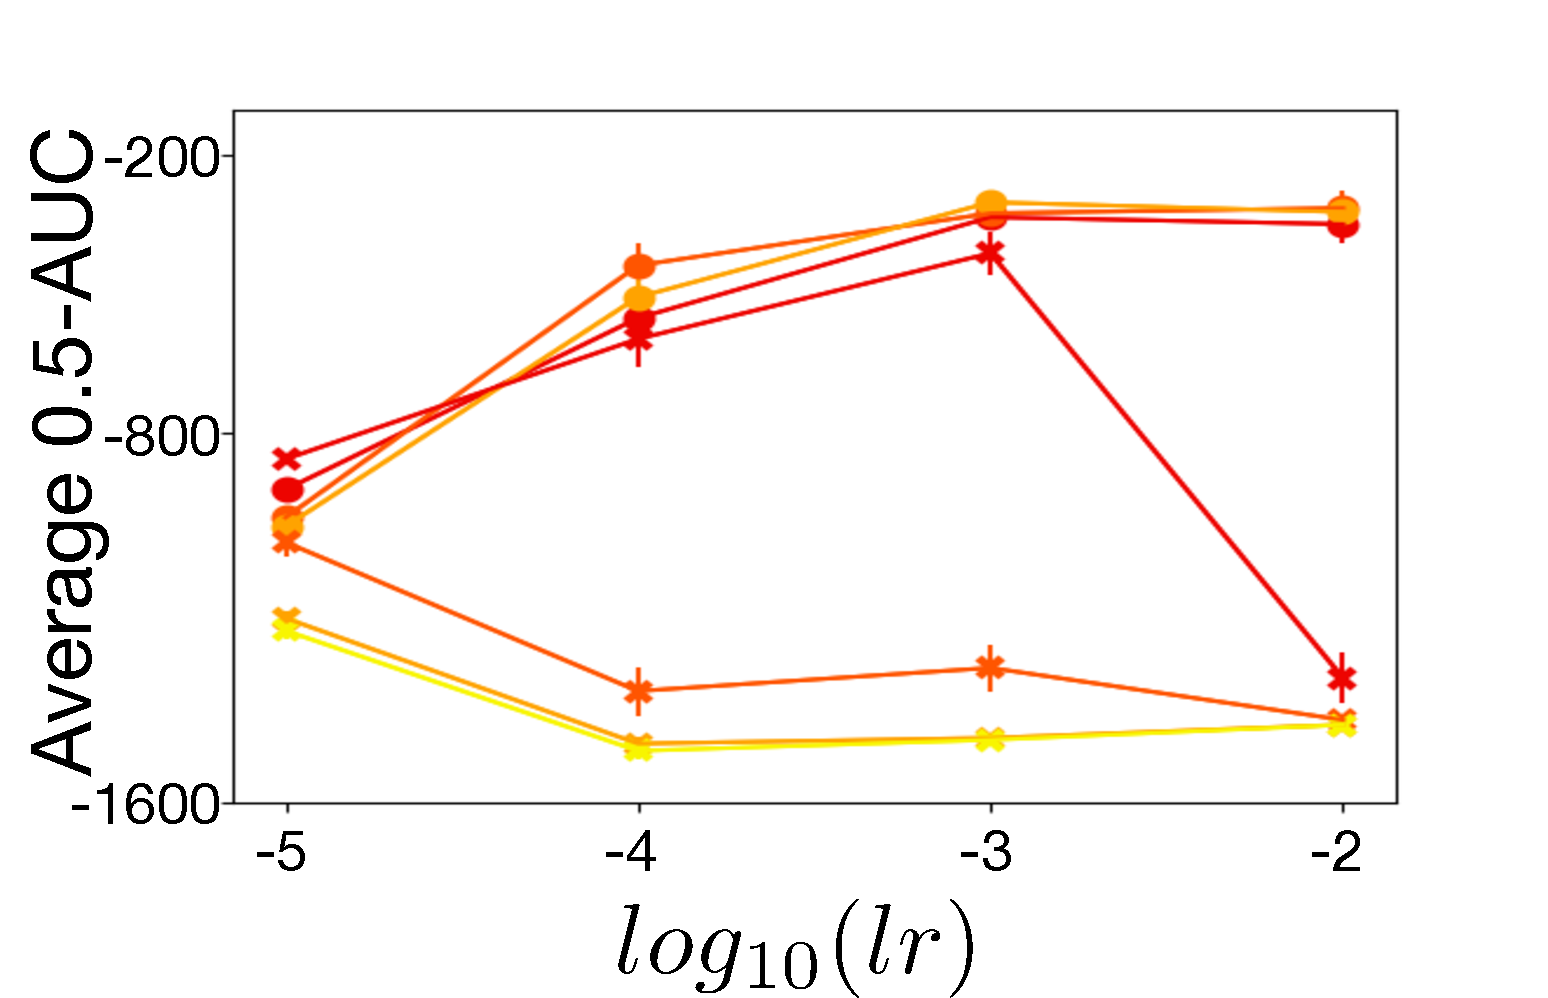
\includegraphics[width=\columnwidth]{figs/deep/continuous/PD_pi_ss.pdf} 
    \caption{Pendulum
    }\label{fig:pendulum-pi}
  \end{subfigure}%
  \begin{subfigure}[b]{0.3\linewidth}
    \centering
    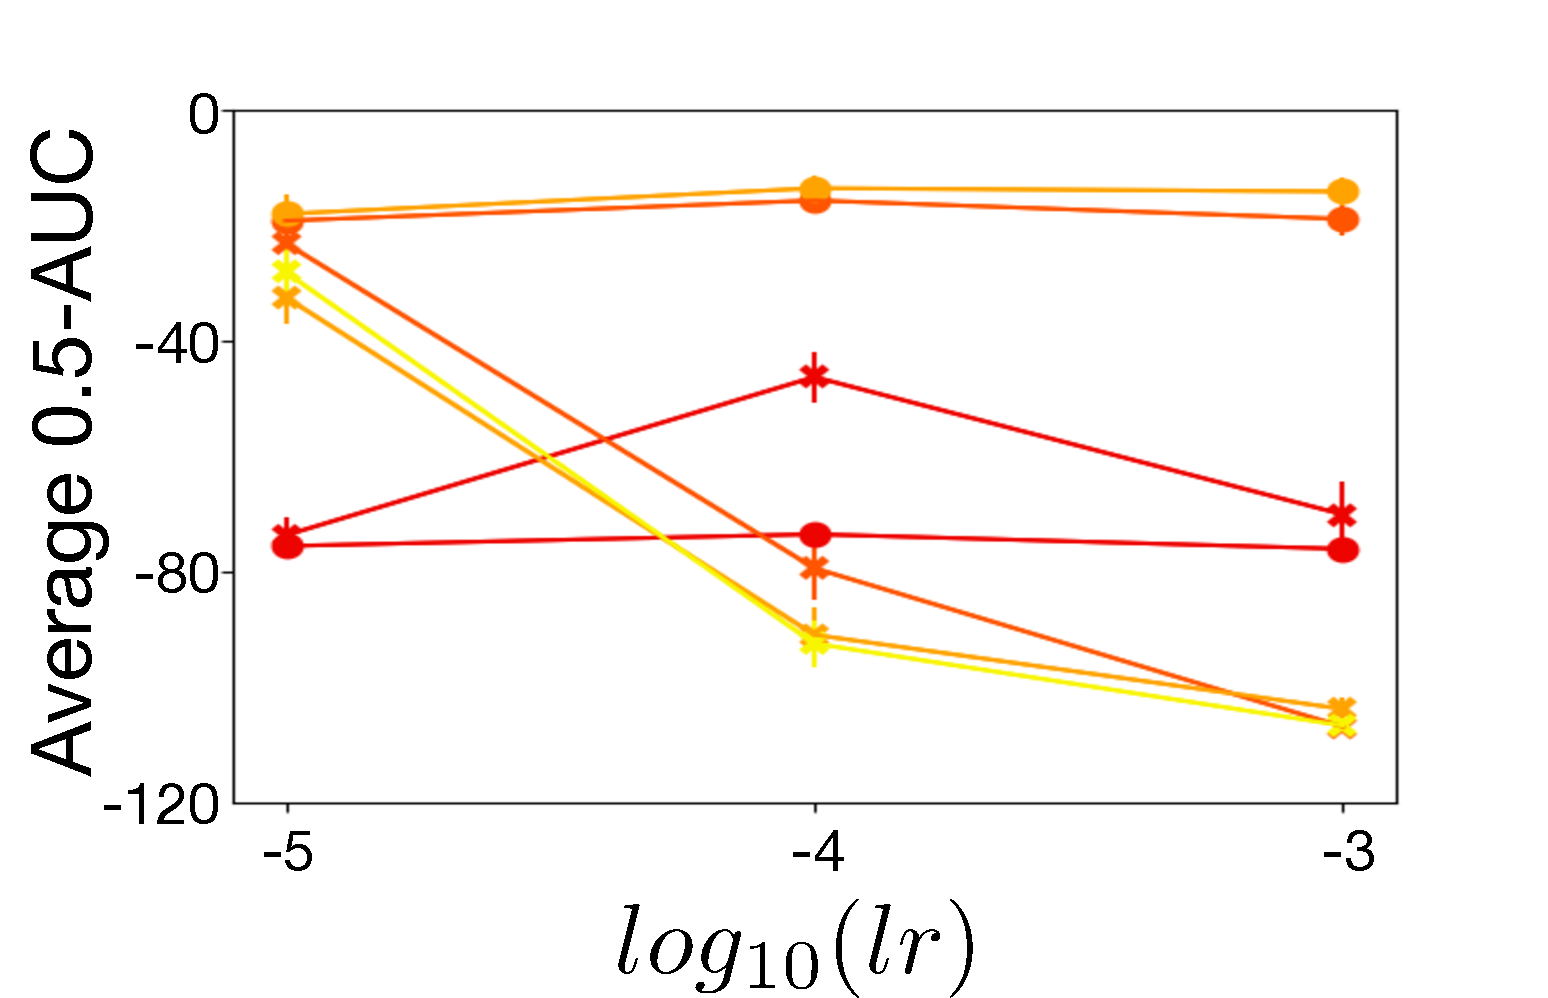
\includegraphics[width=\columnwidth]{figs/deep/continuous/Reacher_pi_ss.pdf} 
    \caption{Reacher
    }\label{fig:reacher-pi}
  \end{subfigure}%
  \begin{subfigure}[b]{0.3\linewidth}
    \centering
    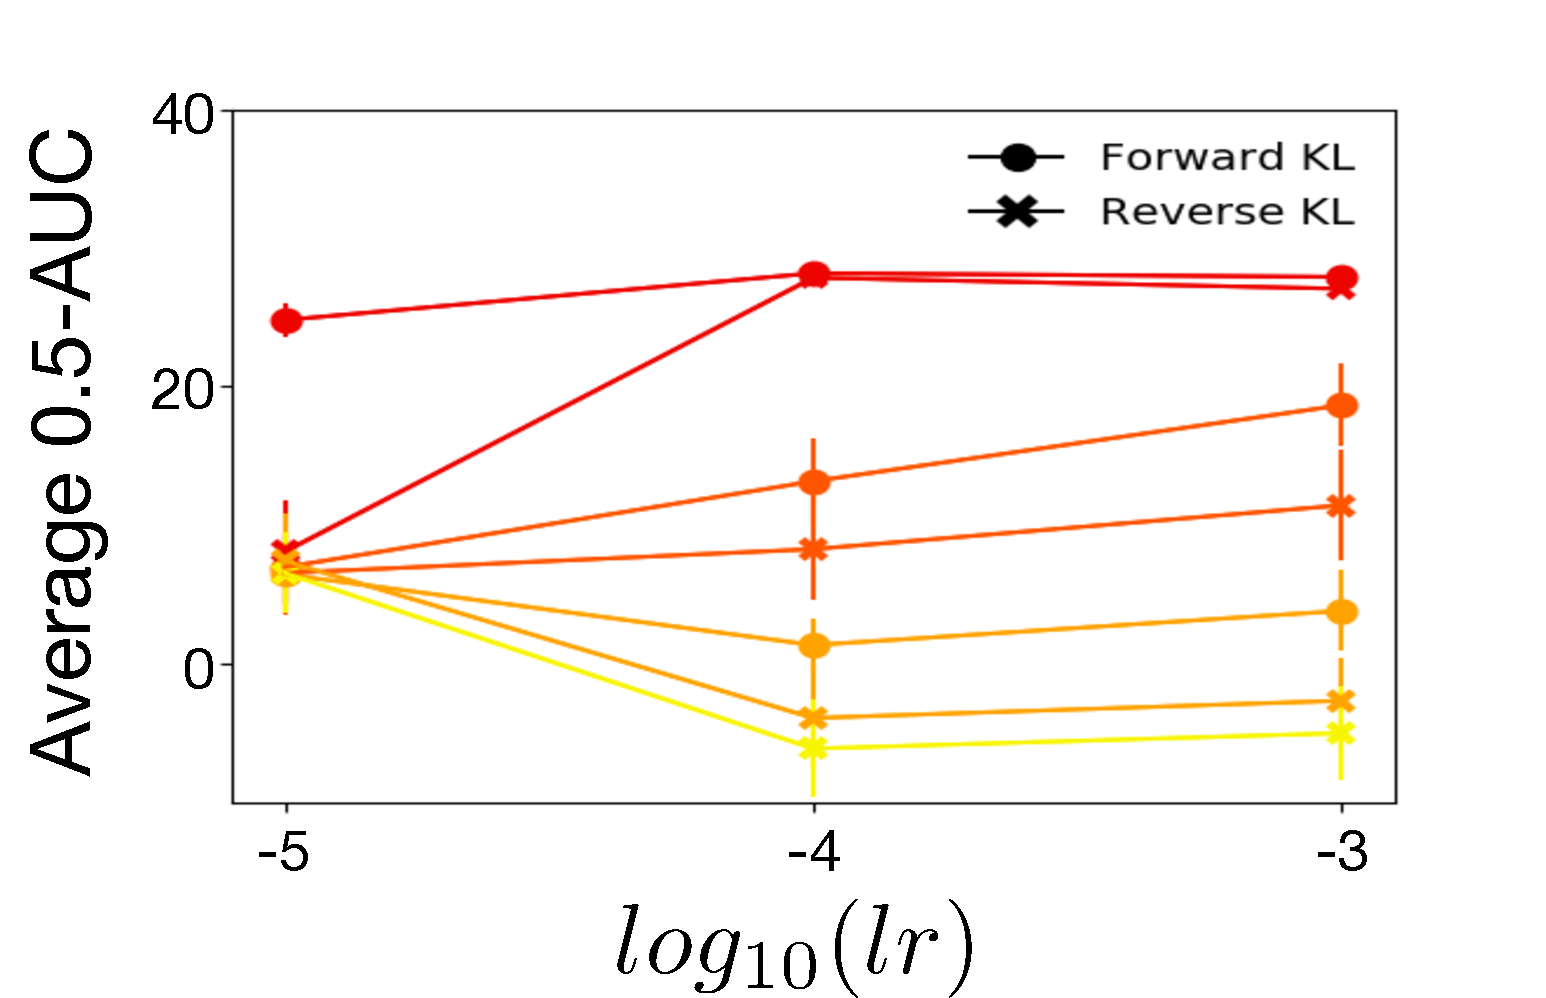
\includegraphics[width=\columnwidth]{figs/deep/continuous/Swimmer_pi_ss.pdf} 
    \caption{Swimmer}
    \label{fig:swimmer-pi}
  \end{subfigure}%
  \caption{Sensitivity plots on different policy learning rates and temperatures for continuous-action environments.}
\end{figure}

\begin{figure}[!ht]
  \centering
  \begin{subfigure}[b]{0.3\linewidth}
    \centering
    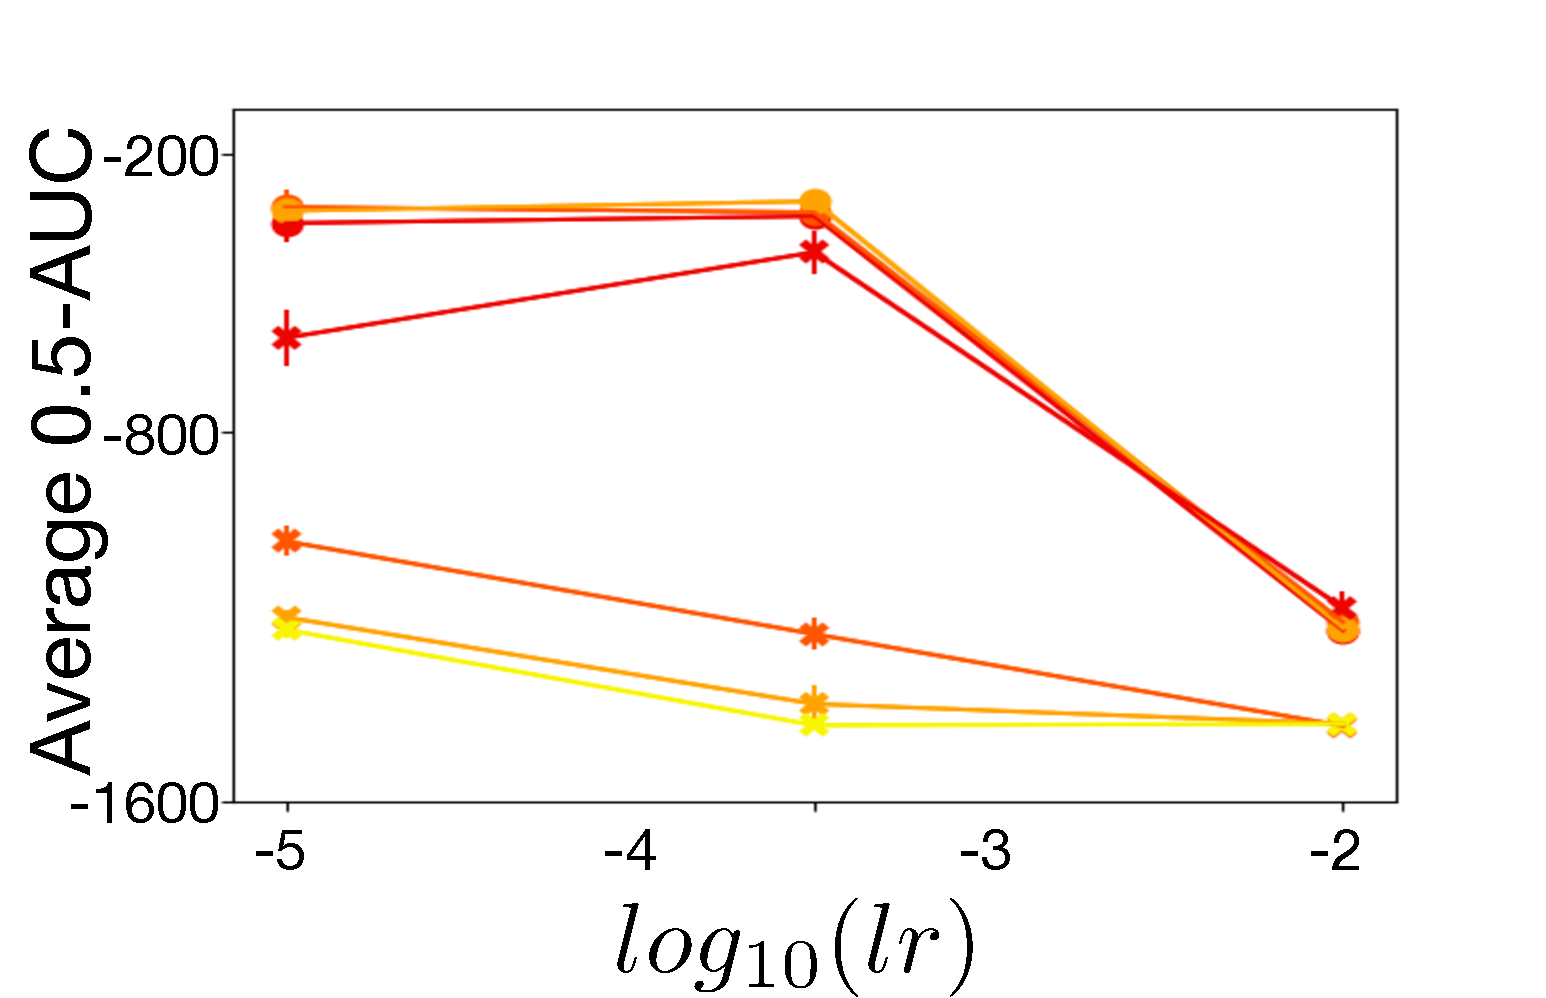
\includegraphics[width=\columnwidth]{figs/deep/continuous/PD_qv_ss.pdf} 
    \caption{Pendulum
    }\label{fig:pendulum-pi}
  \end{subfigure}%
  \begin{subfigure}[b]{0.3\linewidth}
    \centering
    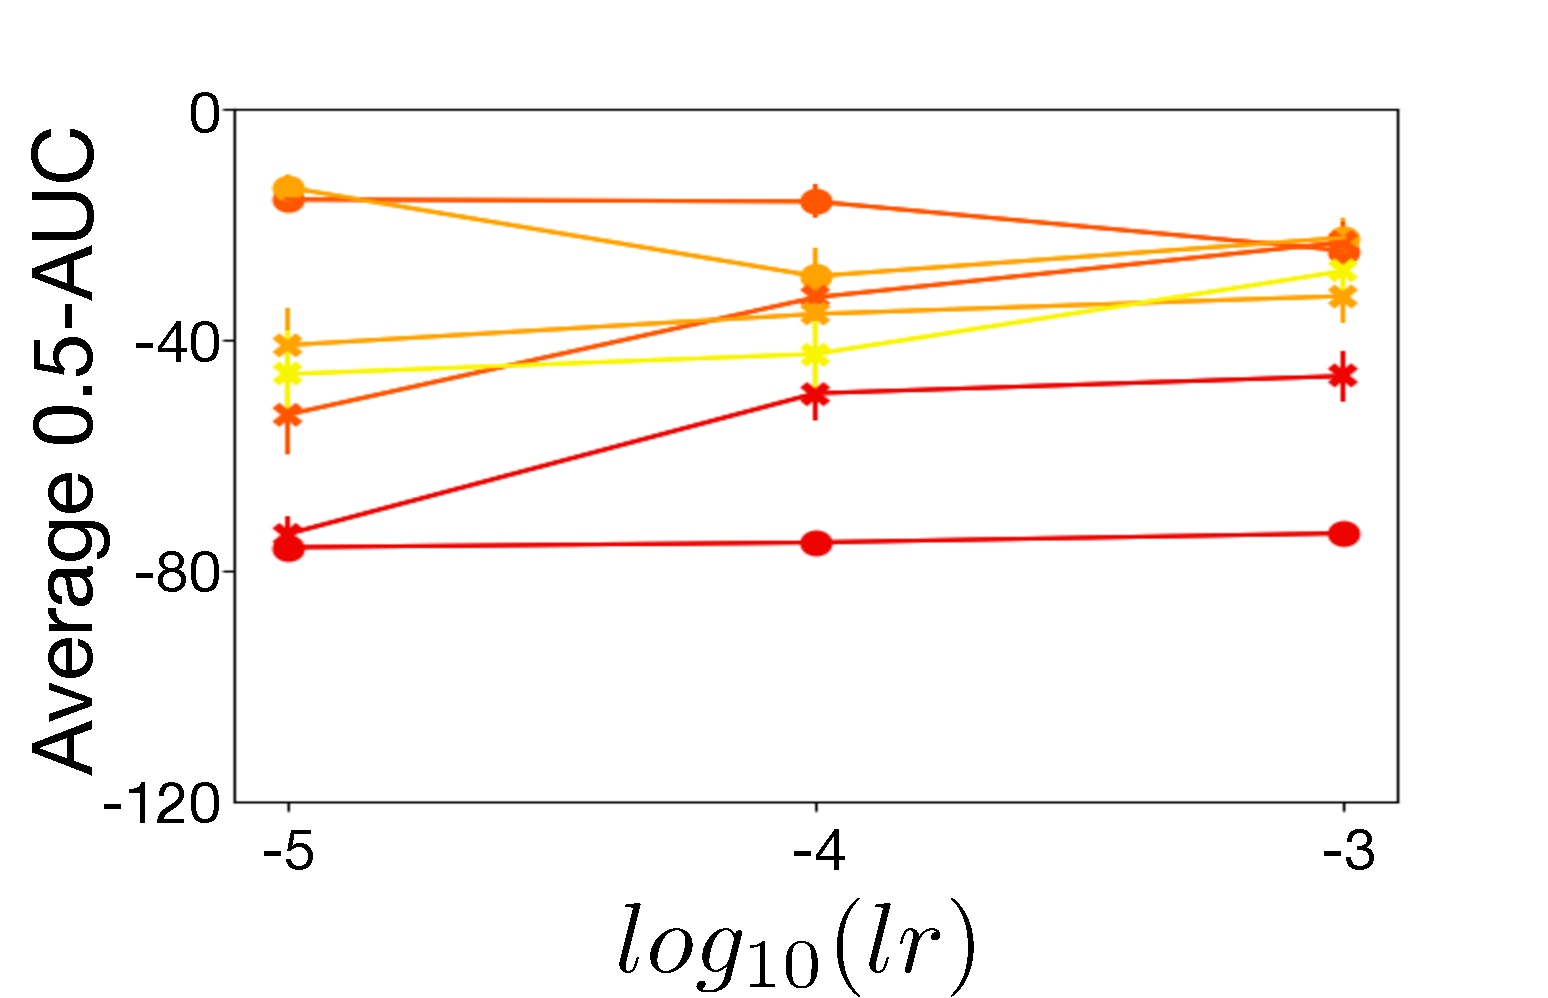
\includegraphics[width=\columnwidth]{figs/deep/continuous/Reacher_qv_ss.pdf} 
    \caption{Reacher
    }\label{fig:reacher-pi}
  \end{subfigure}%
  \begin{subfigure}[b]{0.3\linewidth}
    \centering
    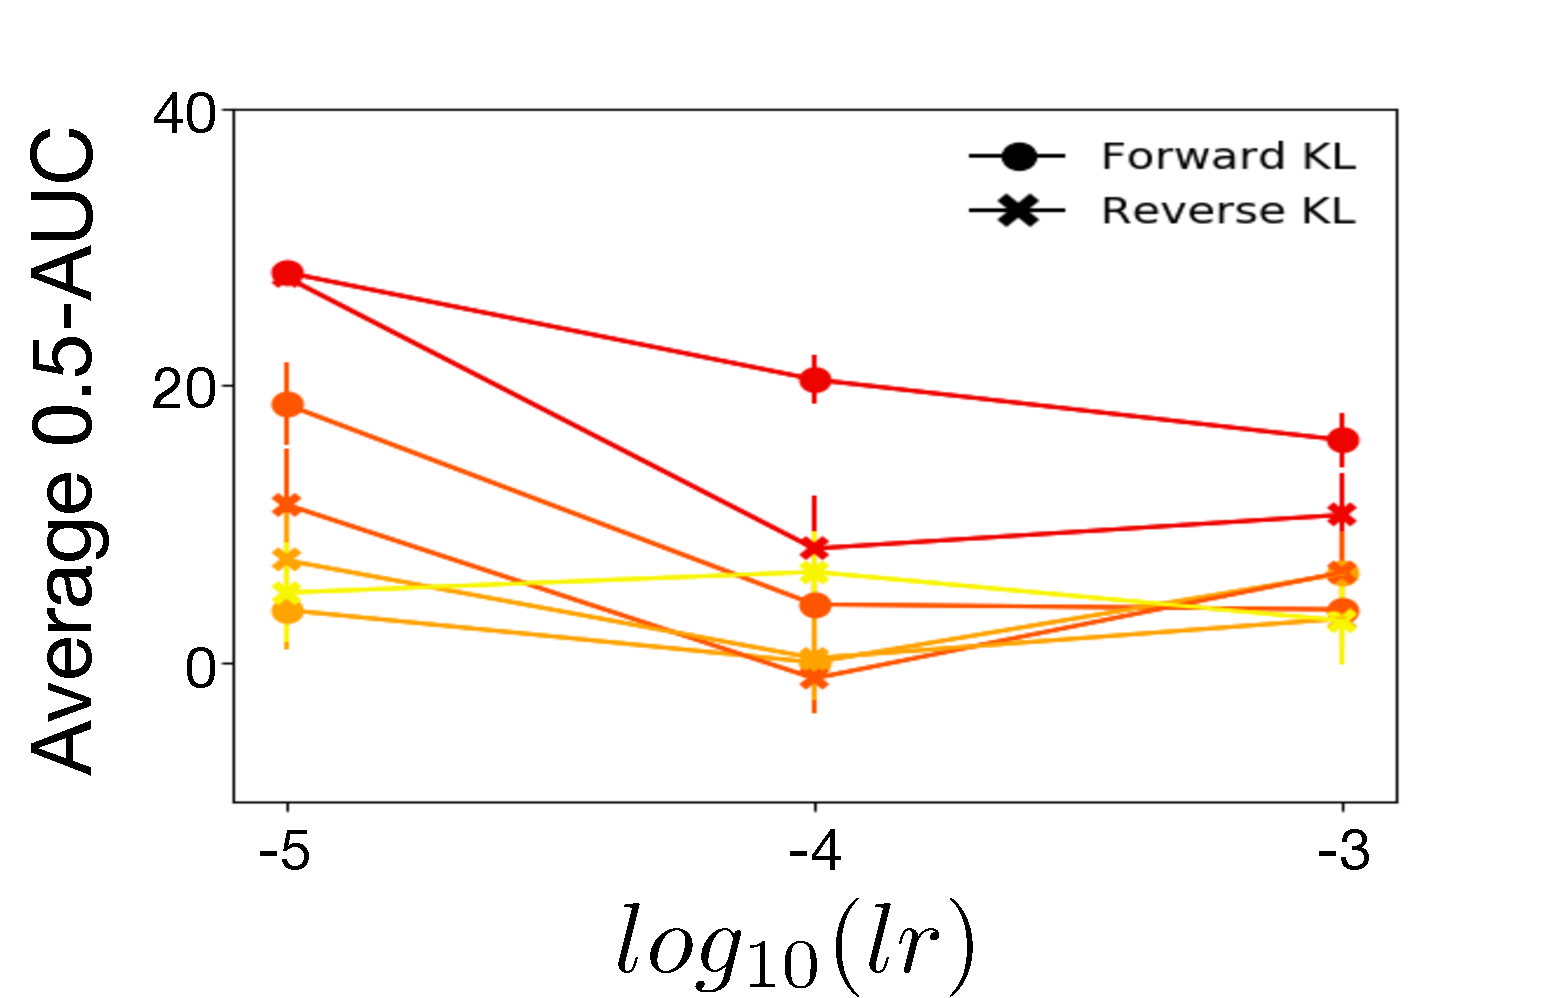
\includegraphics[width=\columnwidth]{figs/deep/continuous/Swimmer_qv_ss.pdf} 
    \caption{Swimmer}
    \label{fig:swimmer-pi}
  \end{subfigure}%
  \caption{Sensitivity plots on different value-function learning rates and temperatures for continuous-action environments.}
\end{figure}

\subsection{Discrete Actions}
We show sensitivity plots relative to the learning rates $\{10^{-5}, 10^{-4}, 10^{-3}\}$ for all temperatures $\{0, 0.01, 0.1, 1\}$ and both FKL and RKL.
\begin{figure}[!ht]
  \centering
  \begin{subfigure}[b]{0.25\linewidth}
    \centering
    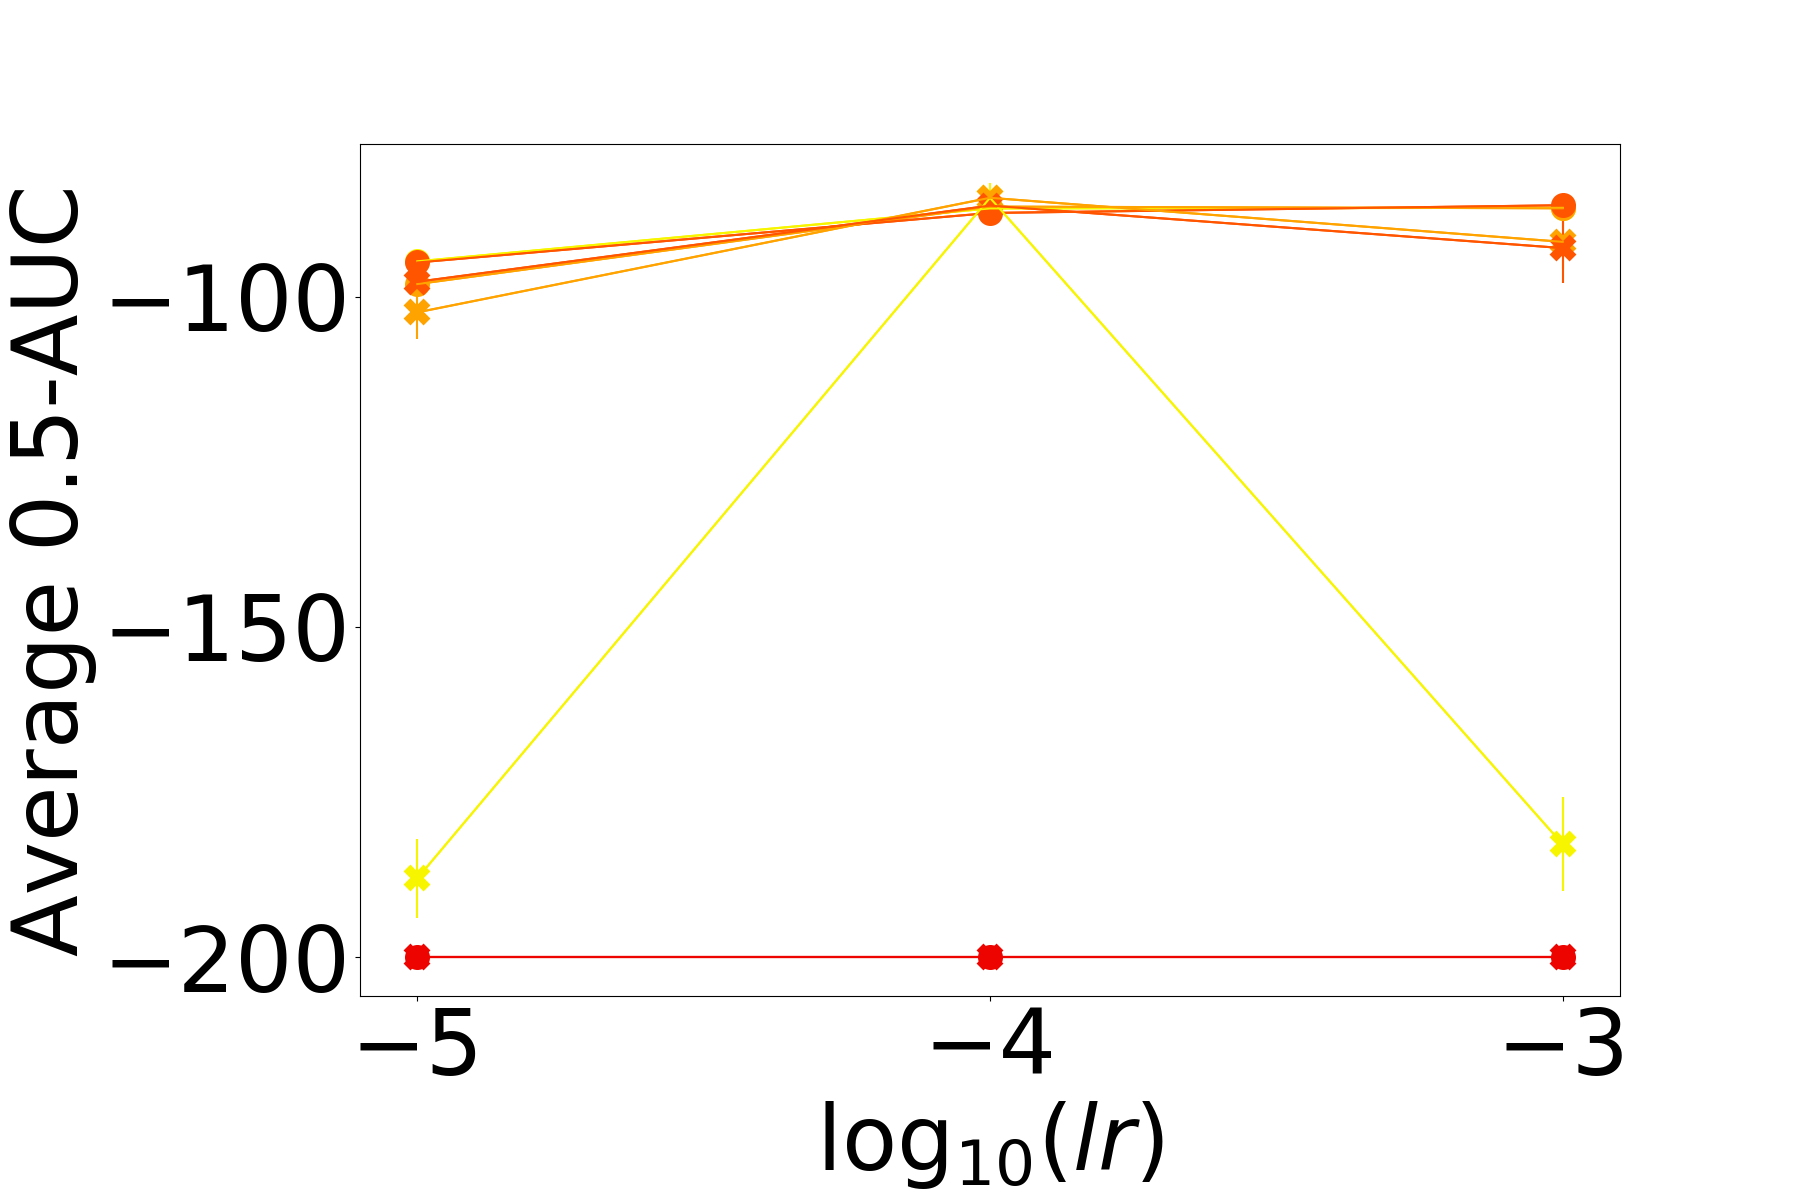
\includegraphics[width=\columnwidth]{figs/deep/discrete/sensitivity/UNLABELED_kl_auc-0.5_Acrobot_lr_sensitivity.png} 
    \caption{Acrobot
    }\label{fig:acrobot}
  \end{subfigure}%
  \begin{subfigure}[b]{0.25\linewidth}
    \centering
    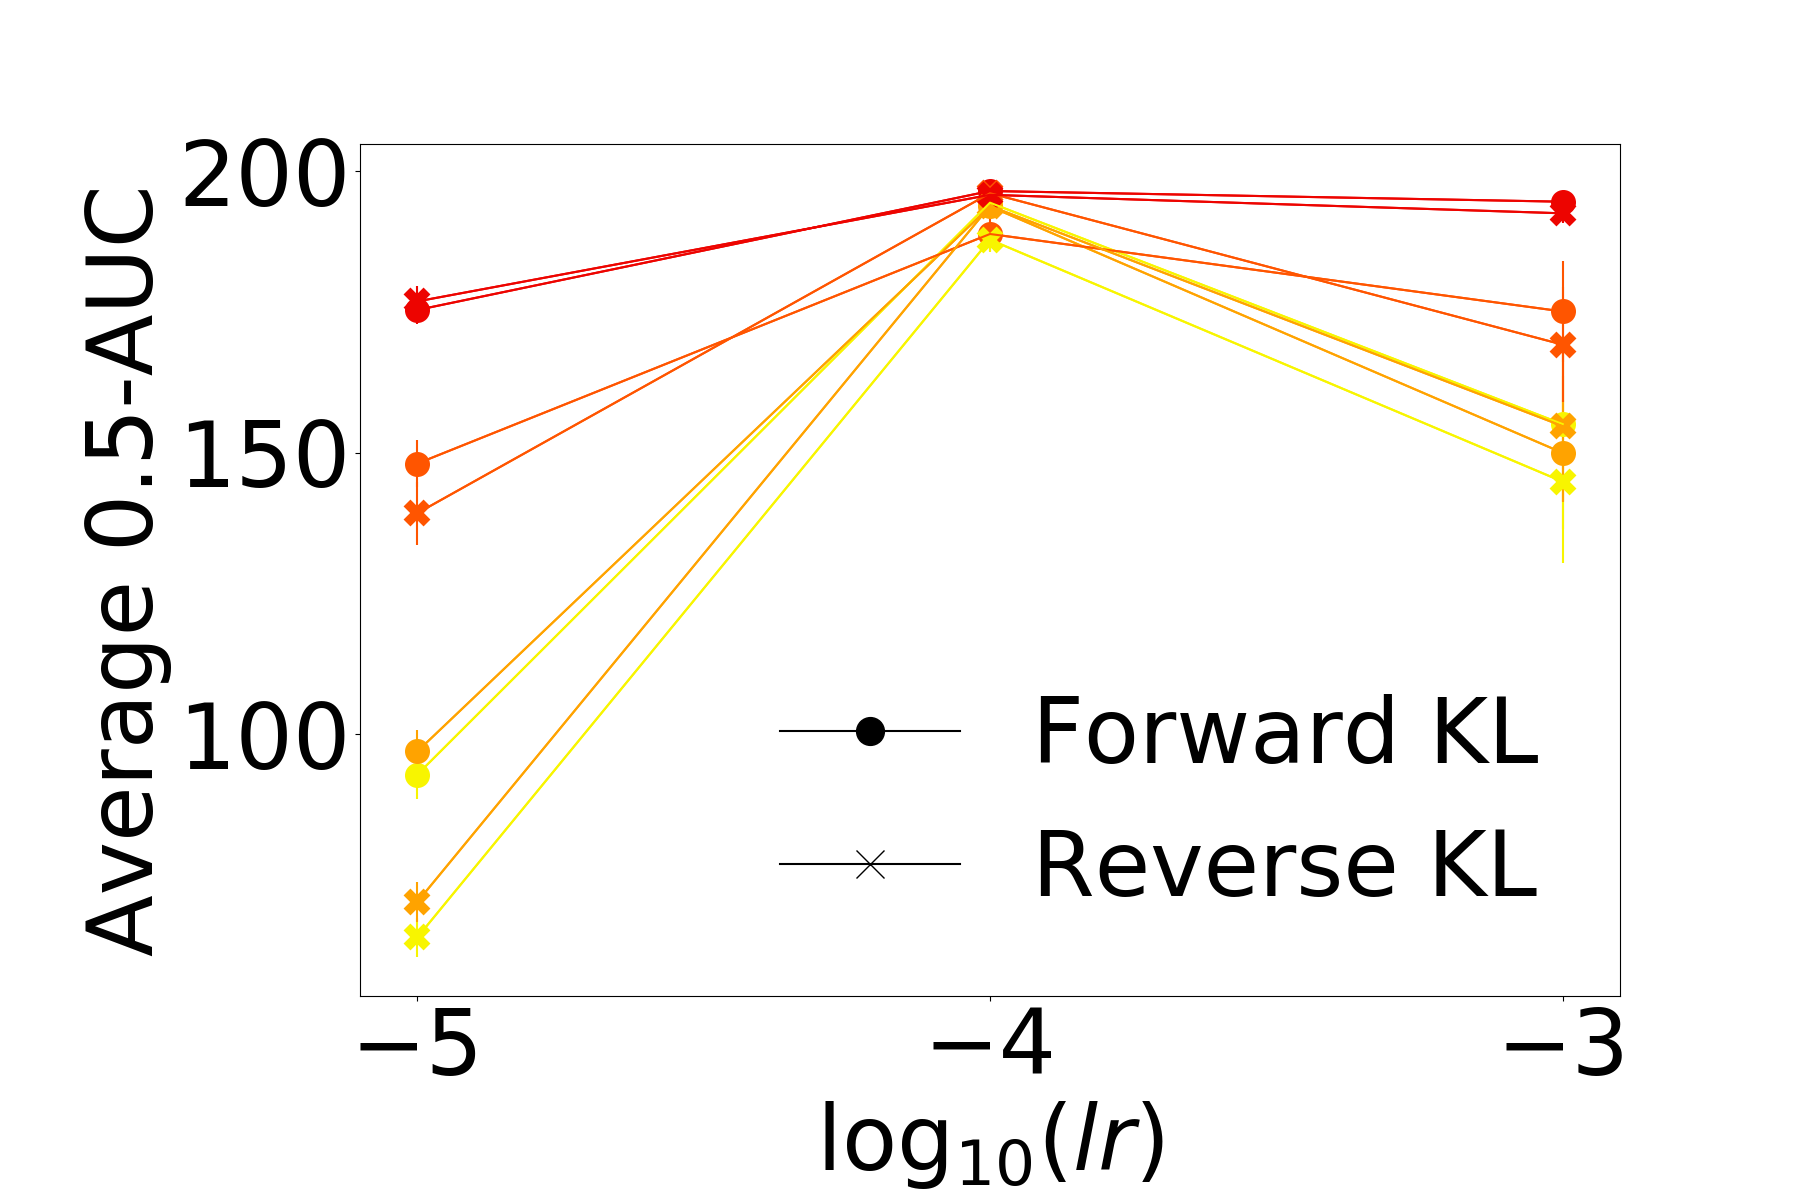
\includegraphics[width=\columnwidth]{figs/deep/discrete/sensitivity/kl_auc-0.5_CartPole_lr_sensitivity.png} 
    \caption{Cartpole
    }\label{fig:cartpole}
  \end{subfigure}%
  \begin{subfigure}[b]{0.25\linewidth}
    \centering
    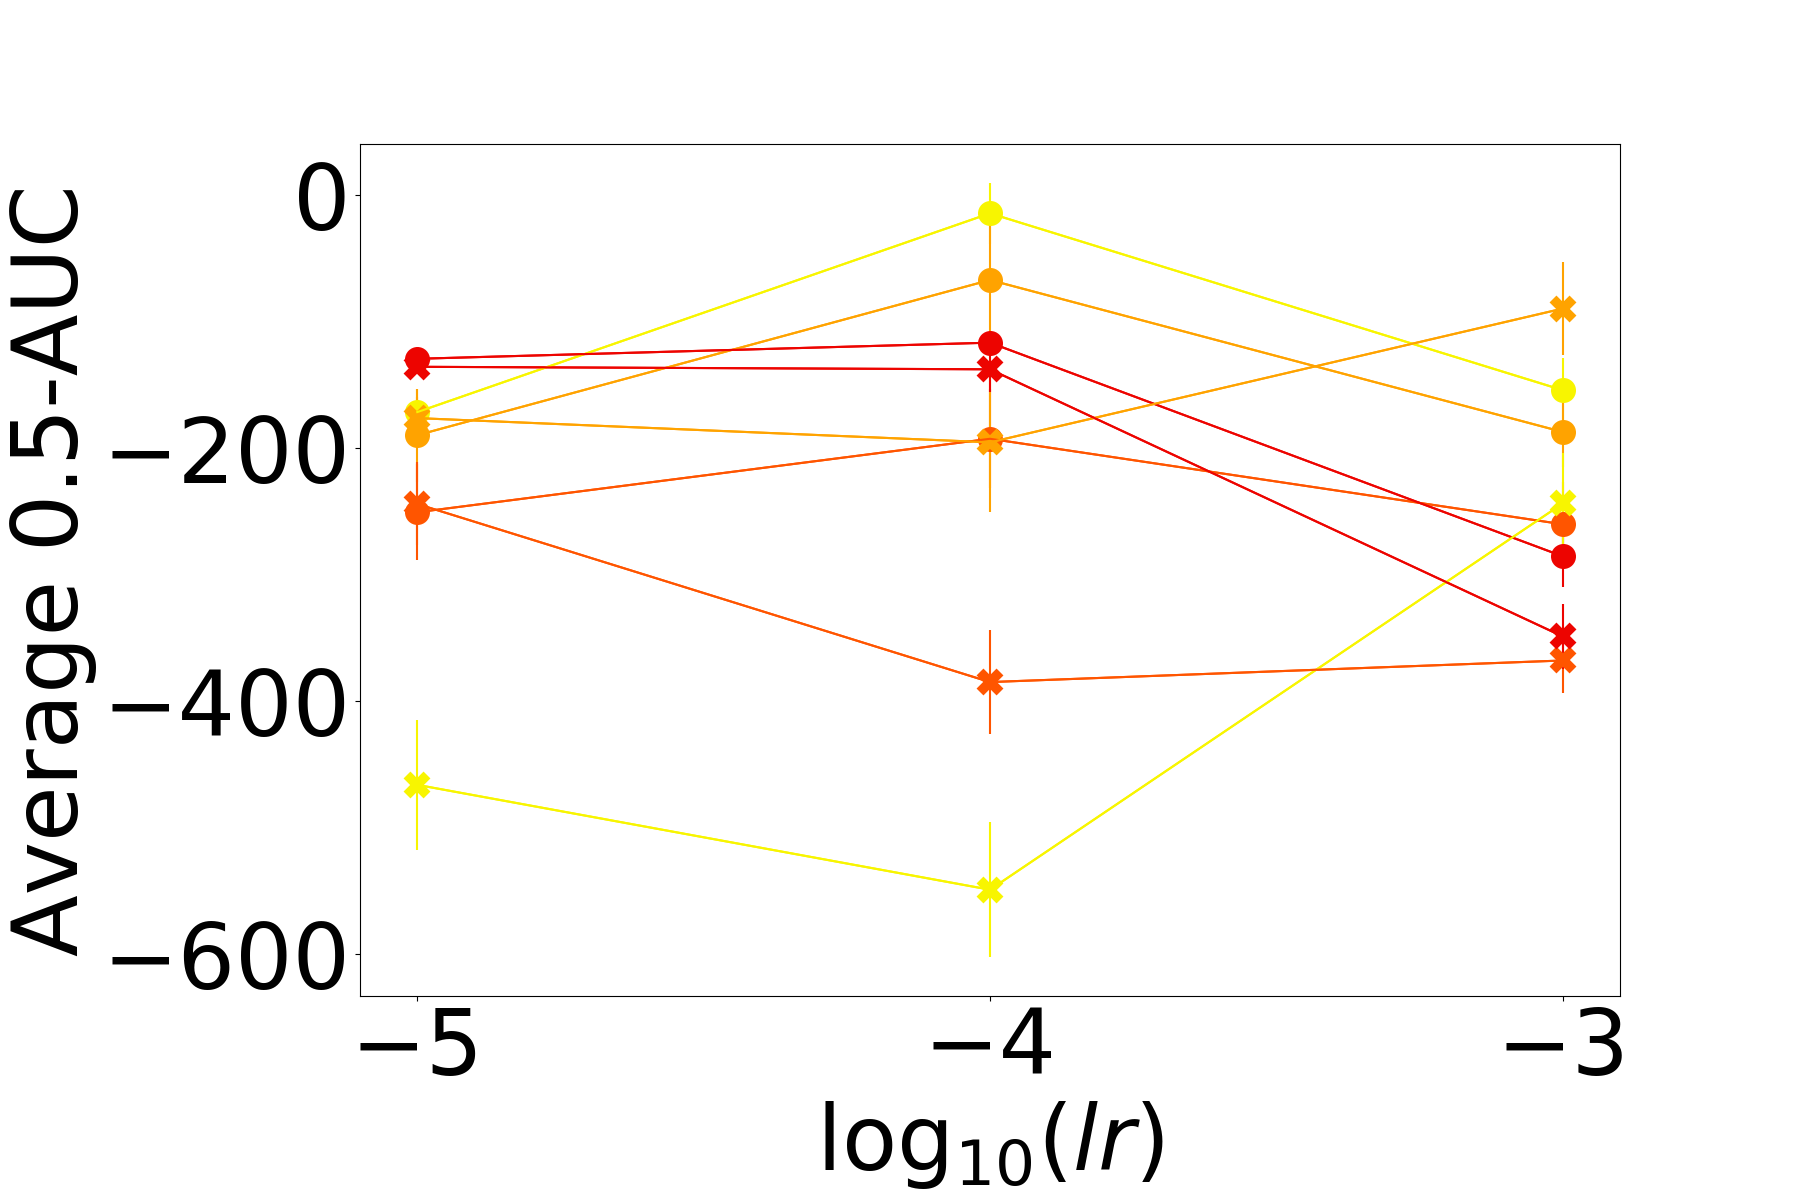
\includegraphics[width=\columnwidth]{figs/deep/discrete/sensitivity/UNLABELED_kl_auc-0.5_LunarLander_lr_sensitivity.png} 
    \caption{Lunar Lander}
    \label{fig:lunar-lander}
  \end{subfigure}%
  \begin{subfigure}[b]{0.25\linewidth}
    \centering
    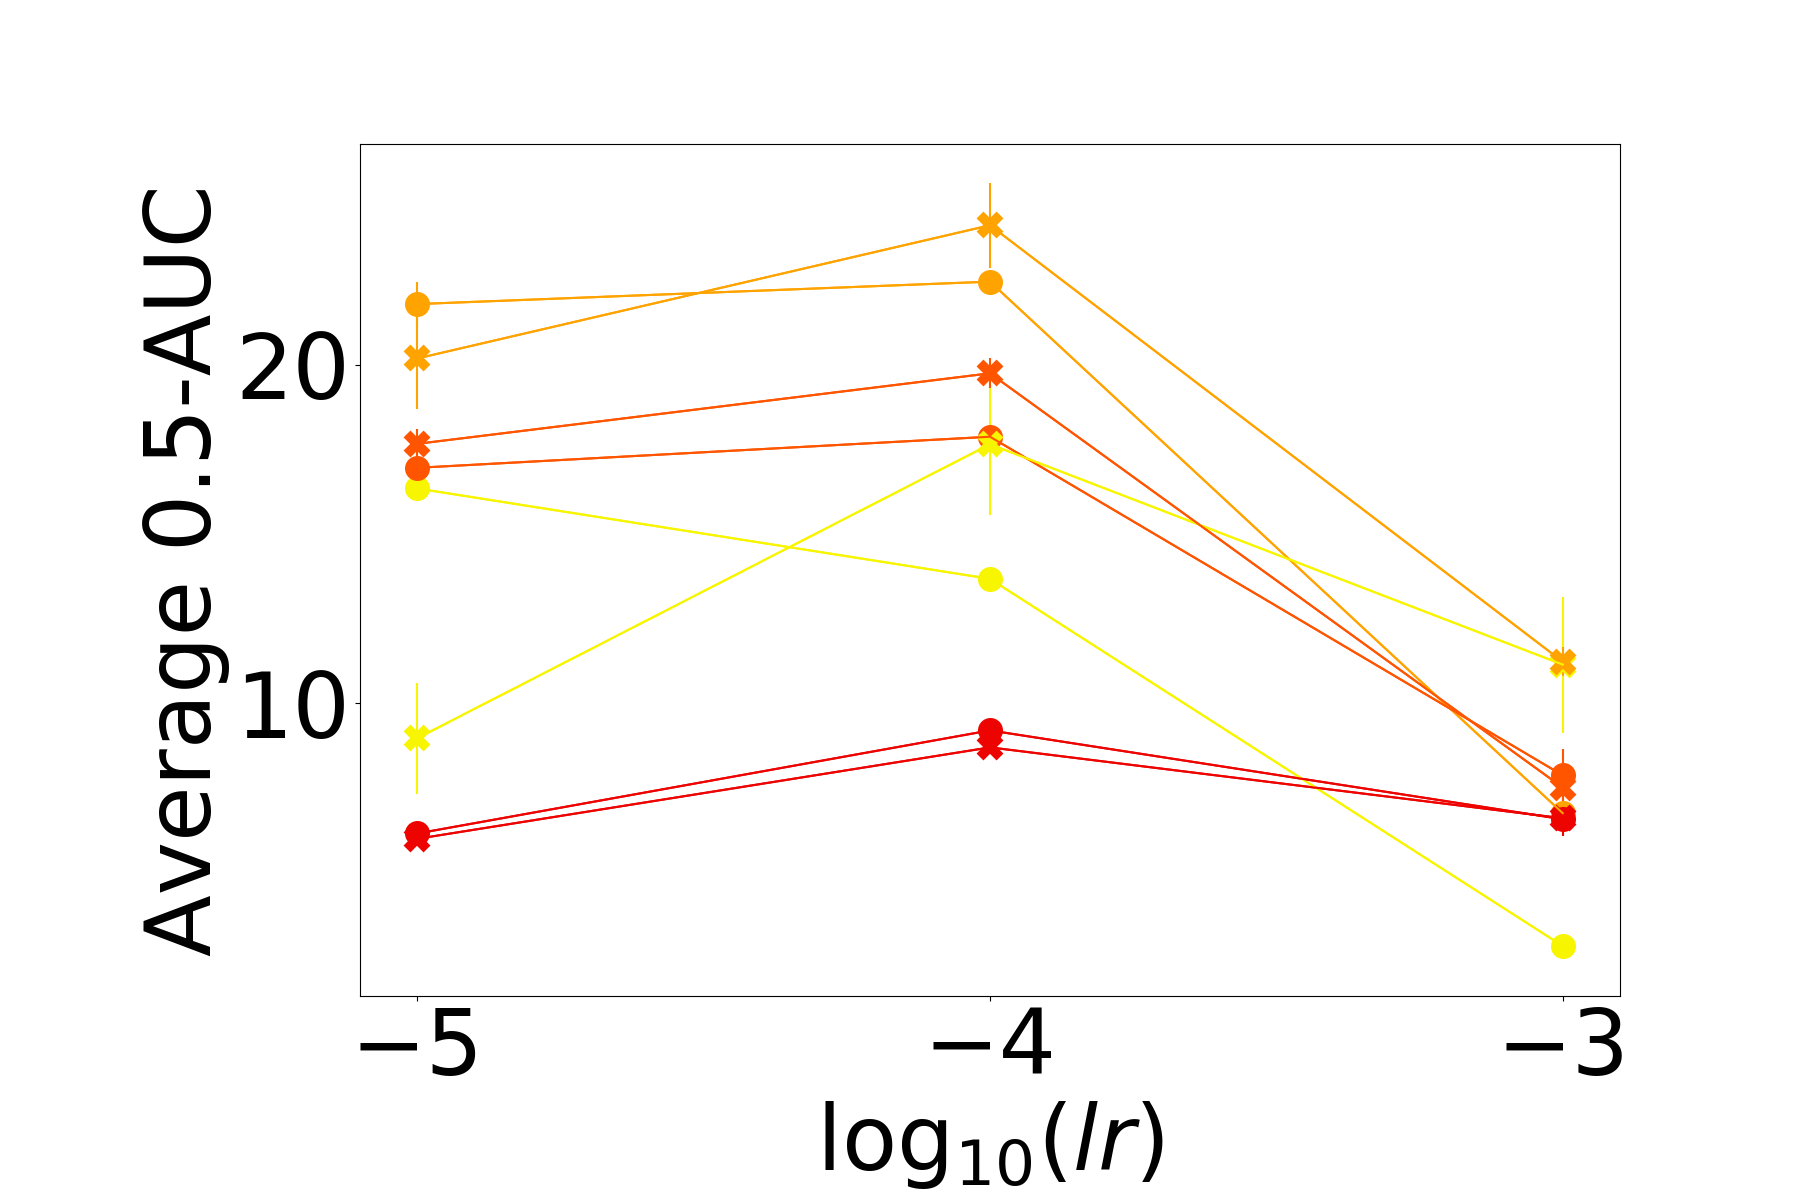
\includegraphics[width=\columnwidth]{figs/deep/discrete/sensitivity/UNLABELED_kl_auc-0.5_asterix_lr_sensitivity.png} 
    \caption{Asterix
    }\label{fig:asterix}
  \end{subfigure}%
  
  \begin{subfigure}[b]{0.25\linewidth}
    \centering
    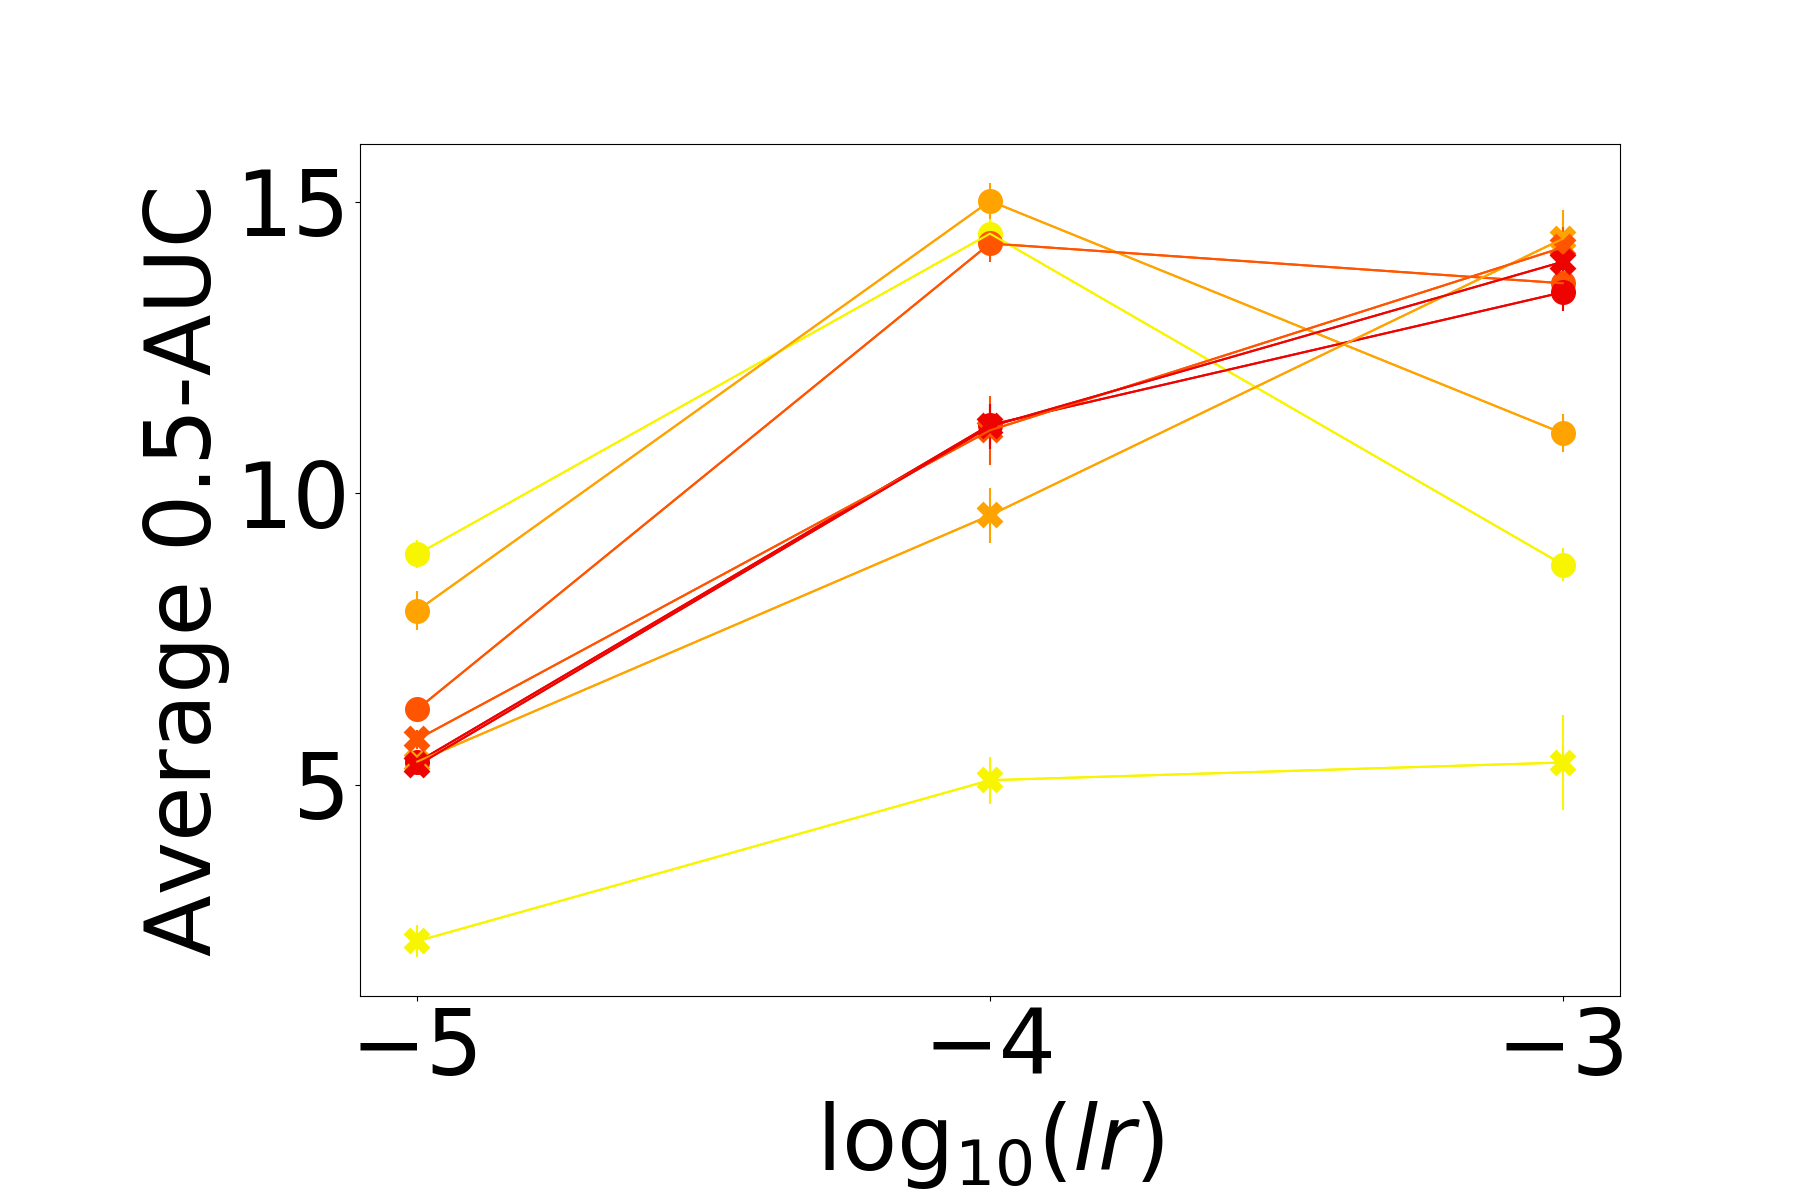
\includegraphics[width=\columnwidth]{figs/deep/discrete/sensitivity/UNLABELED_kl_auc-0.5_breakout_lr_sensitivity.png} 
    \caption{Breakout
    }\label{fig:breakout}
  \end{subfigure}%
  \begin{subfigure}[b]{0.25\linewidth}
    \centering
    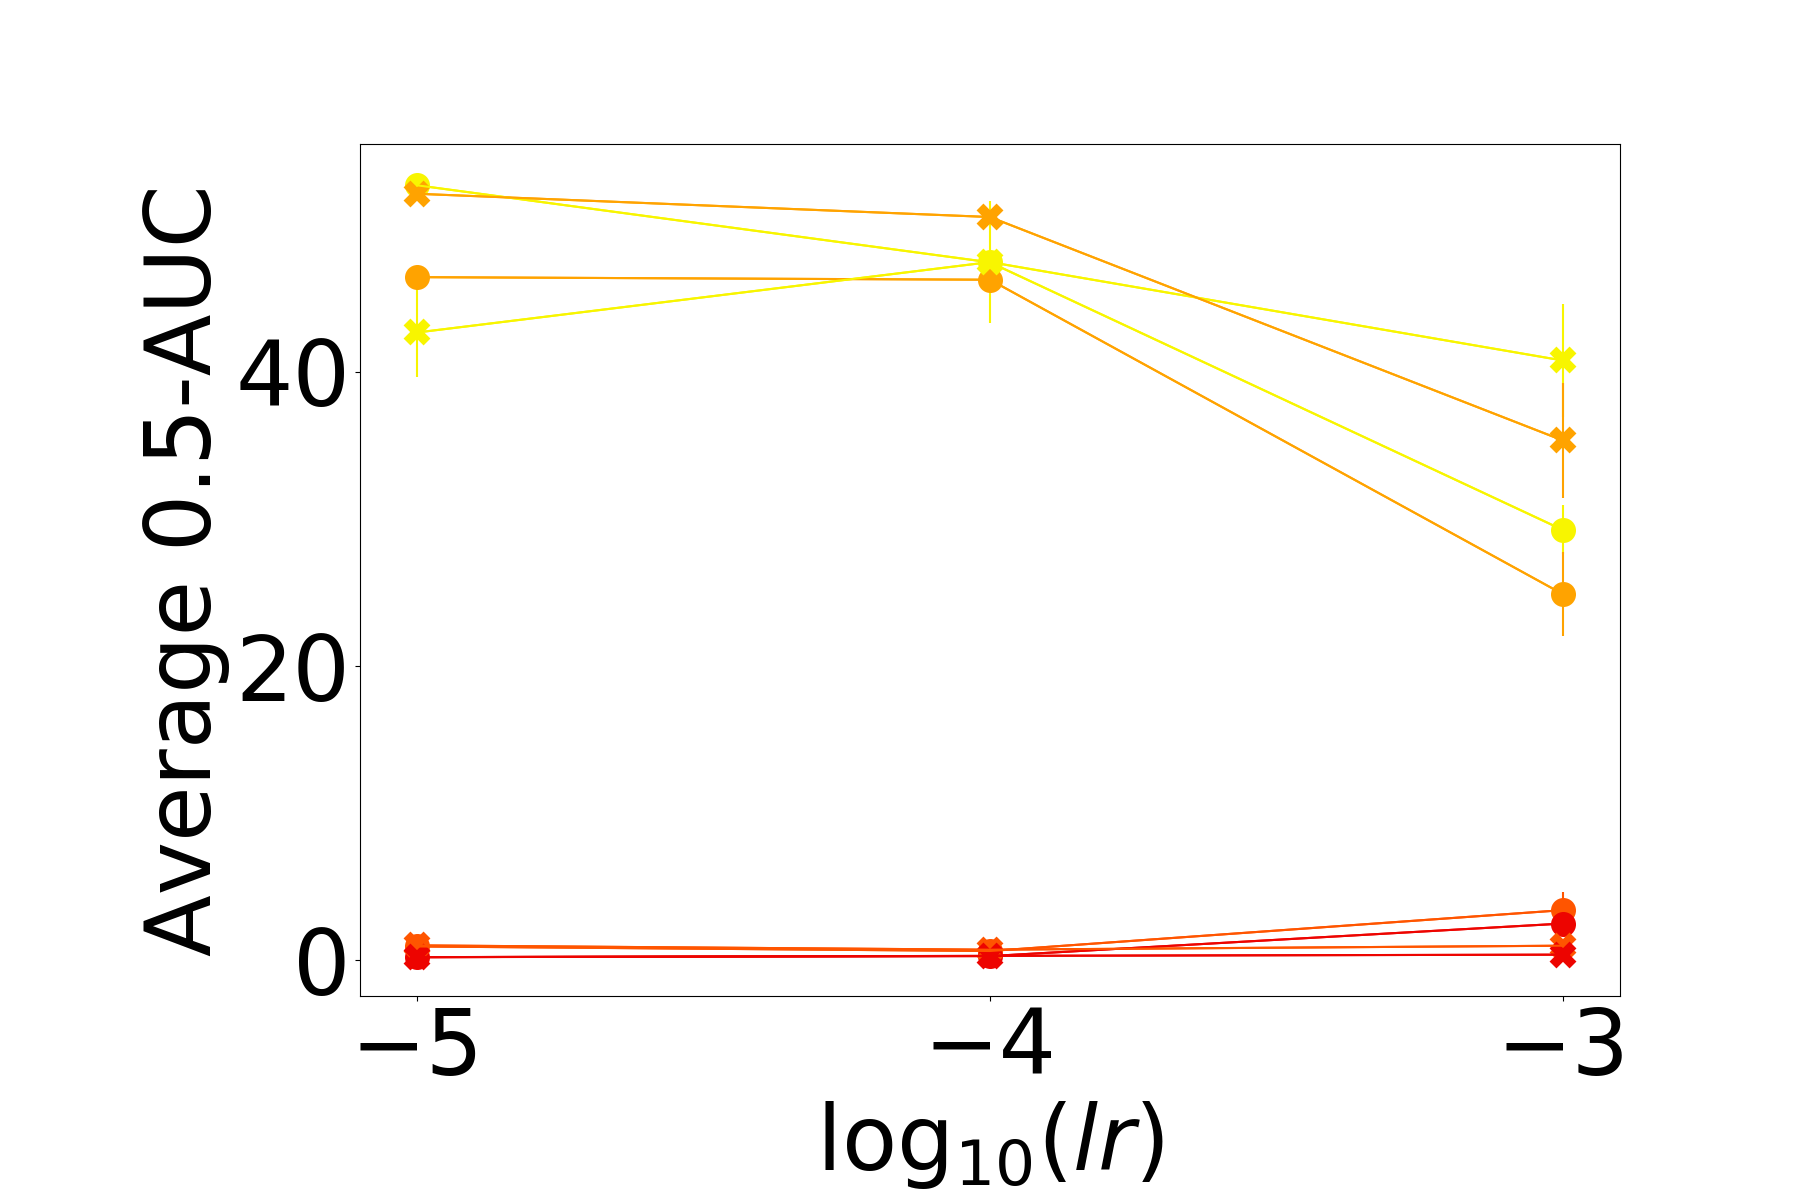
\includegraphics[width=\columnwidth]{figs/deep/discrete/sensitivity/UNLABELED_kl_auc-0.5_freeway_lr_sensitivity.png} 
    \caption{Freeway
    }\label{fig:freeway}
  \end{subfigure}%
  \begin{subfigure}[b]{0.25\linewidth}
    \centering
    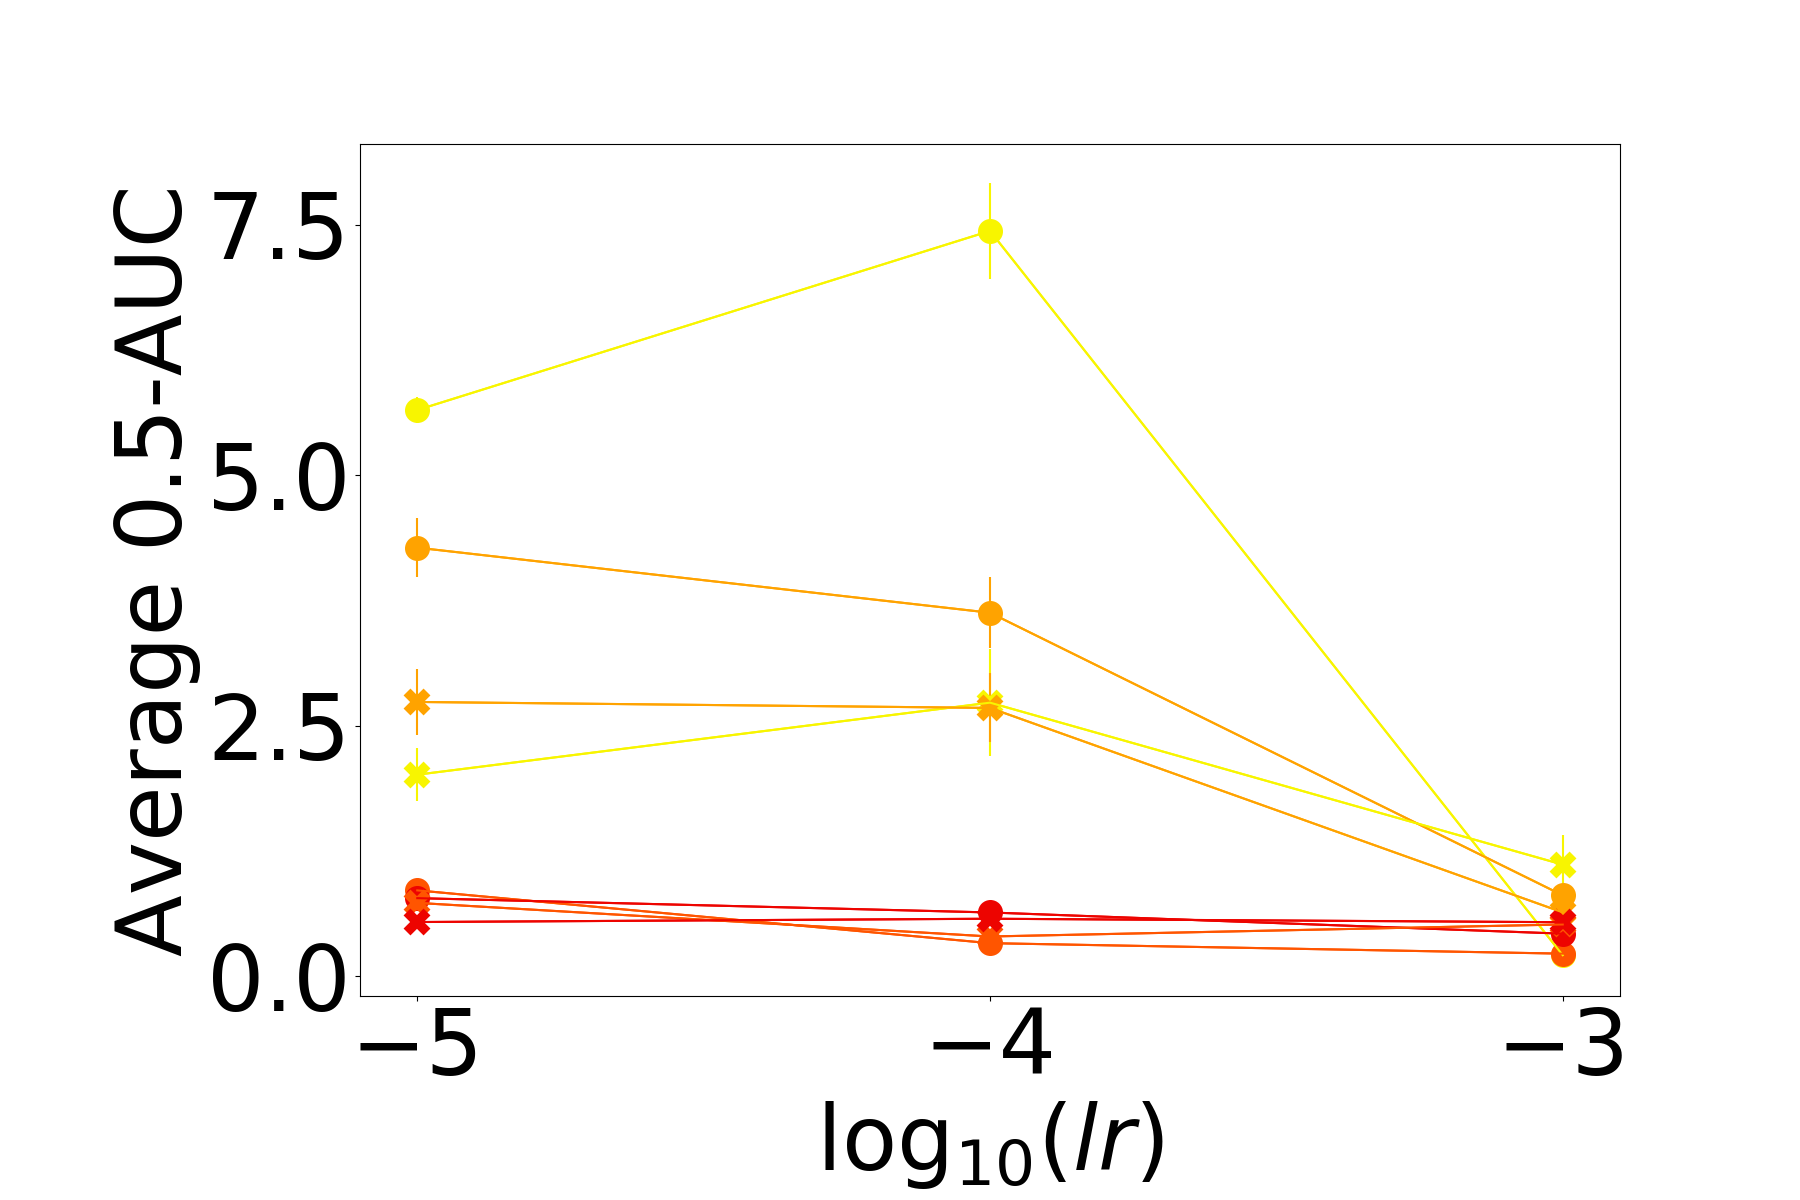
\includegraphics[width=\columnwidth]{figs/deep/discrete/sensitivity/UNLABELED_kl_auc-0.5_seaquest_lr_sensitivity.png} 
    \caption{Seaquest
    }\label{fig:seaquest}
  \end{subfigure}%
  \begin{subfigure}[b]{0.25\linewidth}
    \centering
    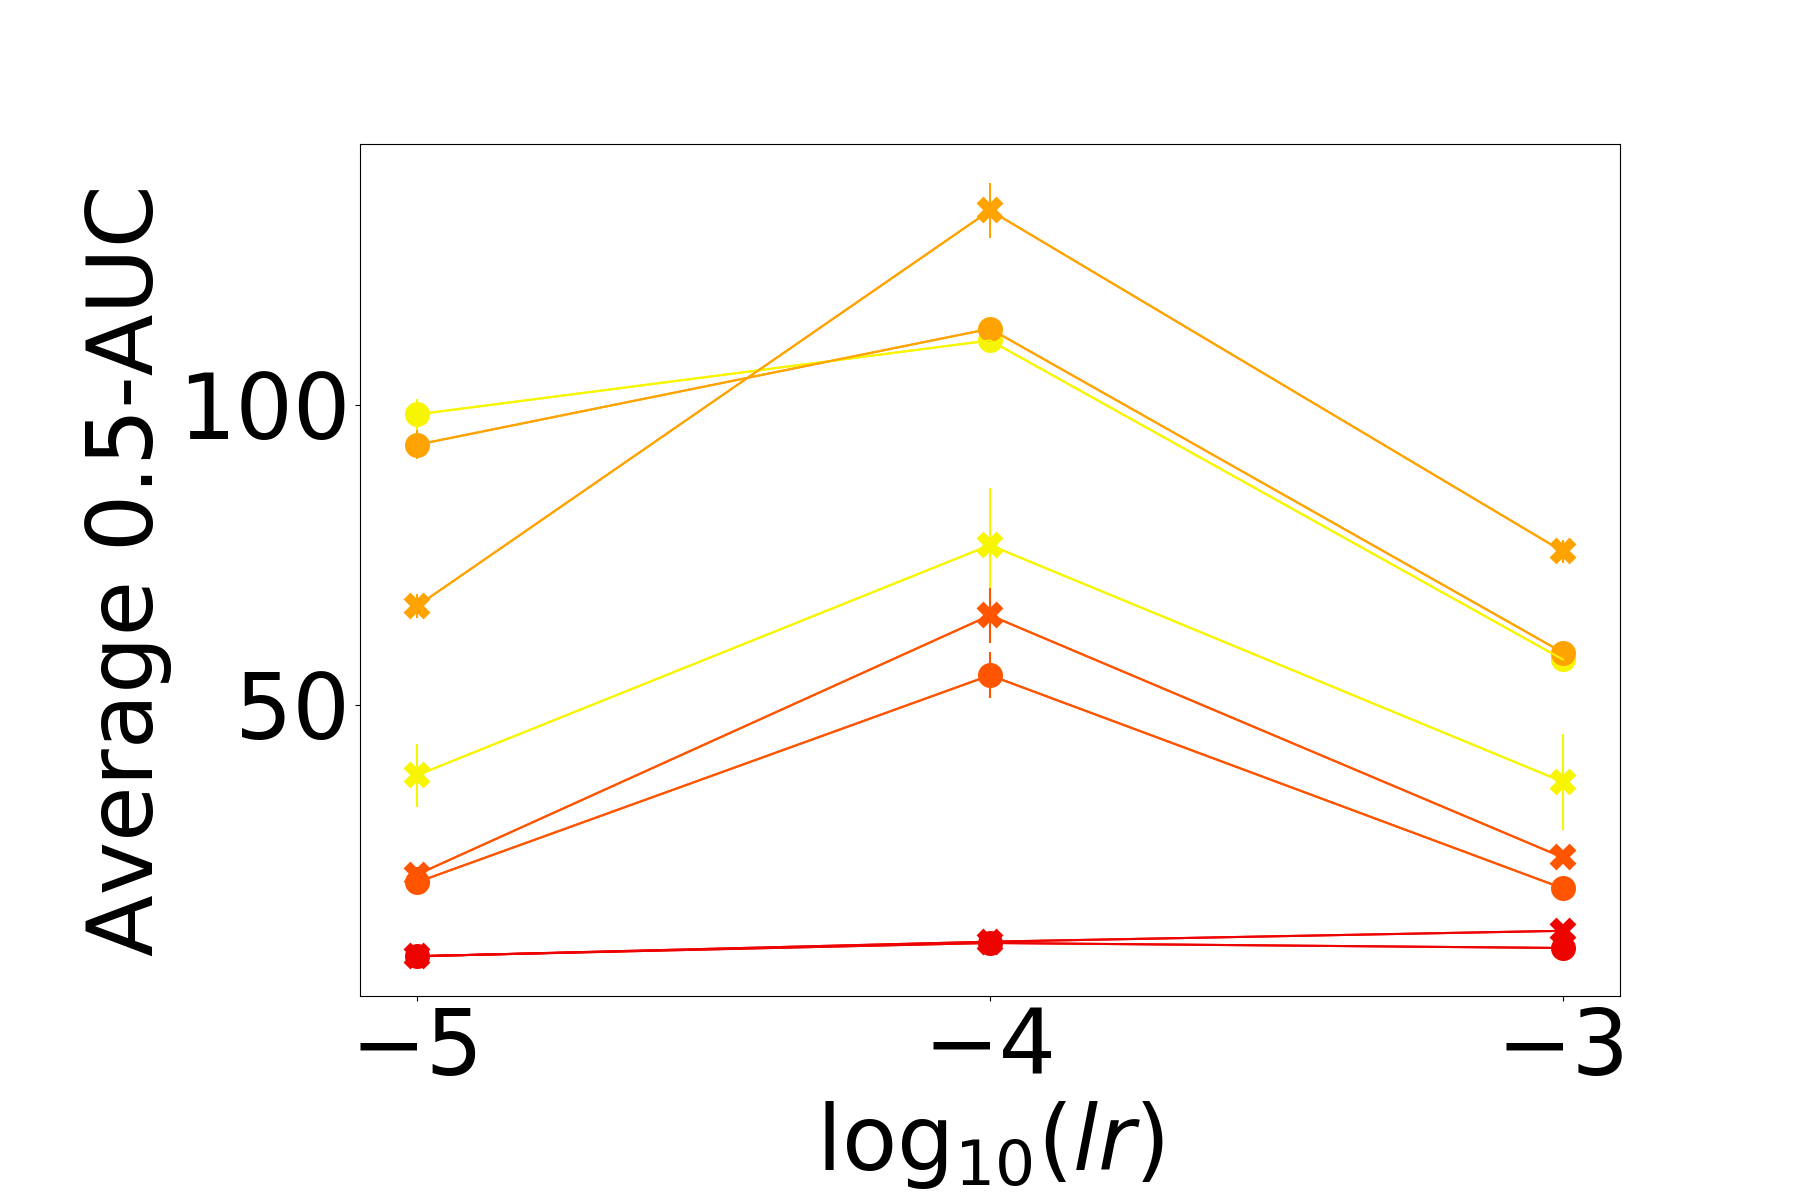
\includegraphics[width=\columnwidth]{figs/deep/discrete/sensitivity/UNLABELED_kl_auc-0.5_space_invaders_lr_sensitivity.png} 
    \caption{Space Invaders
    }\label{fig:space-invaders}
  \end{subfigure}
  \caption{Sensitivity plots on different learning rates and temperatures for discrete-action environments.}
\end{figure}


\clearpage

\section{Additional Plots}\label{sec:more-plots}

\subsection{Continuous Bandits - Optimization Surface}\label{sec:bandit-plots}
In this section we include additional heatmap results to help understand our results better.

\Cref{fig:bandit-heatmap-reduced-pts} shows heatmaps using reduced number of numerical integration points (128 points). FKL loss surface shows no difference compared to using more points but RKL loss surface shows wavelet patterns along the top edges.

\Cref{fig:bandit-heatmap-non-tanh} shows the KL loss surface of the Gaussian policy without $\tanh$ transformation. Suboptima appears at bottom edges in RKL. 

% We find this suboptima is due to the truncation of numerical integration points of magnitudes larger than 0.95 for stability, but is less problematic when applying $\tanh$ transformation.

\begin{figure}
    \centering
    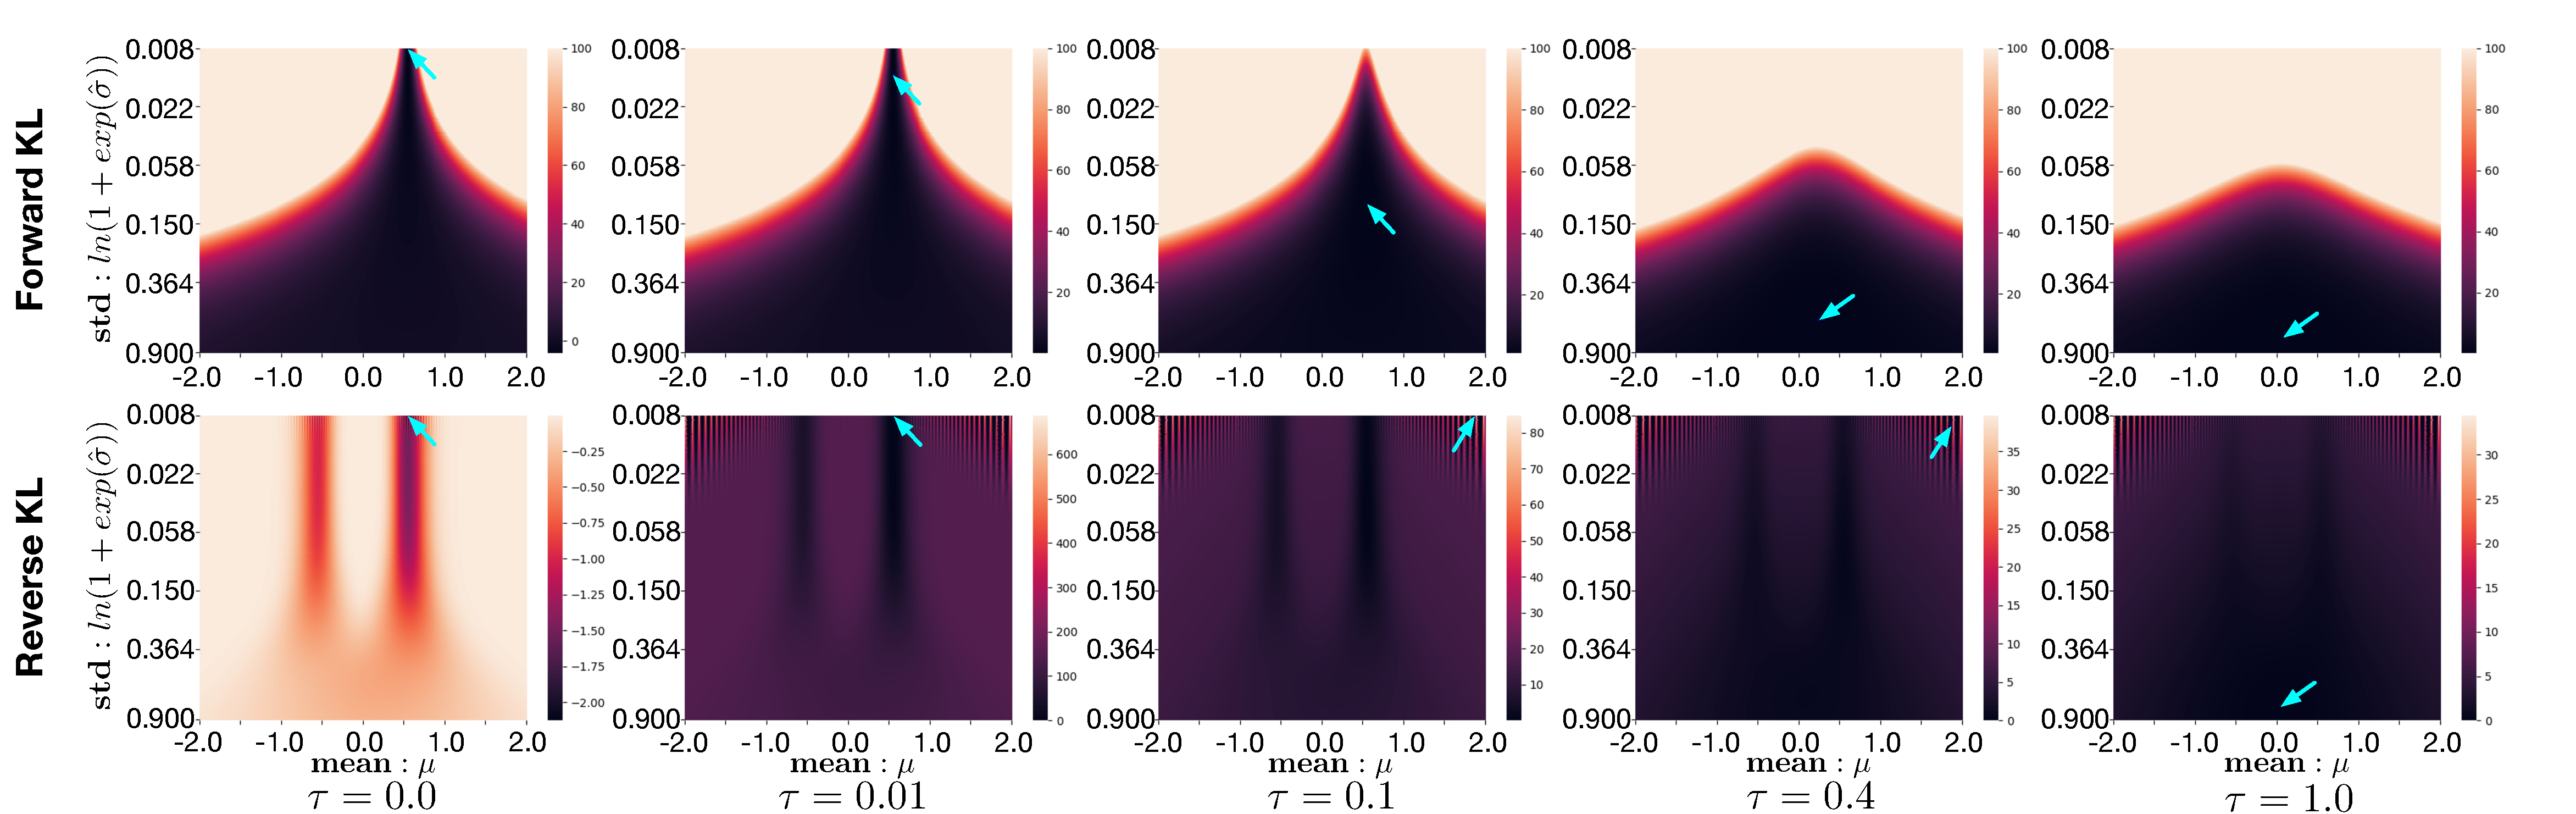
\includegraphics[width=0.99\columnwidth]{figs/bandit/trueQ/heatmaps/heatmap_combined_reduced_pts.pdf}
    \caption{KL loss over mean and standard deviation across temperature using the Gaussian policy with 128 numerical integration points. }
    \label{fig:bandit-heatmap-reduced-pts}
\end{figure}

\begin{figure}
    \centering
    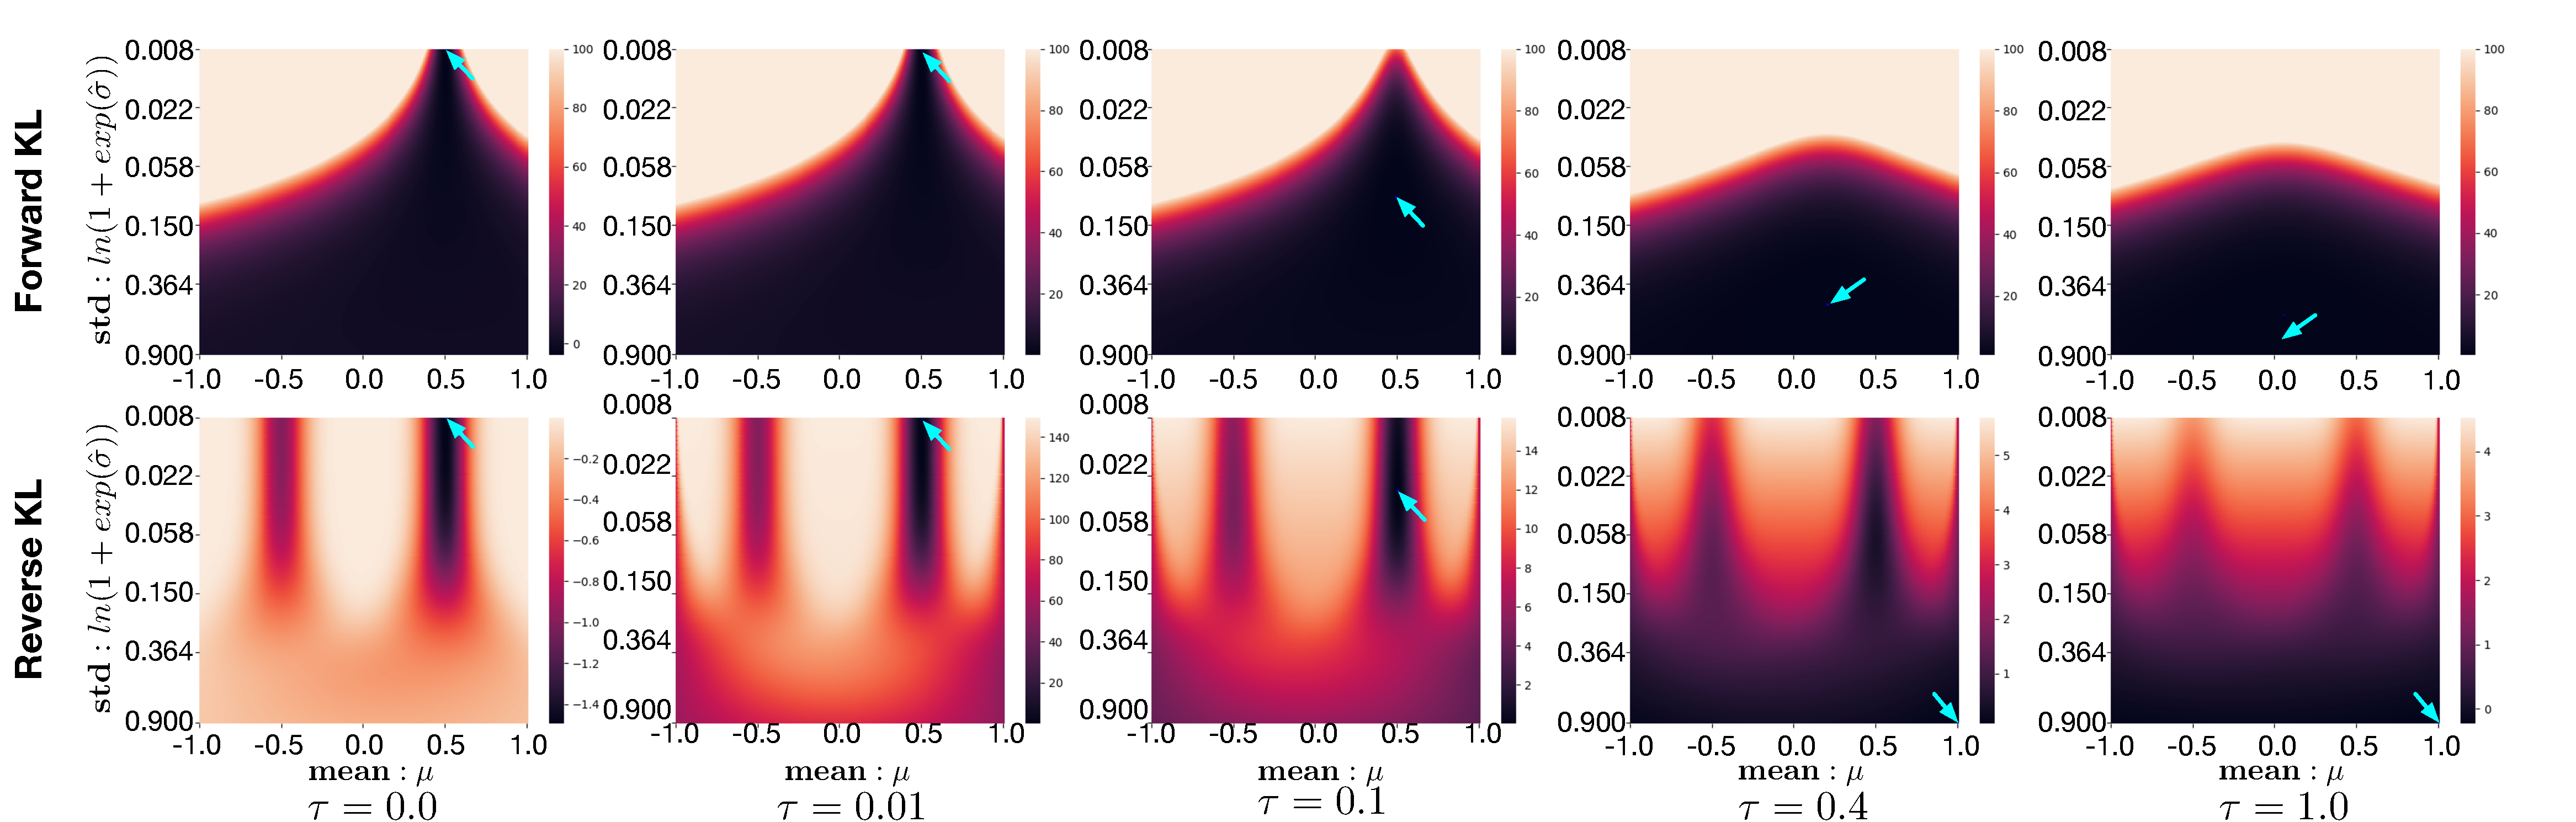
\includegraphics[width=0.99\columnwidth]{figs/bandit/trueQ/heatmaps/heatmap_non_tanh_combined.pdf}
    \caption{KL loss over mean and standard deviation across temperature using the Gaussian policy without $\tanh$ transformation. Note that the displayed mean range is $[-1,1]$. Different from the previous heatmap, optima are now located at $a=-0.5, 0.5$.  FKL loss has been upper-bounded for better visualization of minima.}
    \label{fig:bandit-heatmap-non-tanh}
\end{figure}

\subsection{Continuous Bandits - Optimization Path}
Here, we include additional plots for the optimization behaviour of iterates in the continuous bandit. We also include additional summary statistics for the iterates. 

% \begin{figure}[!ht]
%   \centering
%   \begin{subfigure}[b]{0.4\linewidth}
%     \centering
%     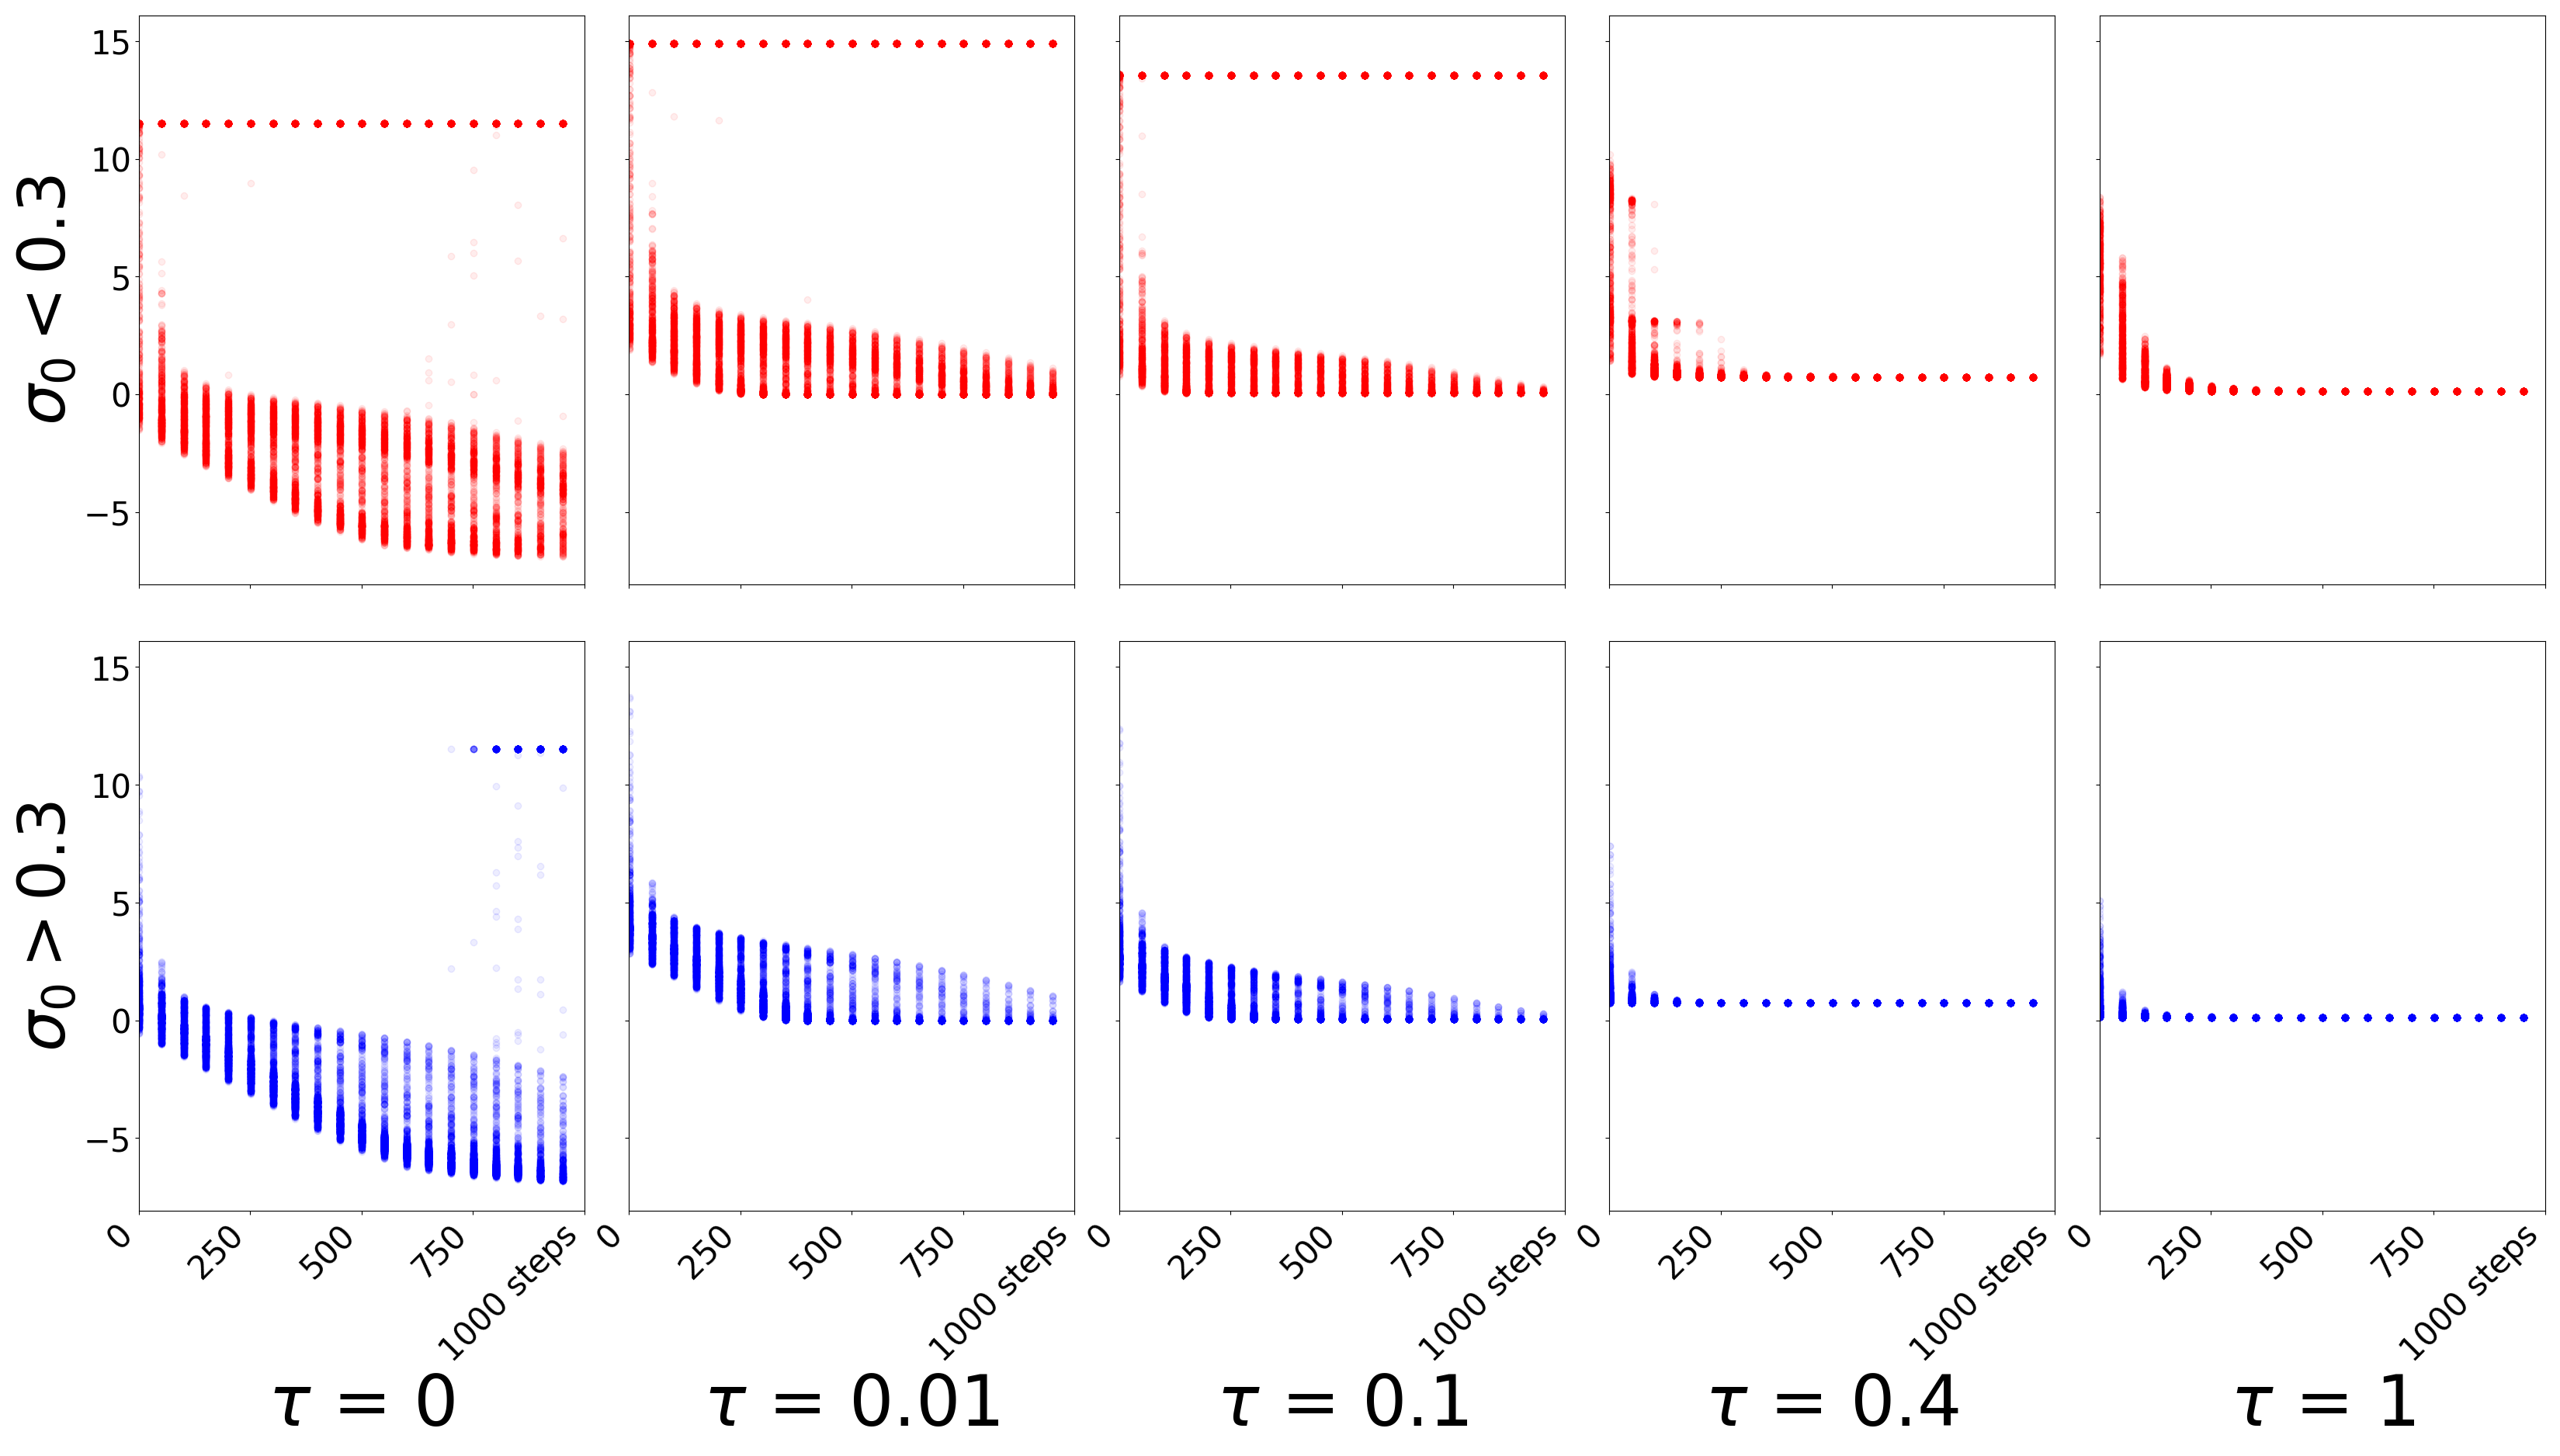
\includegraphics[width=1\columnwidth]{figs/bandit/notlearnQ/modes=1/adam/loss_forward_optim=adam_modes=1_lr=0.01.png}
%     \caption{Forward KL, Adam.}
%     \label{fig:bandit-loss-forward-adam}
%   \end{subfigure}%
%   \begin{subfigure}[b]{0.4\linewidth}
%     \centering
%     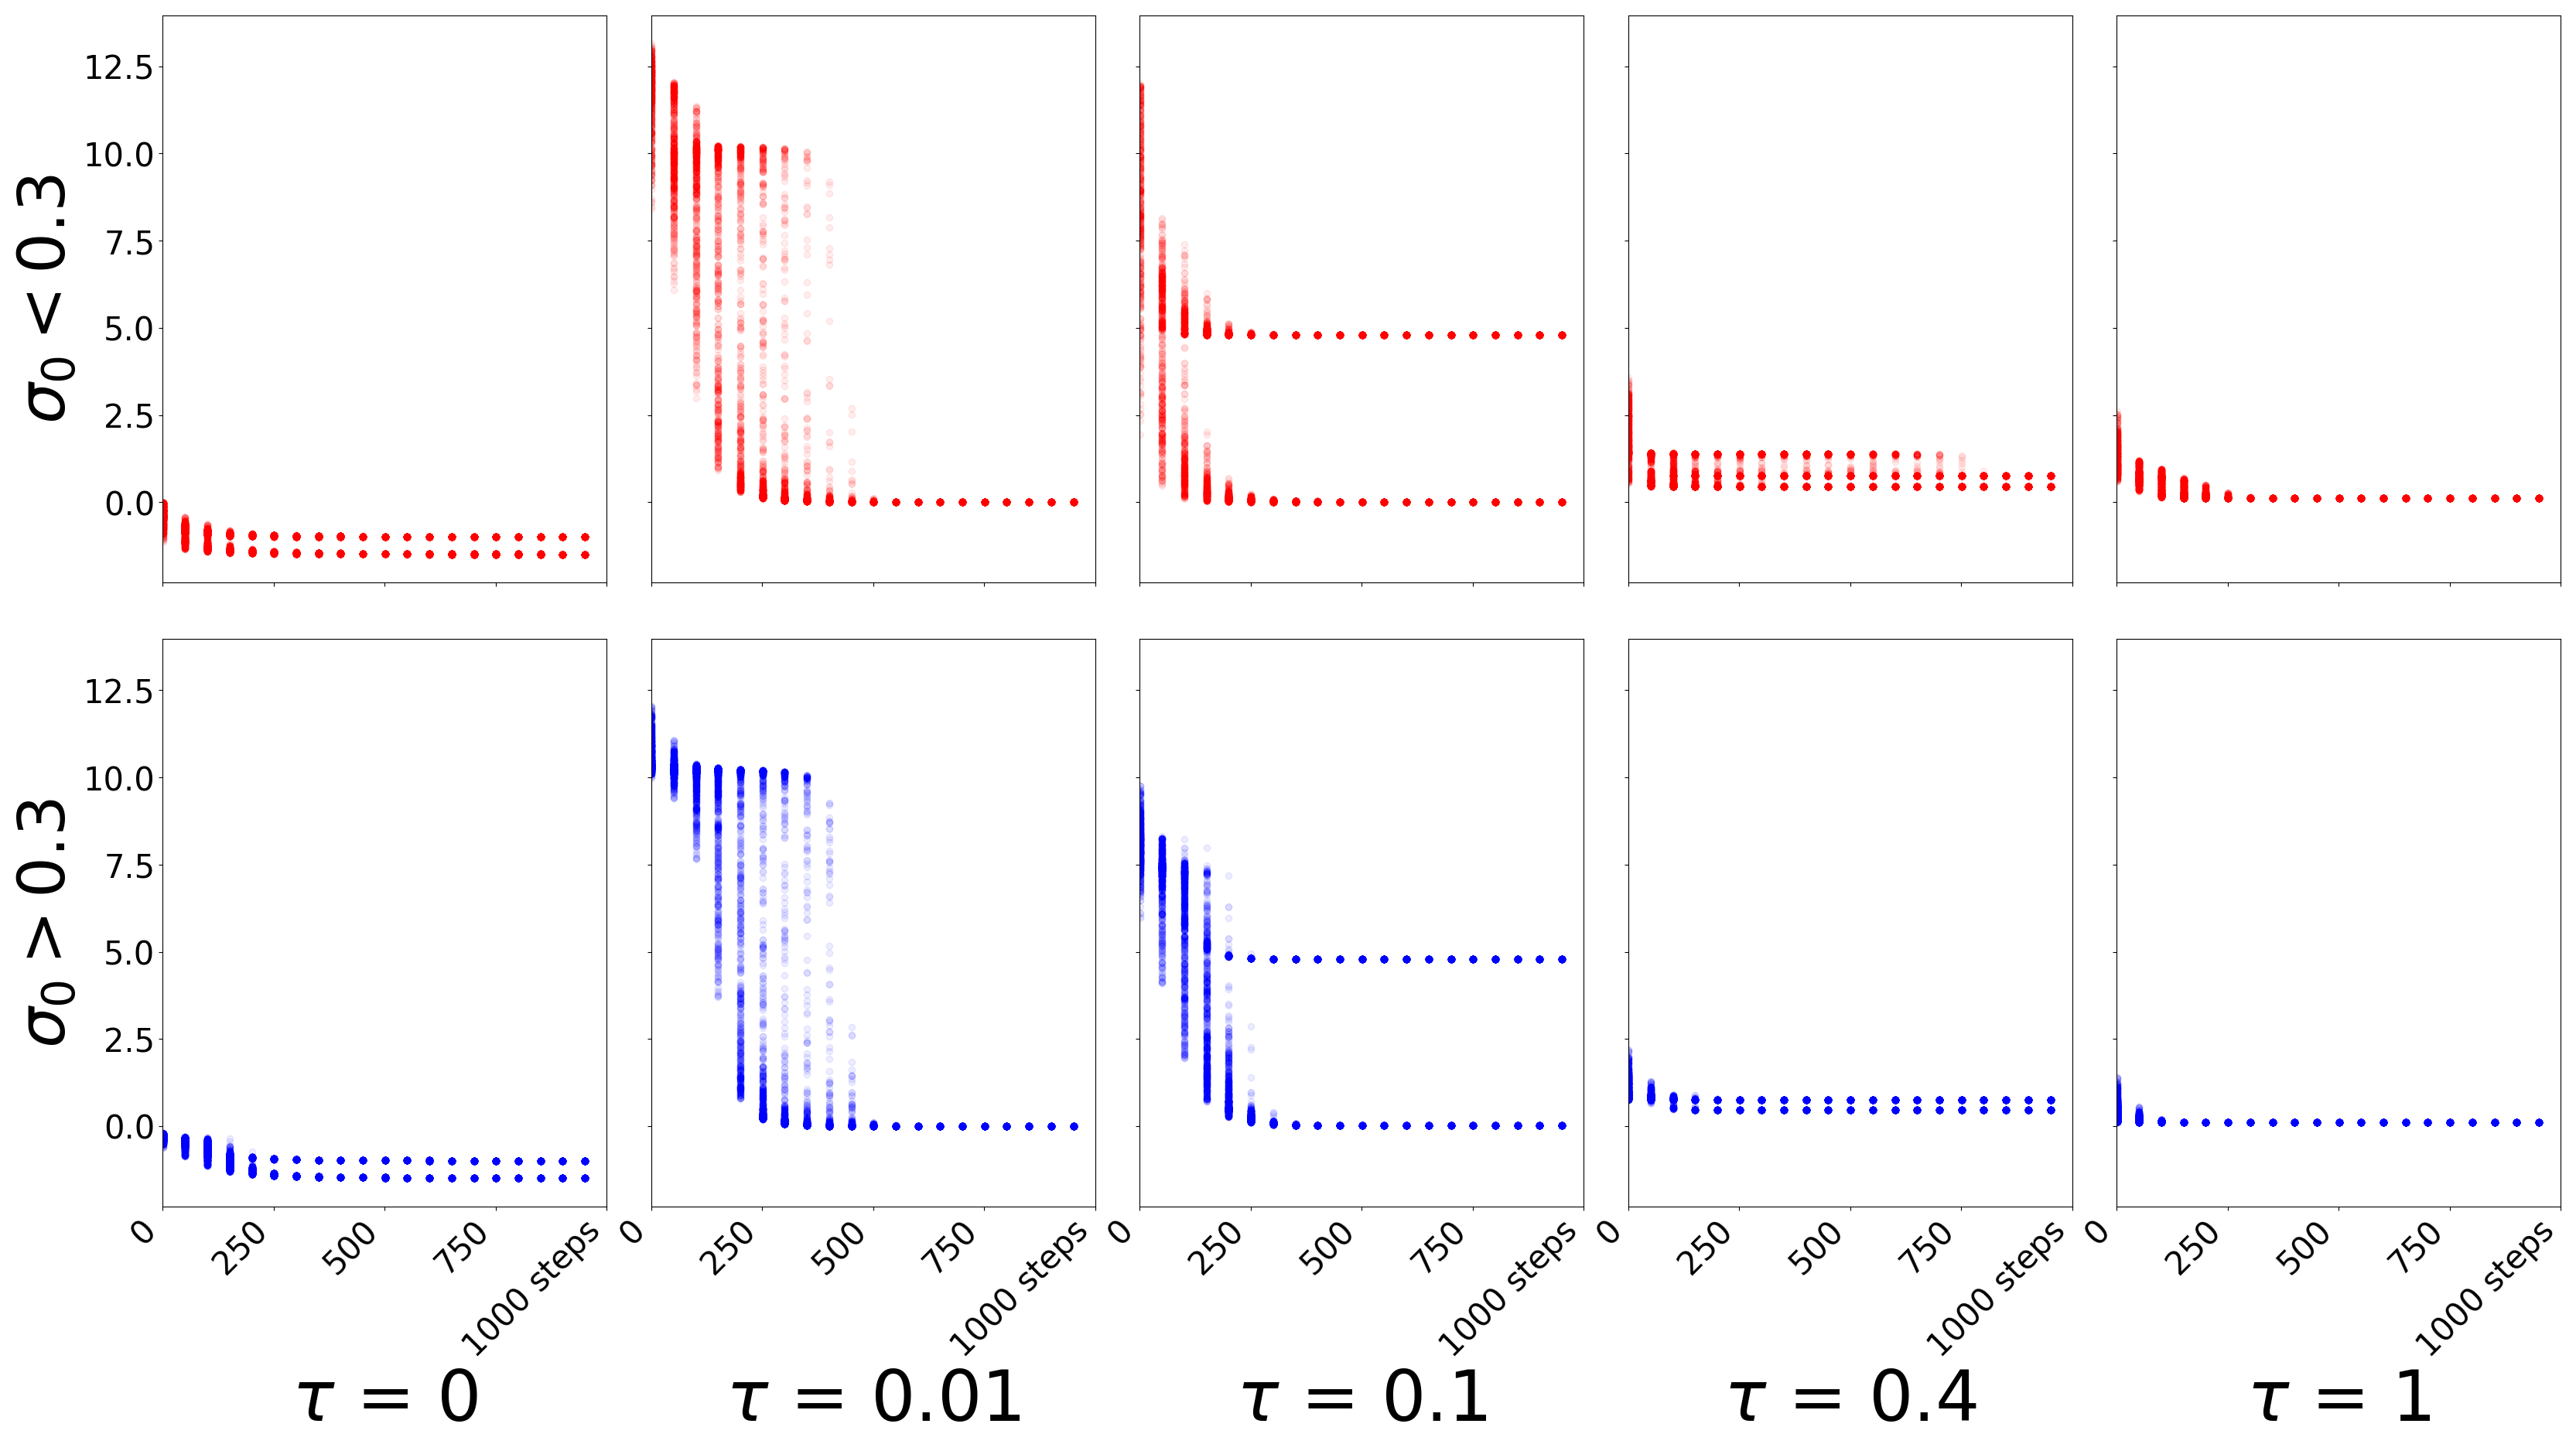
\includegraphics[width=1\columnwidth]{figs/bandit/notlearnQ/modes=1/adam/loss_reverse_optim=adam_modes=1_lr=0.01.png}
%     \caption{Reverse KL, Adam. }
%     \label{fig:bandit-loss-reverse-adam}
%   \end{subfigure}
  
%   \begin{subfigure}[b]{0.4\linewidth}
%     \centering
%     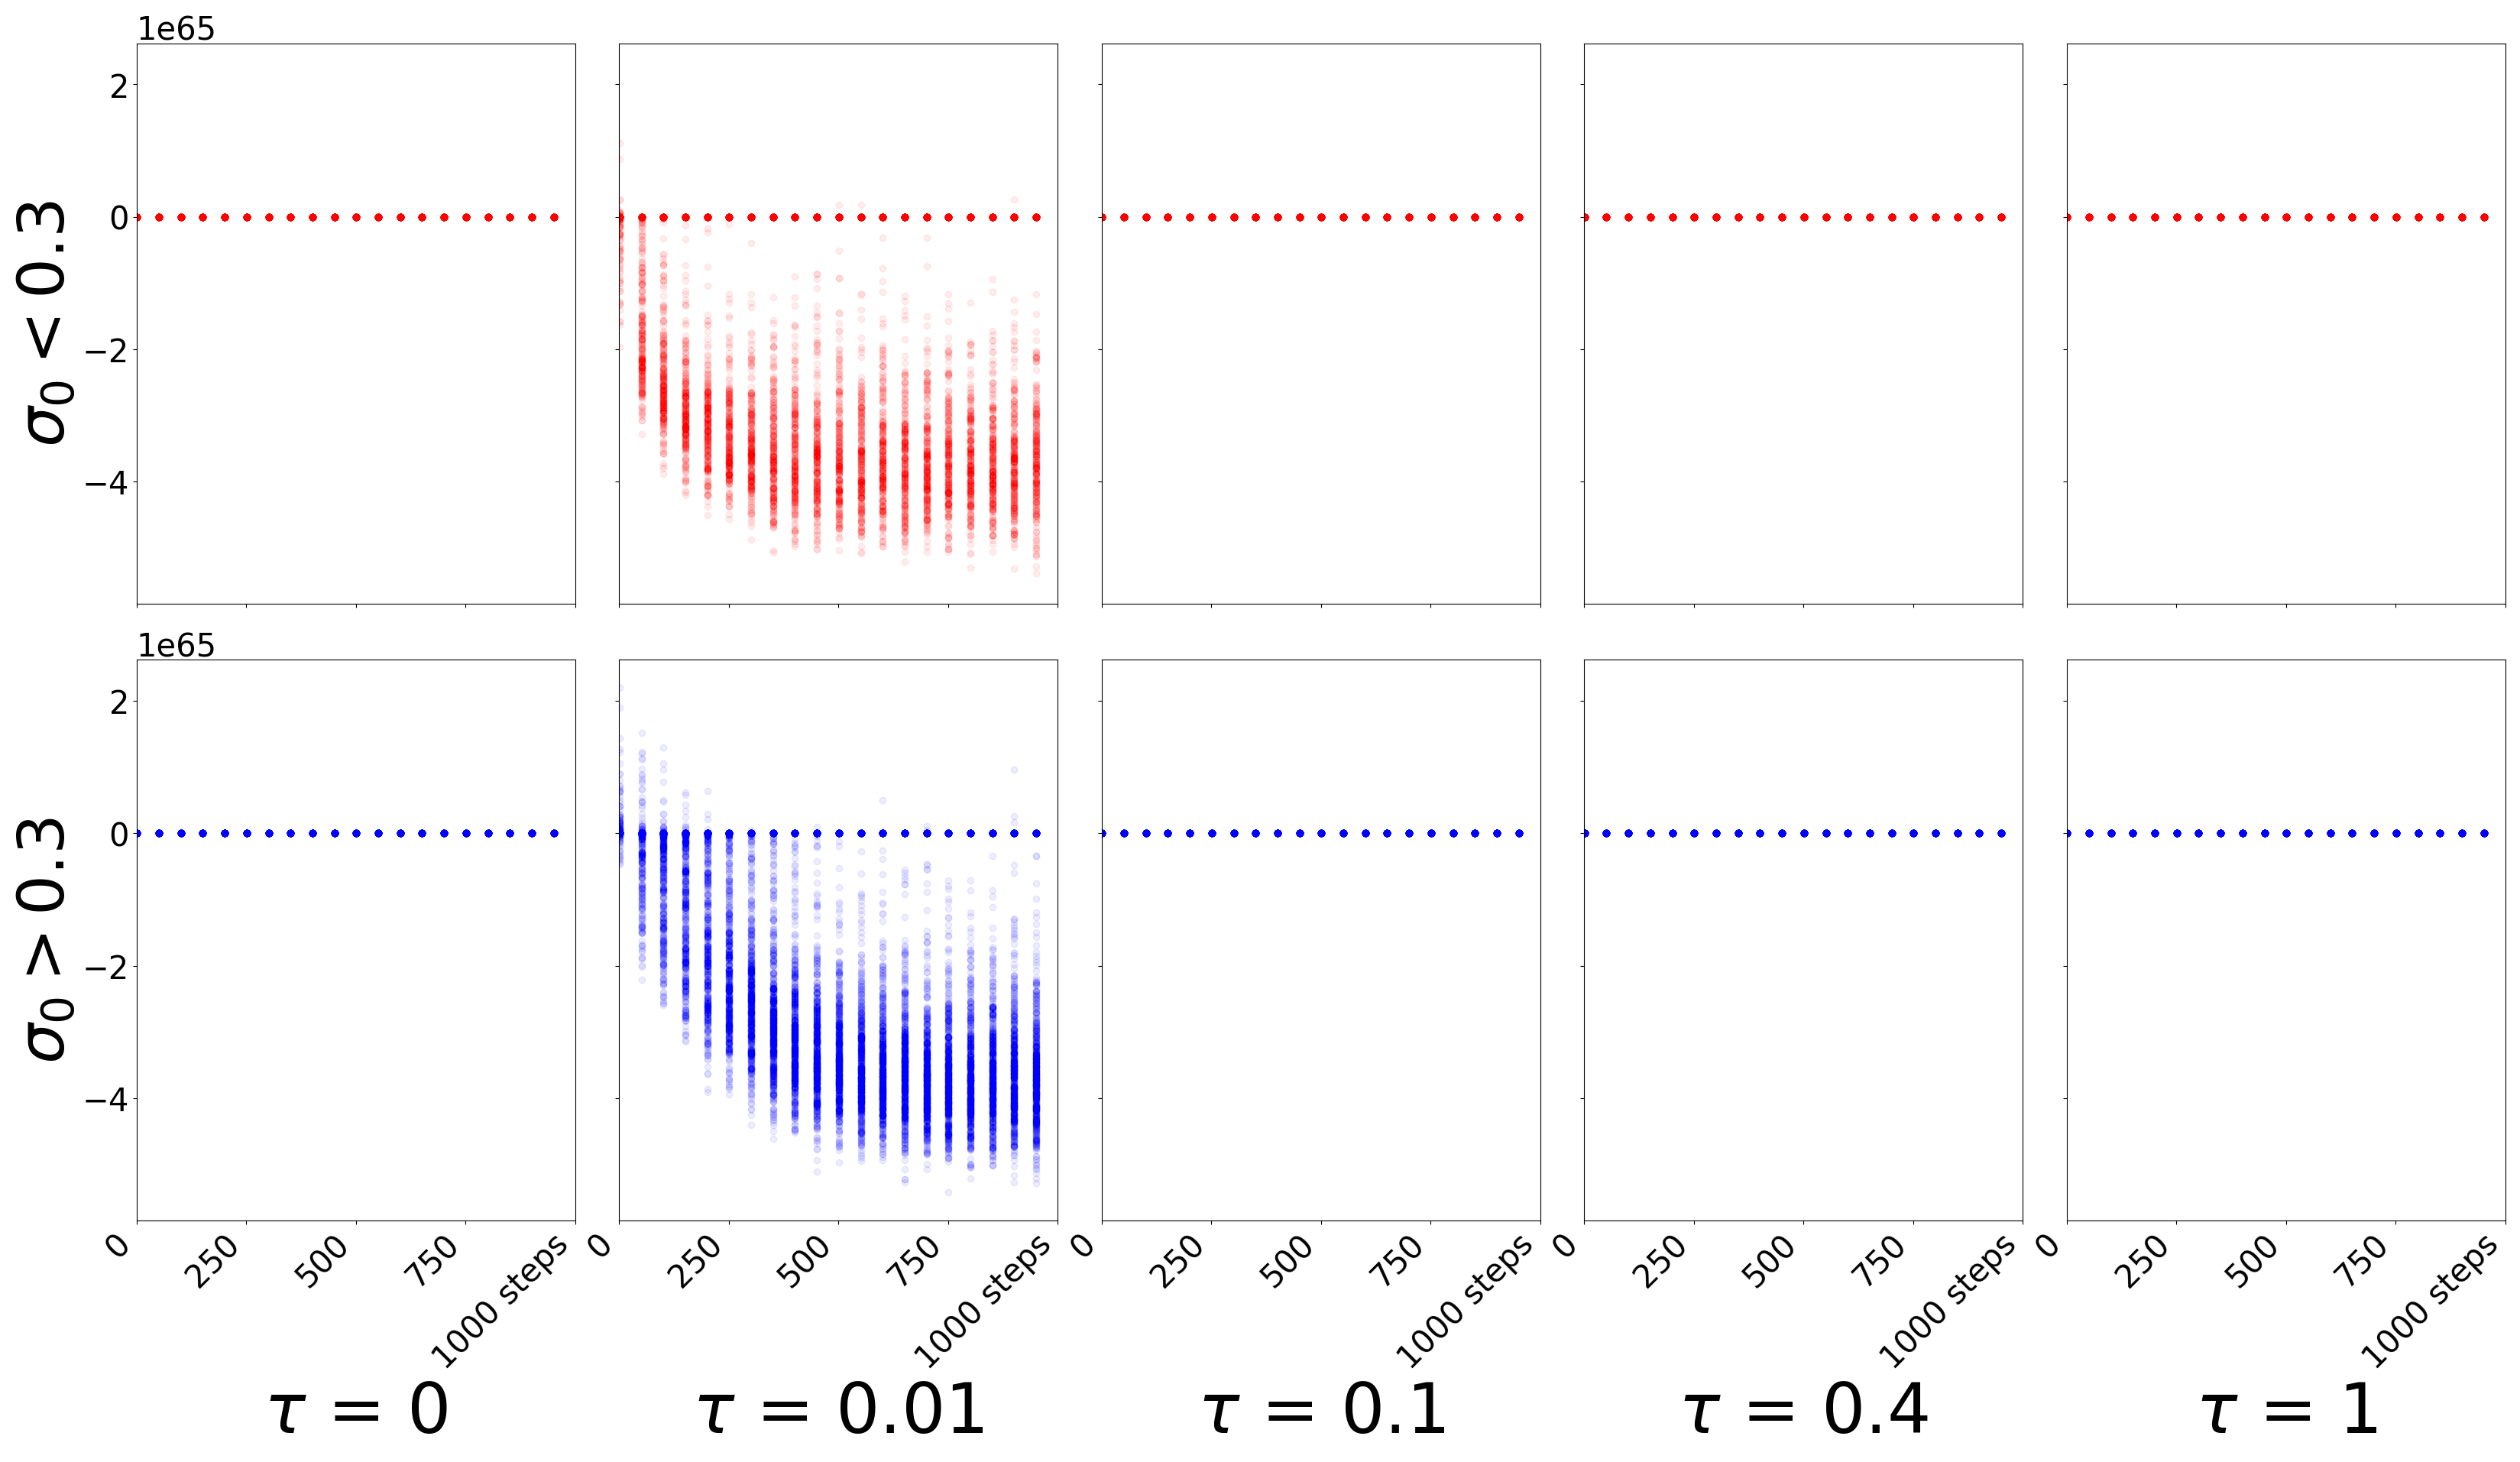
\includegraphics[width=1\columnwidth]{figs/bandit/notlearnQ/modes=1/rmsprop/loss_forward_optim=rmsprop_modes=1_lr=0.01.png}
%     \caption{Forward KL, RMSprop.}
%     \label{fig:bandit-loss-forward-rmsprop}
%   \end{subfigure}%
%   \begin{subfigure}[b]{0.4\linewidth}
%     \centering
%     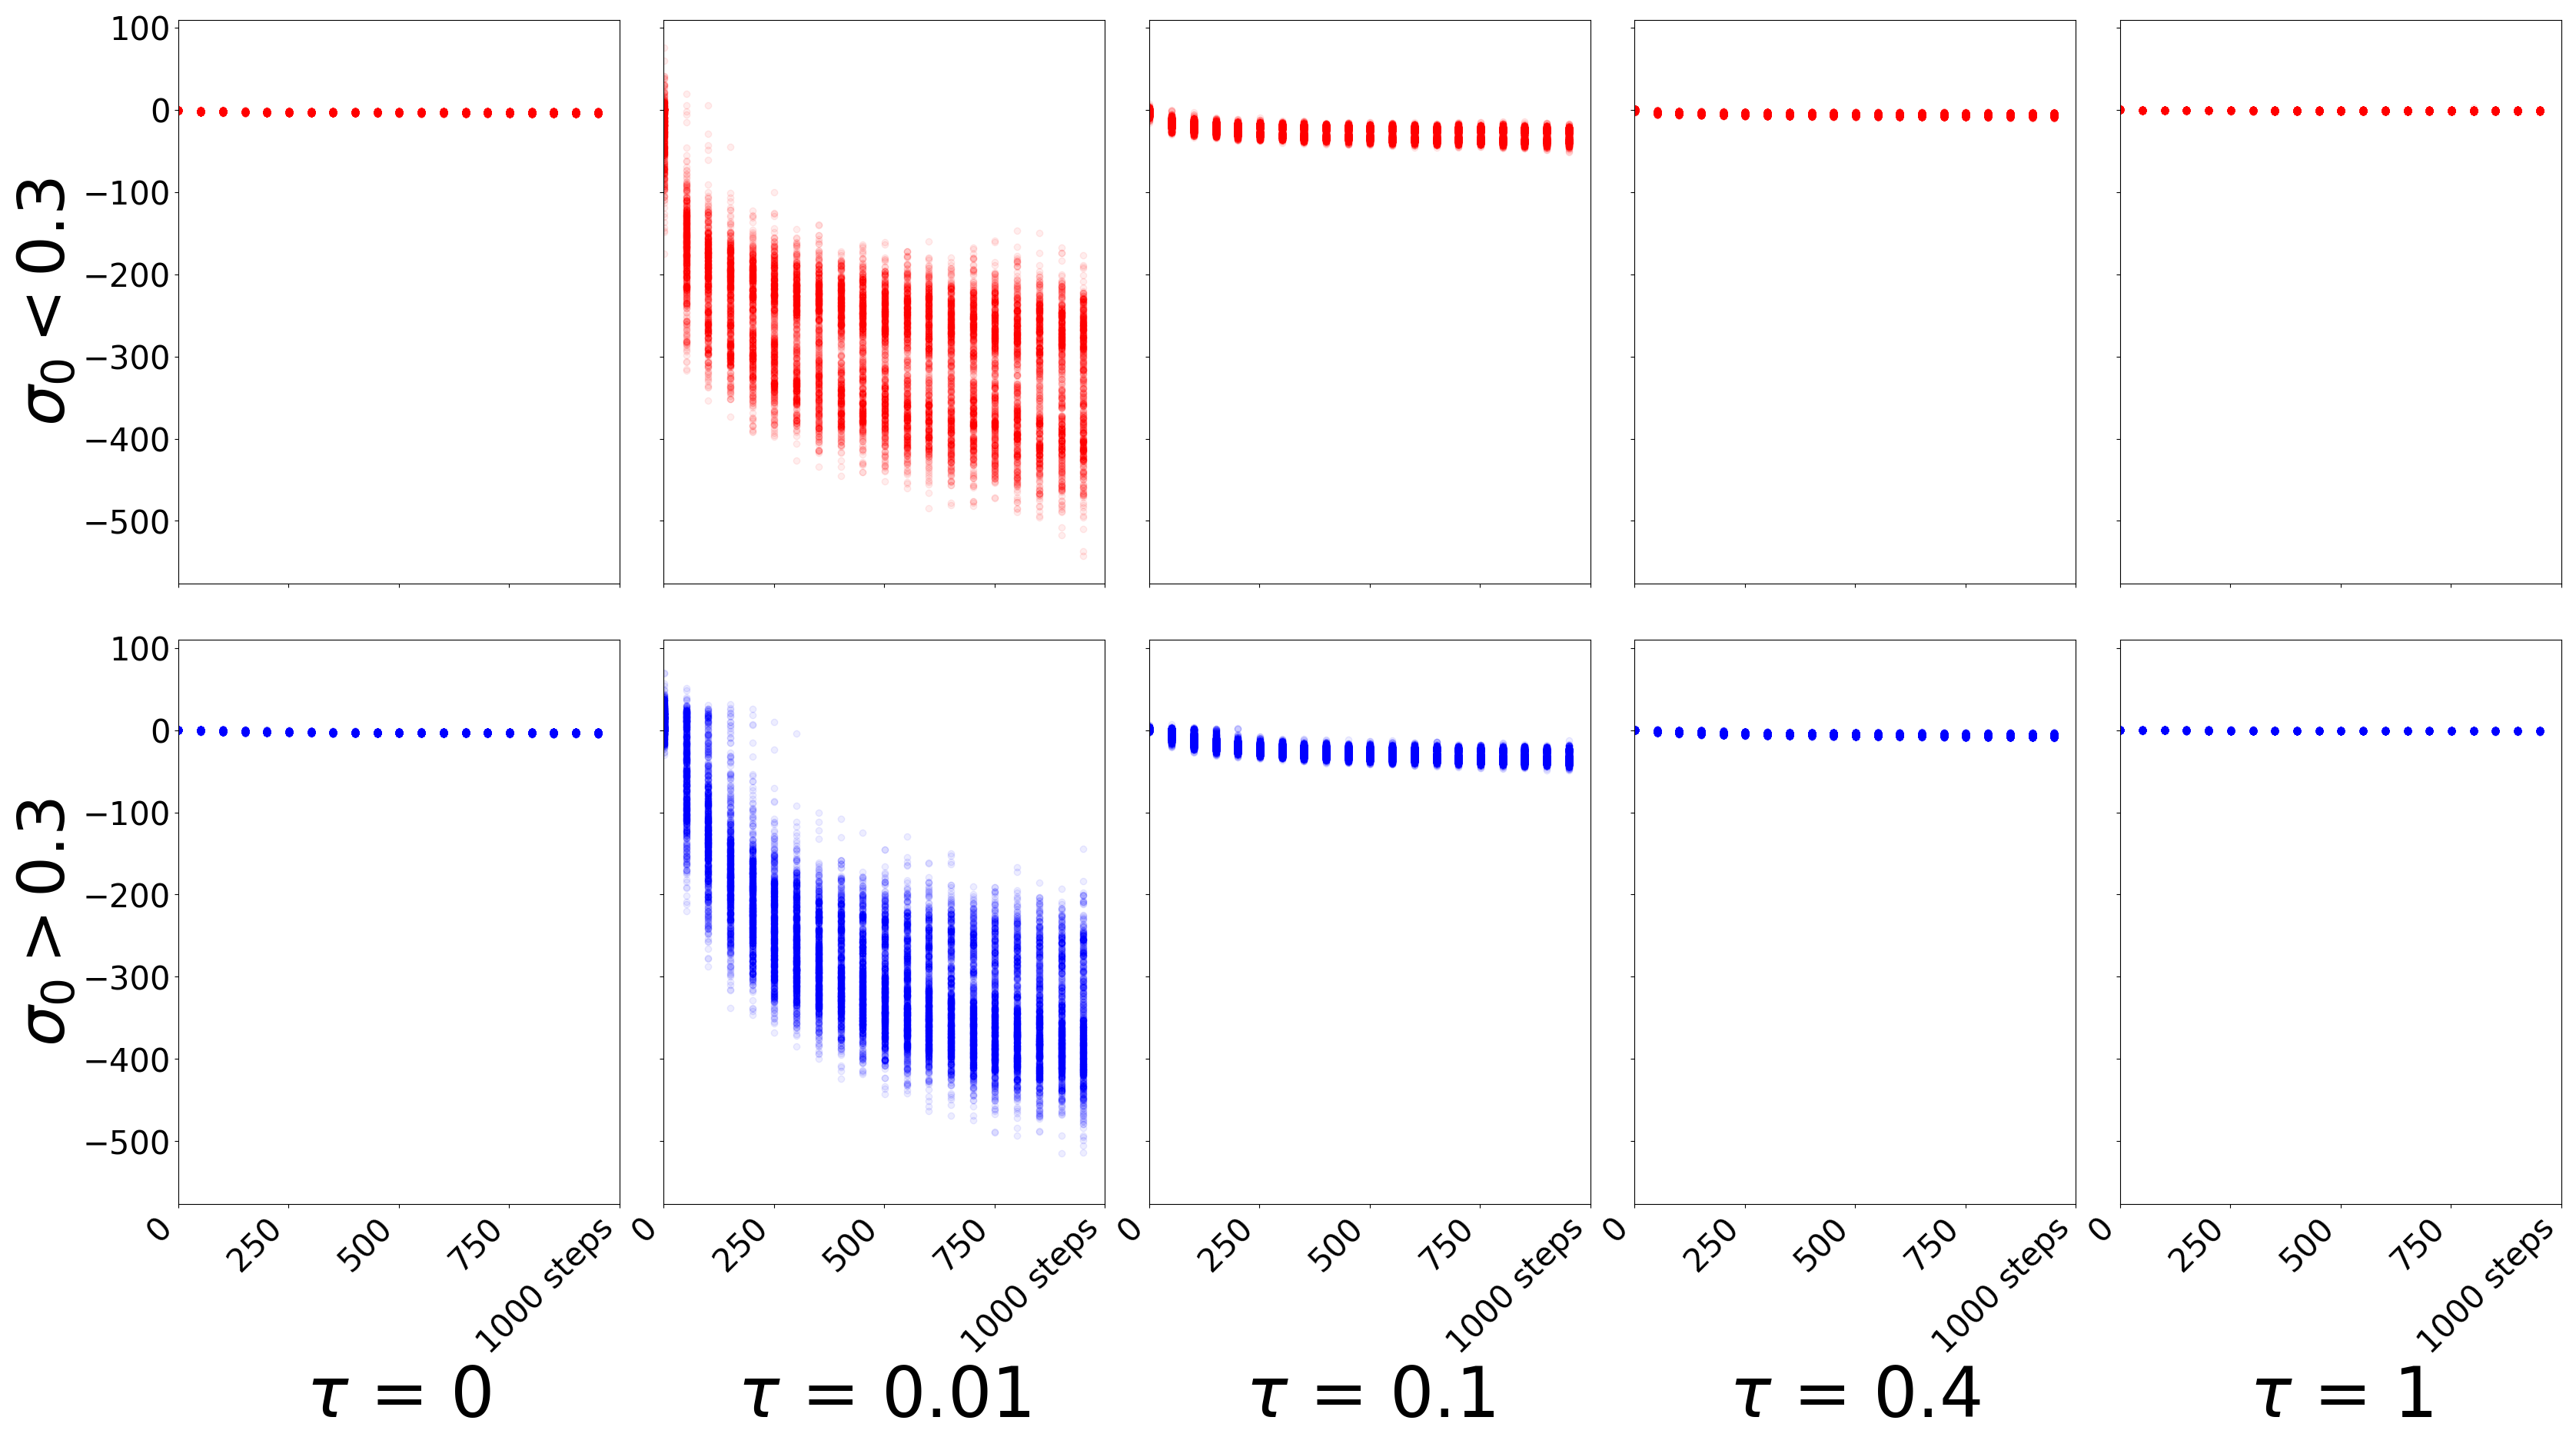
\includegraphics[width=1\columnwidth]{figs/bandit/notlearnQ/modes=1/rmsprop/loss_reverse_optim=rmsprop_modes=1_lr=0.01.png}
%     \caption{Reverse KL, RMSprop.}
%     \label{fig:bandit-loss-reverse-rmsprop}
%   \end{subfigure}
  
%   \begin{subfigure}[b]{0.4\linewidth}
%     \centering
%     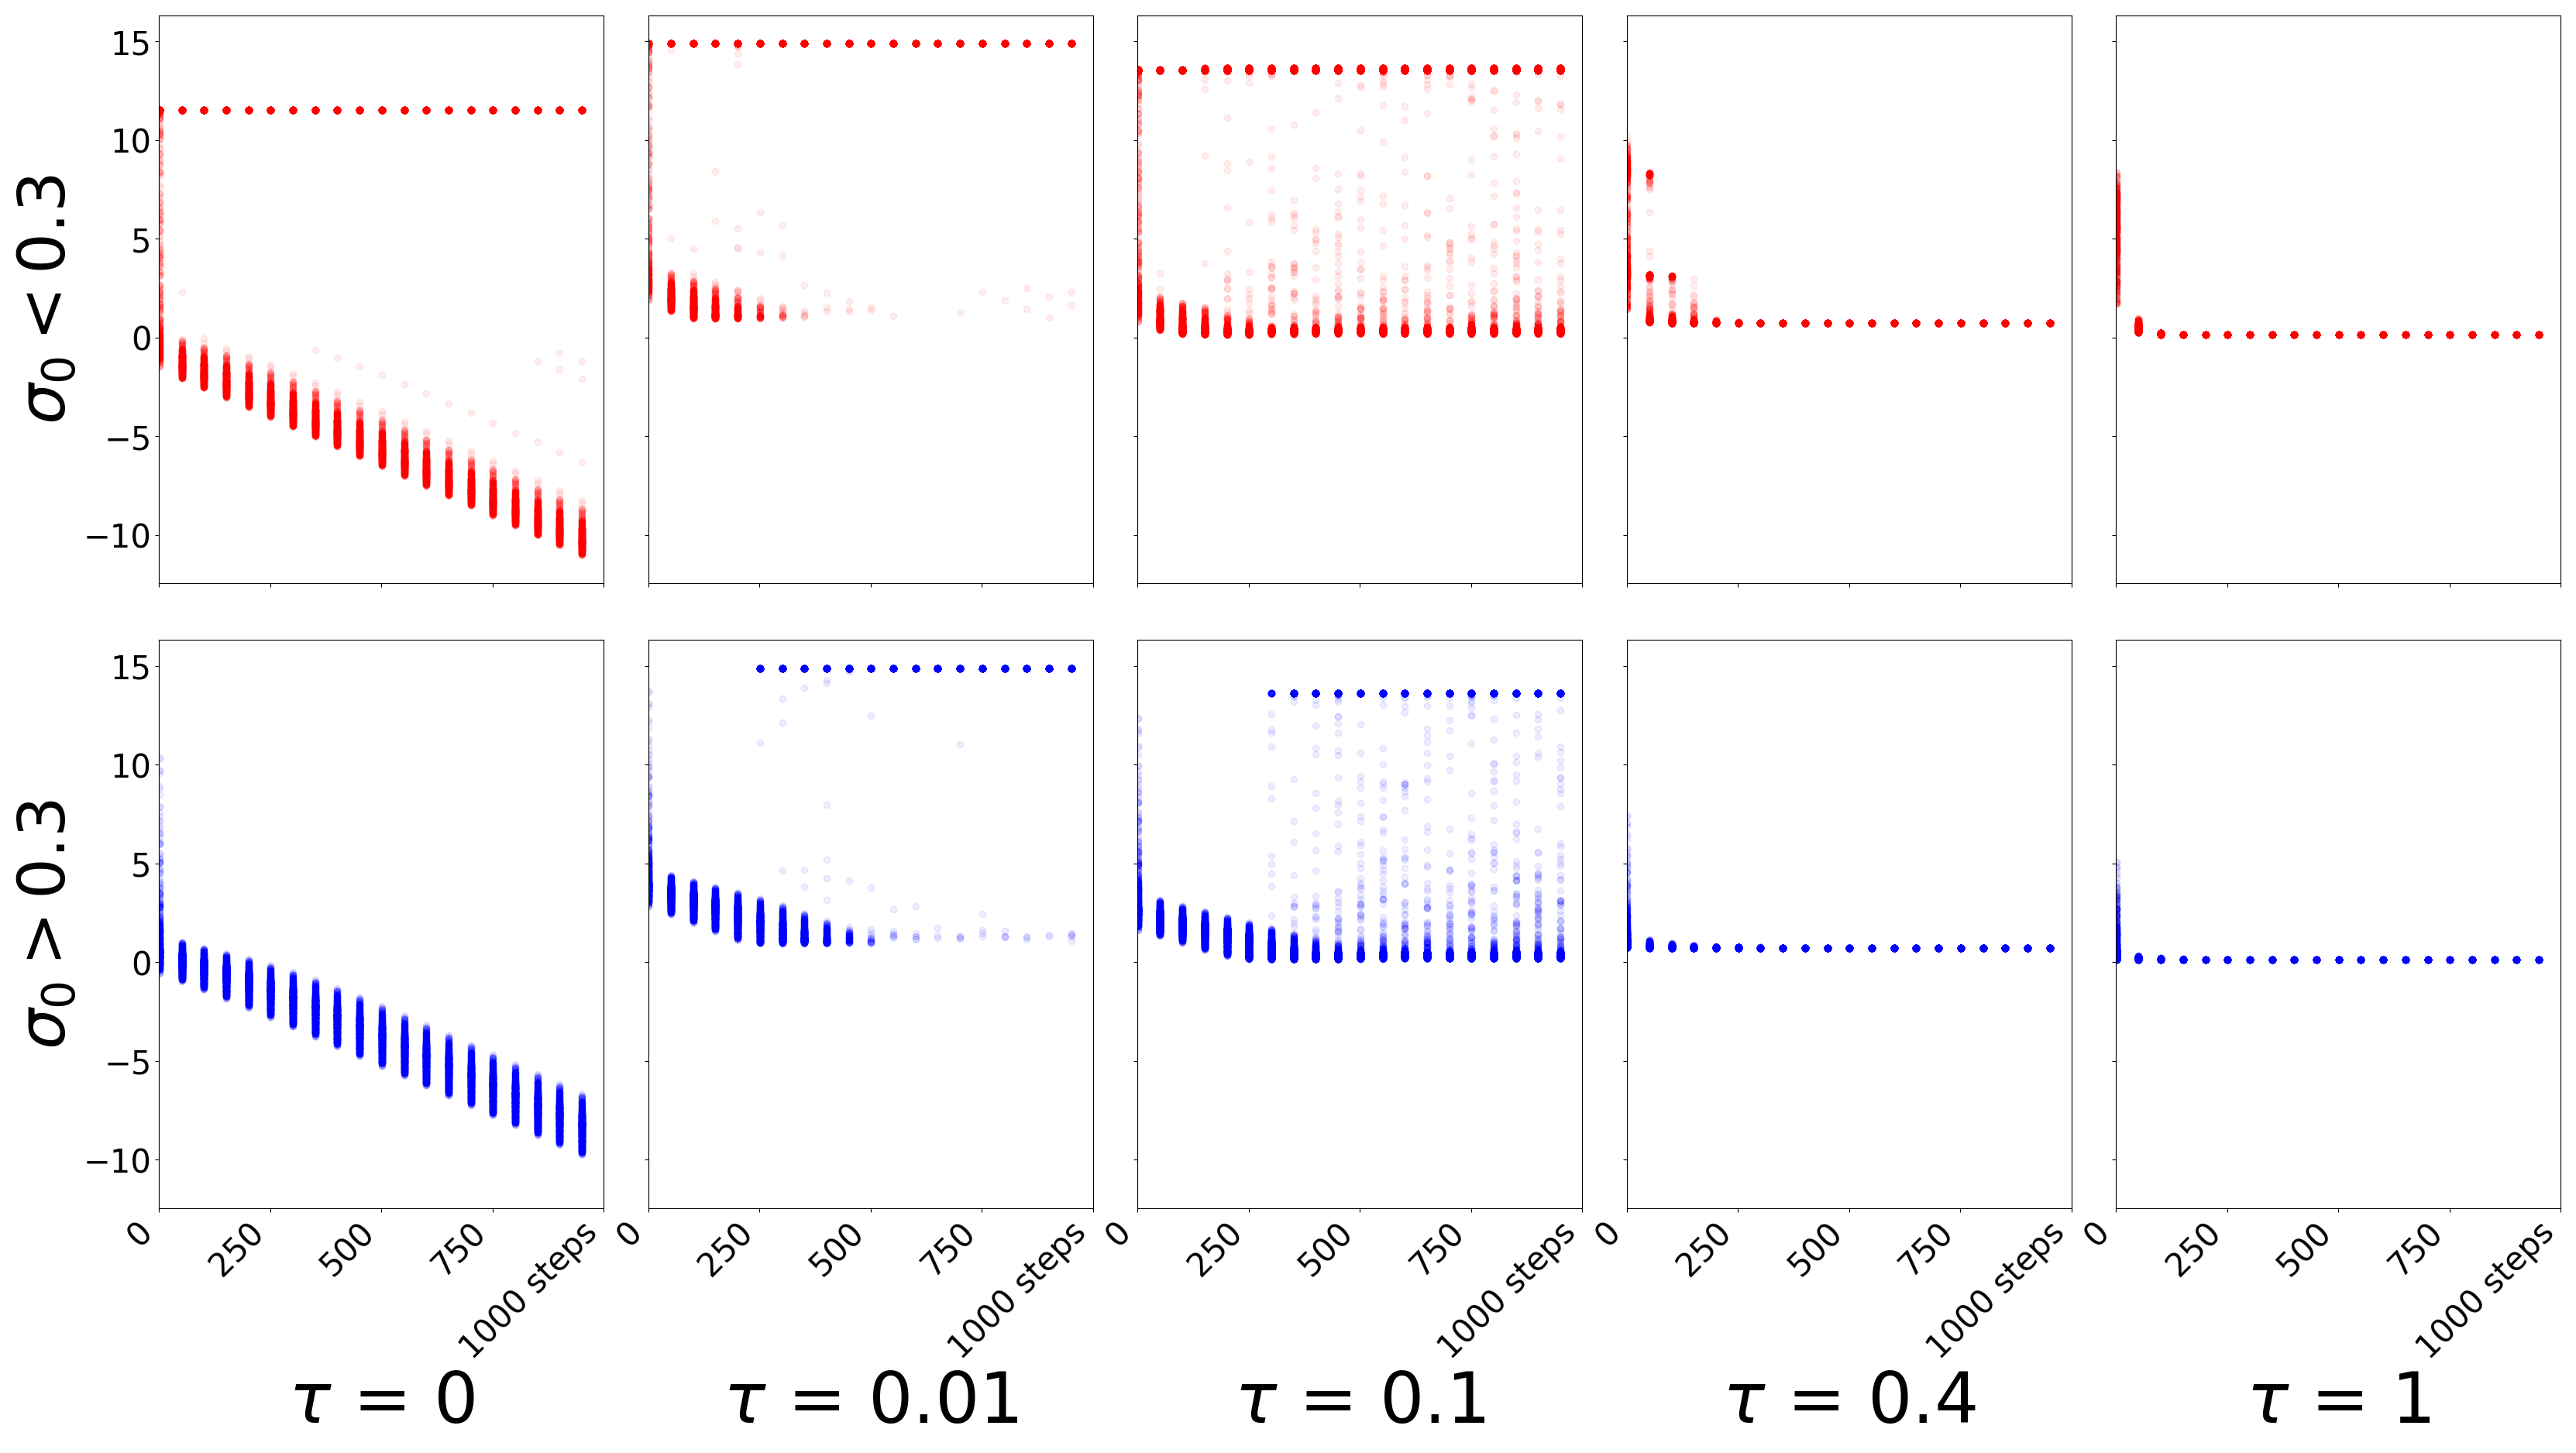
\includegraphics[width=1\columnwidth]{figs/bandit/notlearnQ/modes=1/sgd/loss_forward_optim=sgd_modes=1_lr=0.01.png}
%     \caption{Forward KL, SGD.}
%     \label{fig:bandit-loss-forward-sgd}
%   \end{subfigure}%
%   \begin{subfigure}[b]{0.4\linewidth}
%     \centering
%     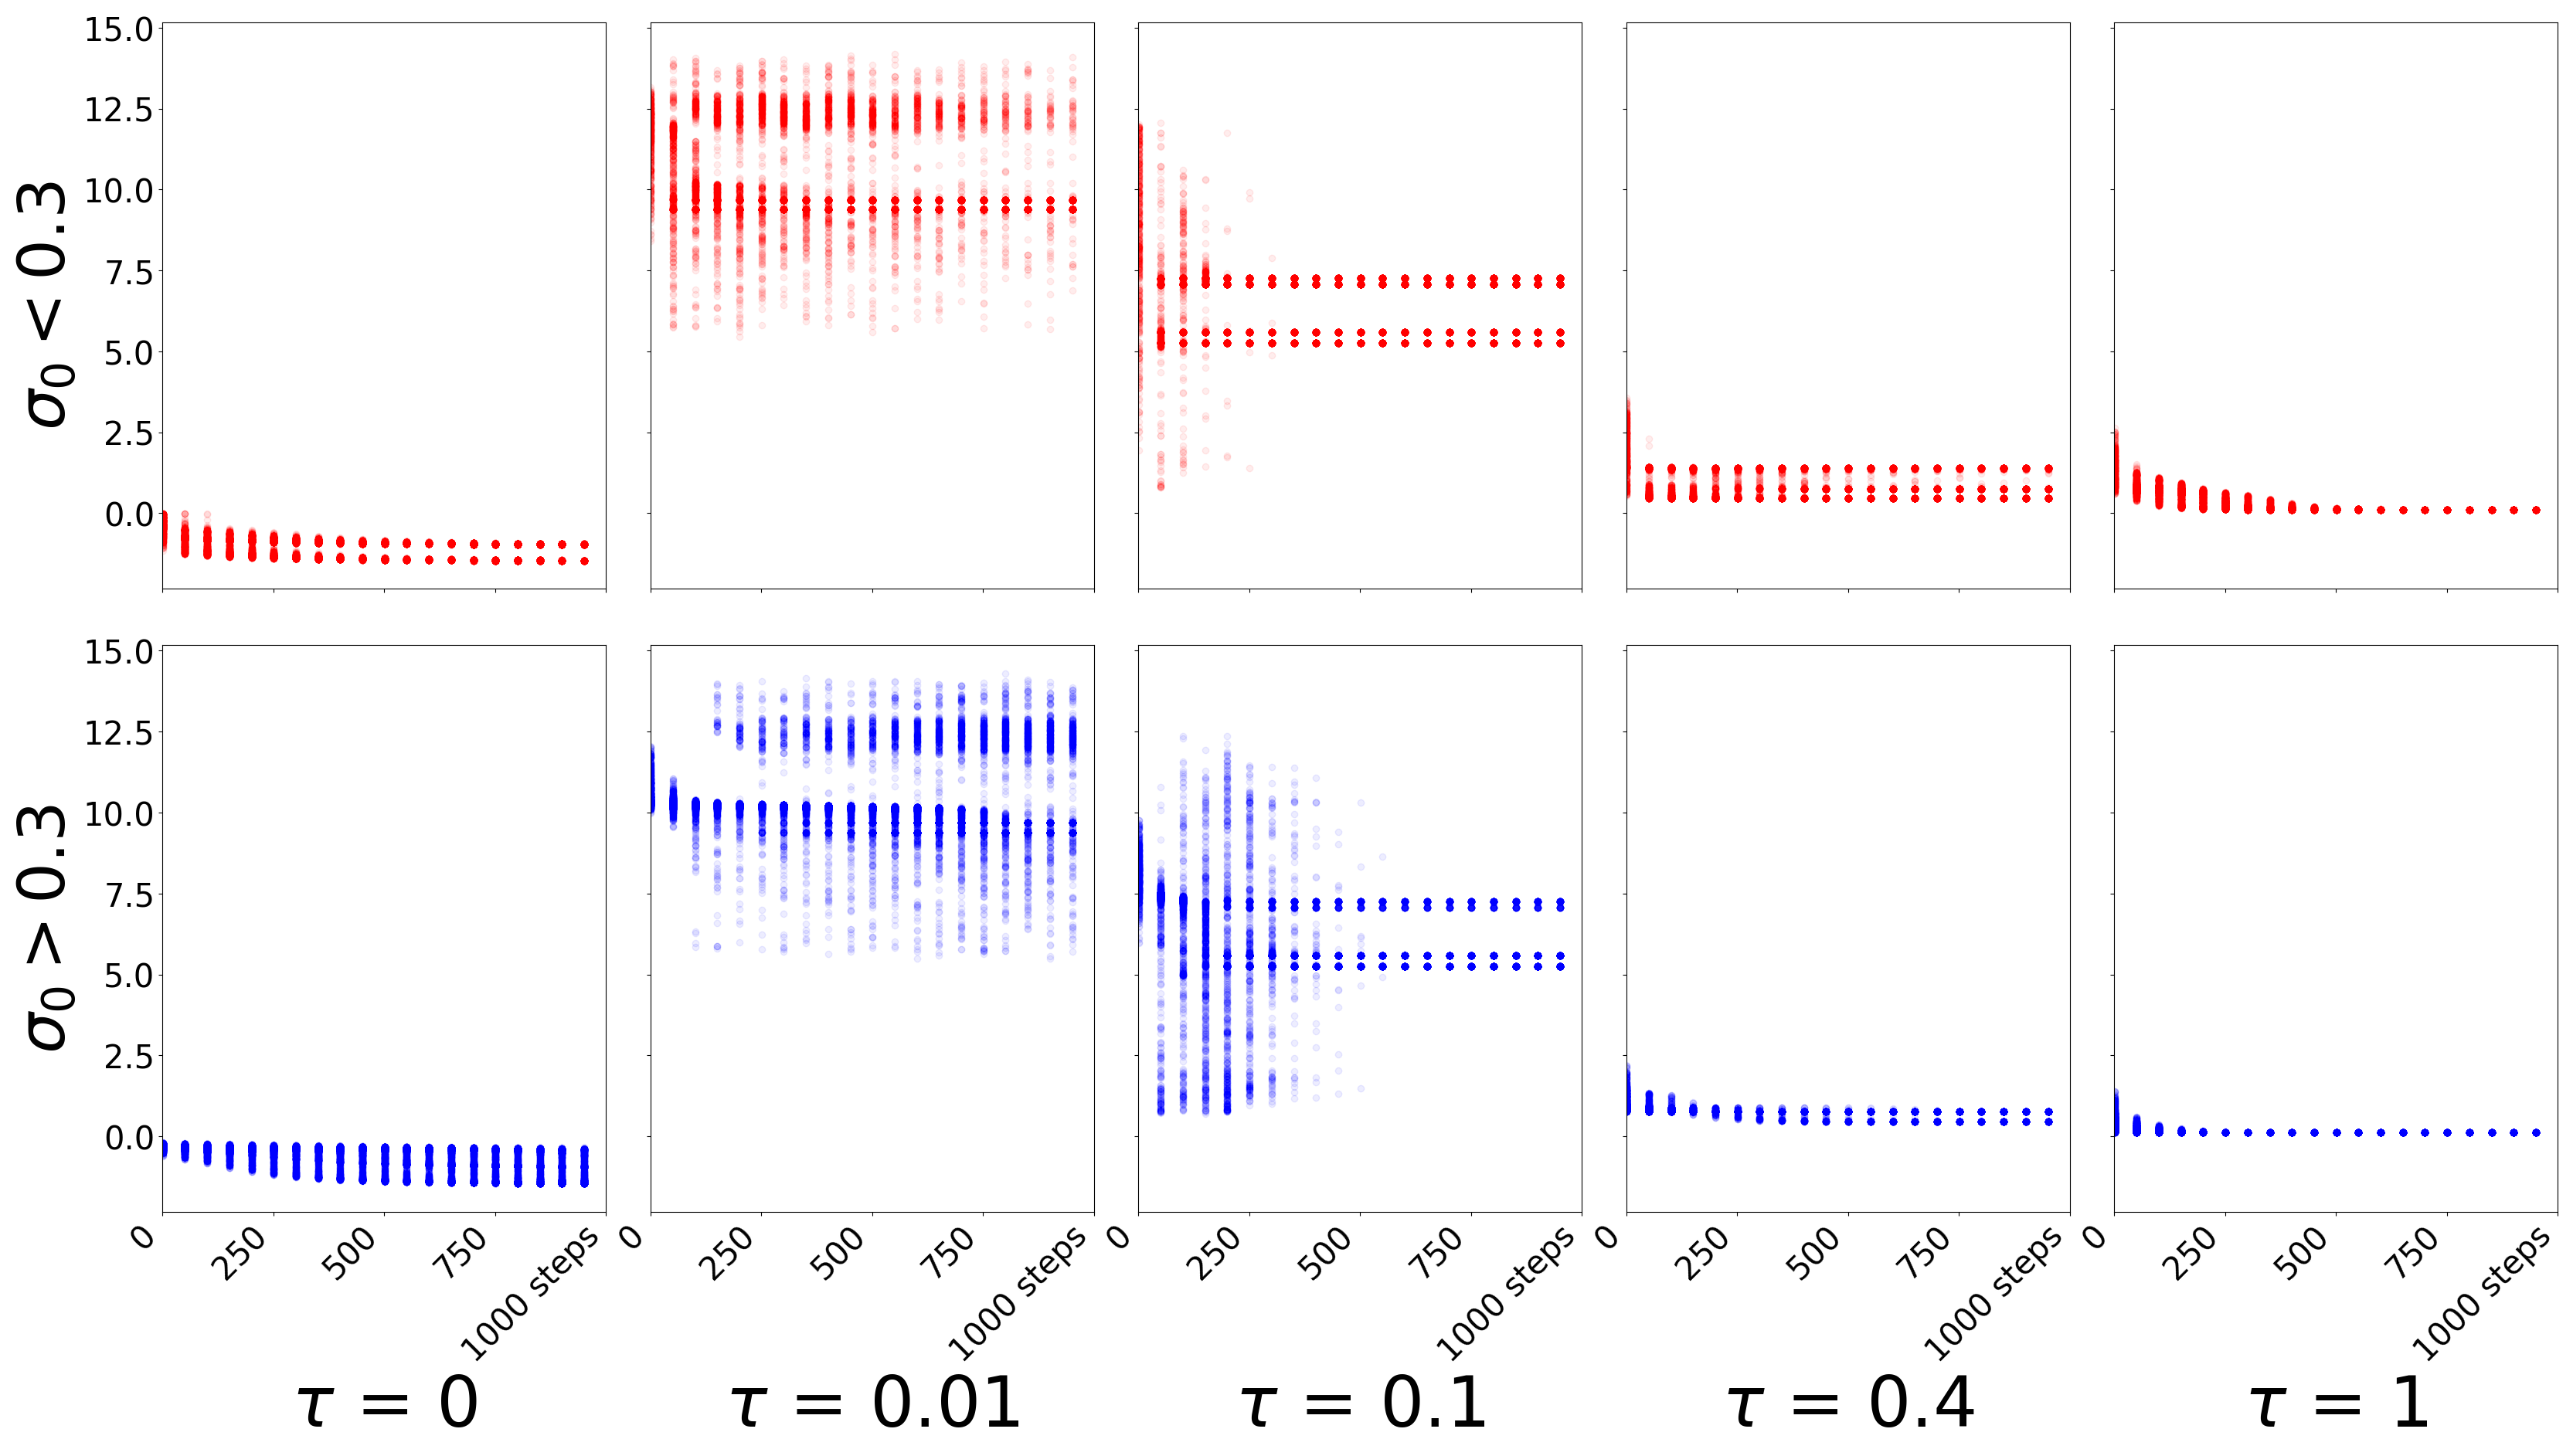
\includegraphics[width=1\columnwidth]{figs/bandit/notlearnQ/modes=1/sgd/loss_reverse_optim=sgd_modes=1_lr=0.01.png}
%     \caption{Reverse KL, SGD.}
%     \label{fig:bandit-loss-reverse-sgd}
%   \end{subfigure}
%   \caption{Loss over time with unimodal policy. }
% \end{figure}

\begin{figure}[!ht]
  \centering
  \begin{subfigure}[b]{0.4\linewidth}
    \centering
    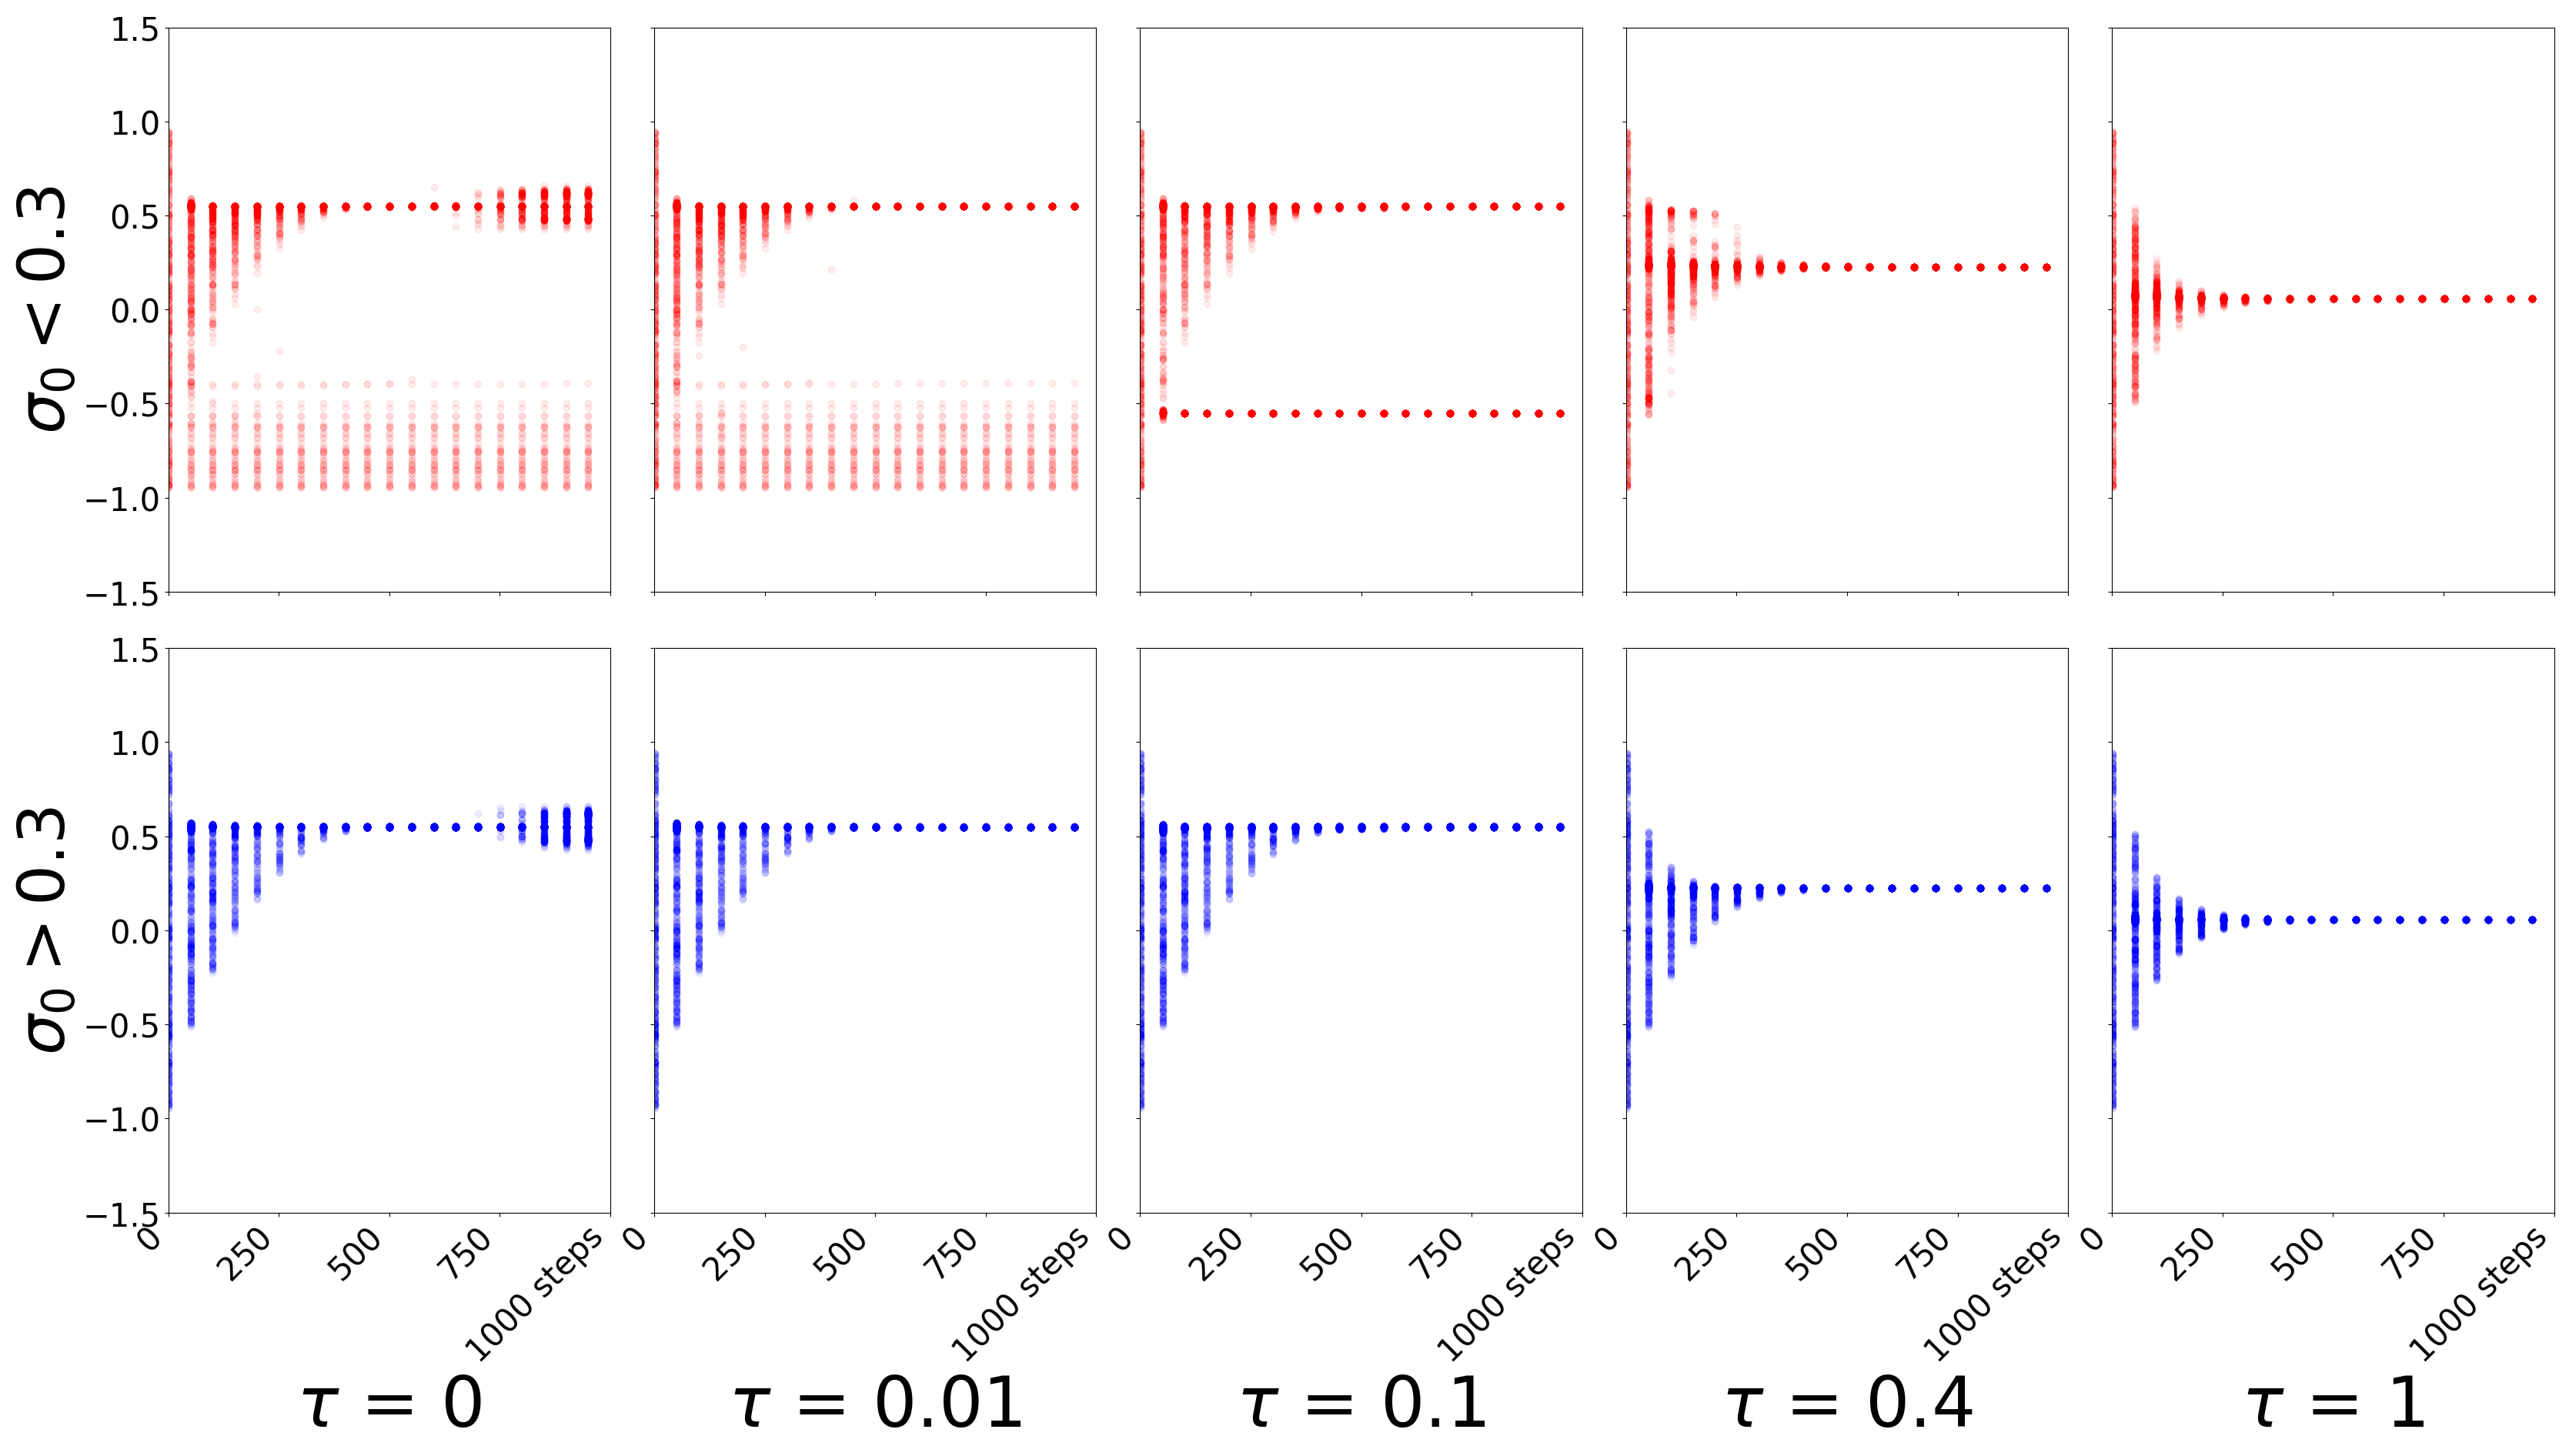
\includegraphics[width=1\columnwidth]{figs/bandit/notlearnQ/modes=1/adam/mean_forward_optim=adam_modes=1_lr=0.01.png}
    \caption{Forward KL, Adam.}
    \label{fig:bandit-mean-forward-adam}
  \end{subfigure}%
  \begin{subfigure}[b]{0.4\linewidth}
    \centering
    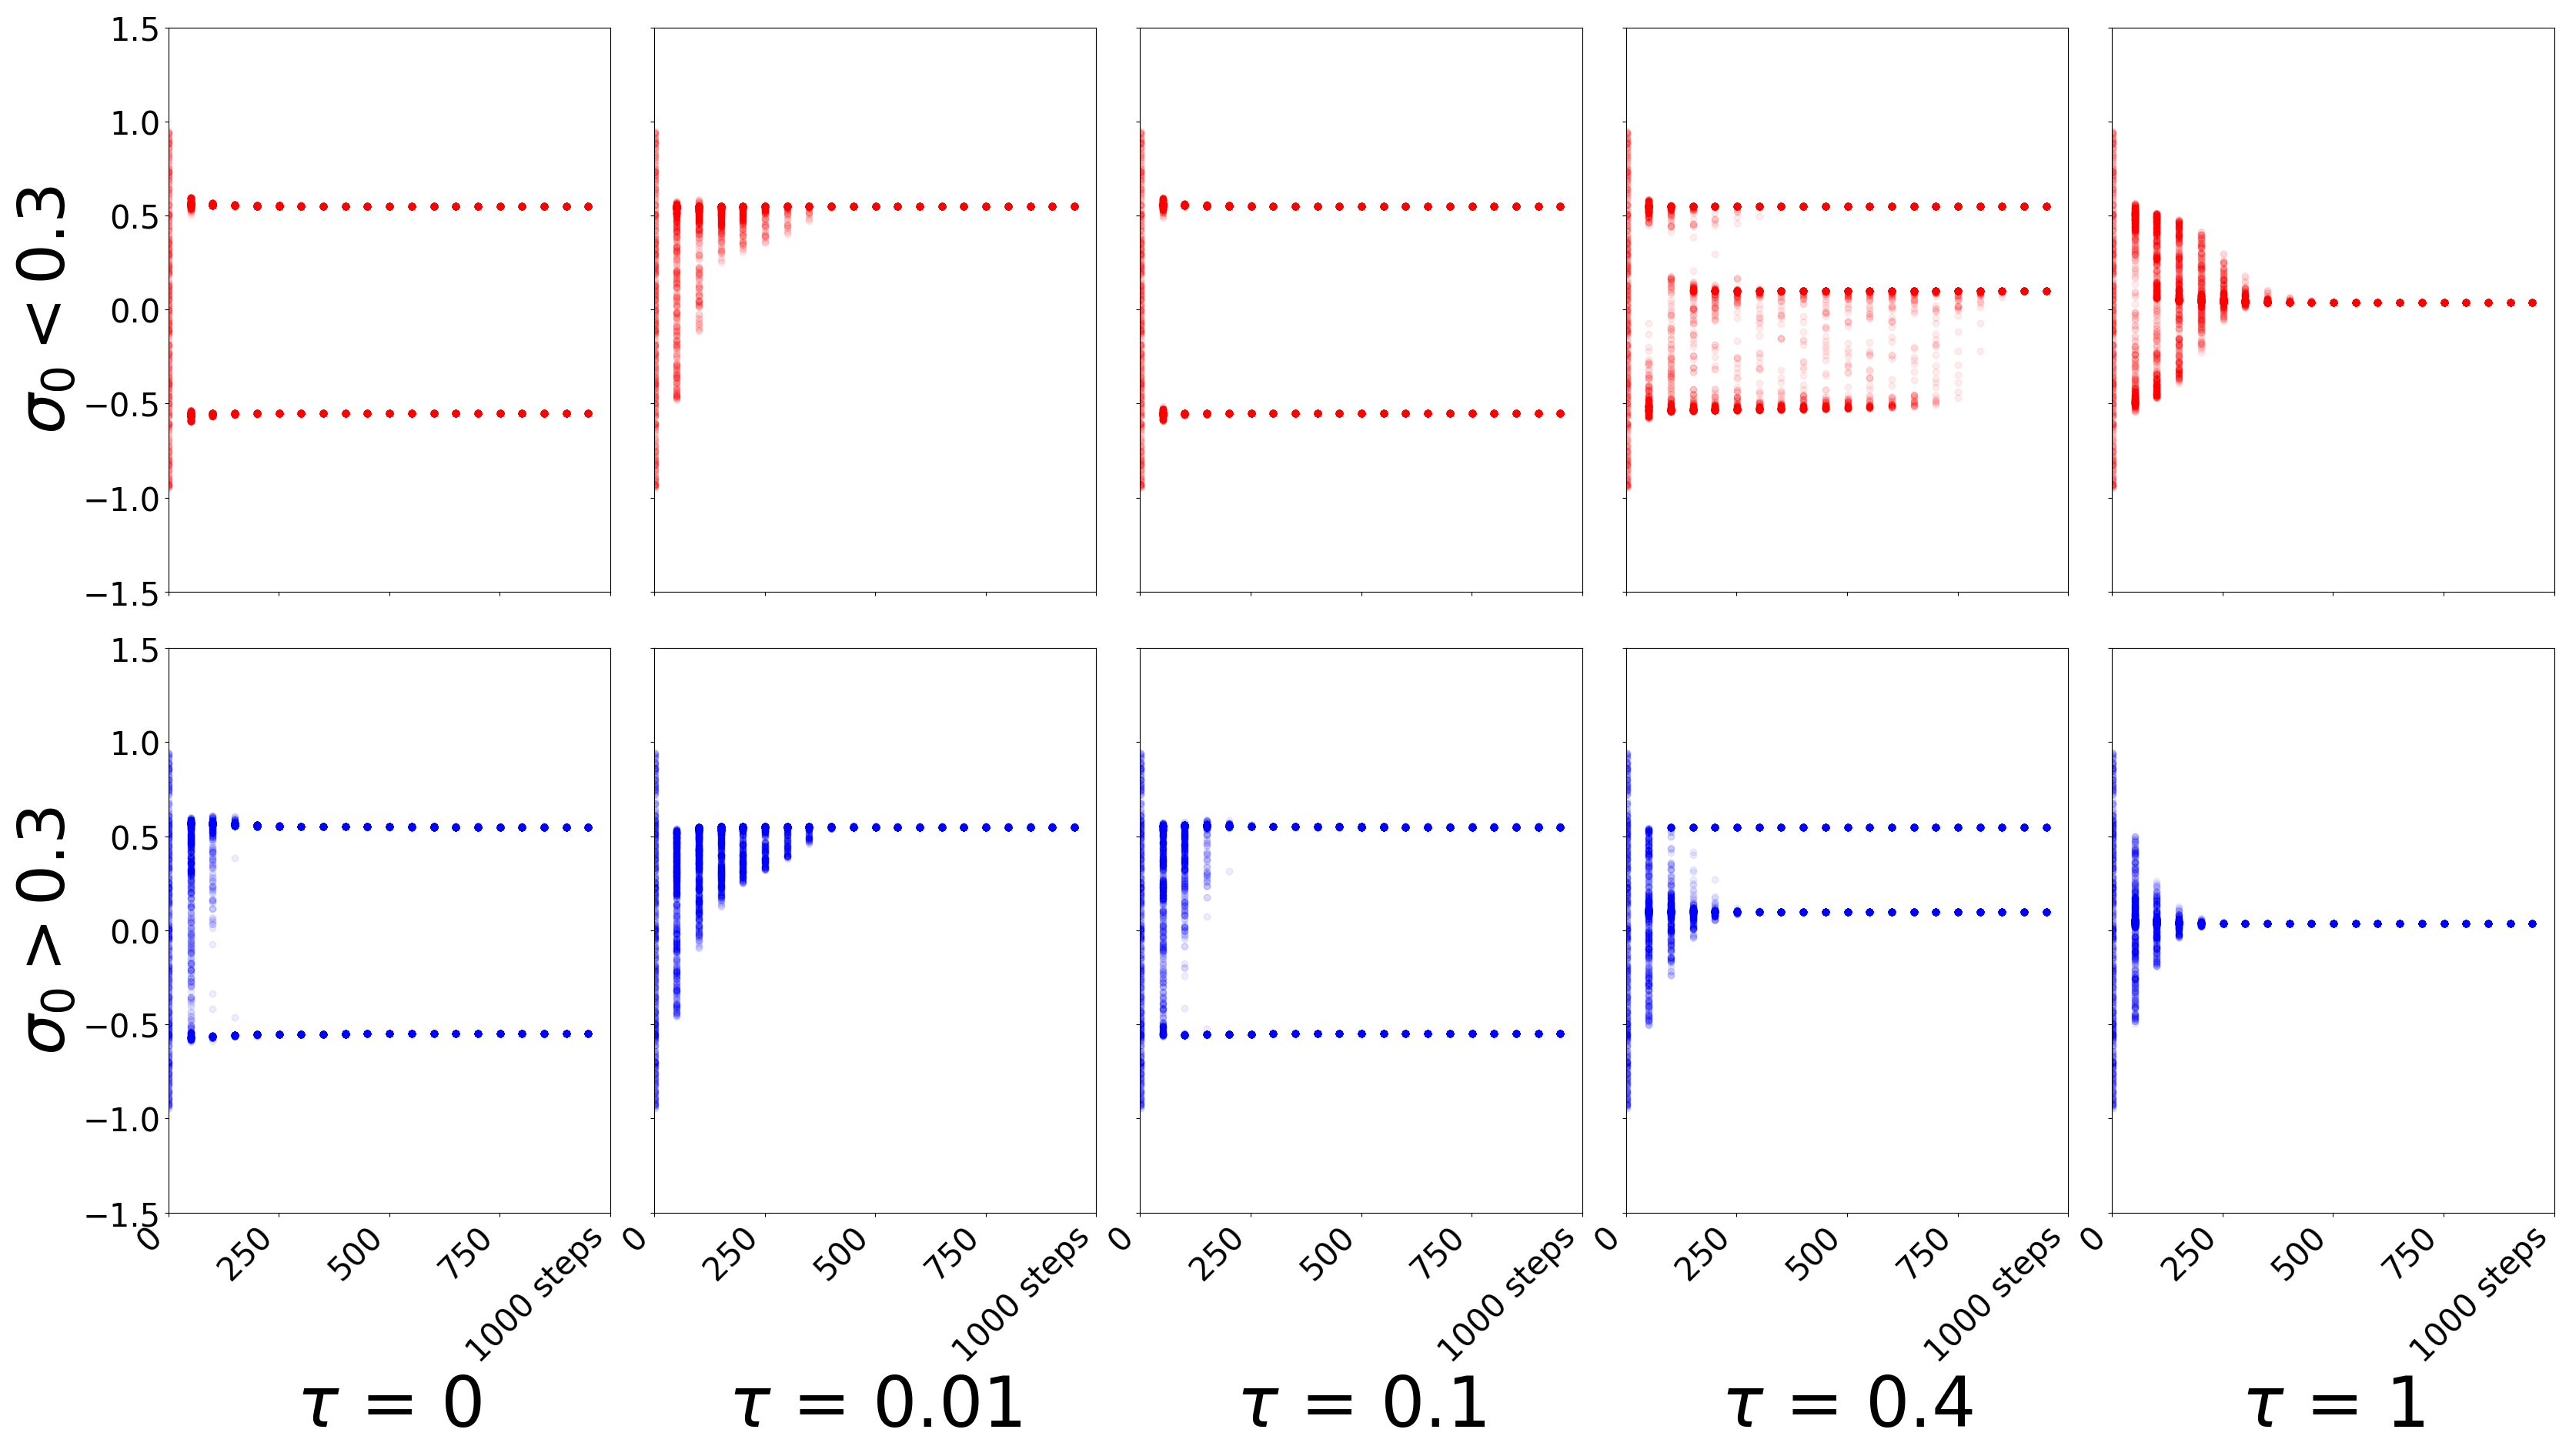
\includegraphics[width=1\columnwidth]{figs/bandit/notlearnQ/modes=1/adam/mean_reverse_optim=adam_modes=1_lr=0.01.png}
    \caption{Reverse KL, Adam. }
    \label{fig:bandit-mean-reverse-adam}
  \end{subfigure}
  
  \begin{subfigure}[b]{0.4\linewidth}
    \centering
    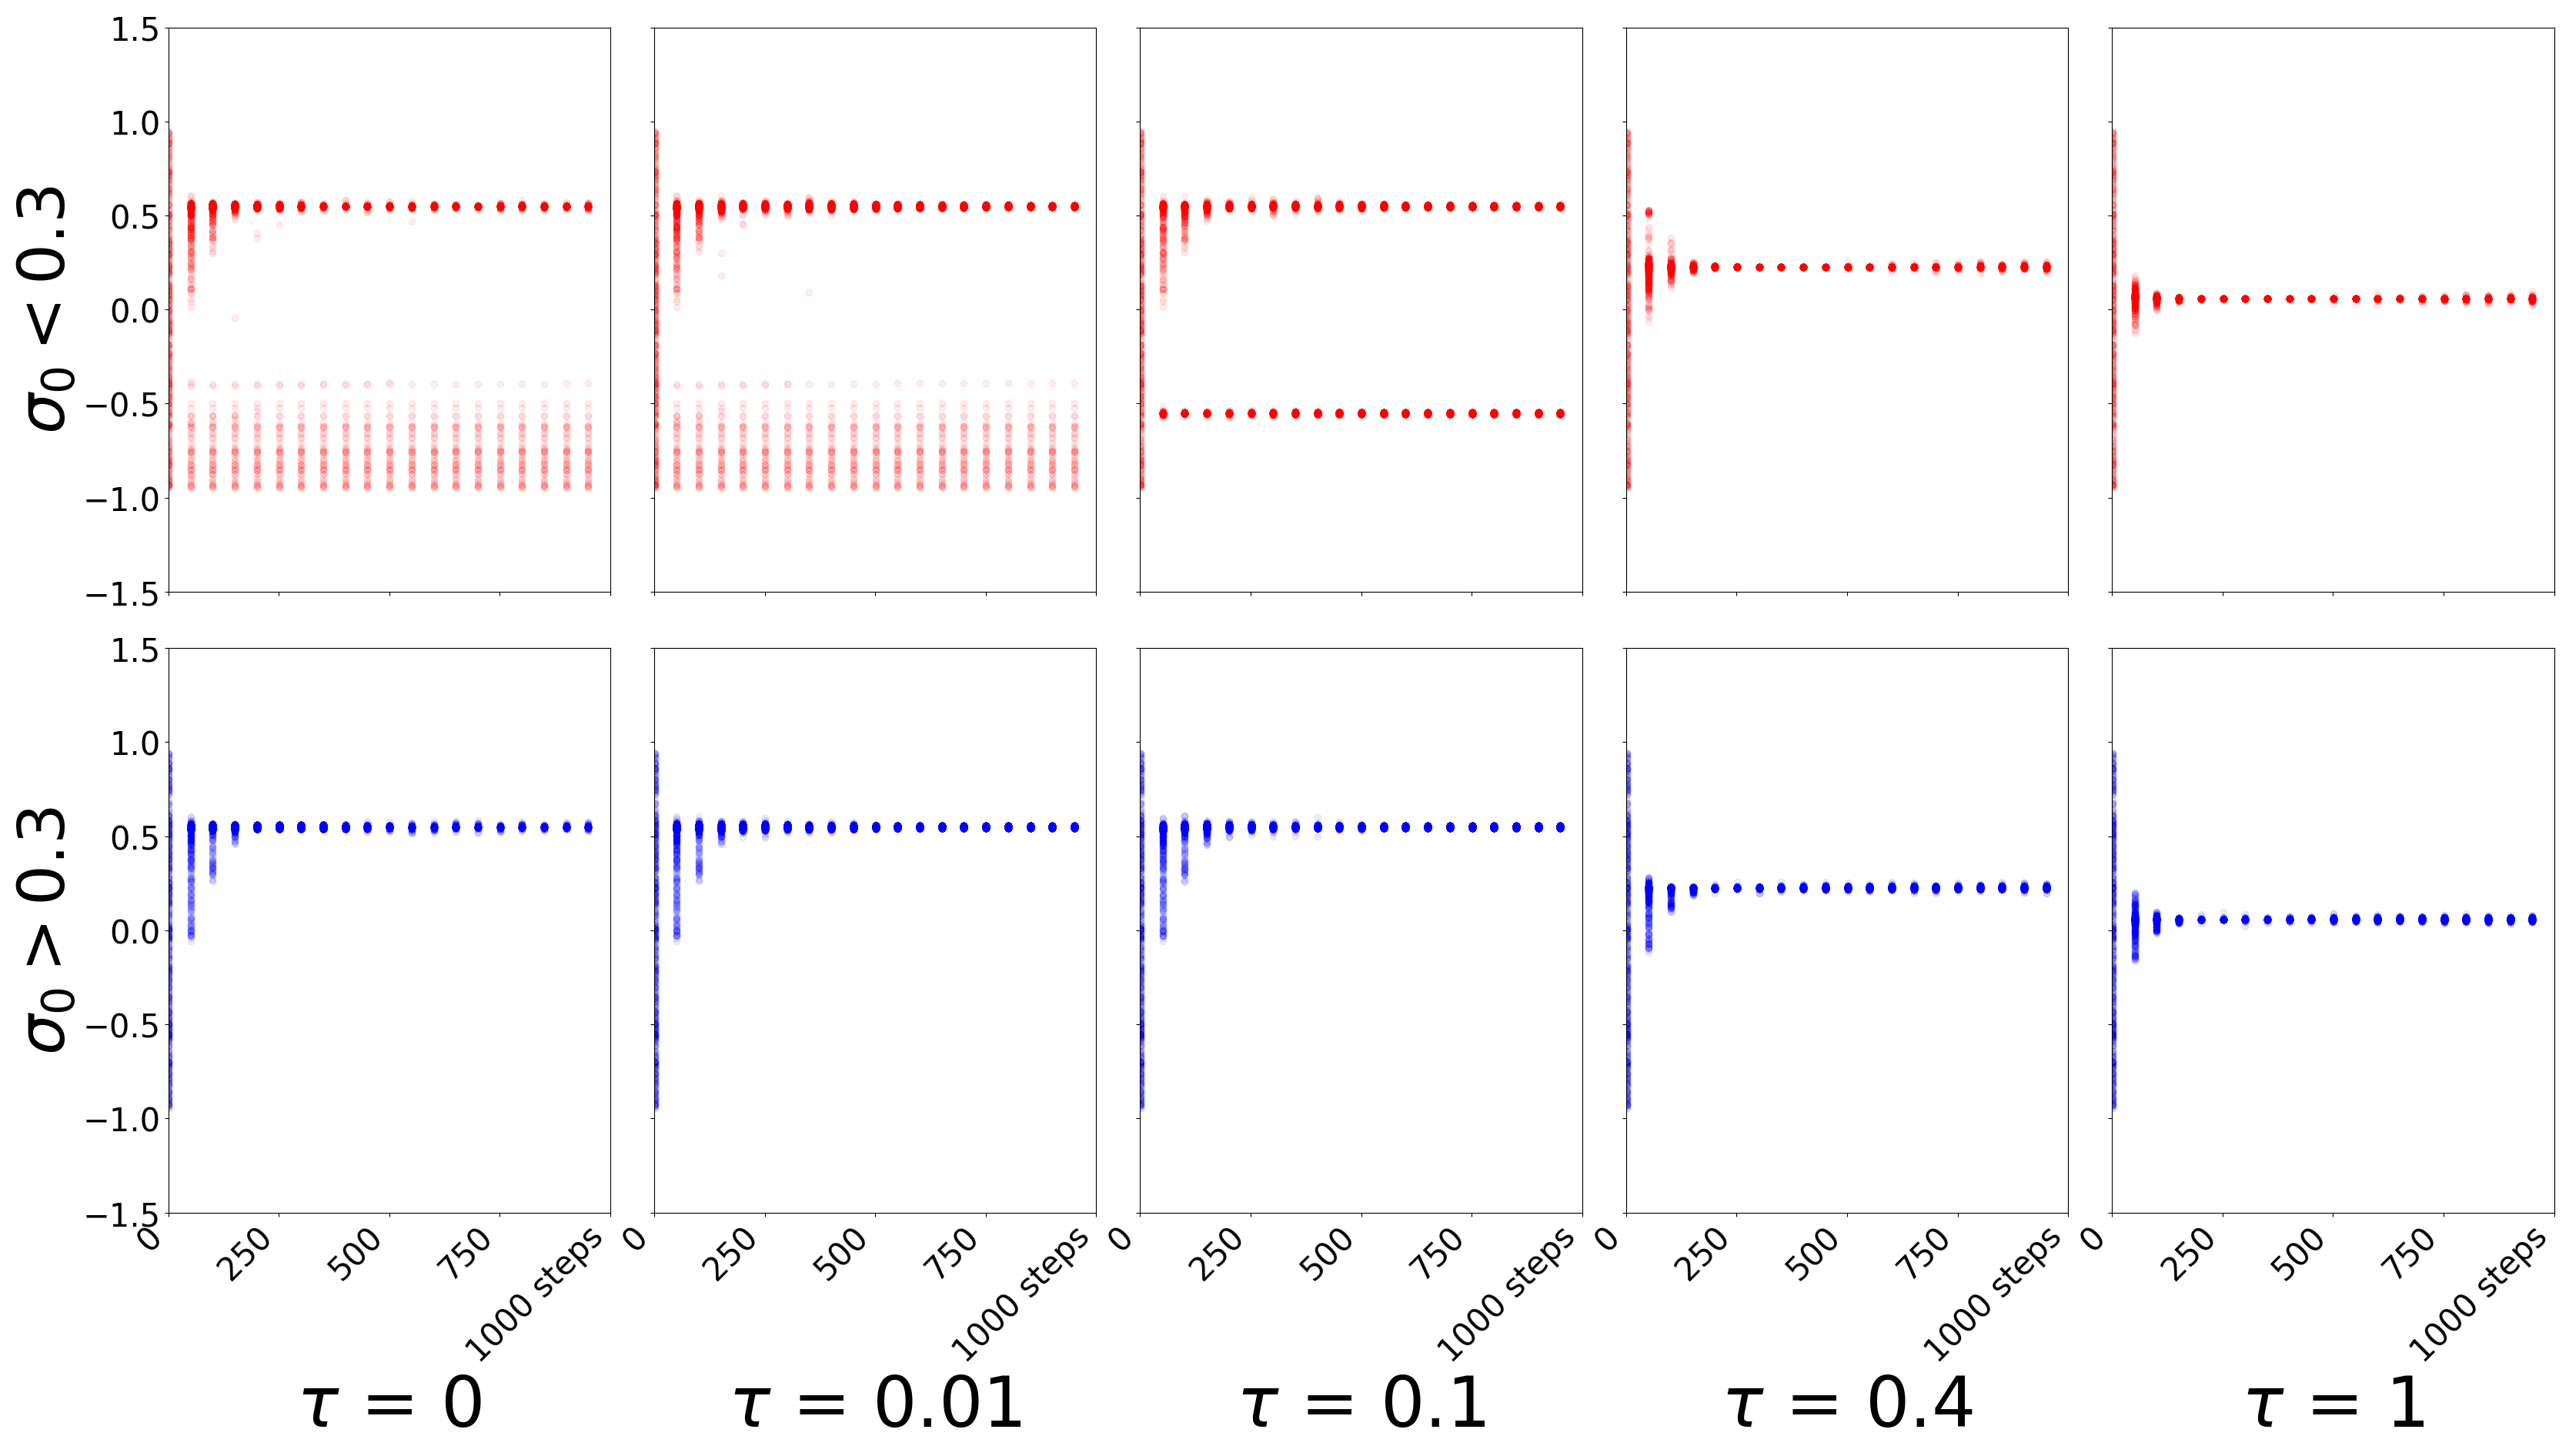
\includegraphics[width=1\columnwidth]{figs/bandit/notlearnQ/modes=1/rmsprop/mean_forward_optim=rmsprop_modes=1_lr=0.01.png}
    \caption{Forward KL, RMSprop.}
    \label{fig:bandit-mean-forward-rmsprop}
  \end{subfigure}%
  \begin{subfigure}[b]{0.4\linewidth}
    \centering
    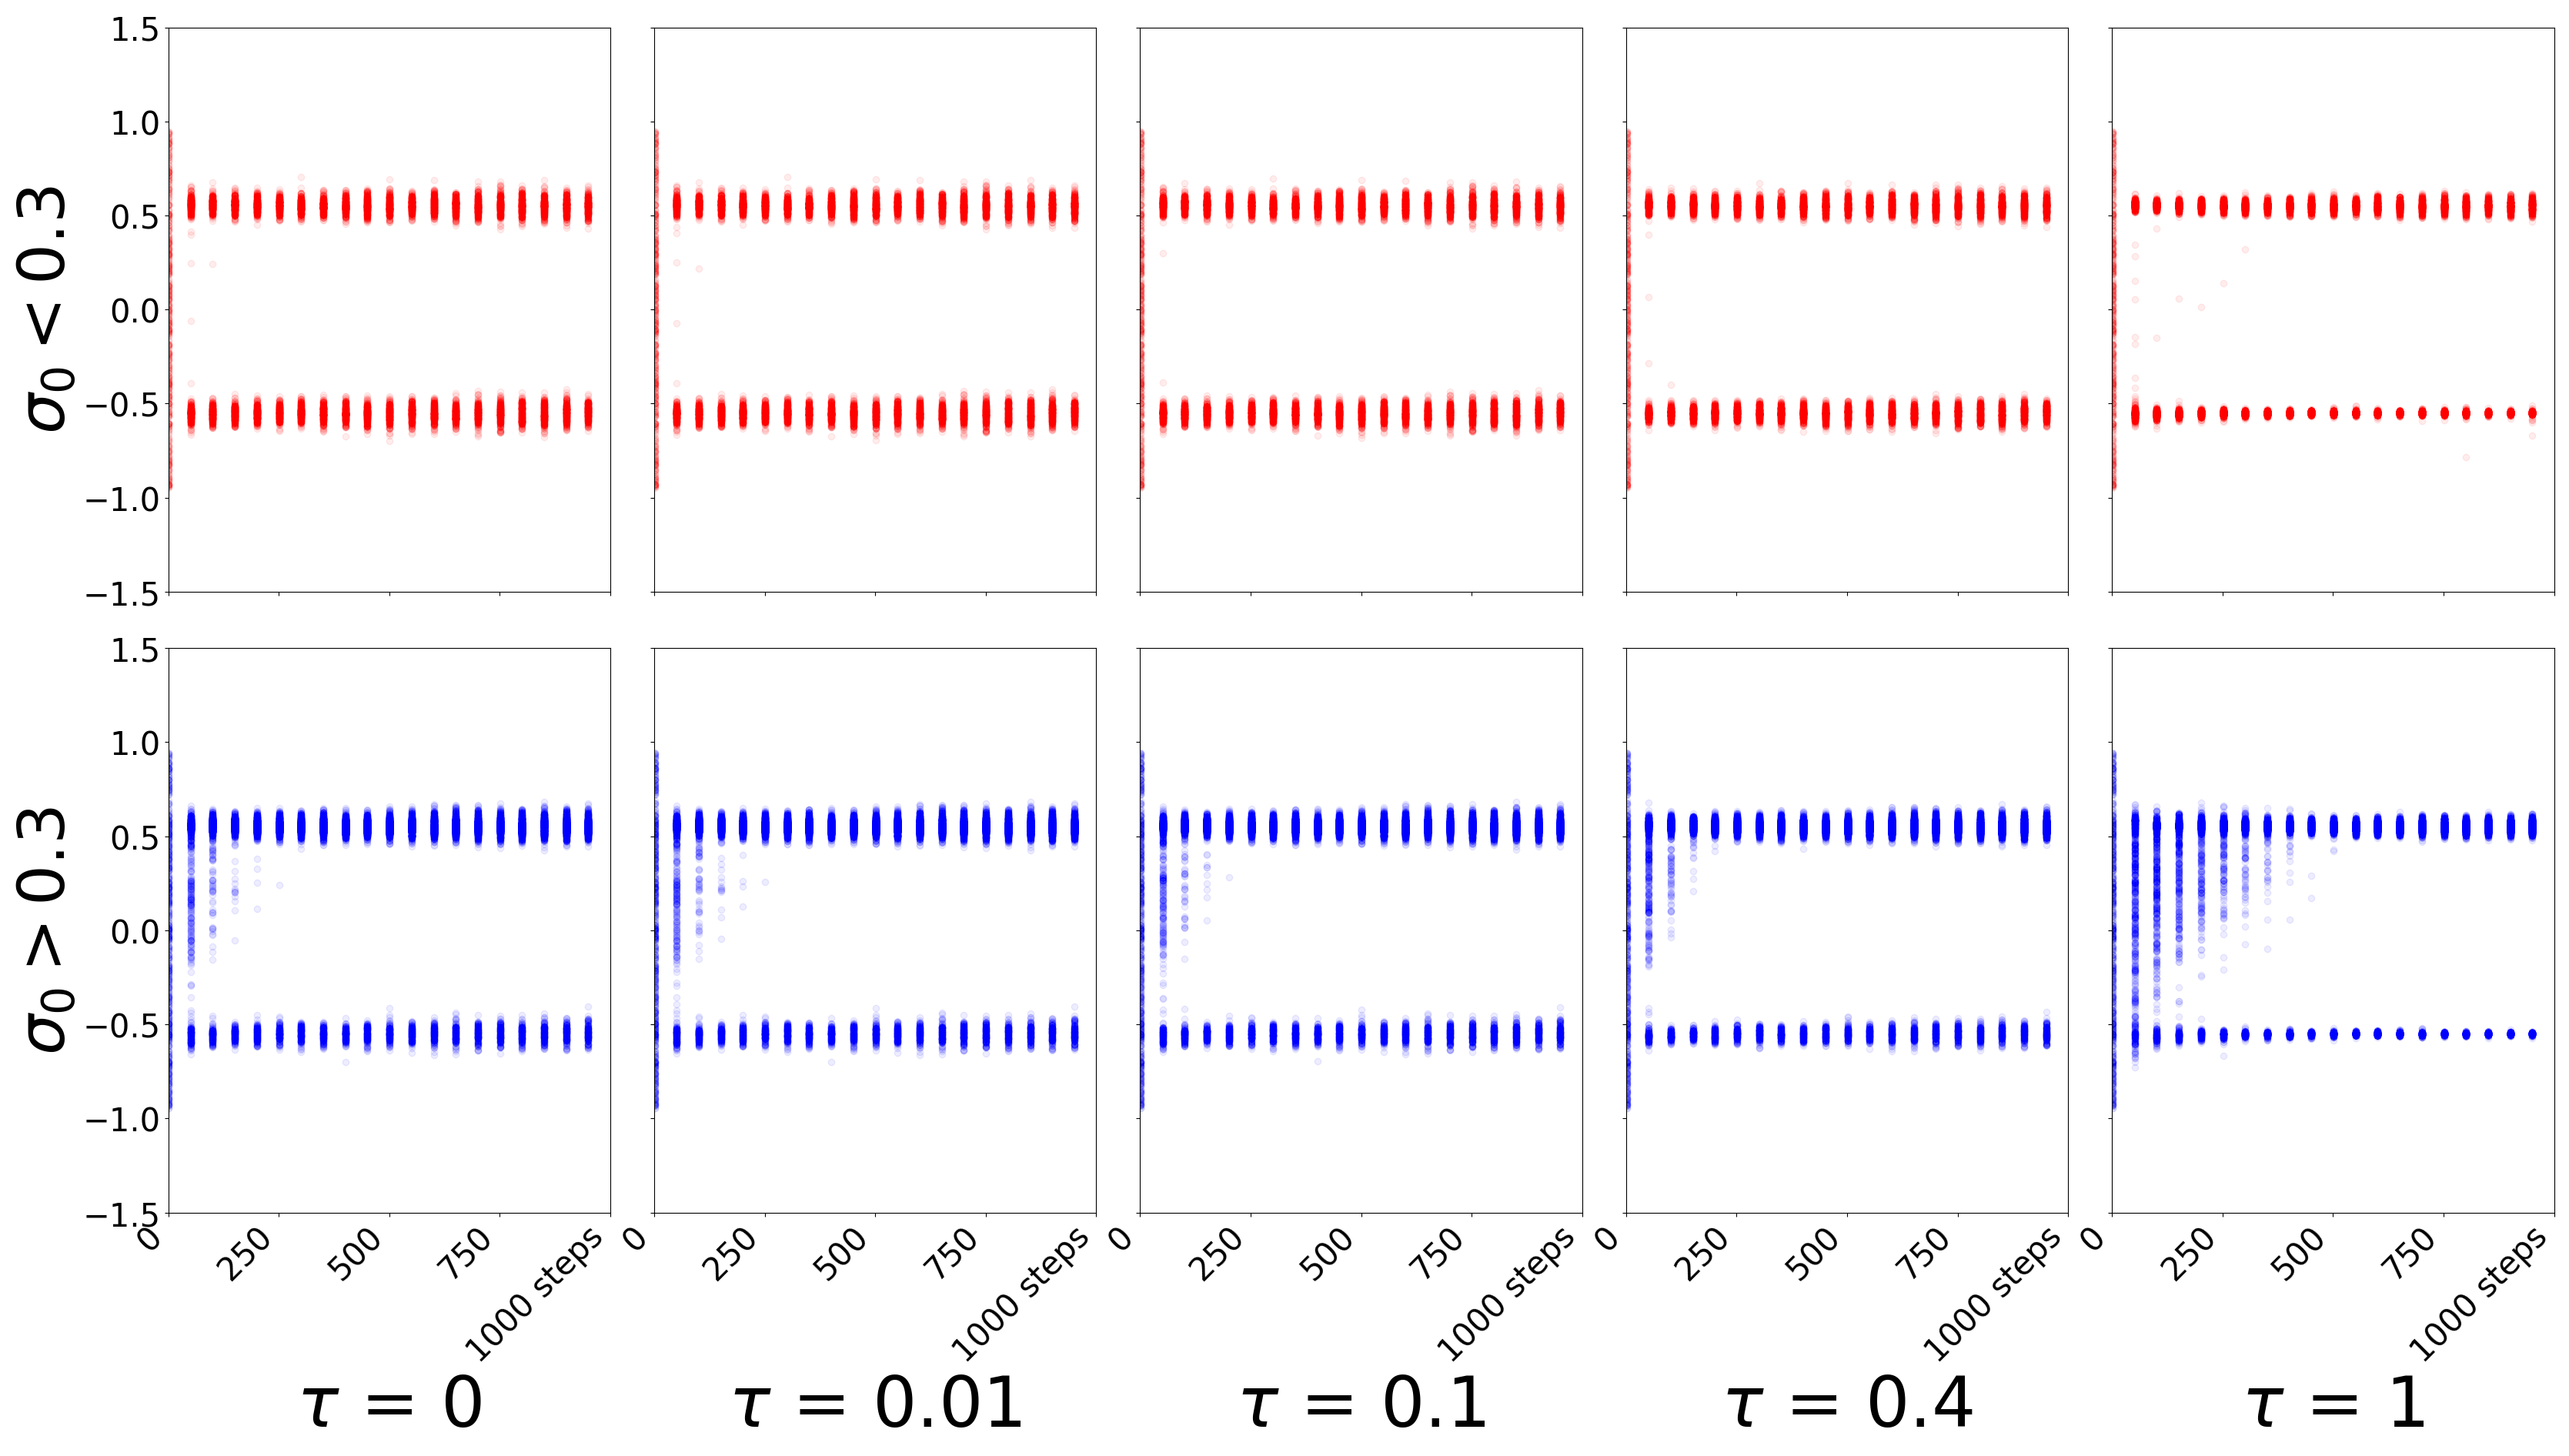
\includegraphics[width=1\columnwidth]{figs/bandit/notlearnQ/modes=1/rmsprop/mean_reverse_optim=rmsprop_modes=1_lr=0.01.png}
    \caption{Reverse KL, RMSprop.}
    \label{fig:bandit-mean-reverse-rmsprop}
  \end{subfigure}
  
  \begin{subfigure}[b]{0.4\linewidth}
    \centering
    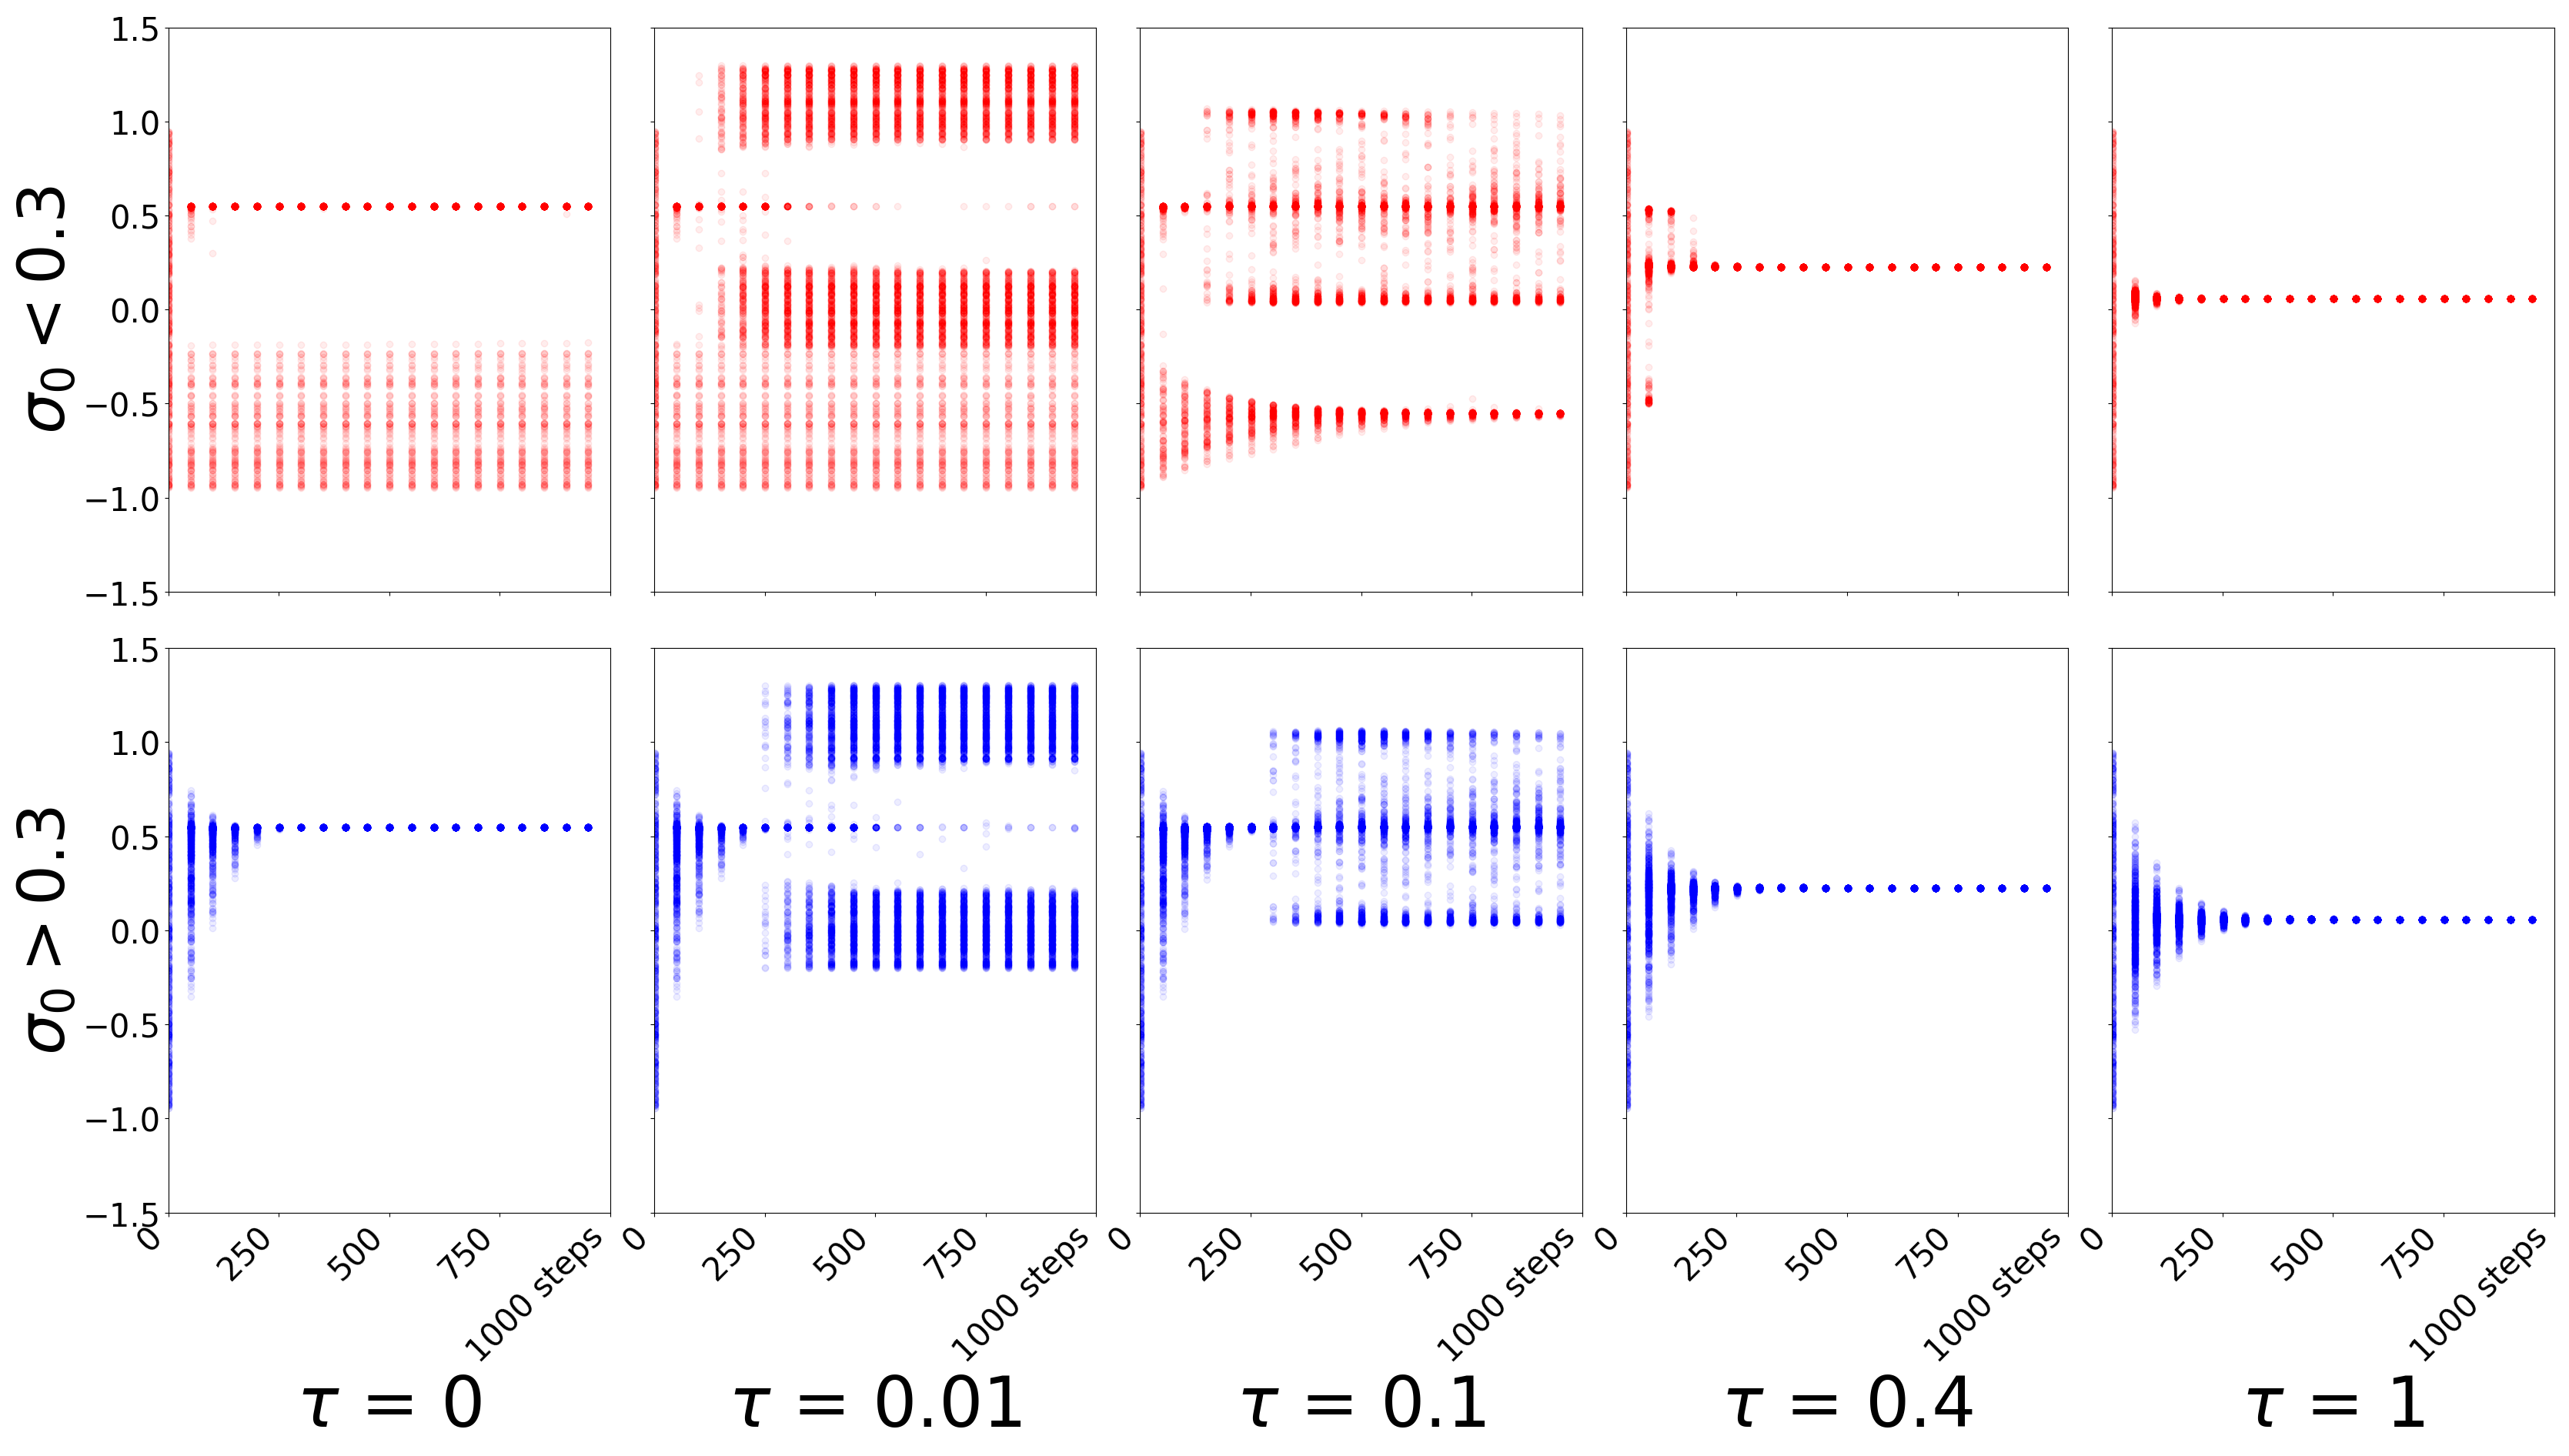
\includegraphics[width=1\columnwidth]{figs/bandit/notlearnQ/modes=1/sgd/mean_forward_optim=sgd_modes=1_lr=0.01.png}
    \caption{Forward KL, SGD.}
    \label{fig:bandit-mean-forward-sgd}
  \end{subfigure}%
  \begin{subfigure}[b]{0.4\linewidth}
    \centering
    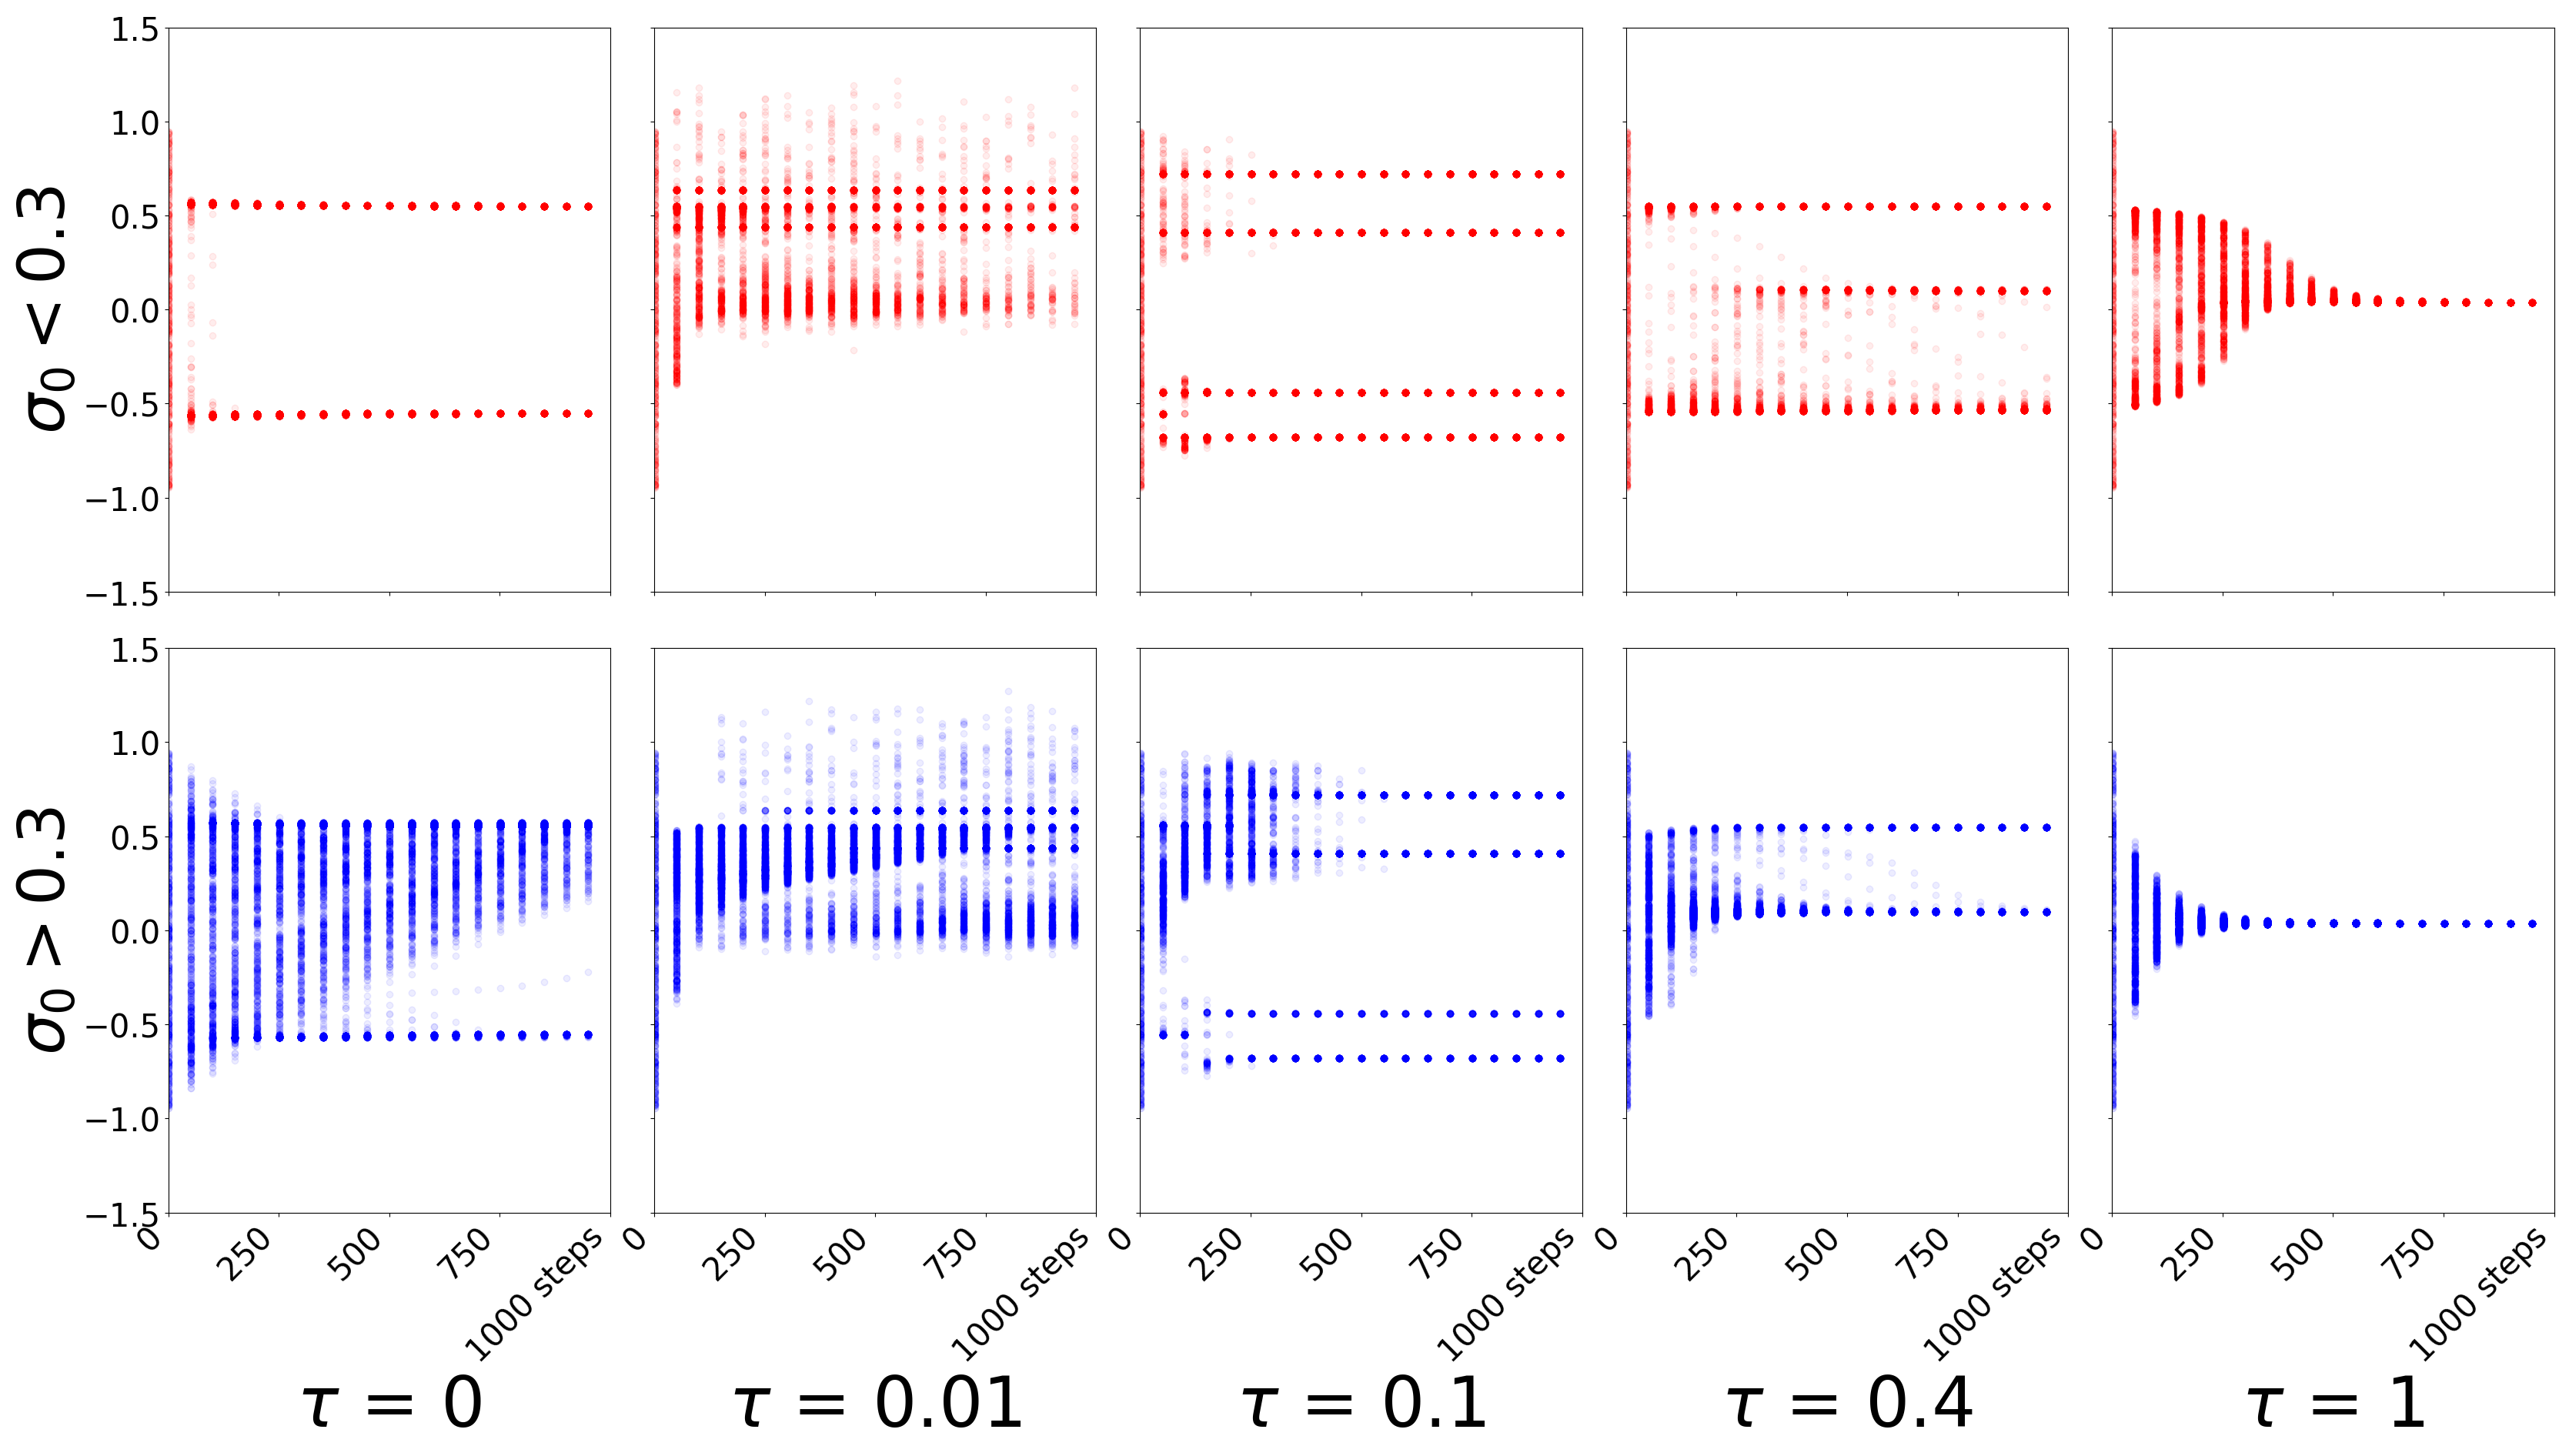
\includegraphics[width=1\columnwidth]{figs/bandit/notlearnQ/modes=1/sgd/mean_reverse_optim=sgd_modes=1_lr=0.01.png}
    \caption{Reverse KL, SGD.}
    \label{fig:bandit-mean-reverse-sgd}
  \end{subfigure}
  \caption{Mean over time with unimodal policy. }
\end{figure}

\begin{figure}[!ht]
  \centering
  \begin{subfigure}[b]{0.4\linewidth}
    \centering
    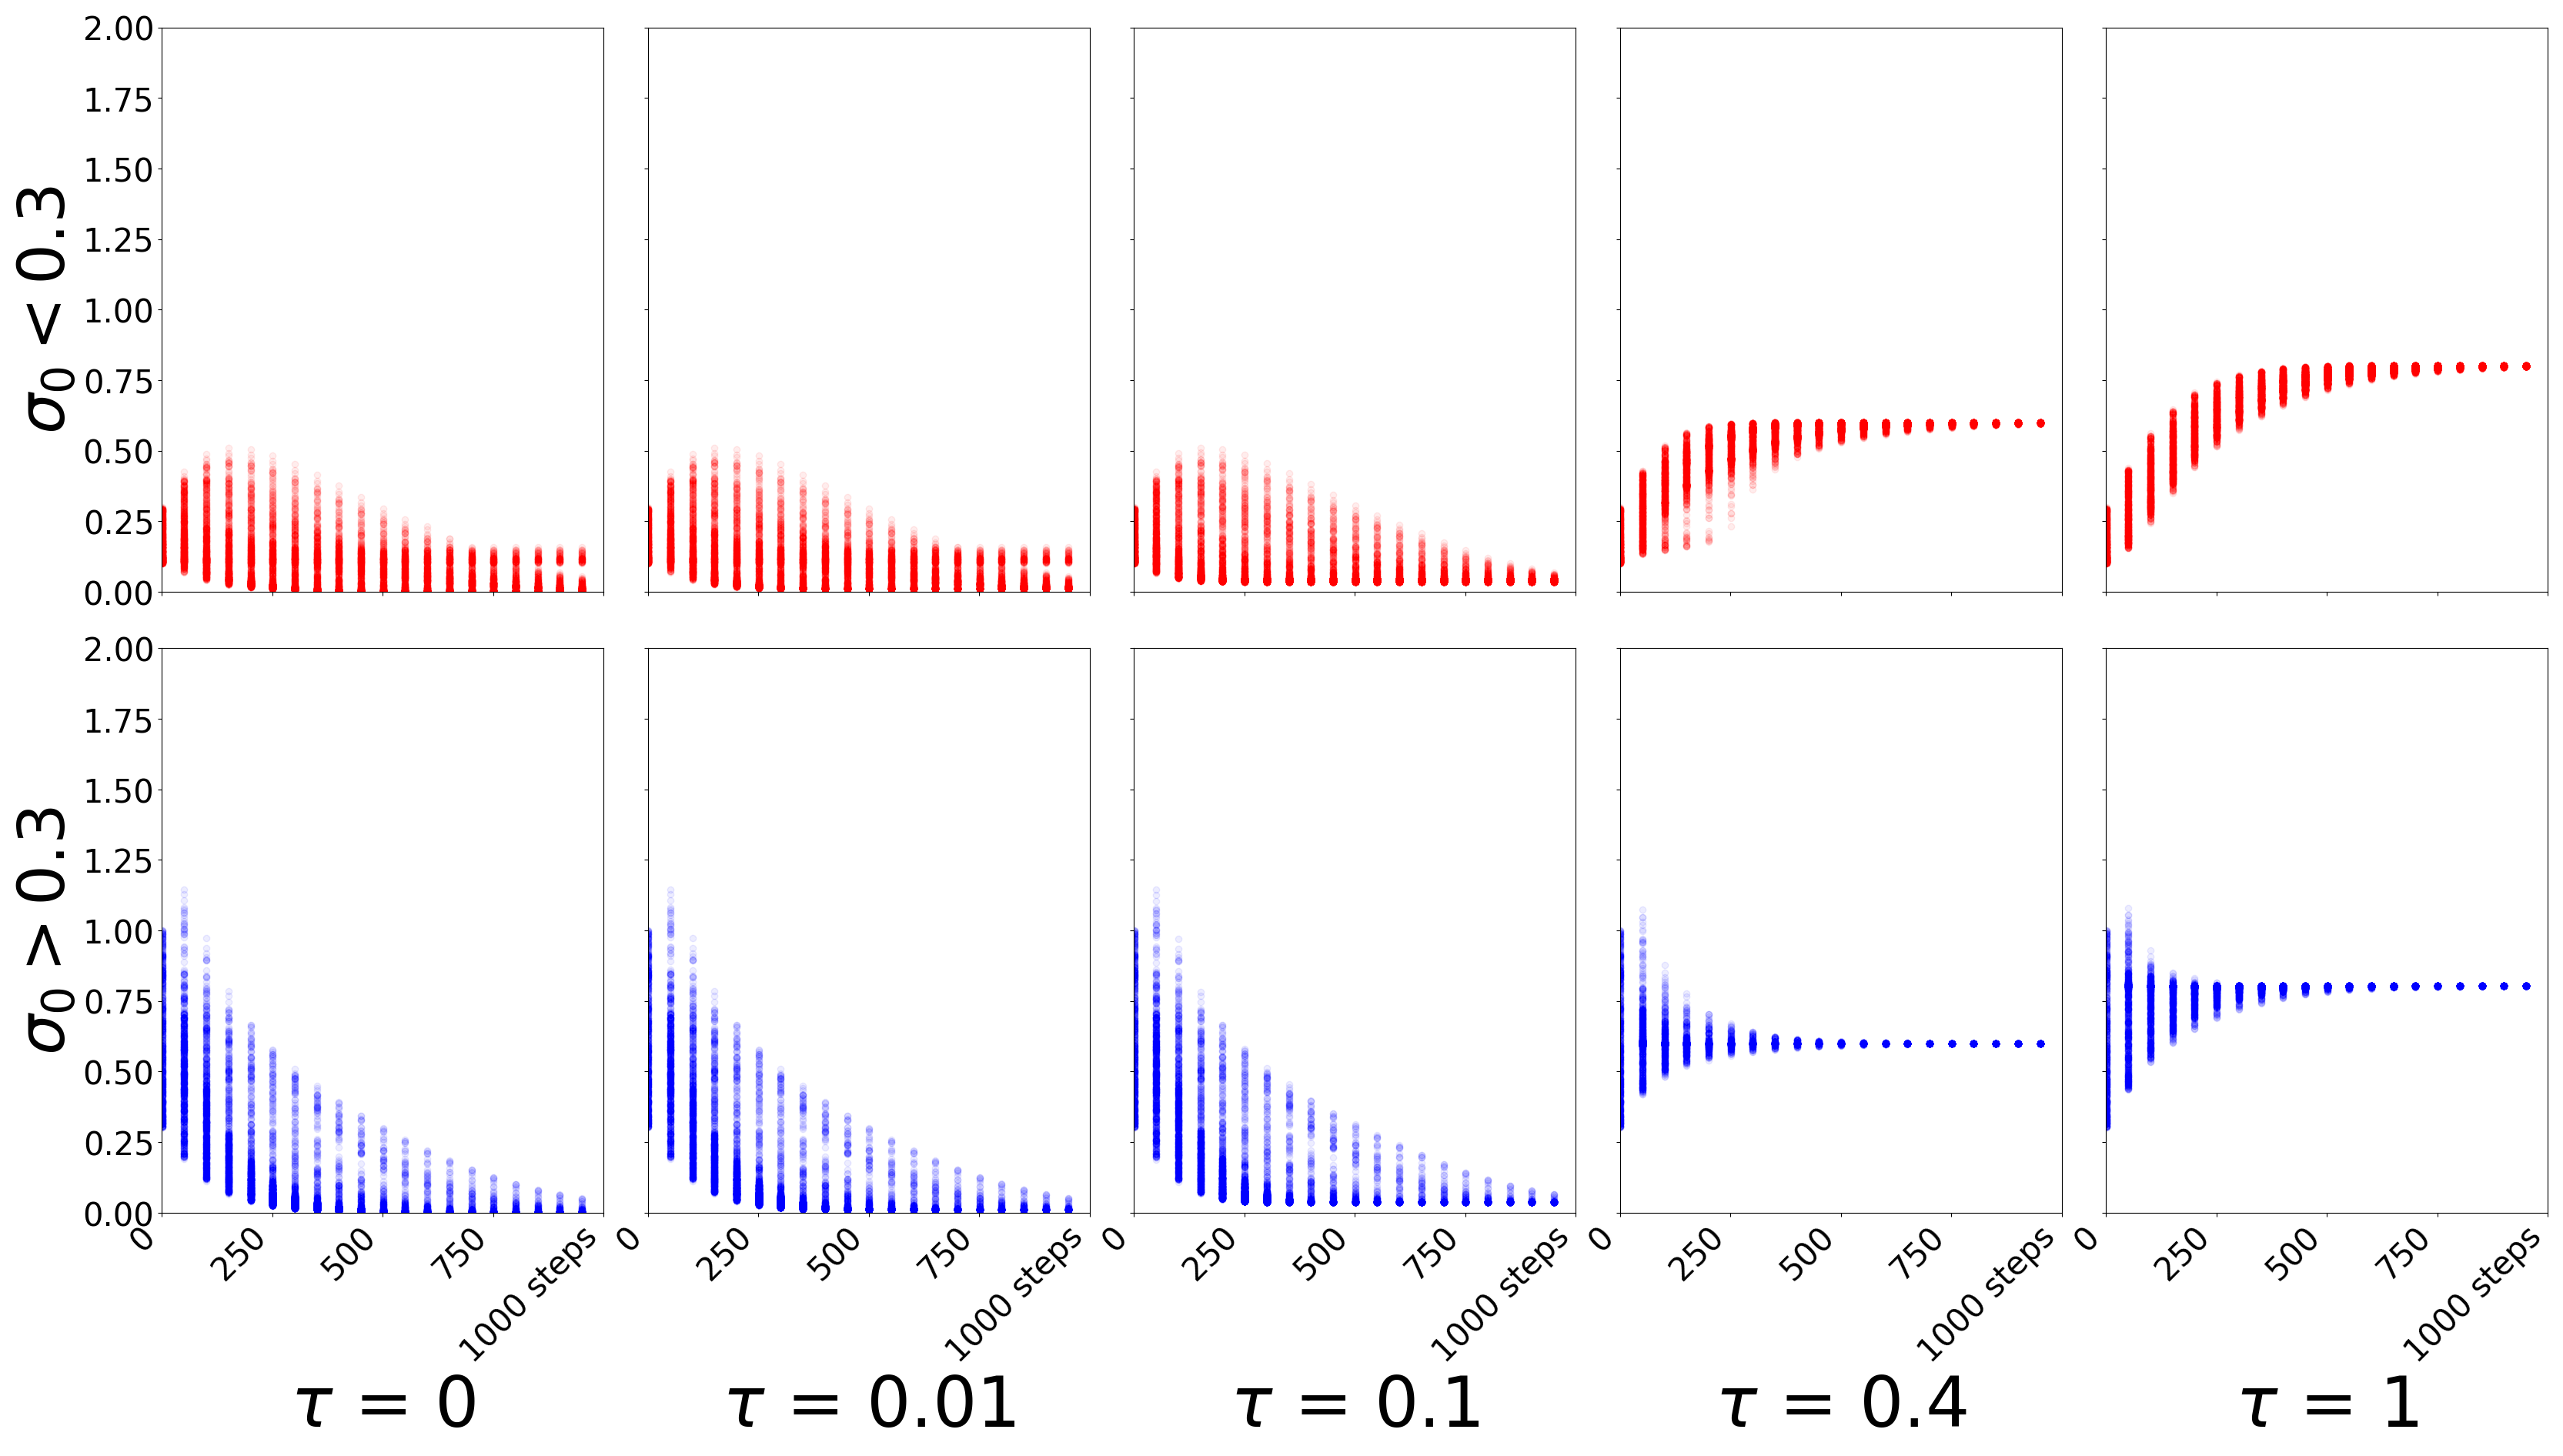
\includegraphics[width=1\columnwidth]{figs/bandit/notlearnQ/modes=1/adam/std_forward_optim=adam_modes=1_lr=0.01.png}
    \caption{Forward KL, Adam.}
    \label{fig:bandit-std-forward-adam}
  \end{subfigure}%
  \begin{subfigure}[b]{0.4\linewidth}
    \centering
    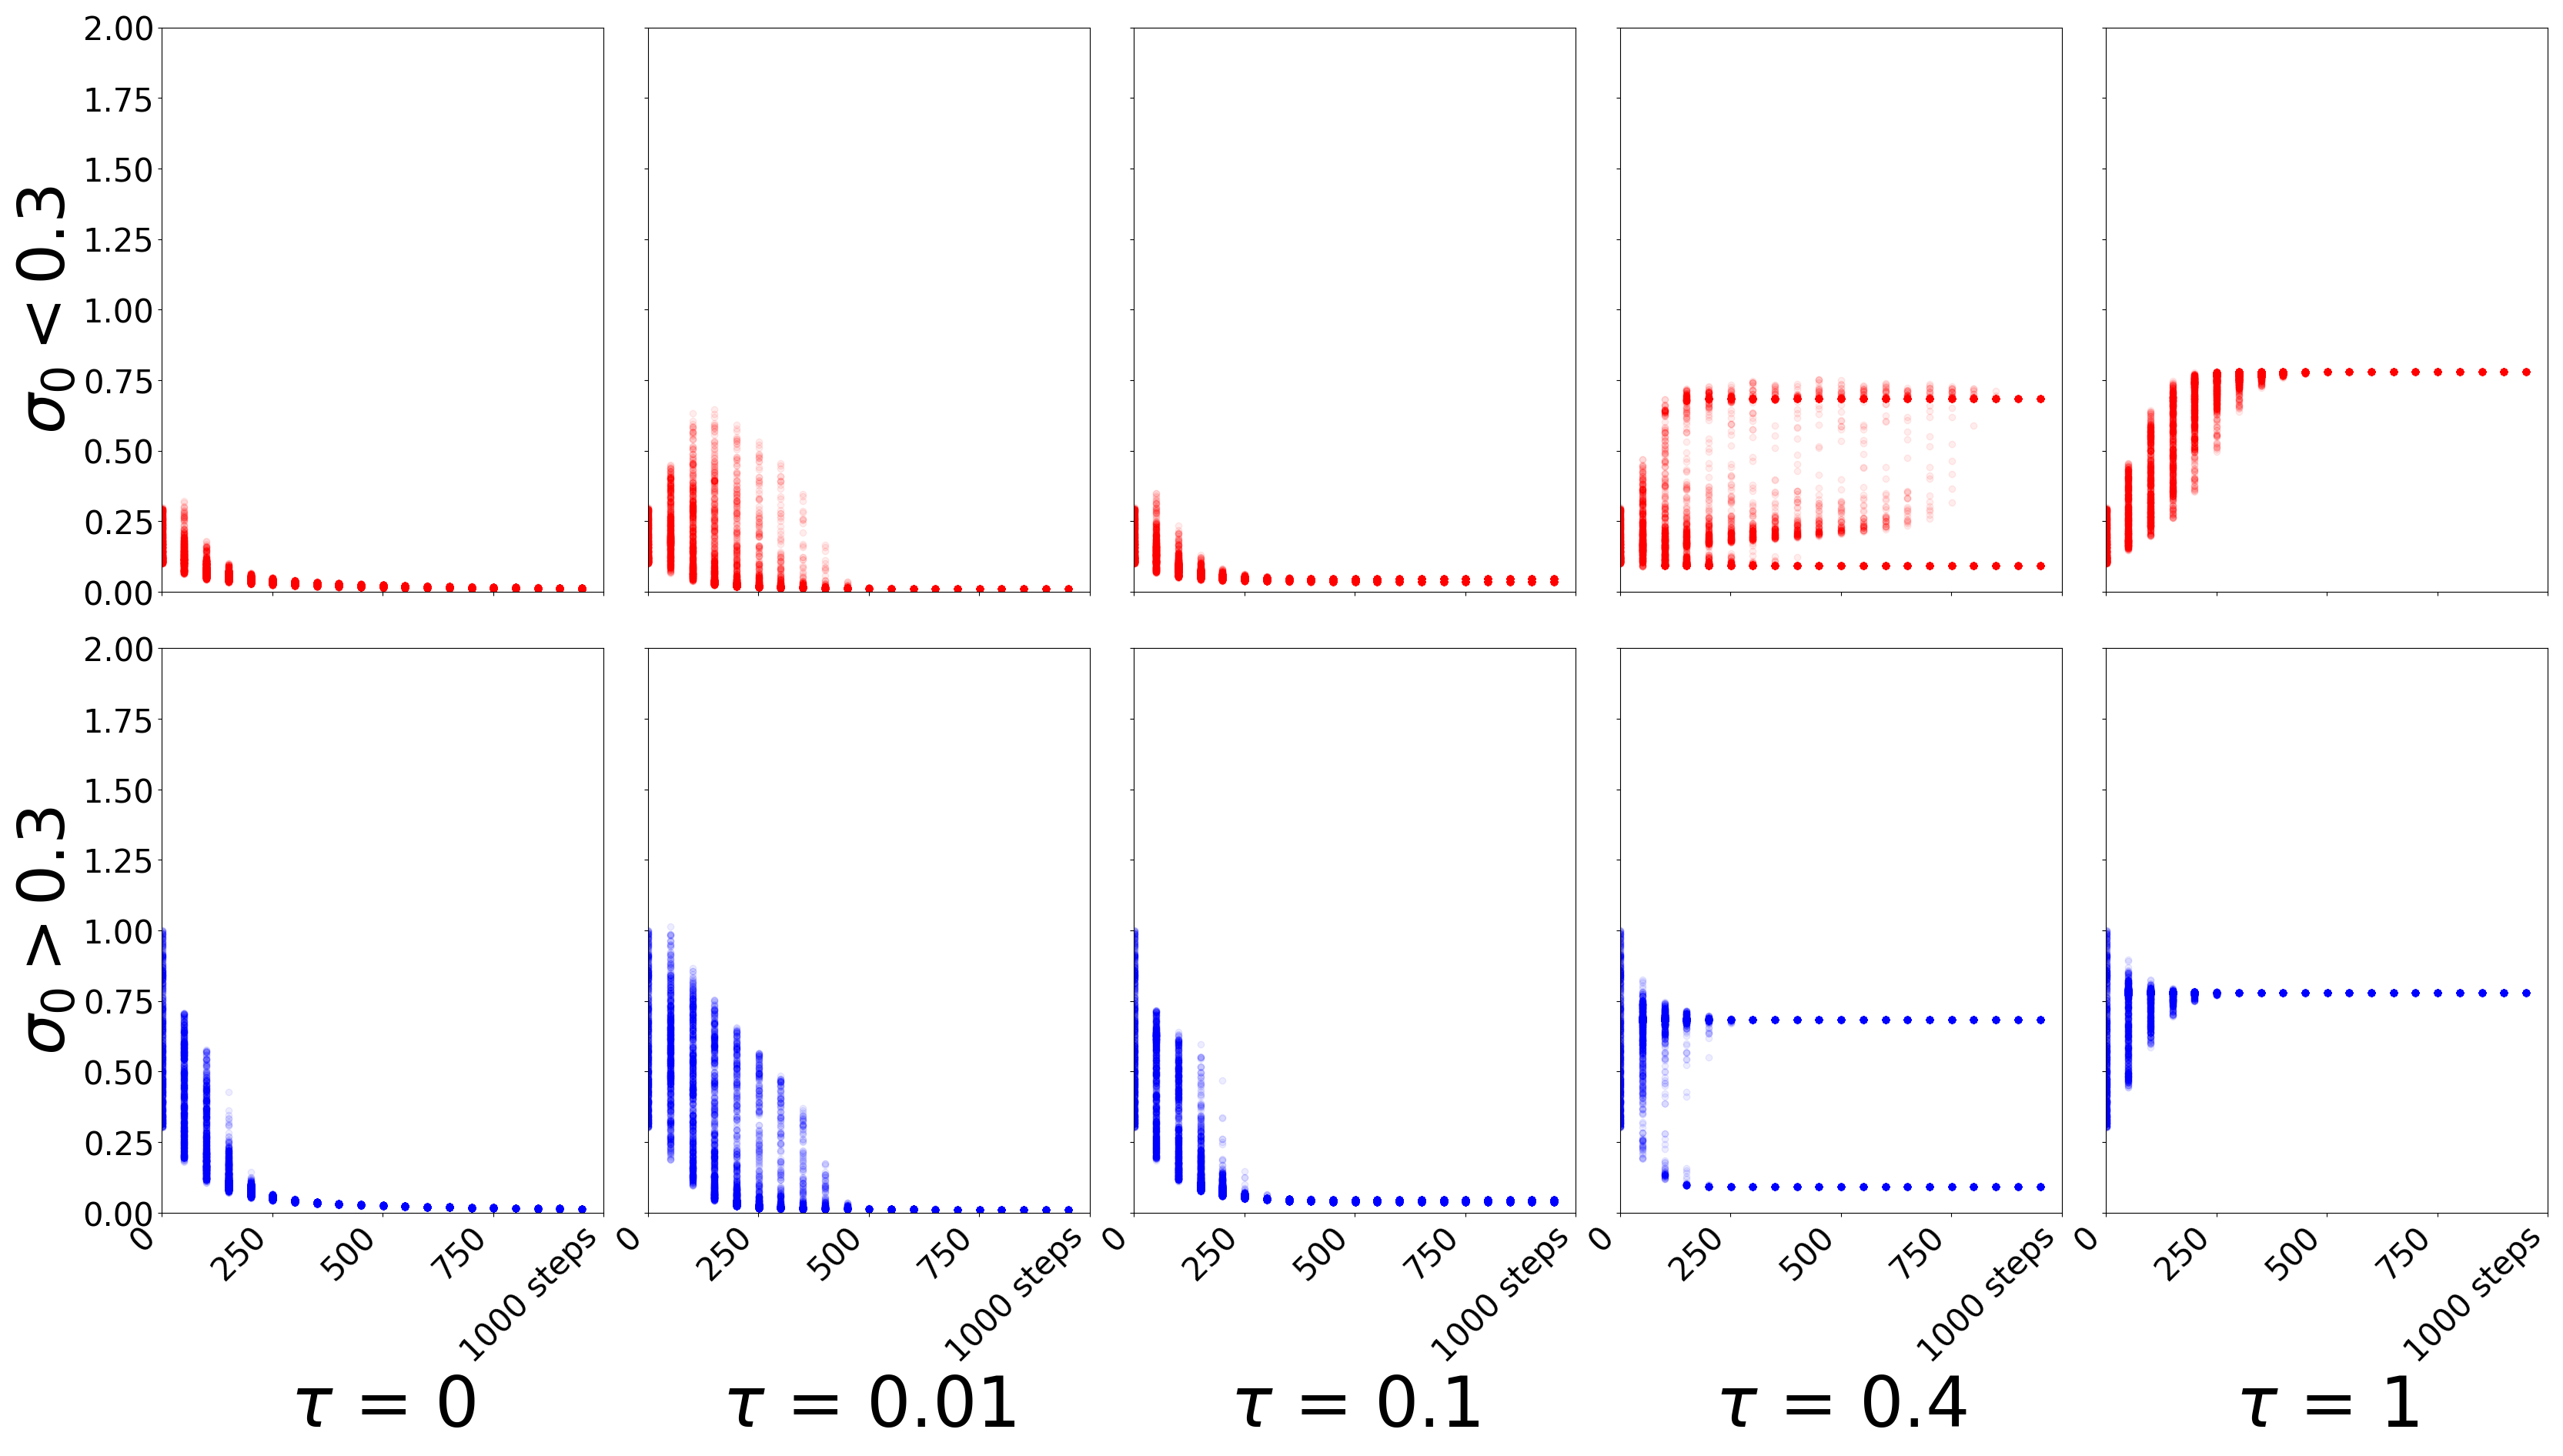
\includegraphics[width=1\columnwidth]{figs/bandit/notlearnQ/modes=1/adam/std_reverse_optim=adam_modes=1_lr=0.01.png}
    \caption{Reverse KL, Adam. }
    \label{fig:bandit-std-reverse-adam}
  \end{subfigure}
  
  \begin{subfigure}[b]{0.4\linewidth}
    \centering
    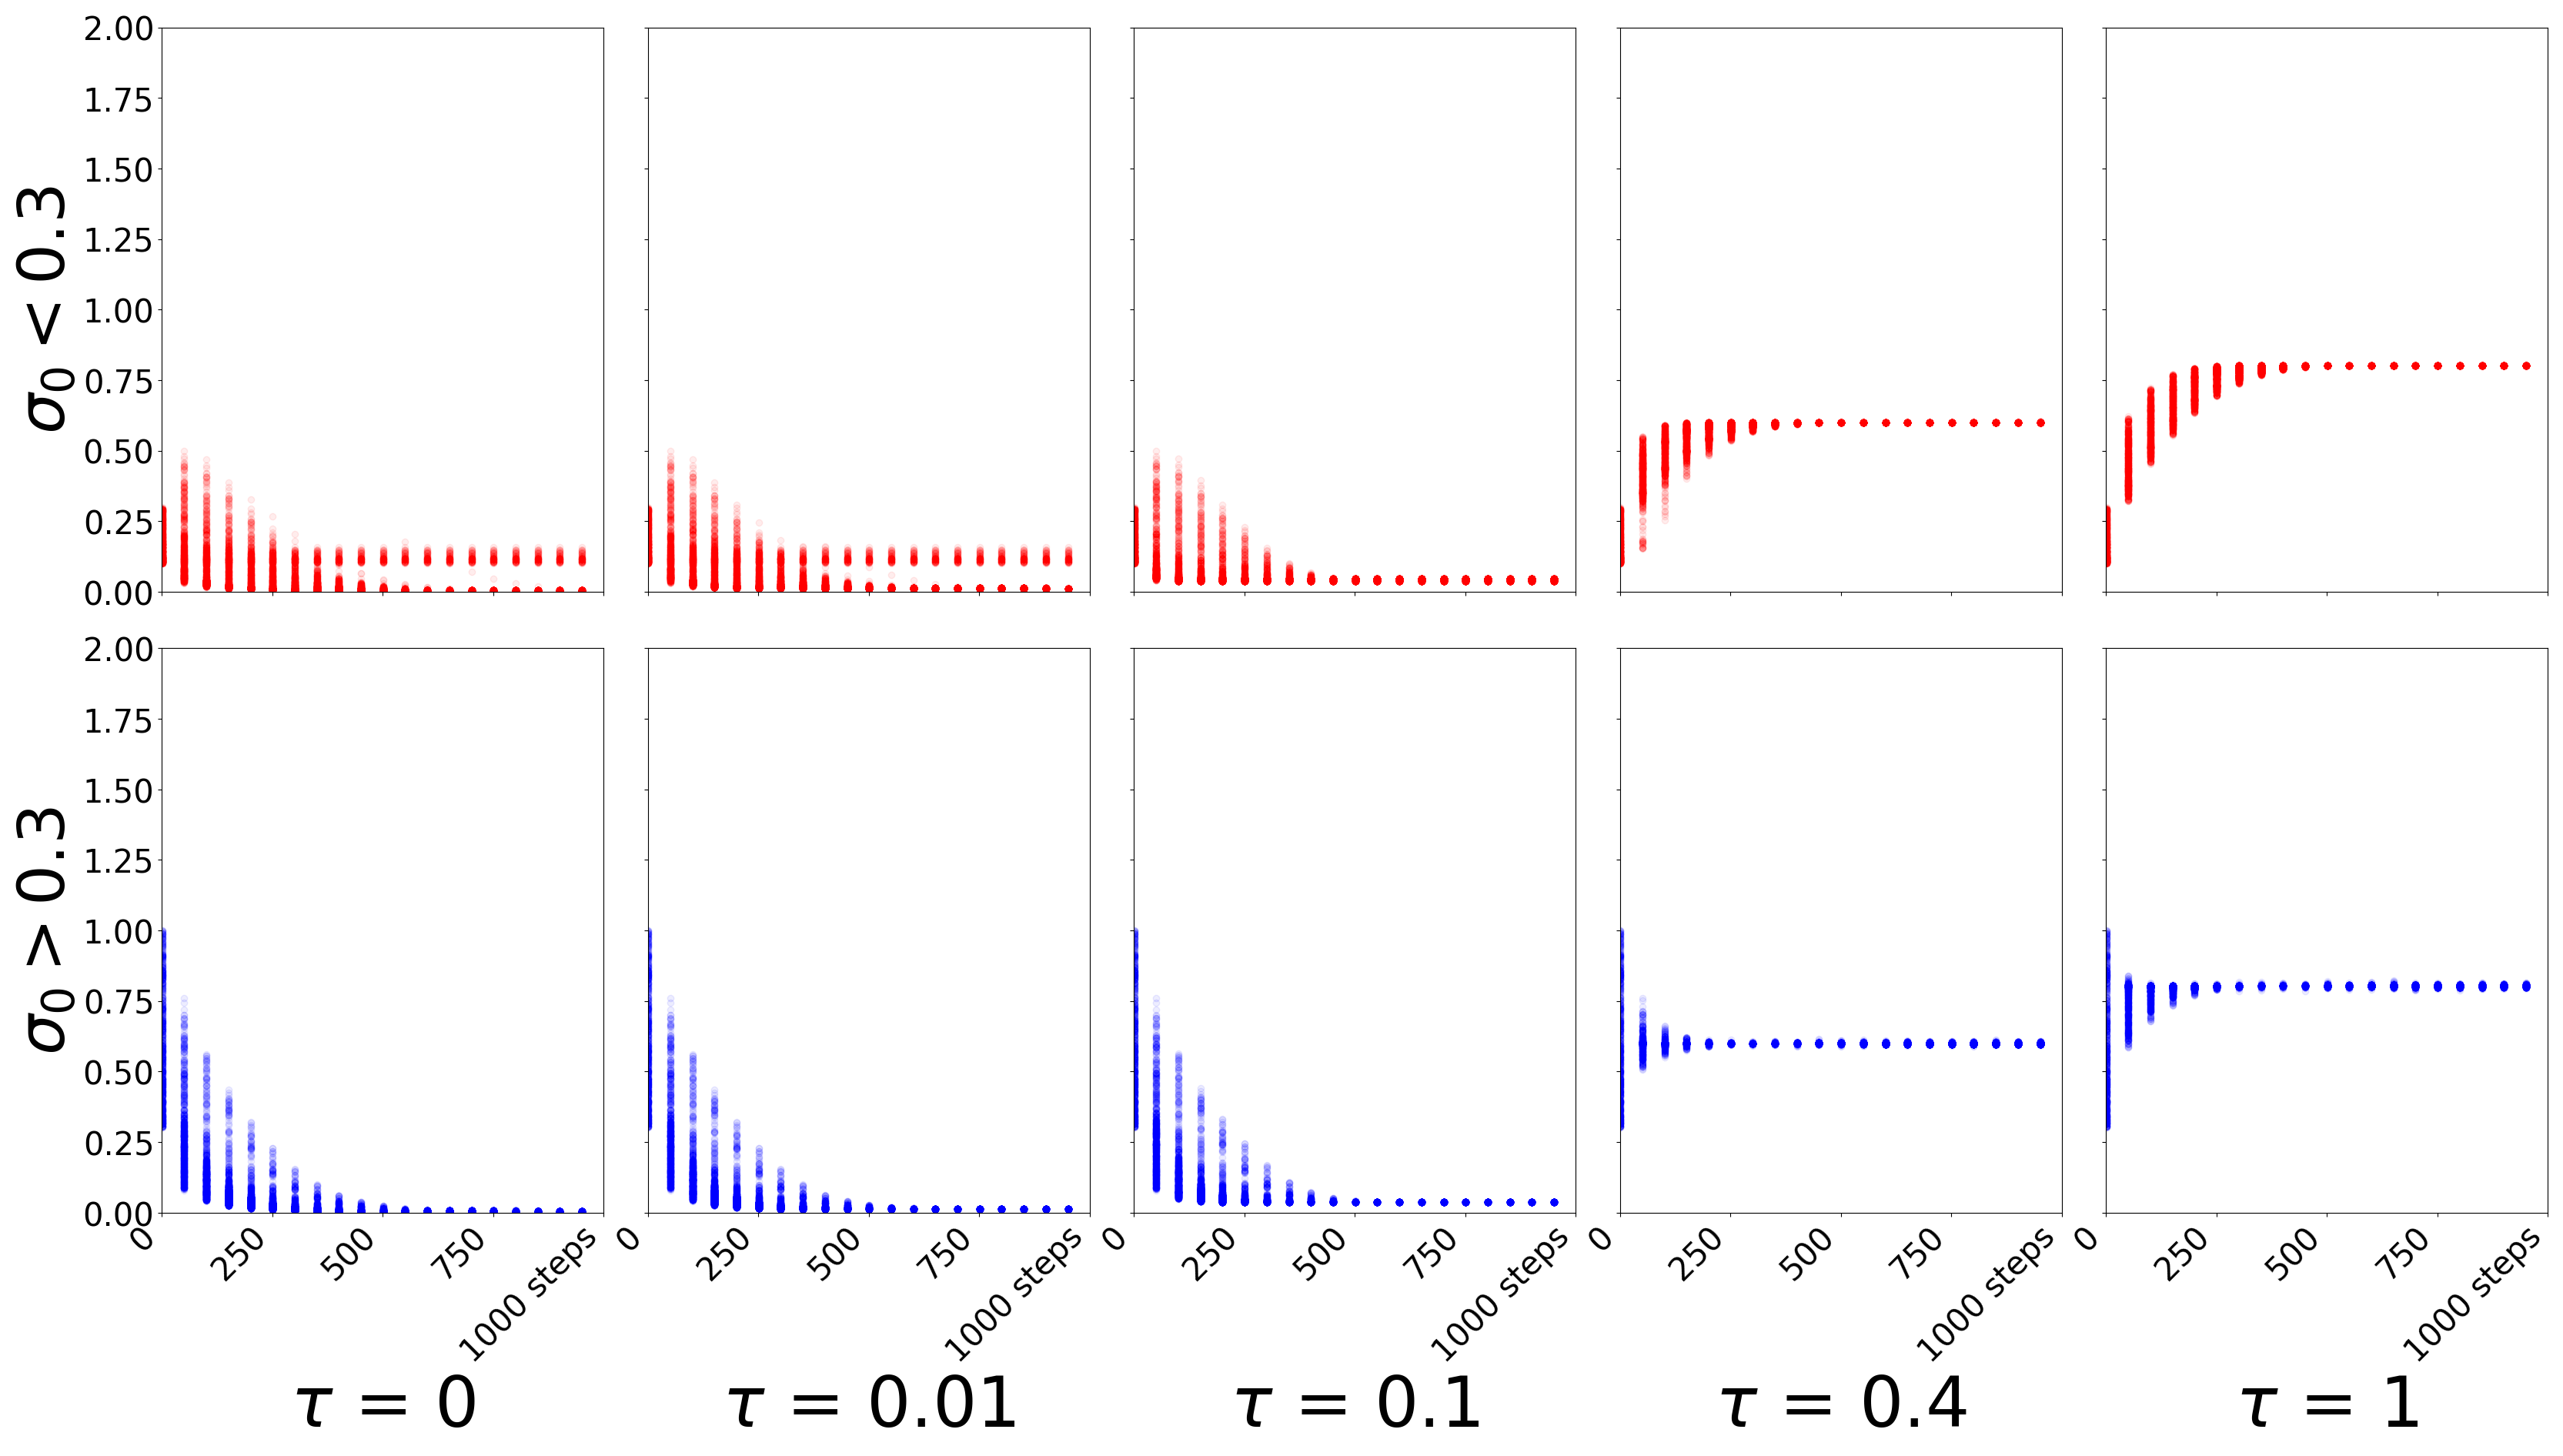
\includegraphics[width=1\columnwidth]{figs/bandit/notlearnQ/modes=1/rmsprop/std_forward_optim=rmsprop_modes=1_lr=0.01.png}
    \caption{Forward KL, RMSprop.}
    \label{fig:bandit-std-forward-rmsprop}
  \end{subfigure}%
  \begin{subfigure}[b]{0.4\linewidth}
    \centering
    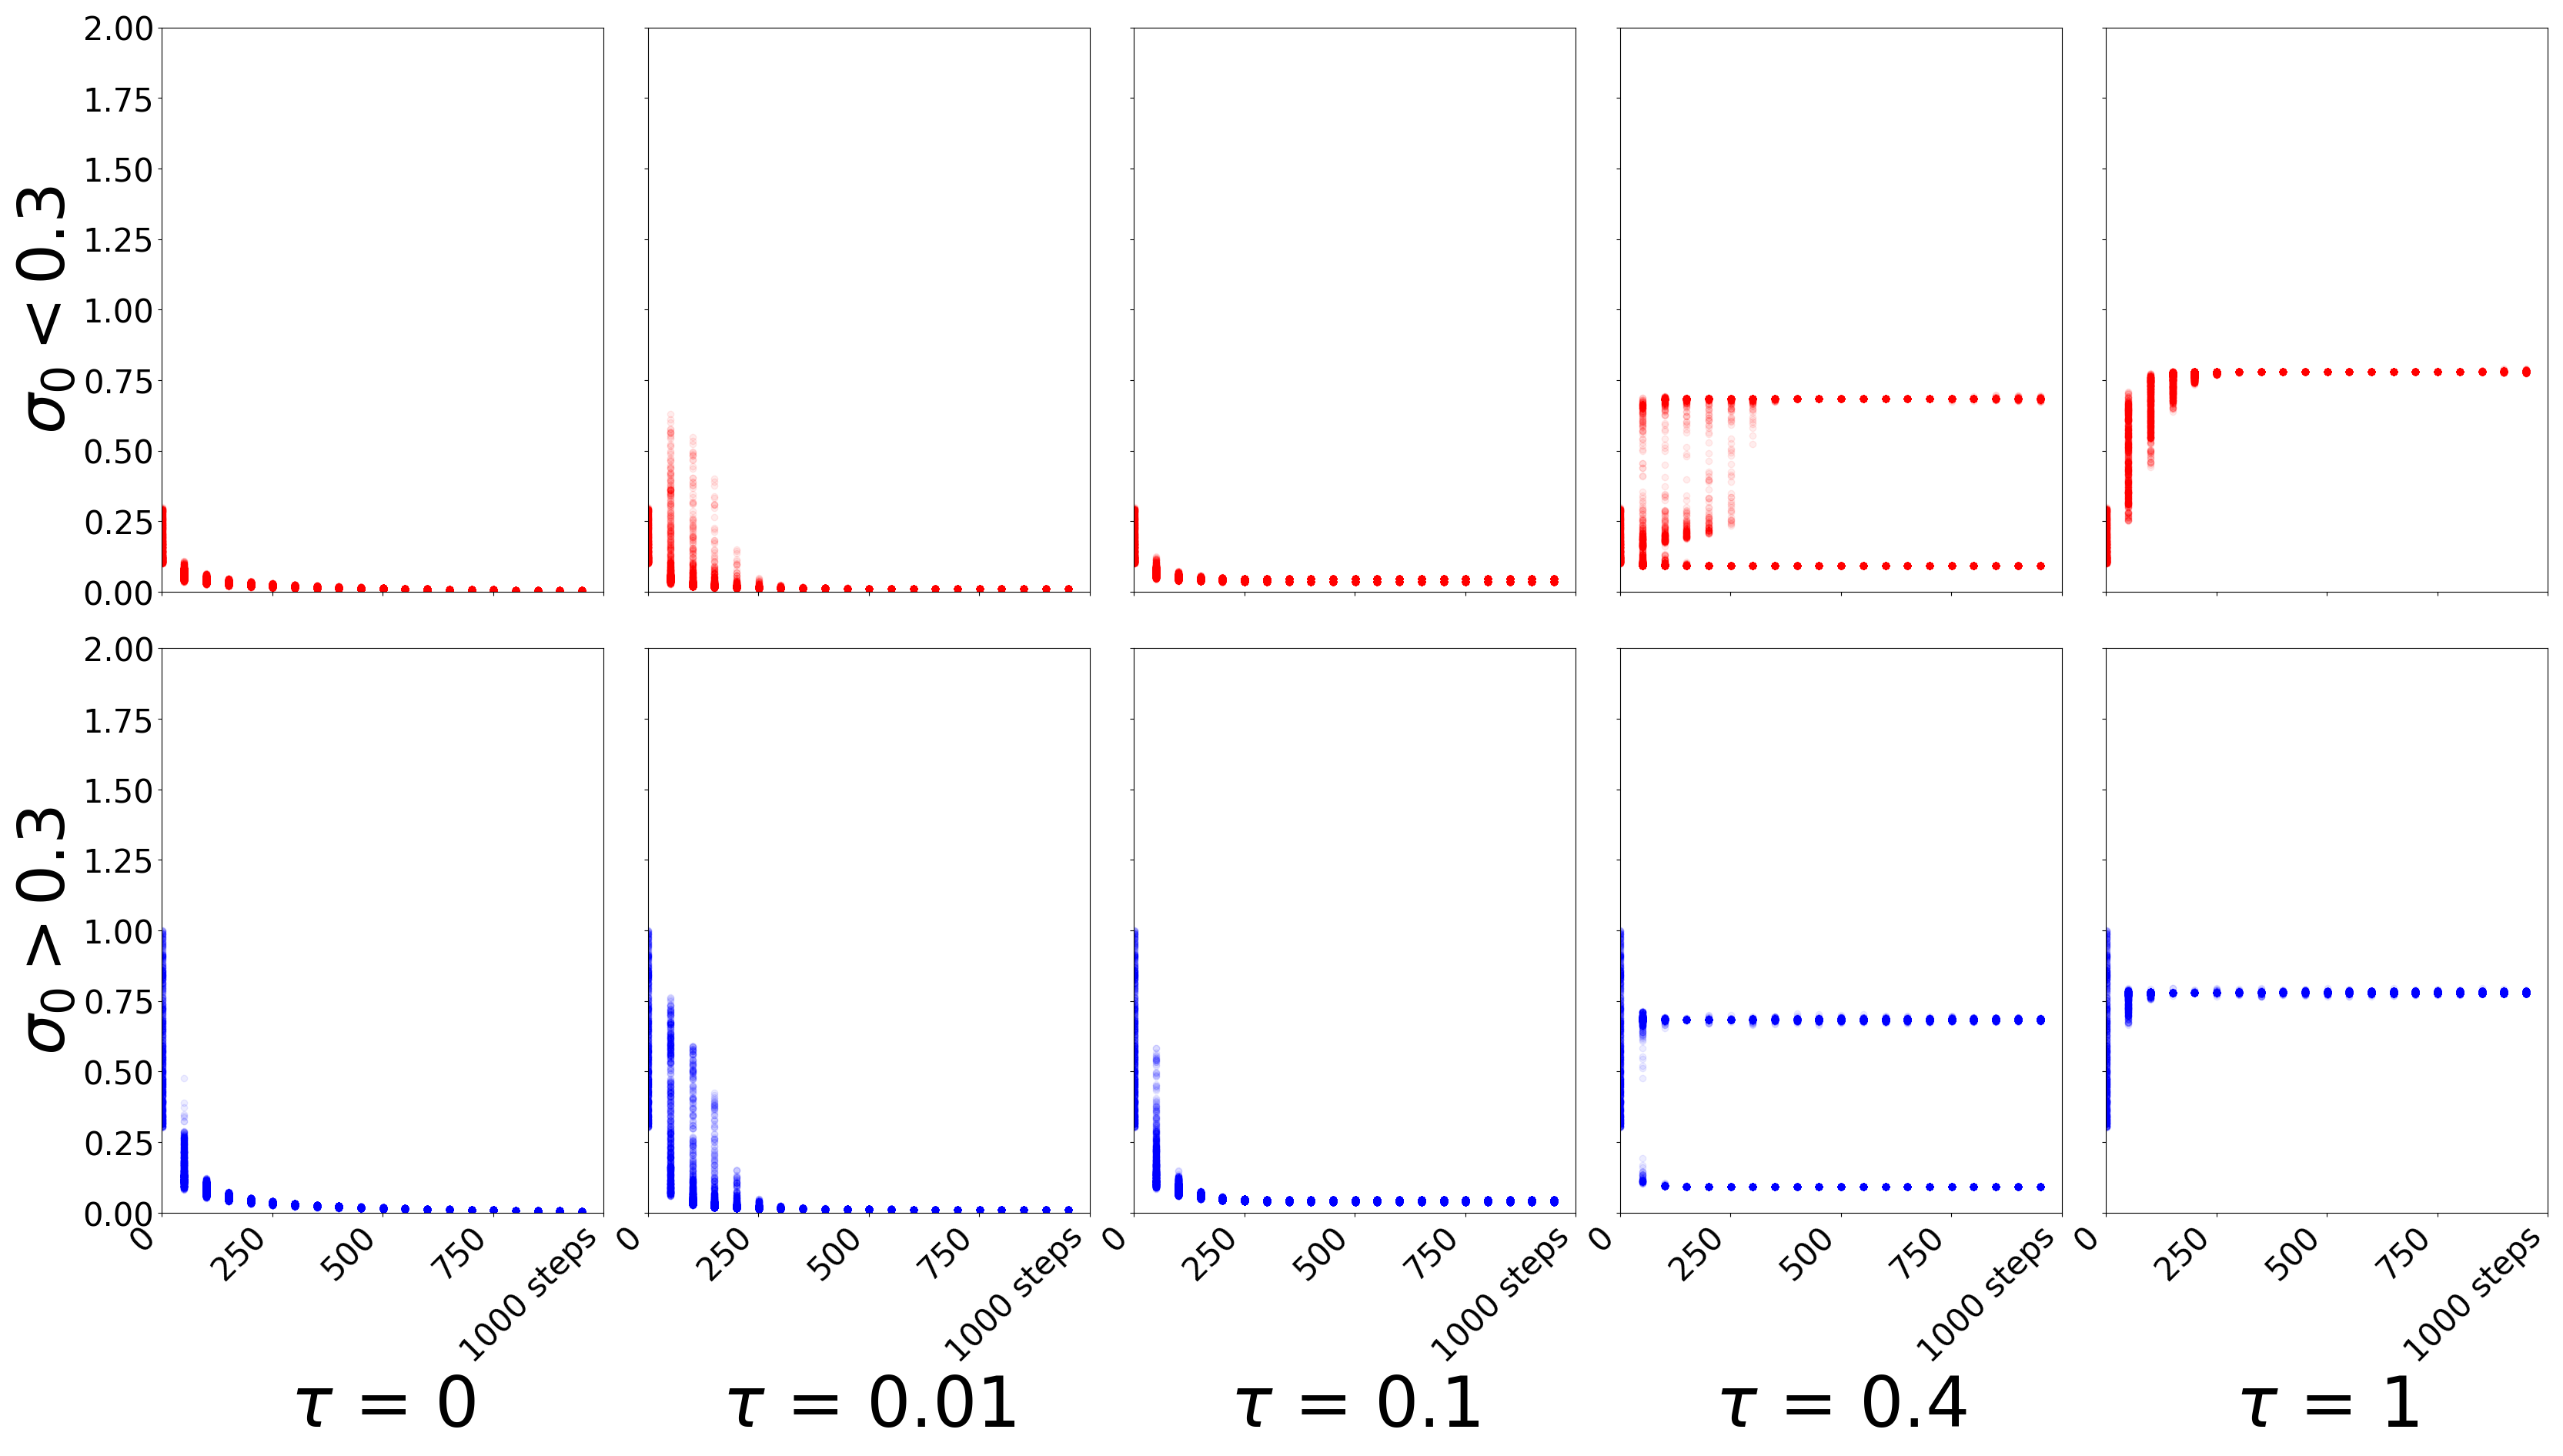
\includegraphics[width=1\columnwidth]{figs/bandit/notlearnQ/modes=1/rmsprop/std_reverse_optim=rmsprop_modes=1_lr=0.01.png}
    \caption{Reverse KL, RMSprop.}
    \label{fig:bandit-std-reverse-rmsprop}
  \end{subfigure}
  
  \begin{subfigure}[b]{0.4\linewidth}
    \centering
    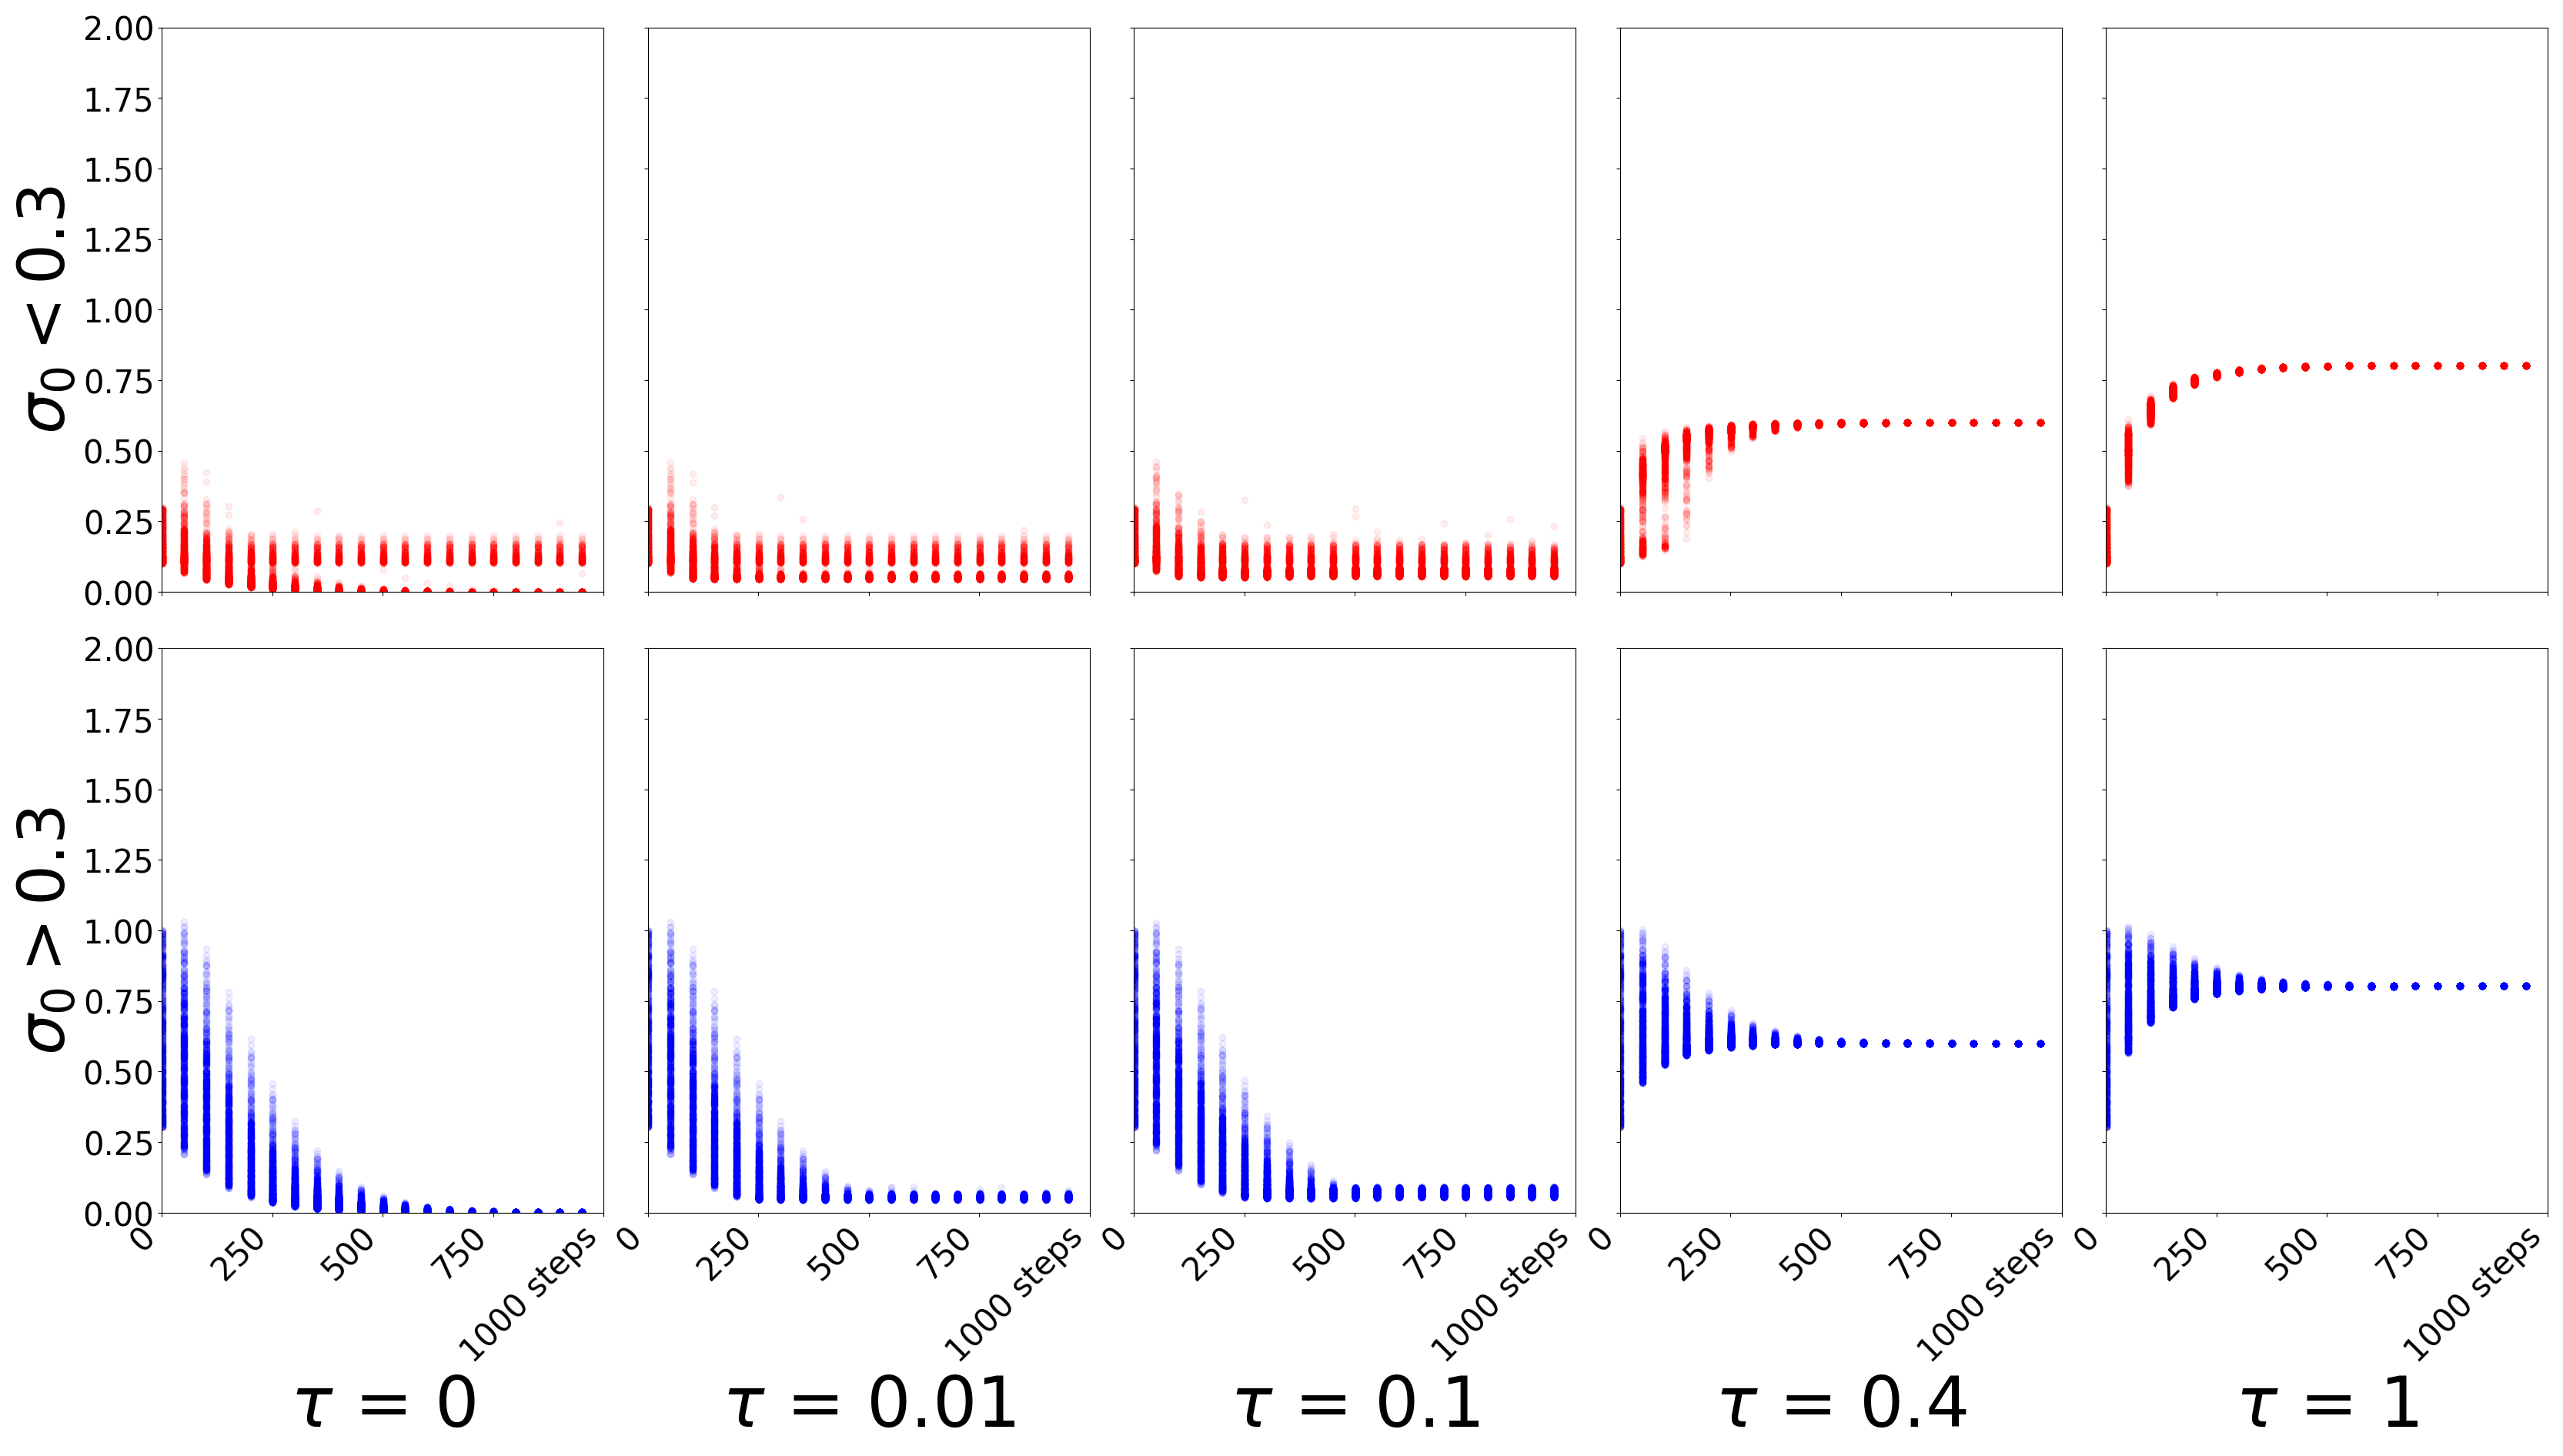
\includegraphics[width=1\columnwidth]{figs/bandit/notlearnQ/modes=1/sgd/std_forward_optim=sgd_modes=1_lr=0.01.png}
    \caption{Forward KL, SGD.}
    \label{fig:bandit-std-forward-sgd}
  \end{subfigure}%
  \begin{subfigure}[b]{0.4\linewidth}
    \centering
    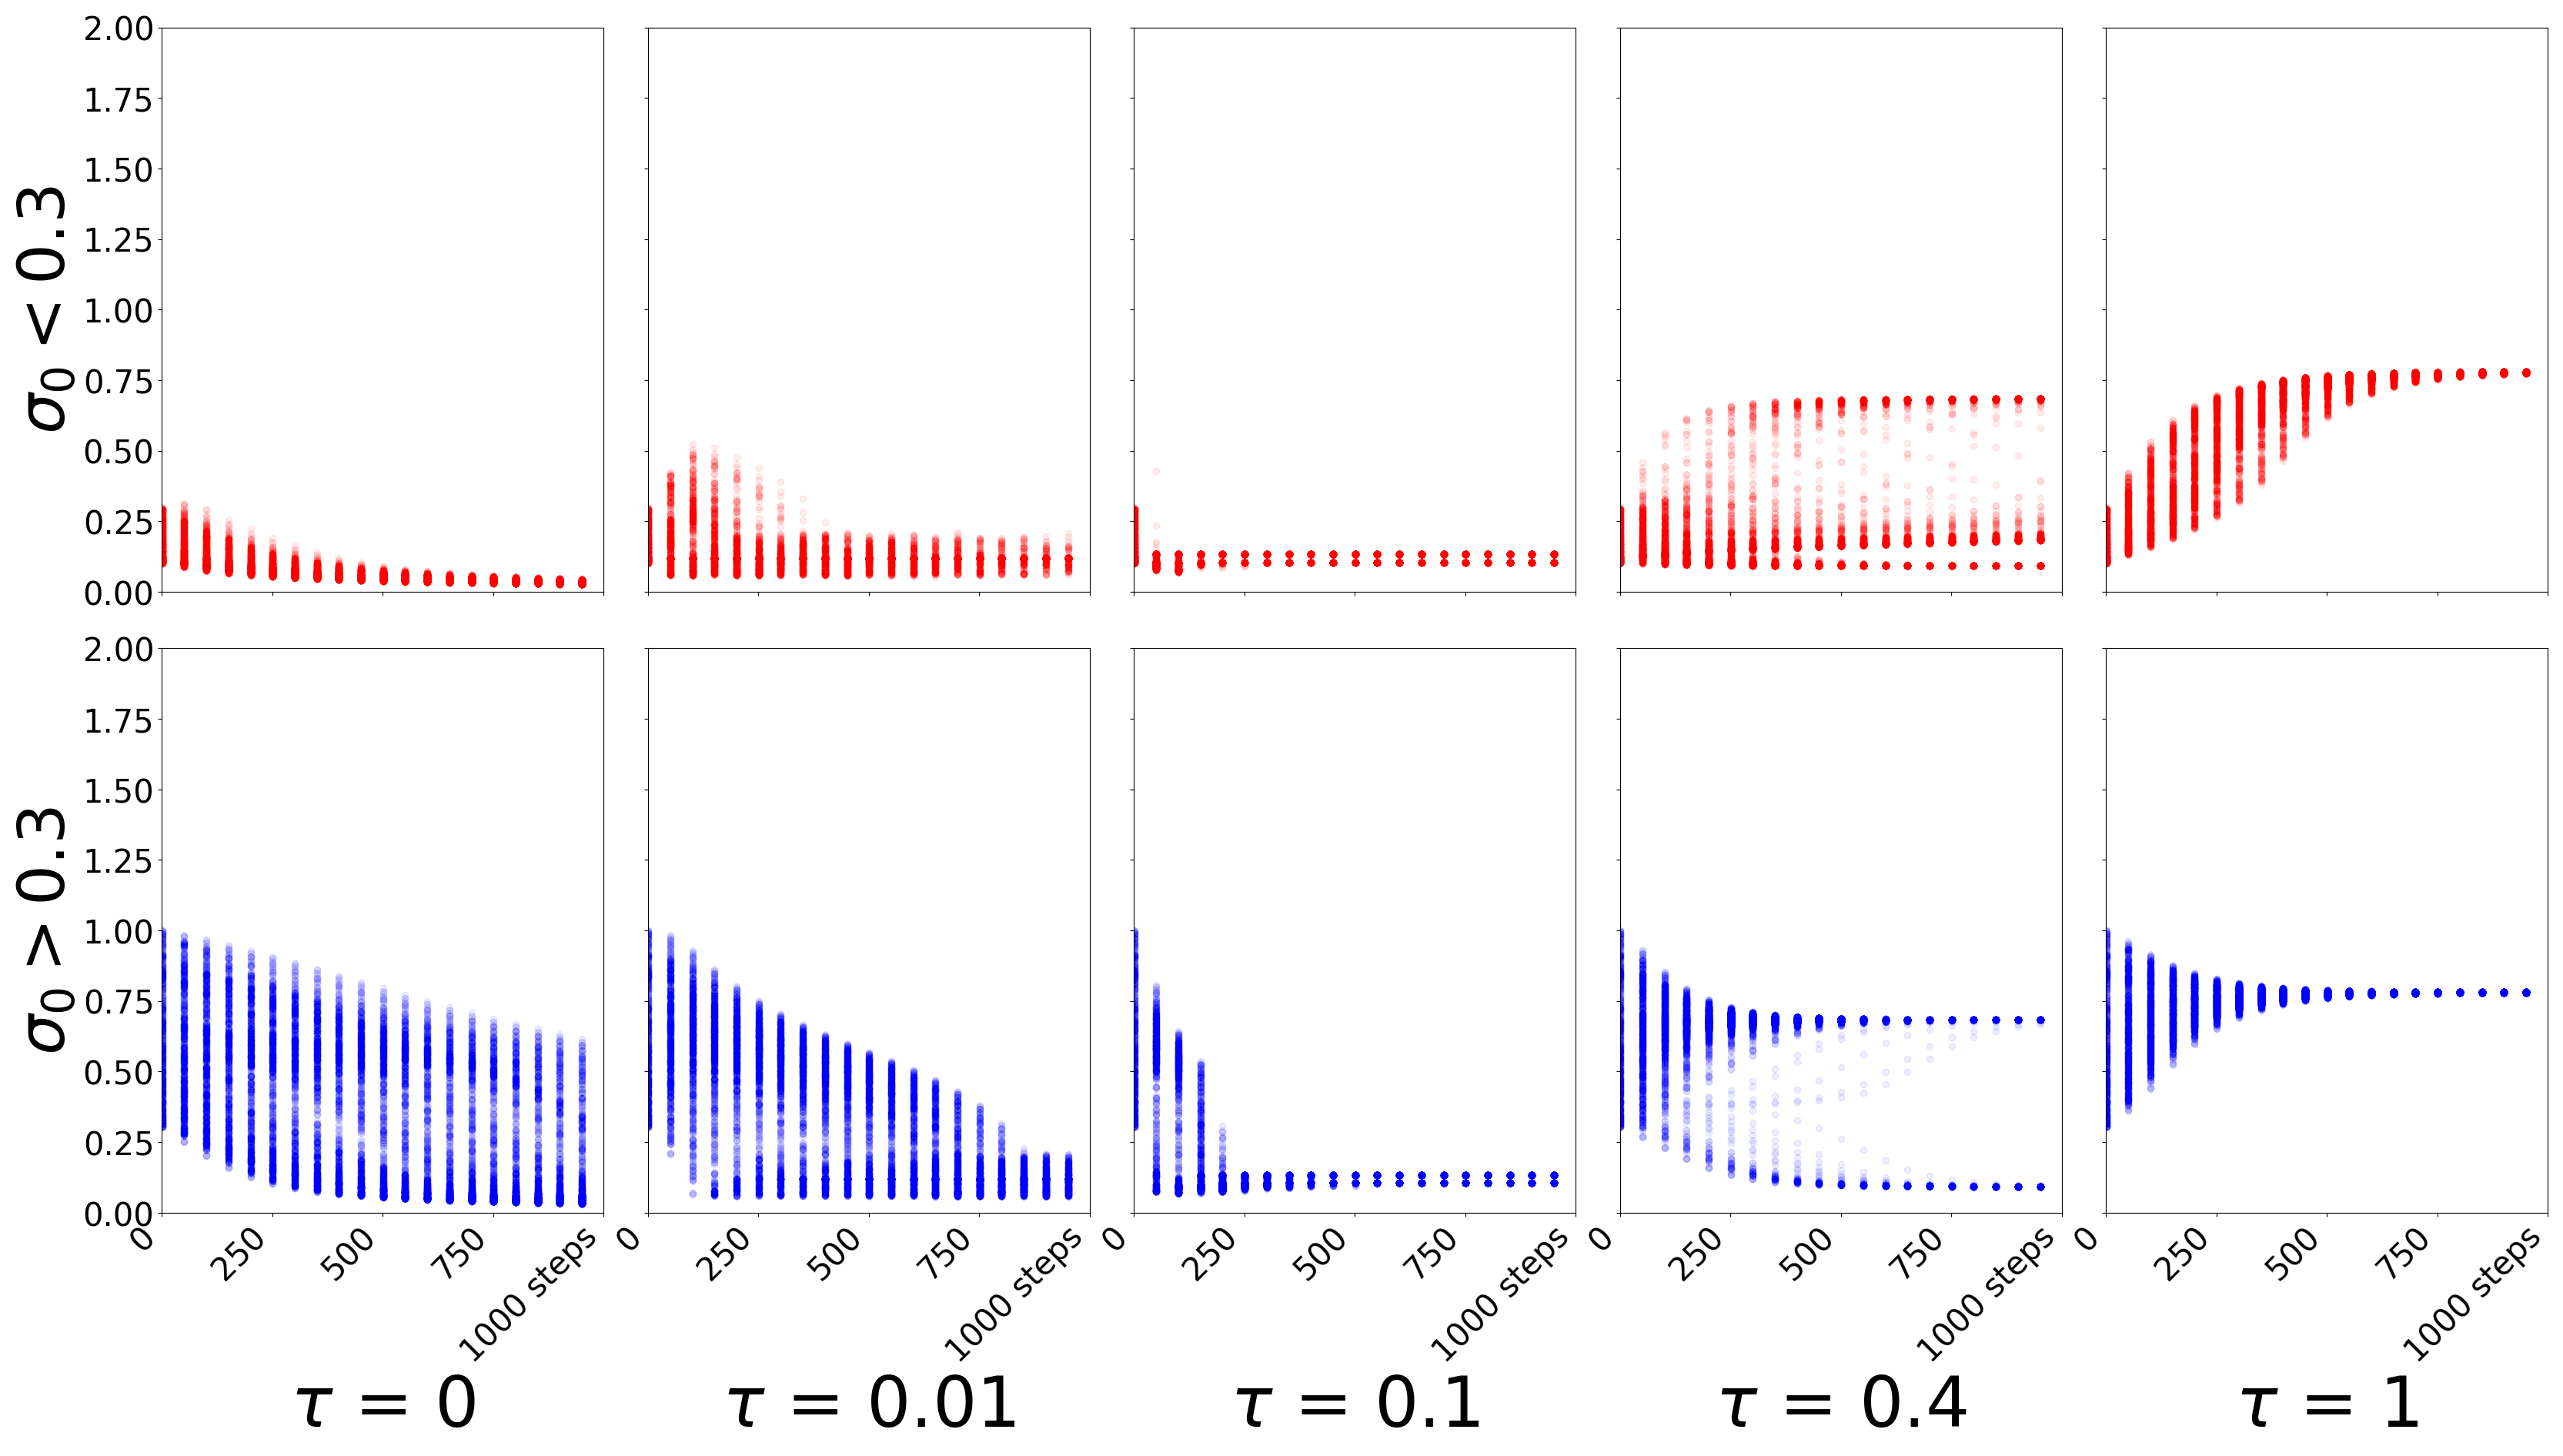
\includegraphics[width=1\columnwidth]{figs/bandit/notlearnQ/modes=1/sgd/std_reverse_optim=sgd_modes=1_lr=0.01.png}
    \caption{Reverse KL, SGD.}
    \label{fig:bandit-std-reverse-sgd}
  \end{subfigure}
  \caption{Standard deviation over time with unimodal policy. }
\end{figure}


\begin{figure}[!ht]
  \centering
  \begin{subfigure}[b]{0.4\linewidth}
    \centering
    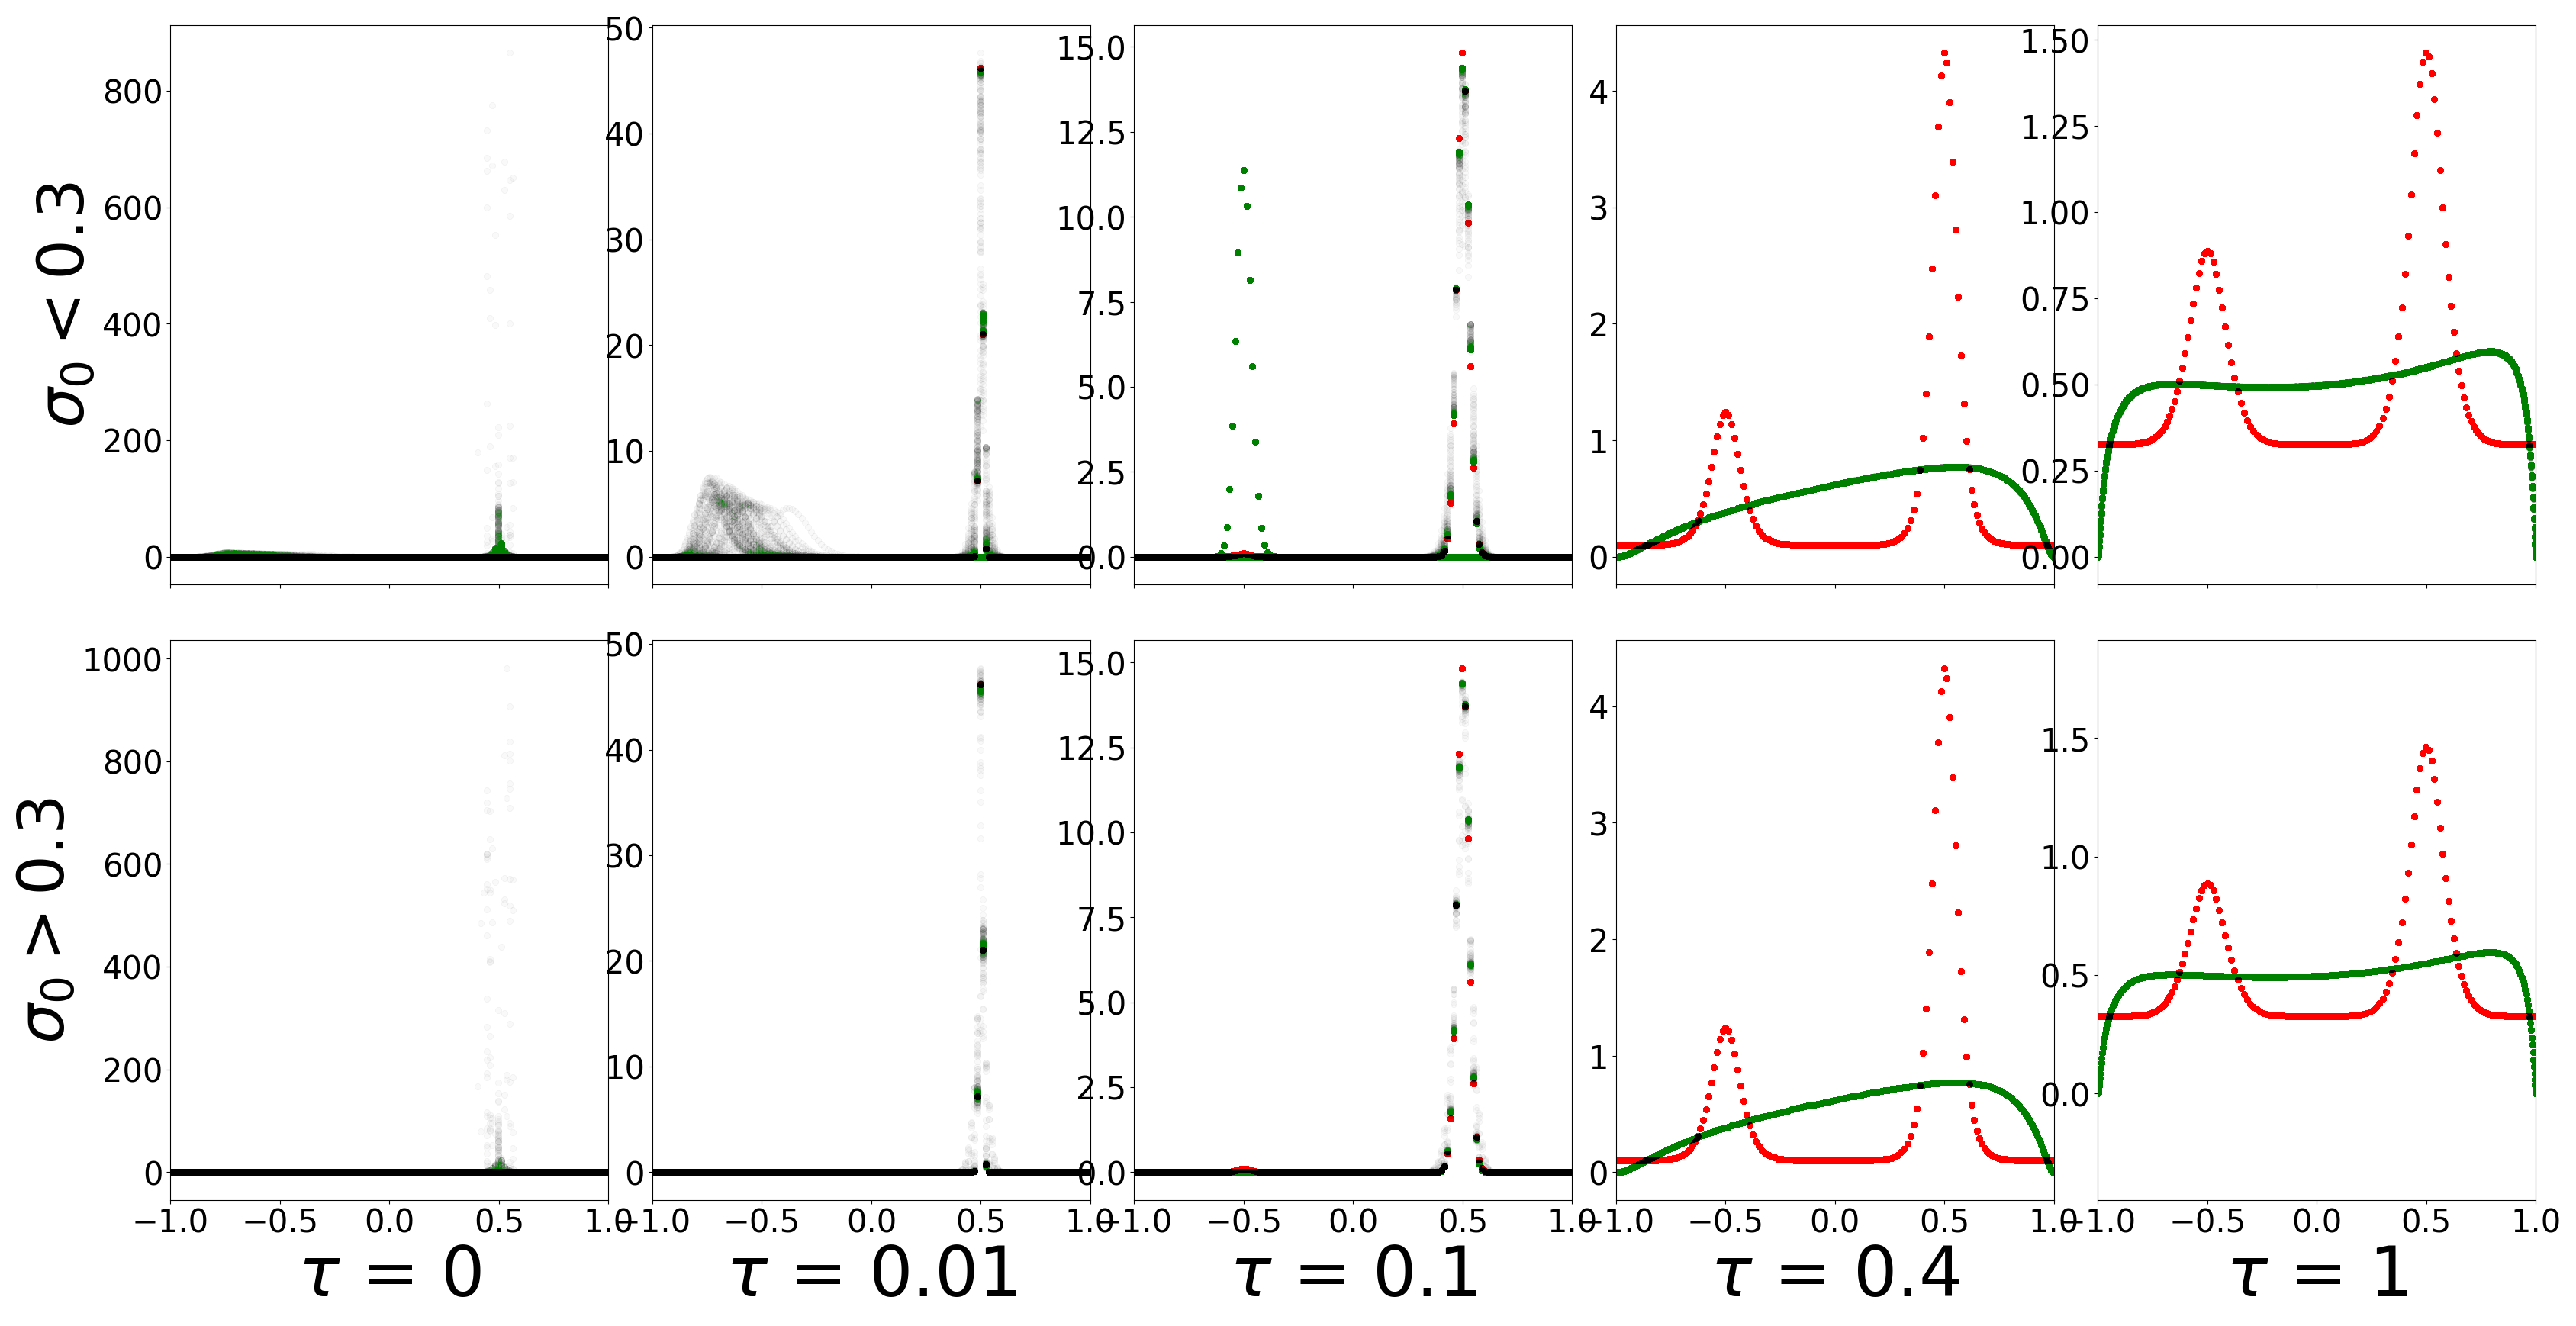
\includegraphics[width=1\columnwidth]{figs/bandit/notlearnQ/modes=1/adam/pdf_forward_optim=adam_modes=1_lr=0.01.png}
    \caption{Forward KL, Adam.}
    \label{fig:bandit-pdf-forward-adam}
  \end{subfigure}%
  \begin{subfigure}[b]{0.4\linewidth}
    \centering
    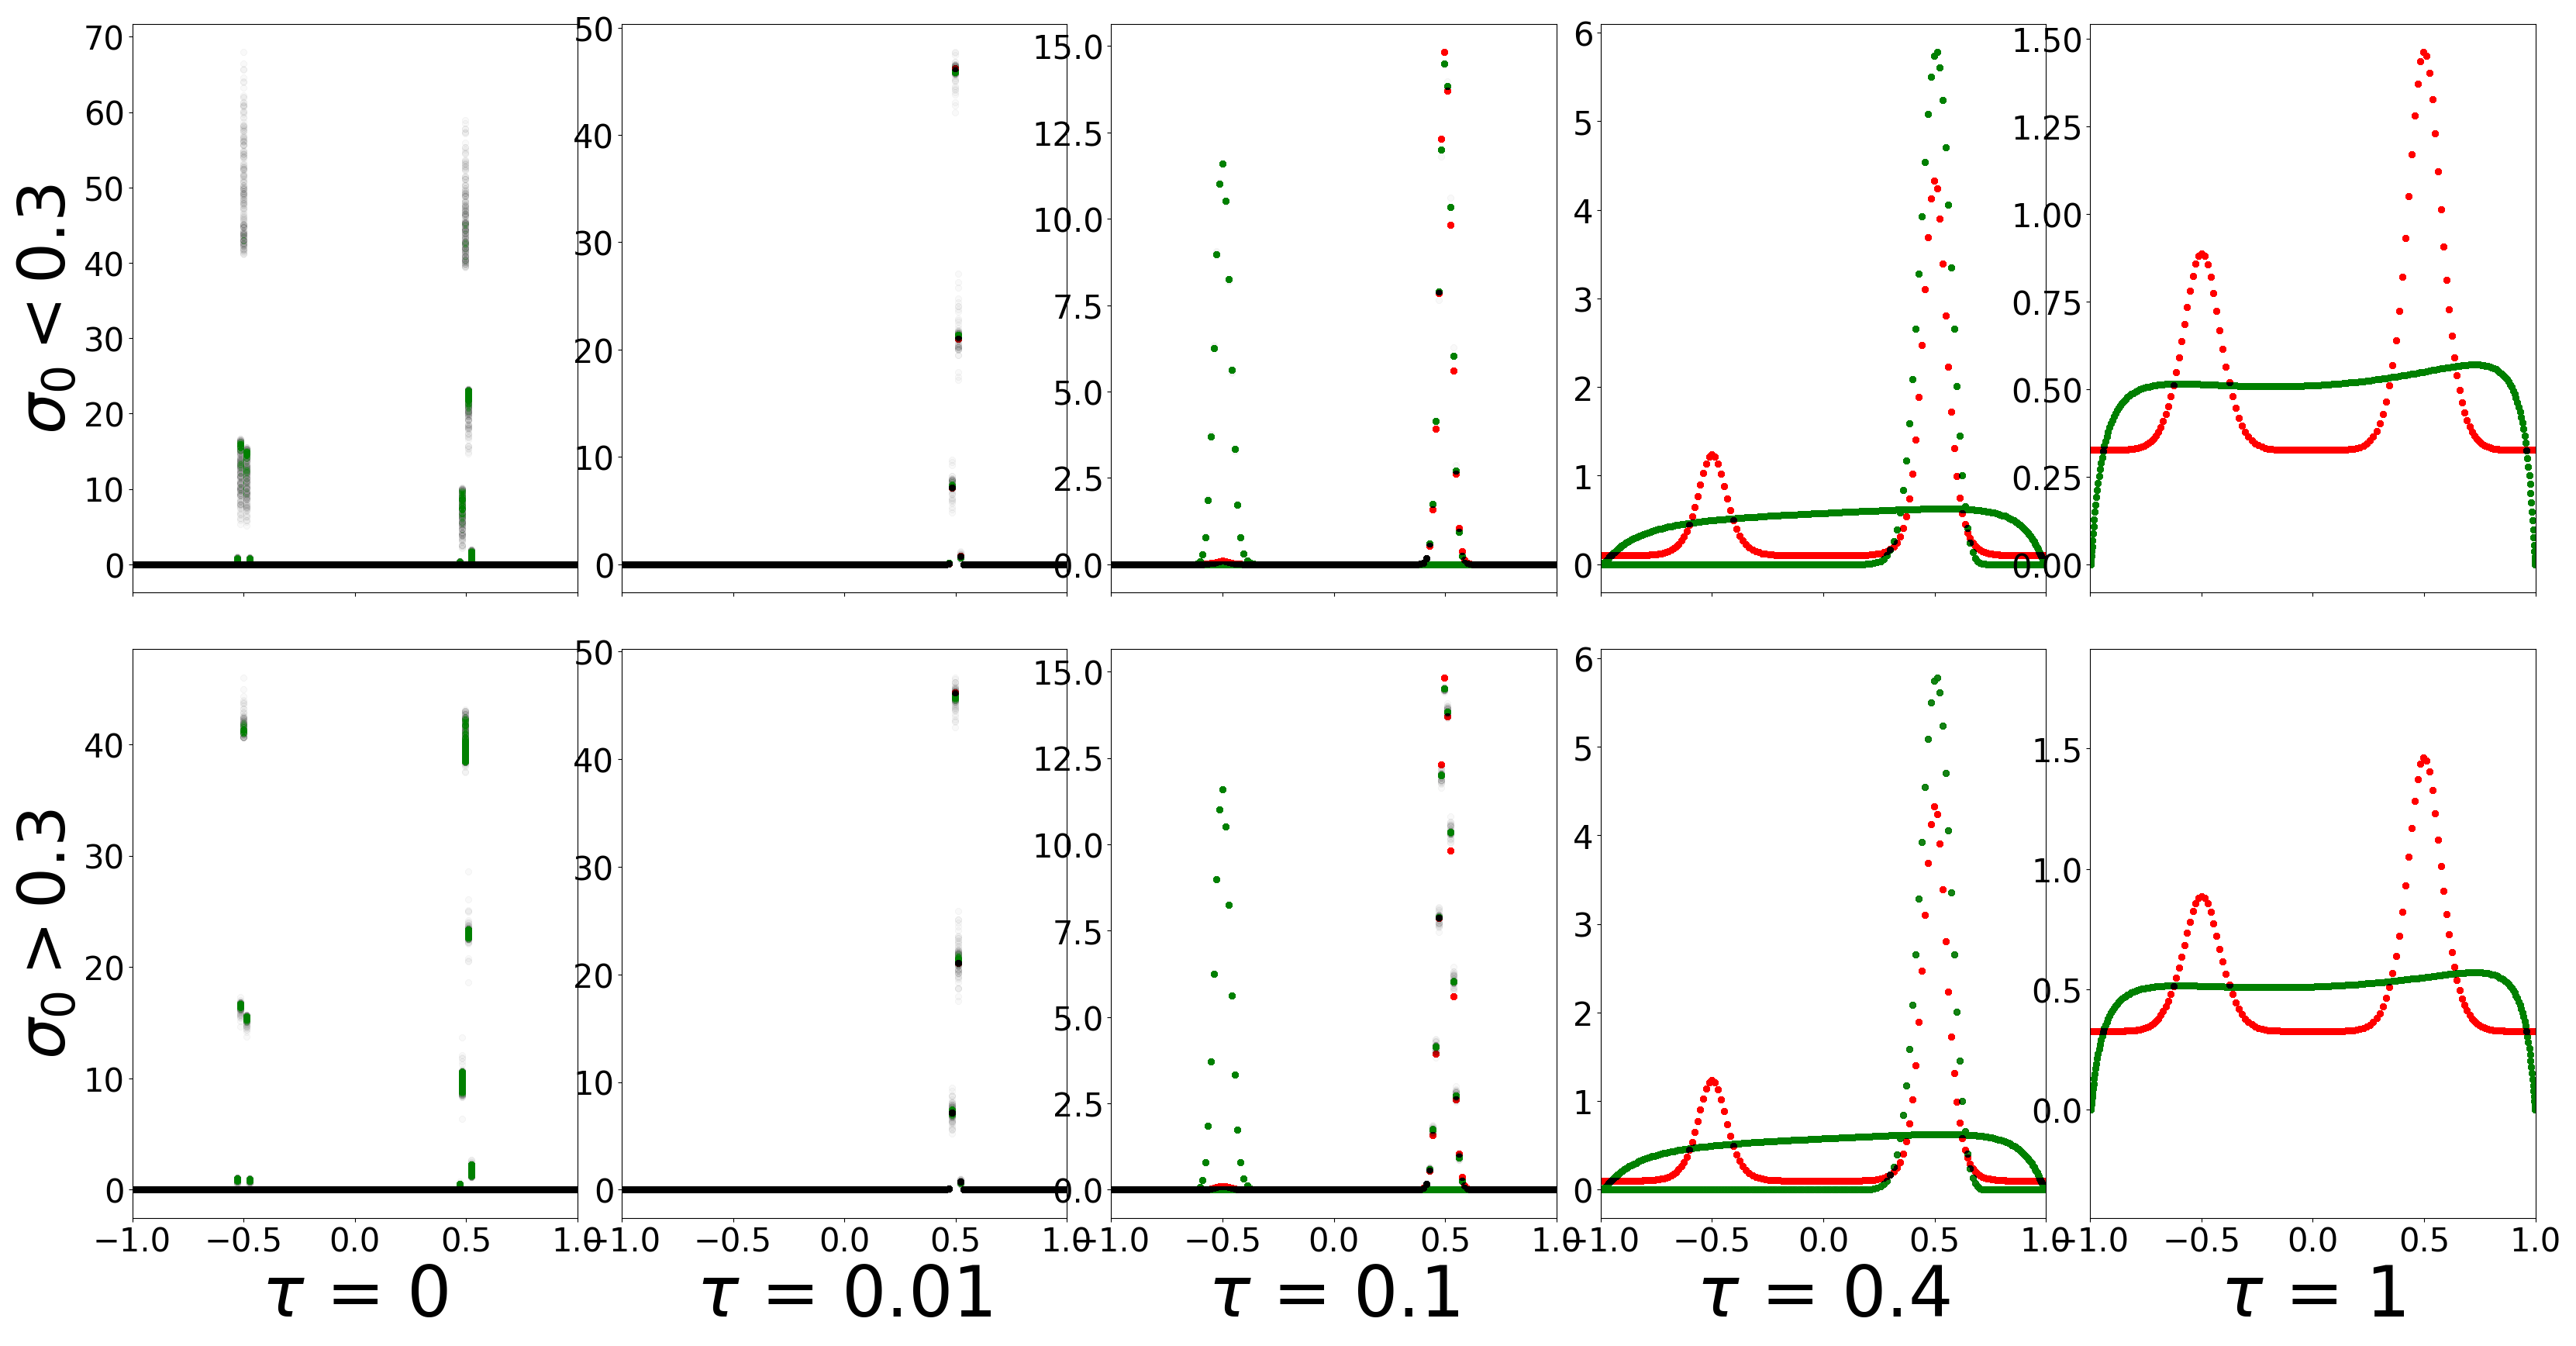
\includegraphics[width=1\columnwidth]{figs/bandit/notlearnQ/modes=1/adam/pdf_reverse_optim=adam_modes=1_lr=0.01.png}
    \caption{Reverse KL, Adam. }
    \label{fig:bandit-pdf-reverse-adam}
  \end{subfigure}
  
  \begin{subfigure}[b]{0.4\linewidth}
    \centering
    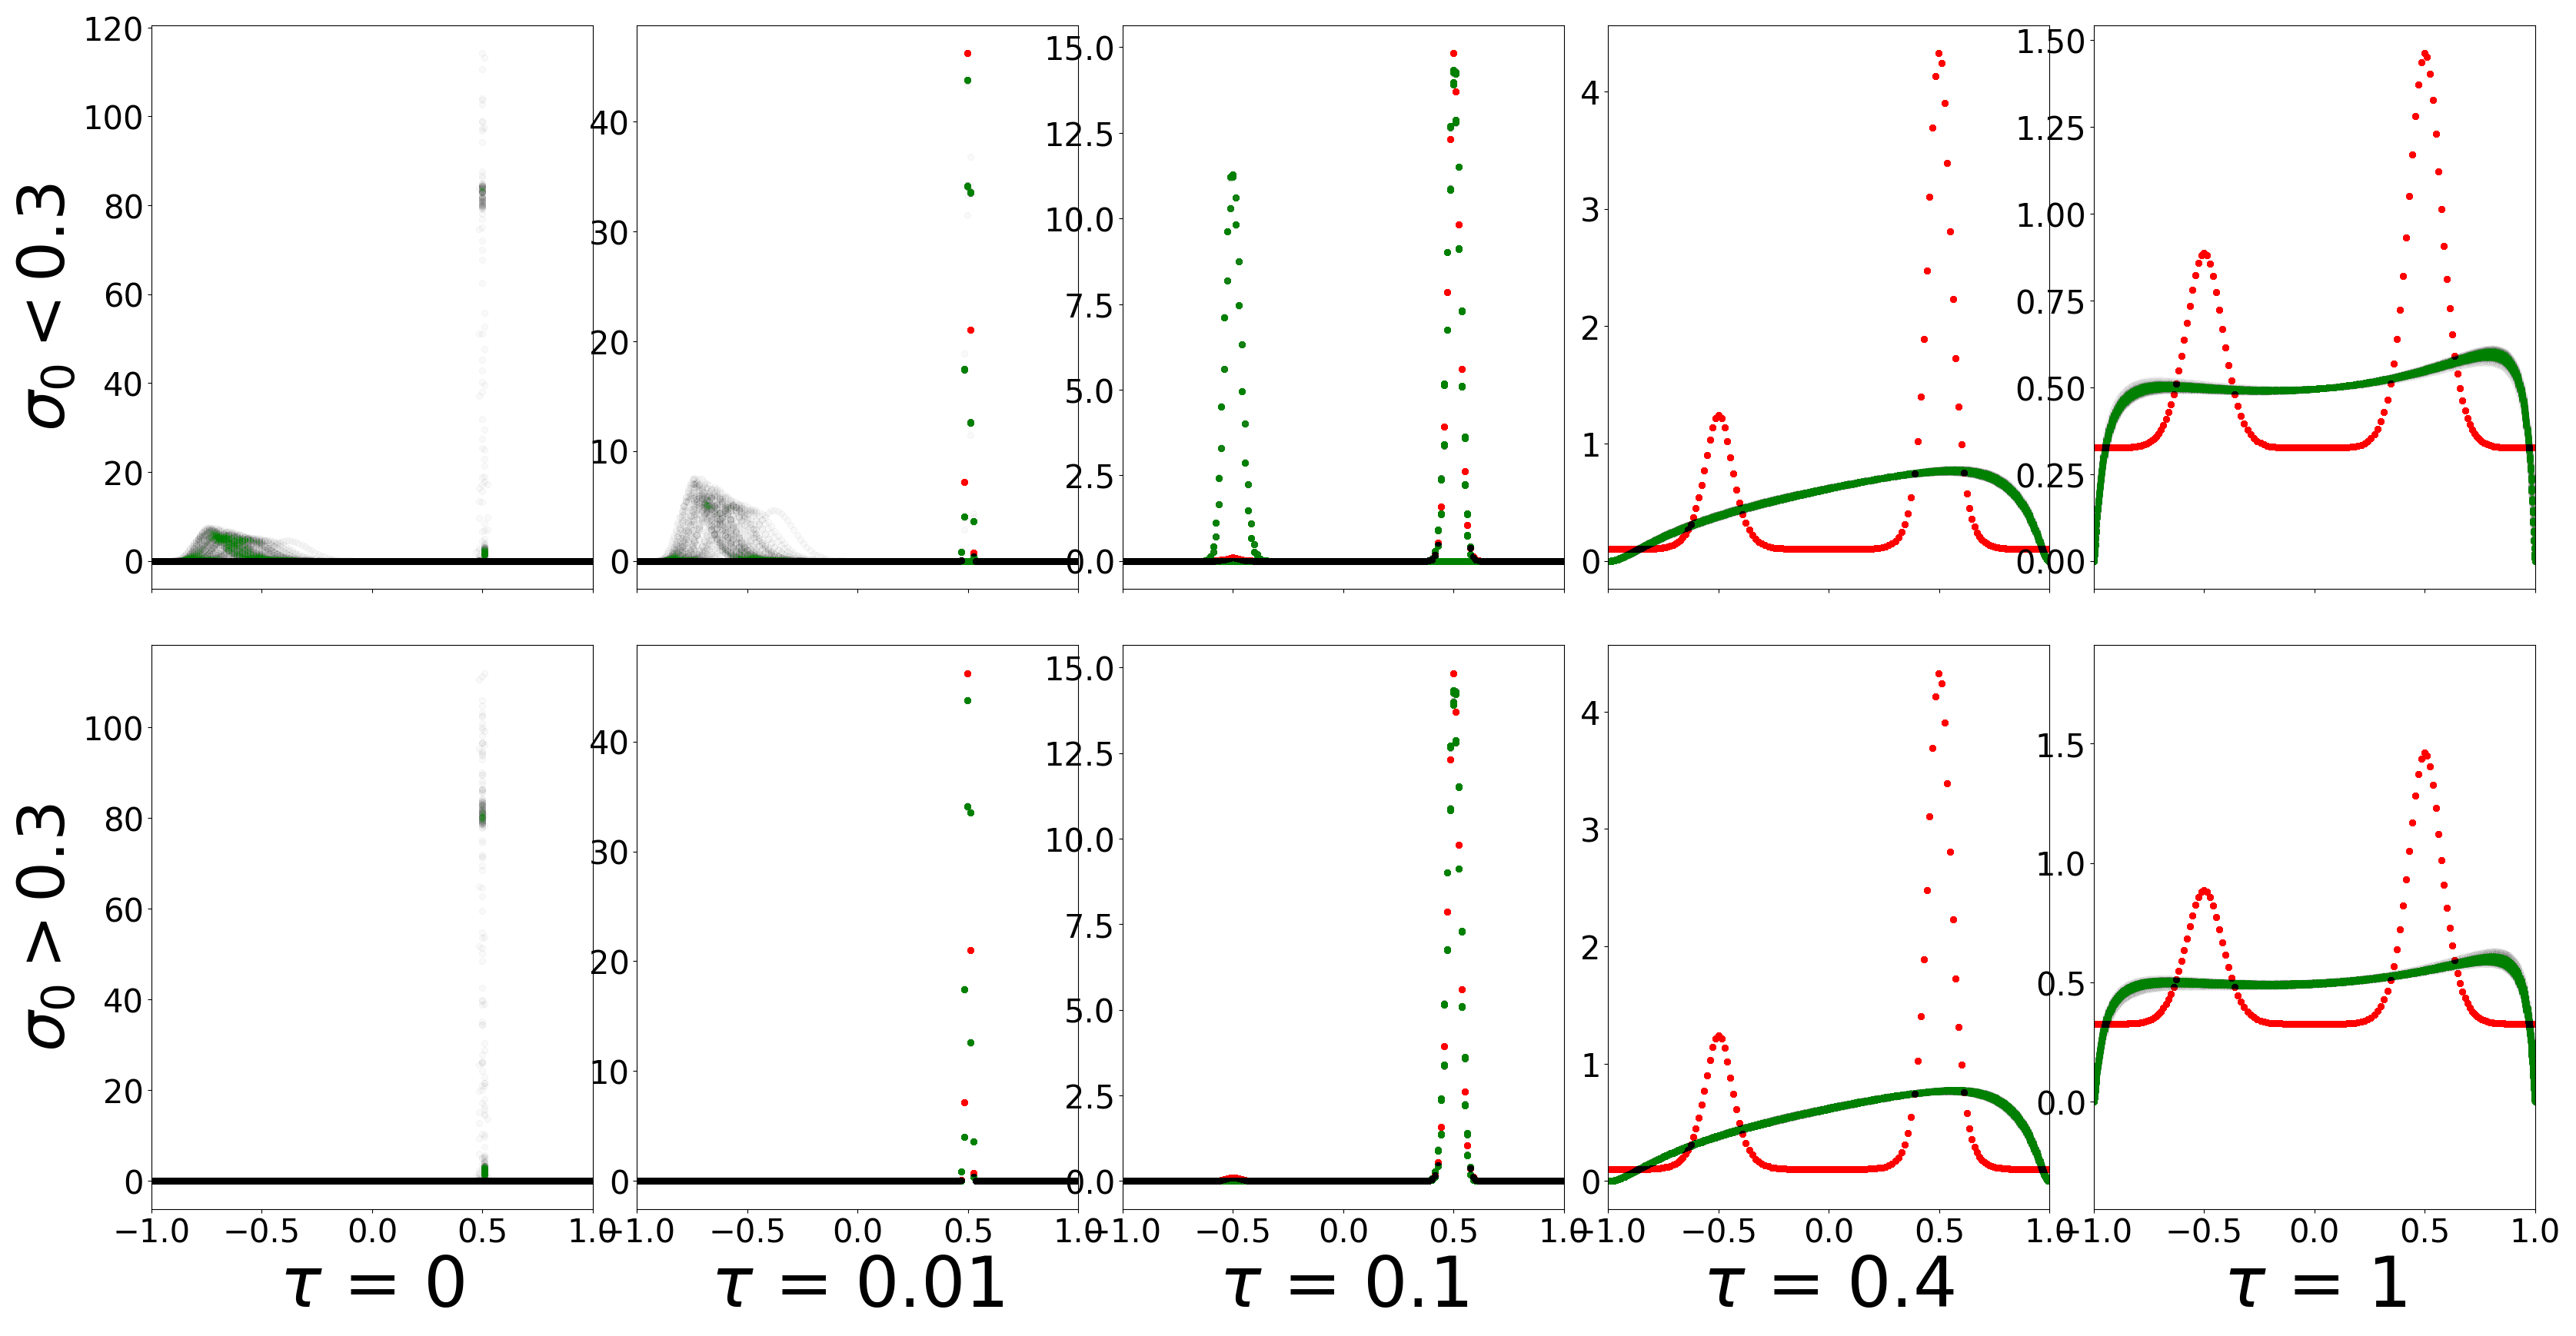
\includegraphics[width=1\columnwidth]{figs/bandit/notlearnQ/modes=1/rmsprop/pdf_forward_optim=rmsprop_modes=1_lr=0.01.png}
    \caption{Forward KL, RMSprop.}
    \label{fig:bandit-pdf-forward-rmsprop}
  \end{subfigure}%
  \begin{subfigure}[b]{0.4\linewidth}
    \centering
    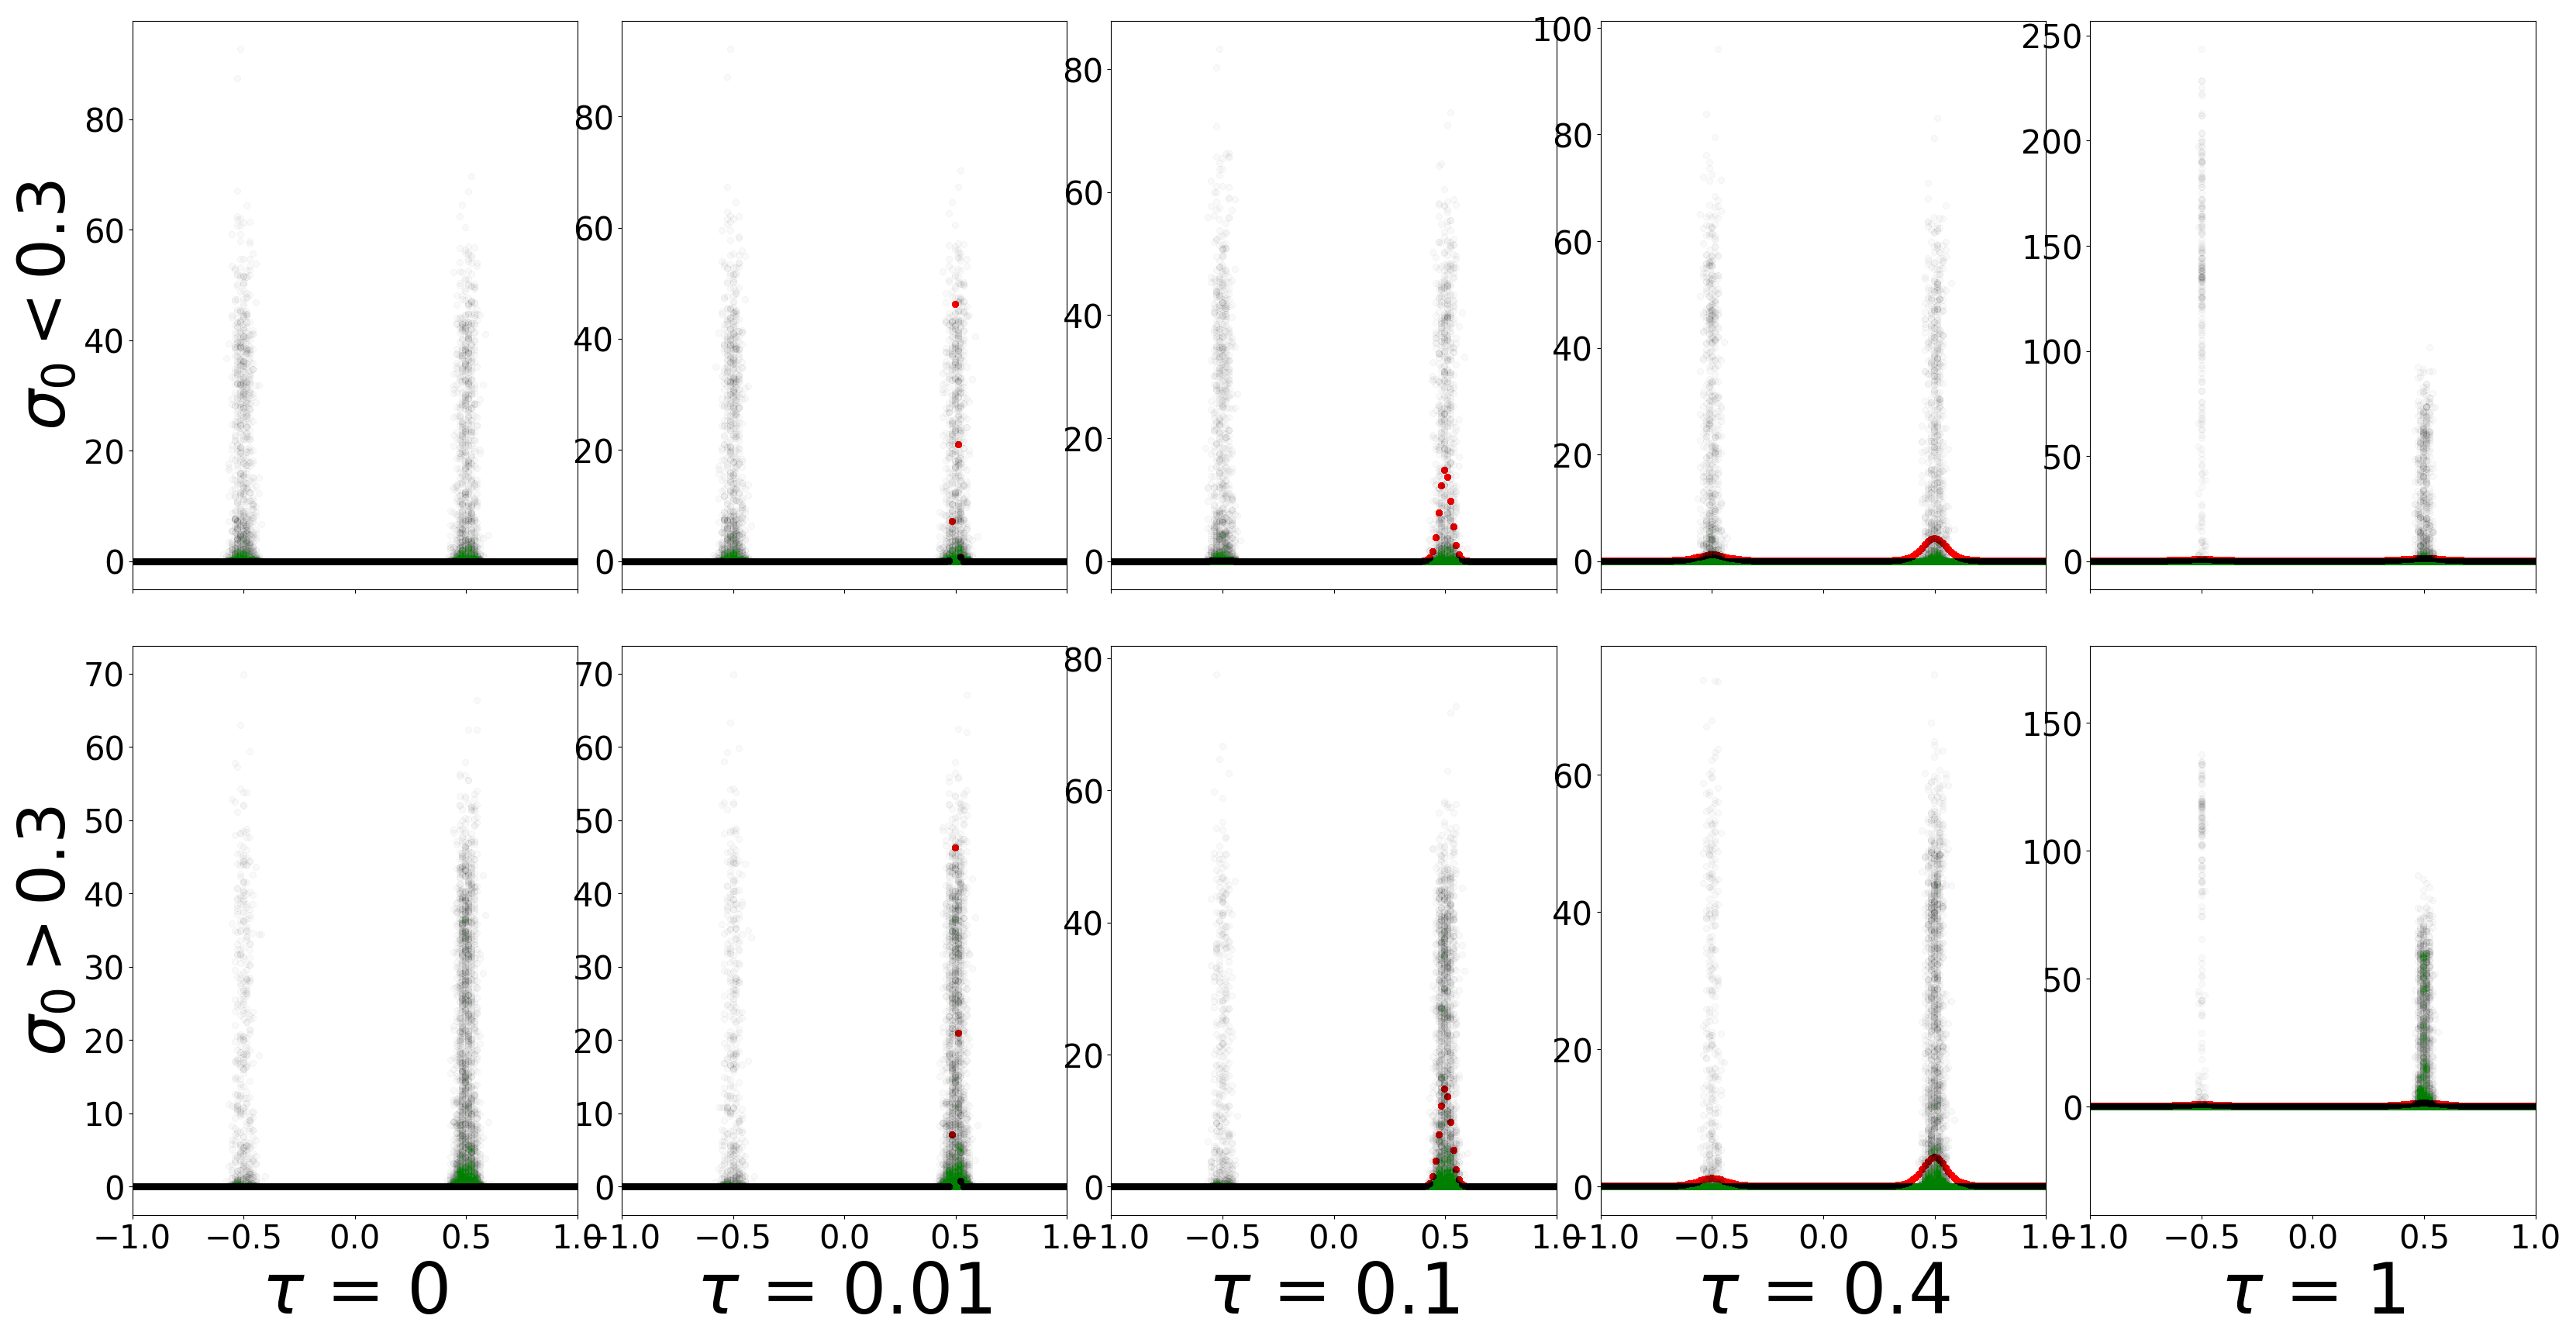
\includegraphics[width=1\columnwidth]{figs/bandit/notlearnQ/modes=1/rmsprop/pdf_reverse_optim=rmsprop_modes=1_lr=0.01.png}
    \caption{Reverse KL, RMSprop.}
    \label{fig:bandit-pdf-reverse-rmsprop}
  \end{subfigure}
  
  \begin{subfigure}[b]{0.4\linewidth}
    \centering
    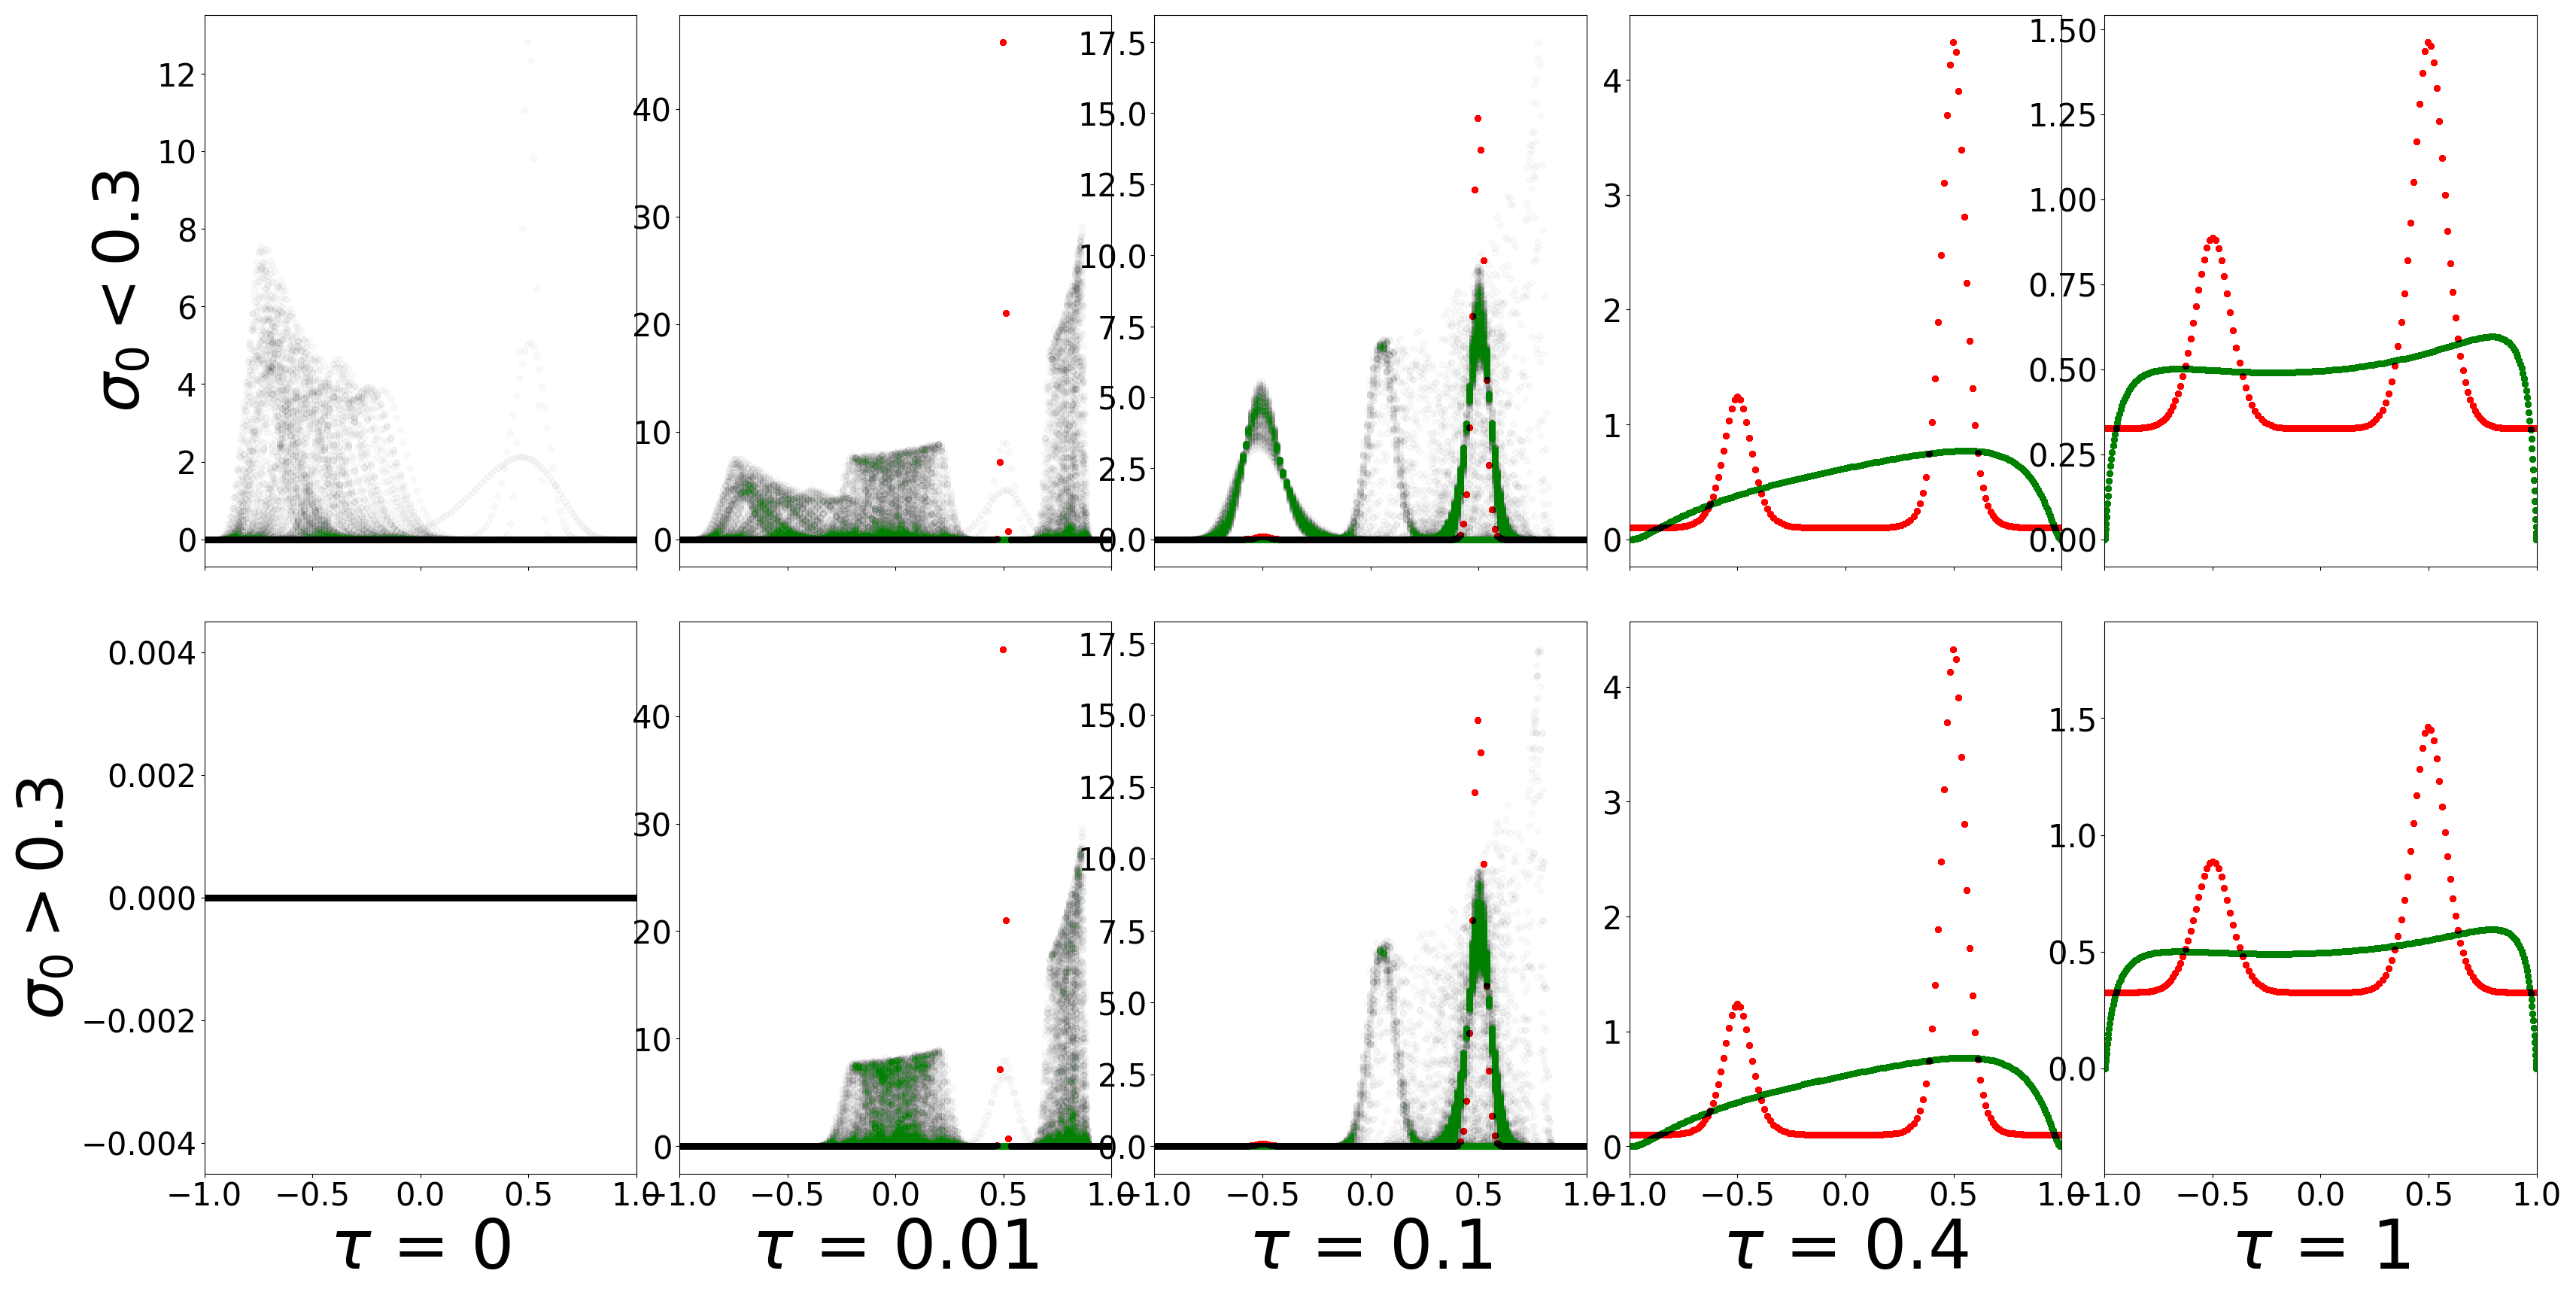
\includegraphics[width=1\columnwidth]{figs/bandit/notlearnQ/modes=1/sgd/pdf_forward_optim=sgd_modes=1_lr=0.01.png}
    \caption{Forward KL, SGD.}
    \label{fig:bandit-pdf-forward-sgd}
  \end{subfigure}%
  \begin{subfigure}[b]{0.4\linewidth}
    \centering
    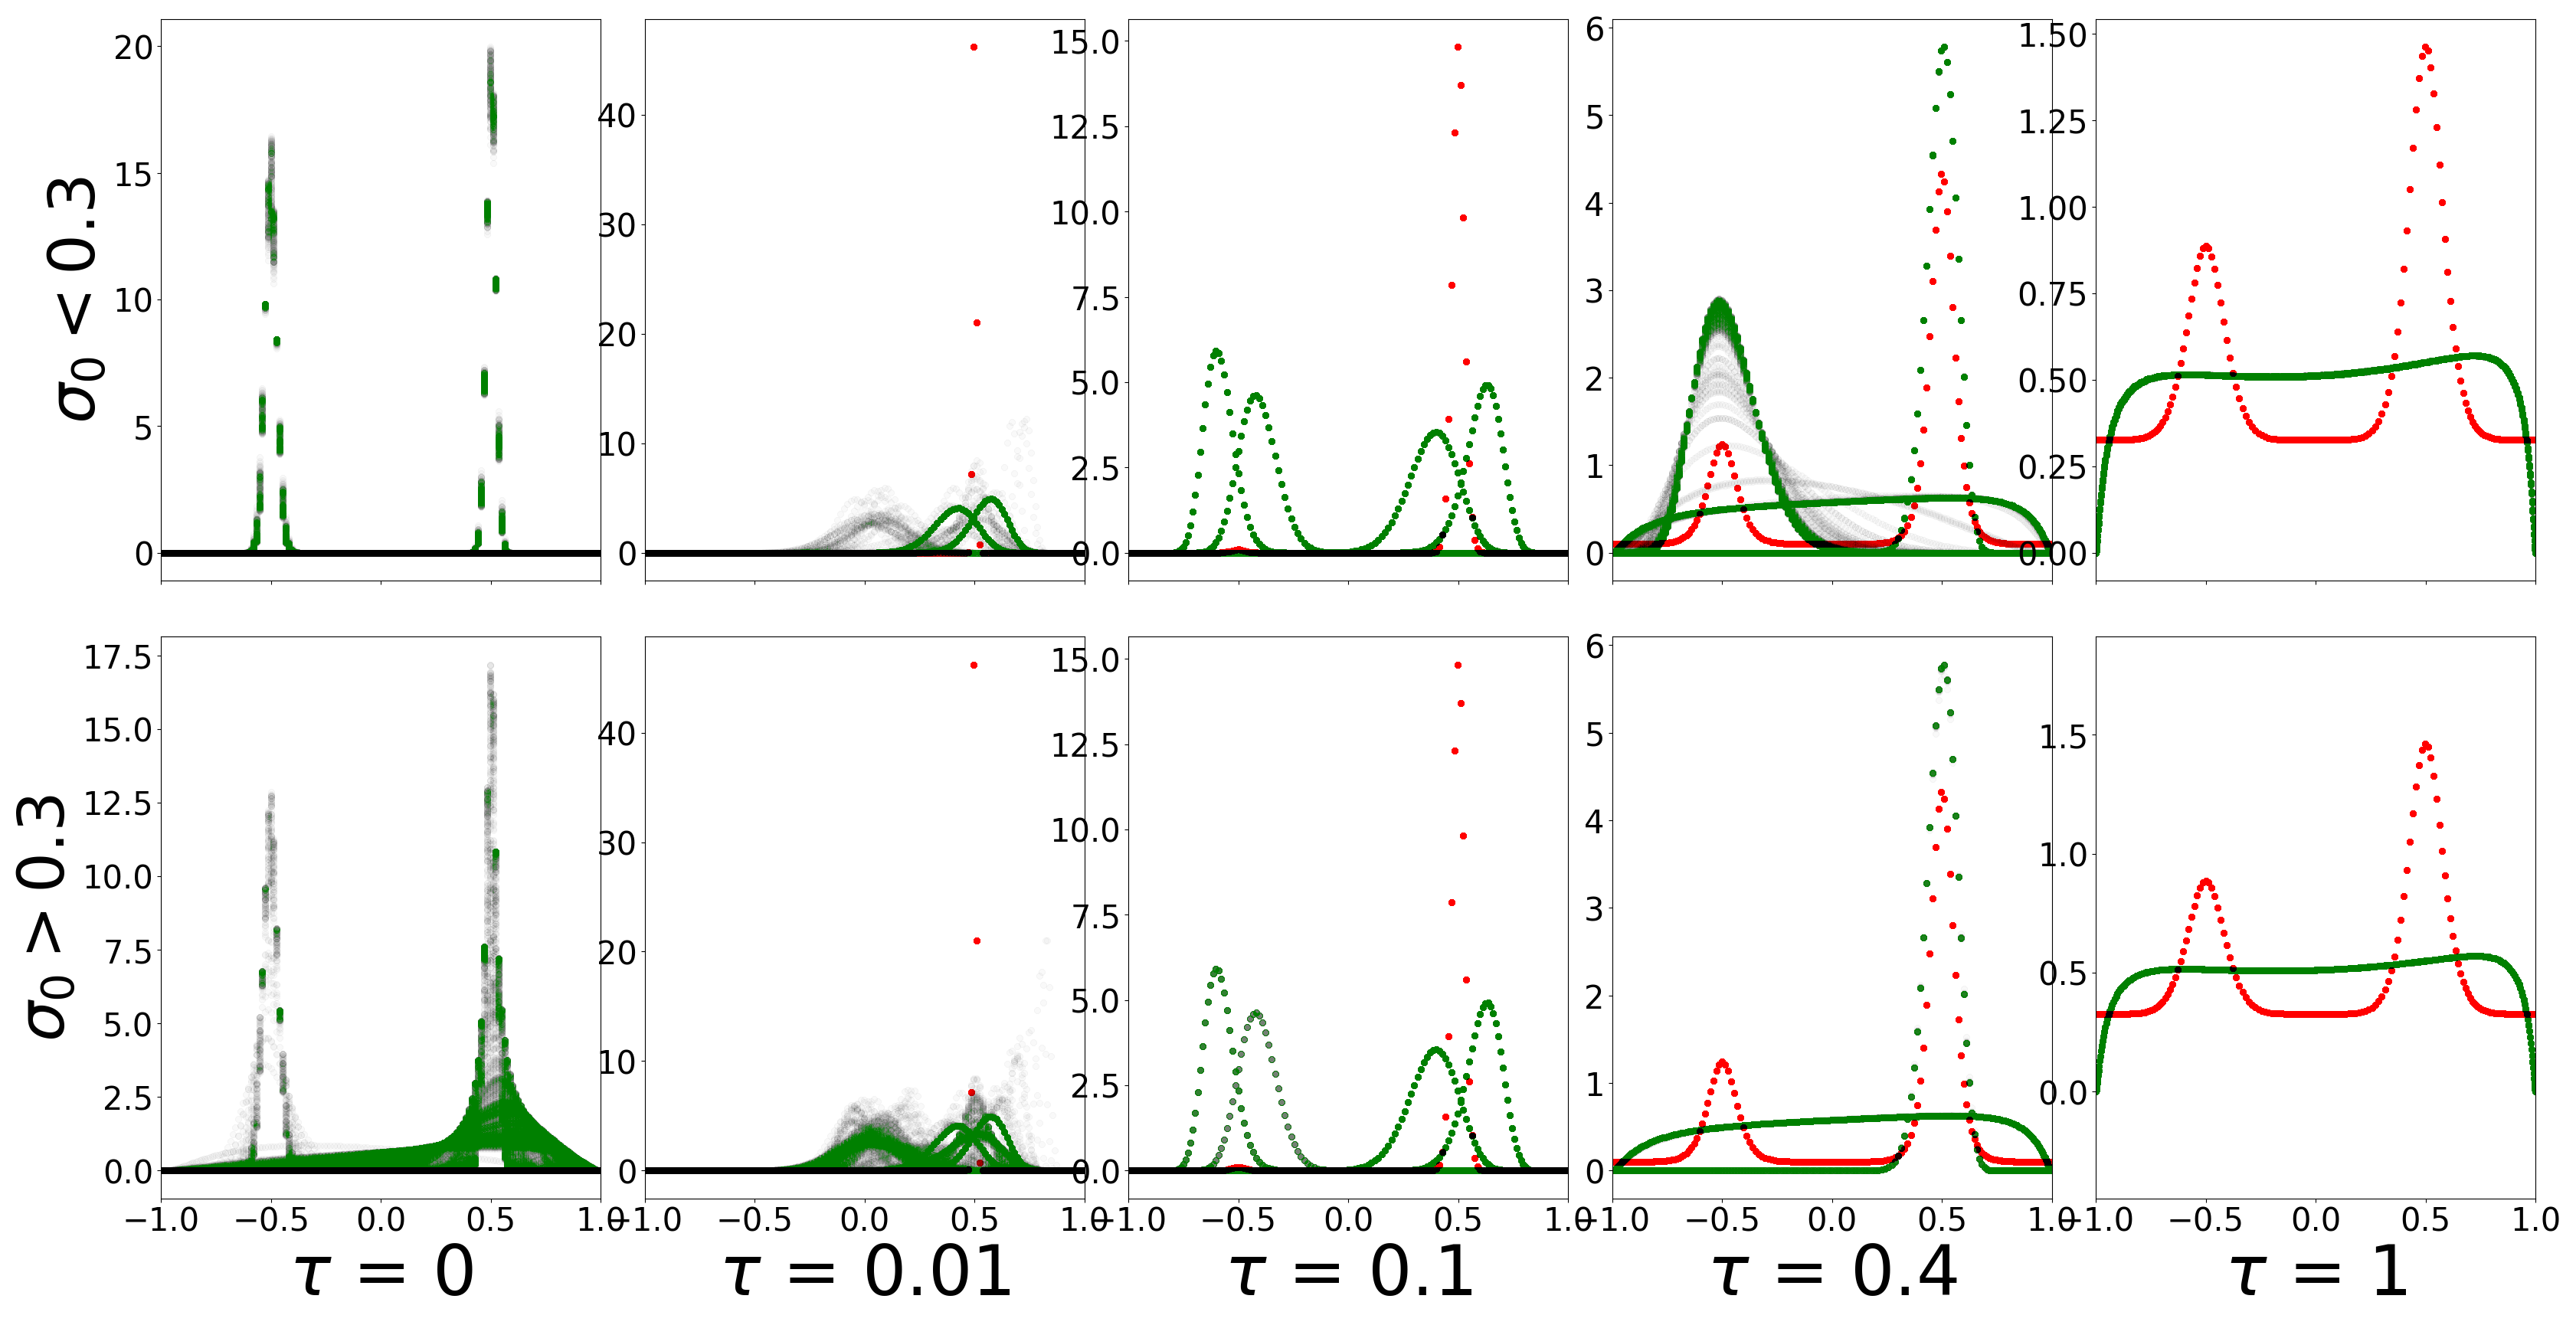
\includegraphics[width=1\columnwidth]{figs/bandit/notlearnQ/modes=1/sgd/pdf_reverse_optim=sgd_modes=1_lr=0.01.png}
    \caption{Reverse KL, SGD.}
    \label{fig:bandit-pdf-reverse-sgd}
  \end{subfigure}
  \caption{Final policy PDFs with unimodal policy. Red is the learned PDF of the policy and green is the target distribution. }
\end{figure}

\clearpage

% \textbf{Bimodal Policy}

% \begin{figure}[!ht]
%   \centering
%   \begin{subfigure}[b]{0.4\linewidth}
%     \centering
%     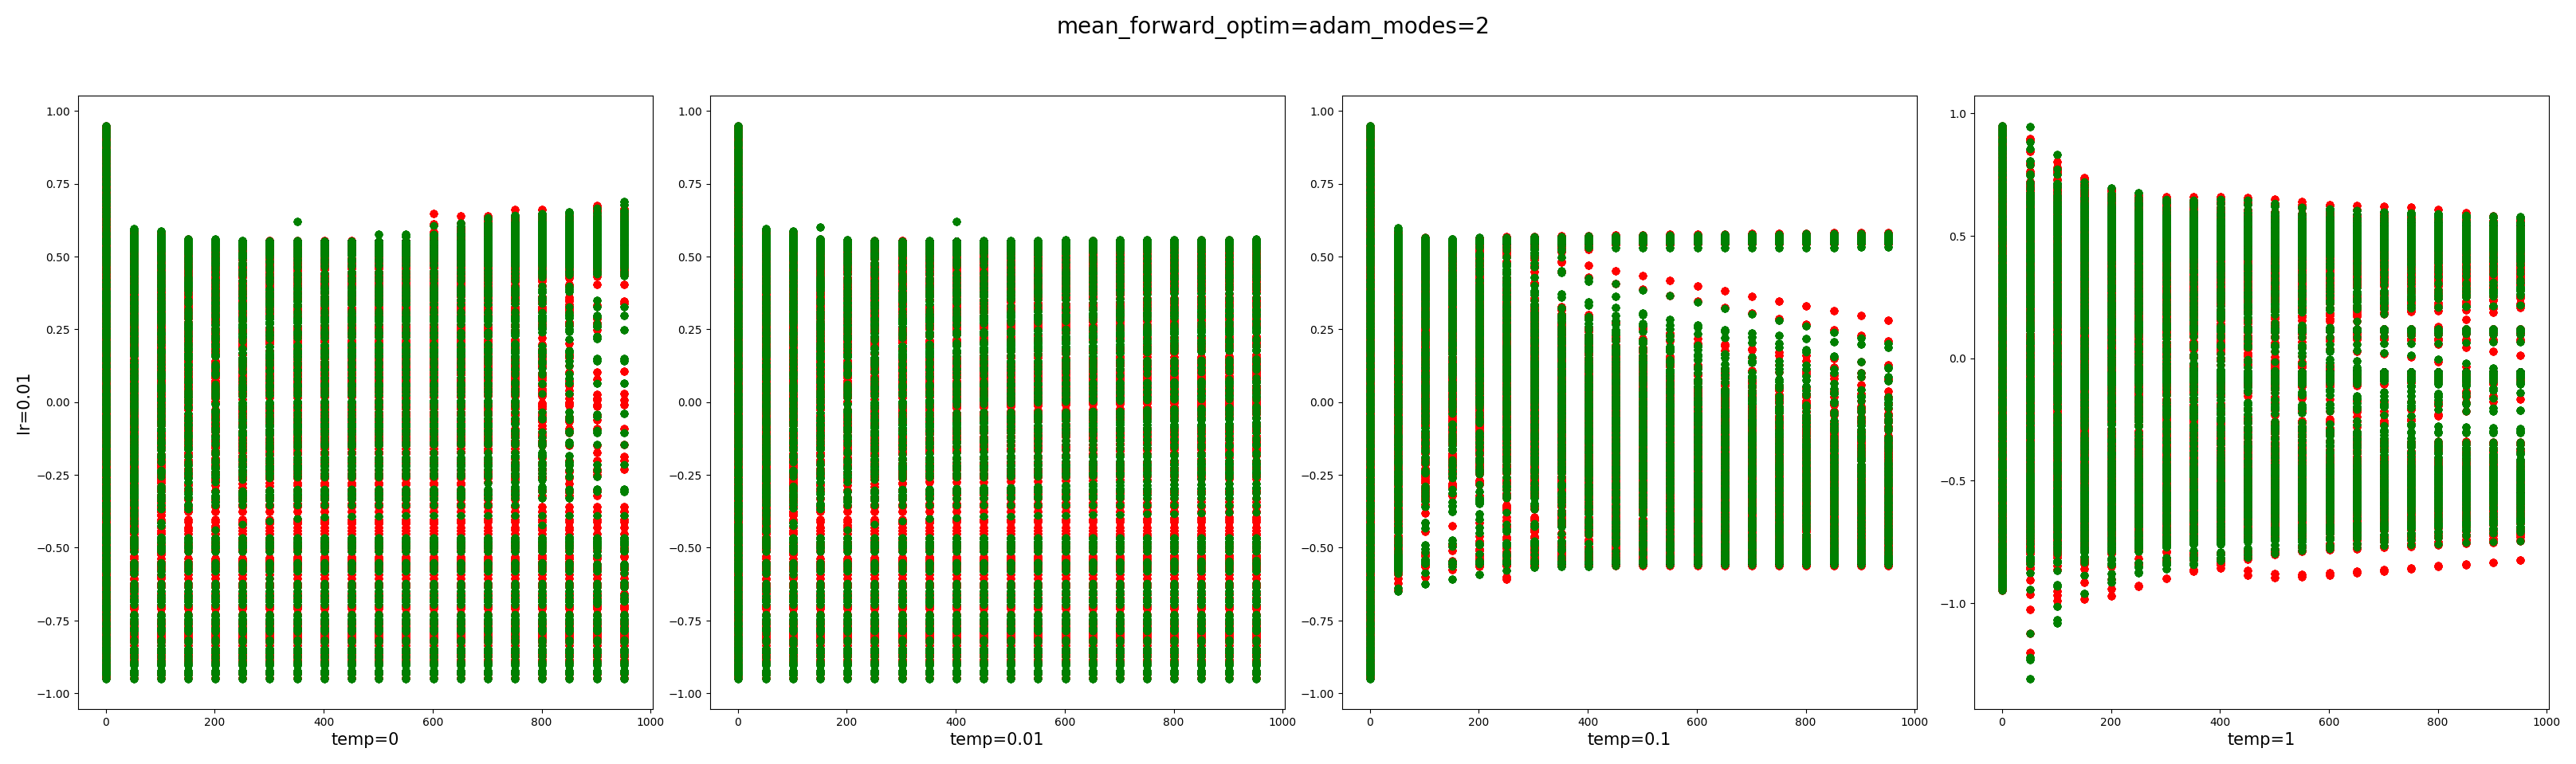
\includegraphics[width=1\columnwidth]{figs/bandit/notlearnQ/modes=2/adam/mean_forward_optim=adam_modes=2.png}
%     \caption{Forward KL, Adam.}
%     \label{fig:bandit-mean-forward-adam-bimodal}
%   \end{subfigure}%
%   \begin{subfigure}[b]{0.4\linewidth}
%     \centering
%     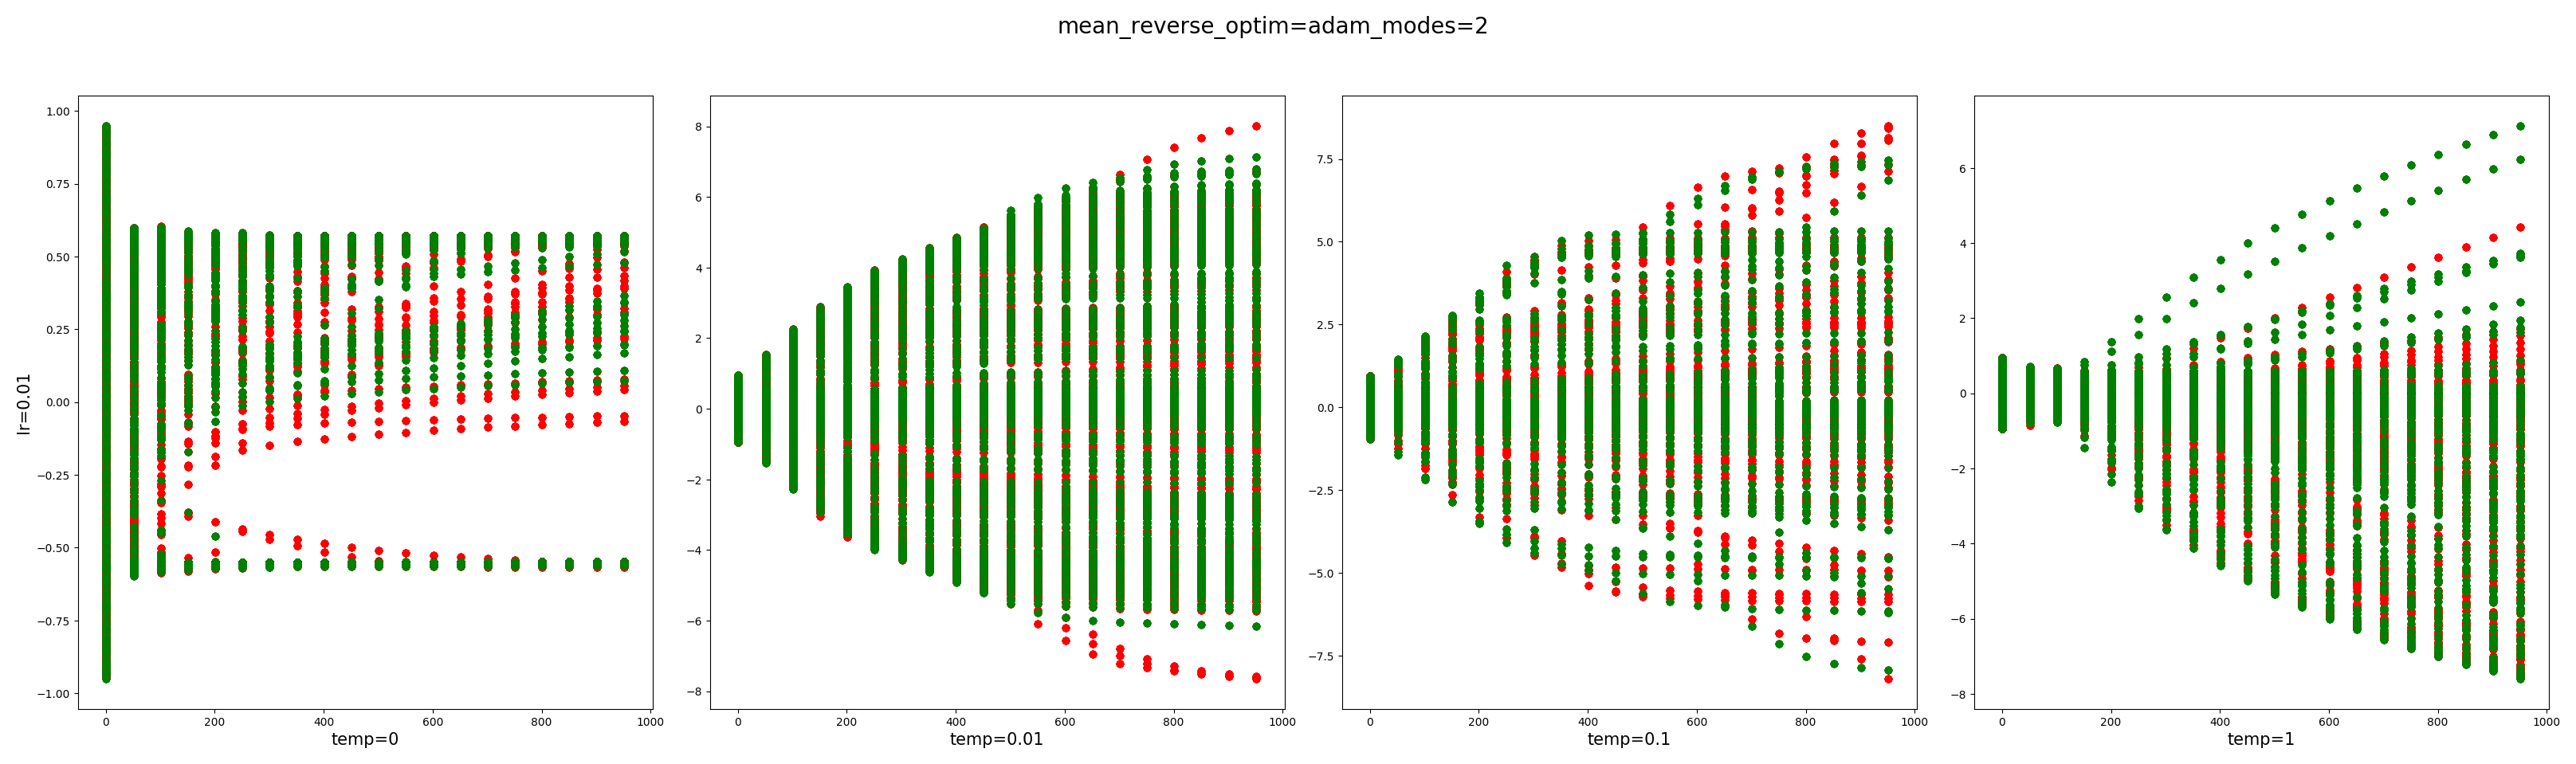
\includegraphics[width=1\columnwidth]{figs/bandit/notlearnQ/modes=2/adam/mean_reverse_optim=adam_modes=2.png}
%     \caption{Reverse KL, Adam. }
%     \label{fig:bandit-mean-reverse-adam-bimodal}
%   \end{subfigure}
  
%   \begin{subfigure}[b]{0.4\linewidth}
%     \centering
%     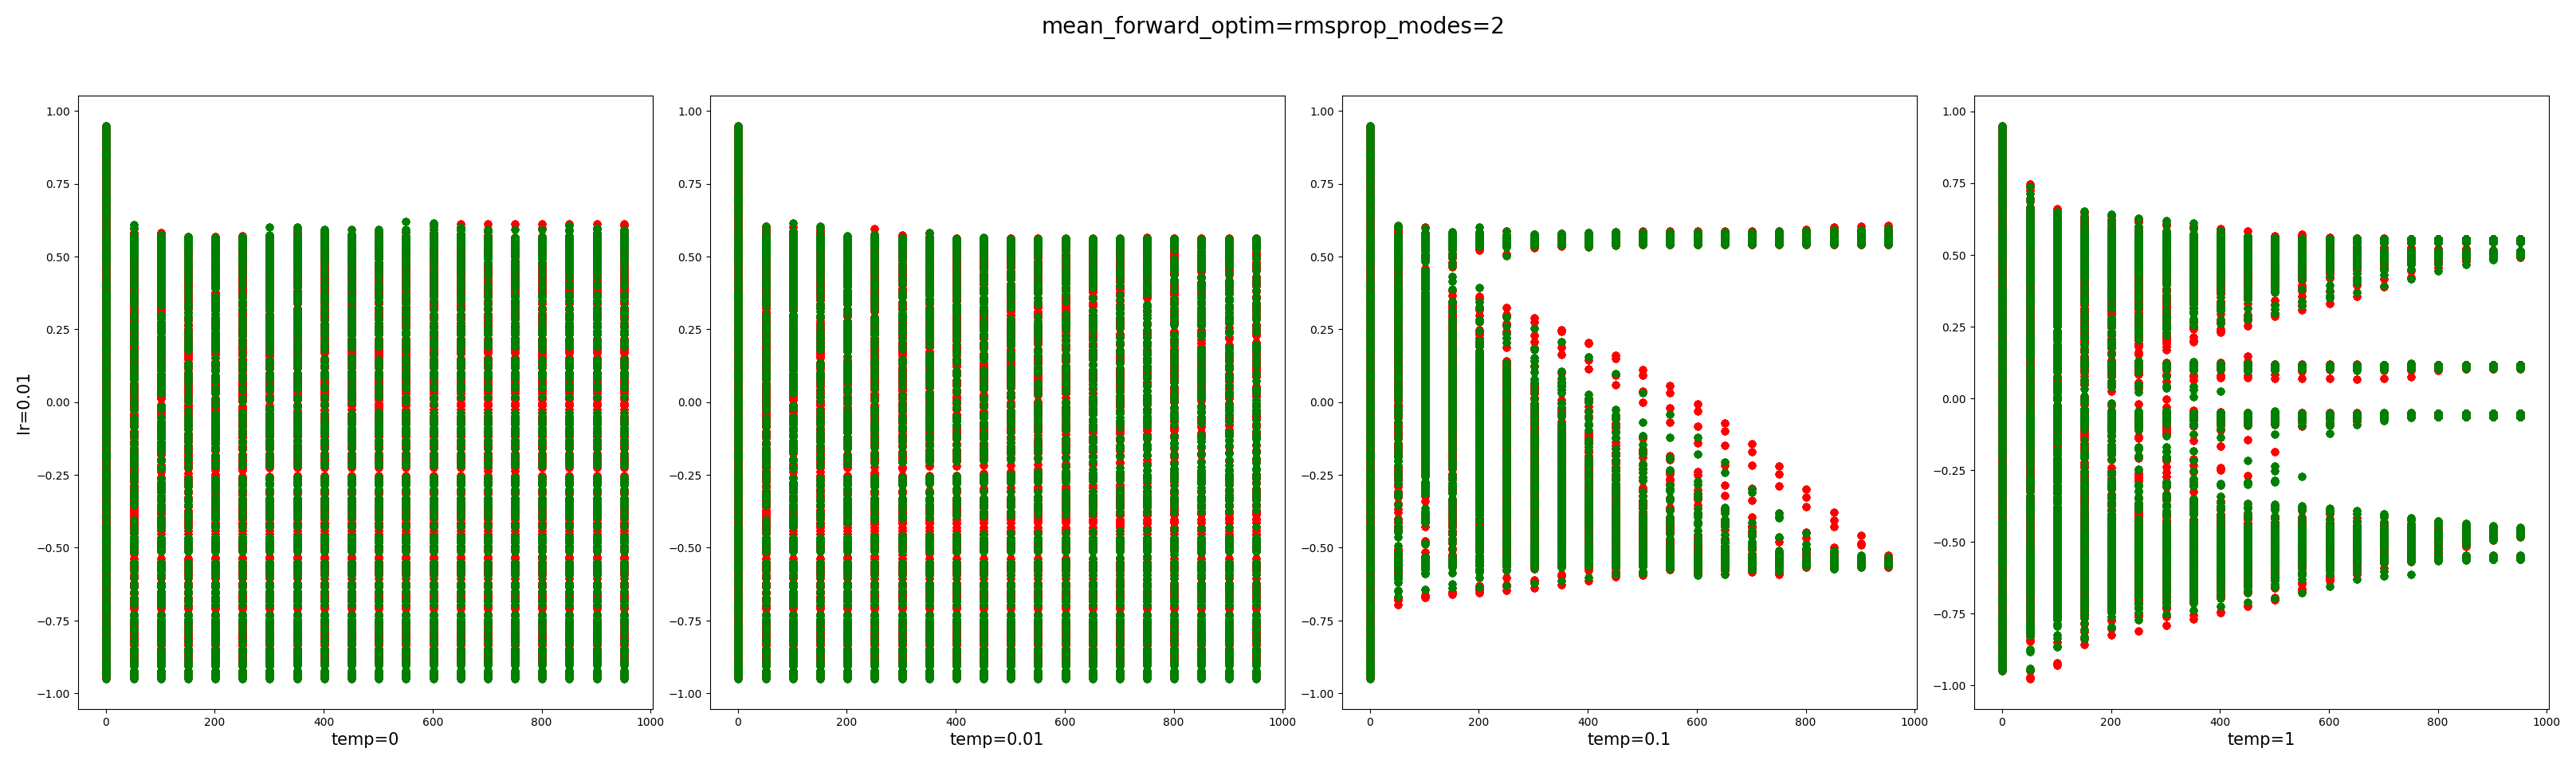
\includegraphics[width=1\columnwidth]{figs/bandit/notlearnQ/modes=2/rmsprop/mean_forward_optim=rmsprop_modes=2.png}
%     \caption{Forward KL, RMSprop.}
%     \label{fig:bandit-mean-forward-rmsprop-bimodal}
%   \end{subfigure}%
%   \begin{subfigure}[b]{0.4\linewidth}
%     \centering
%     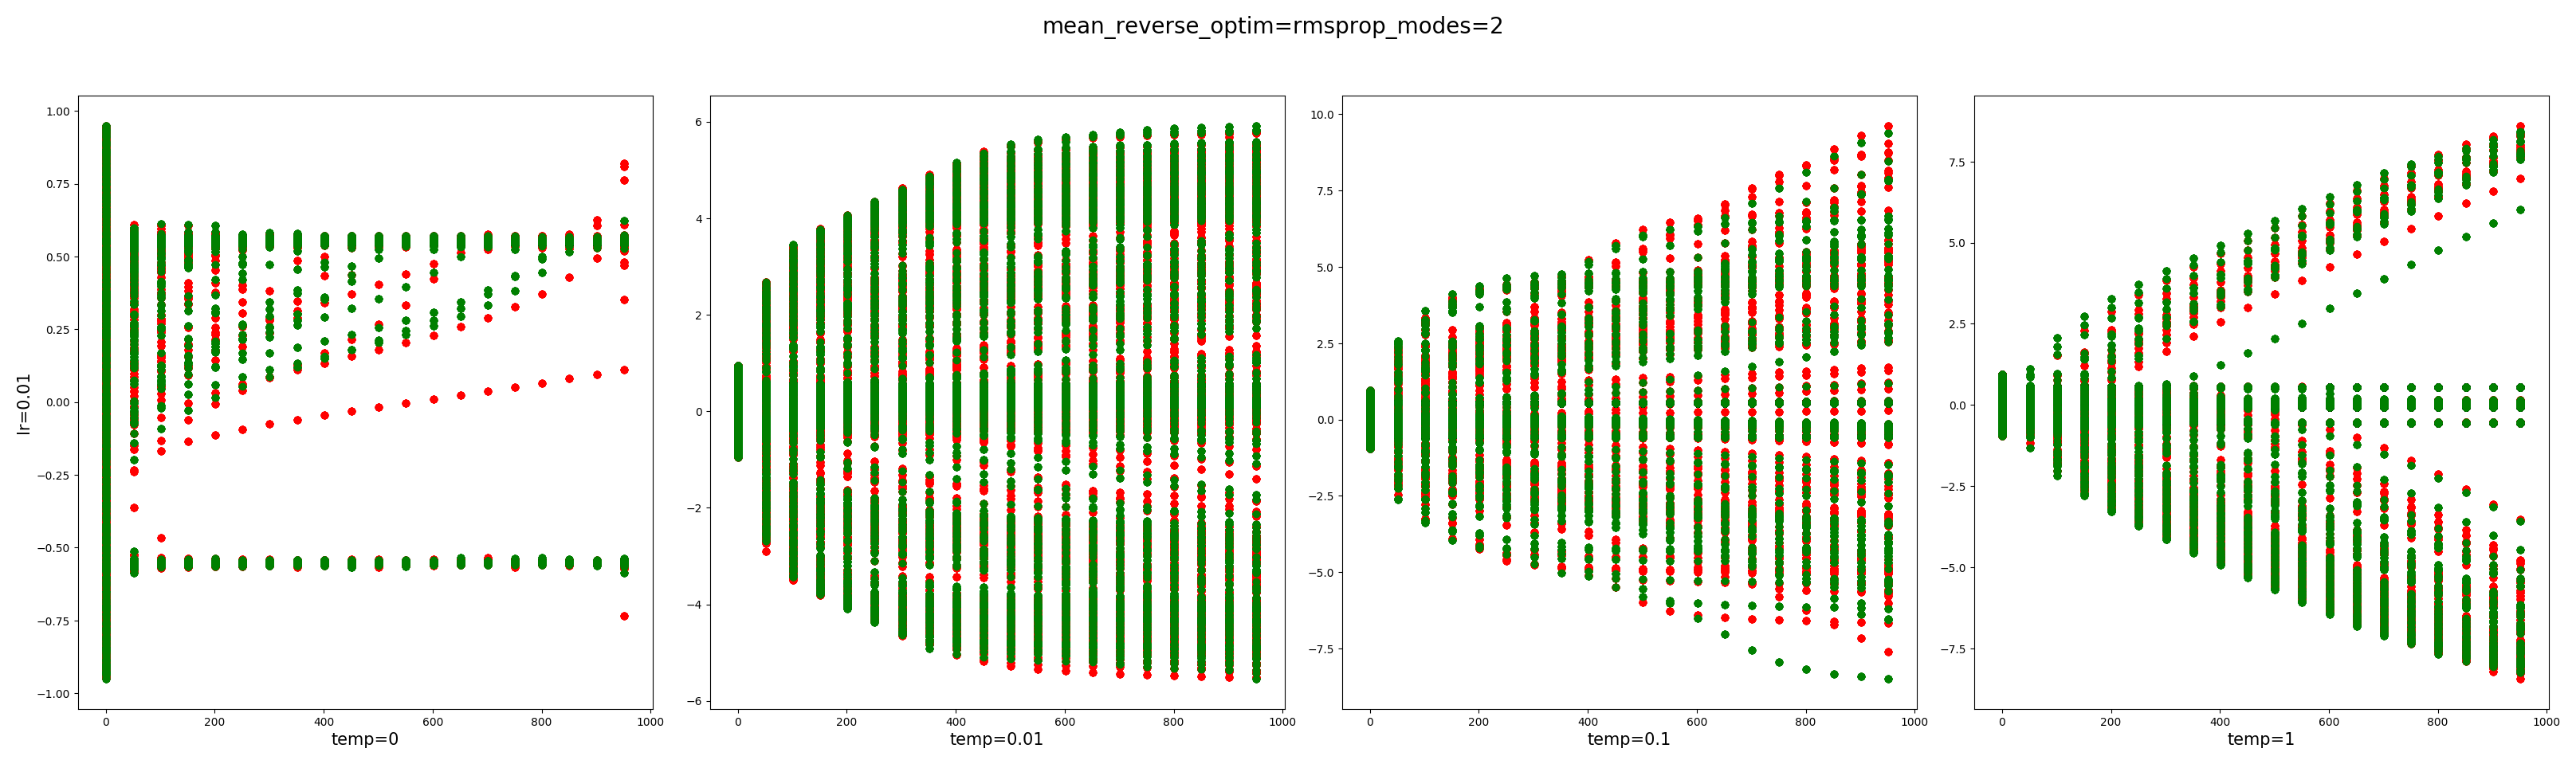
\includegraphics[width=1\columnwidth]{figs/bandit/notlearnQ/modes=2/rmsprop/mean_reverse_optim=rmsprop_modes=2.png}
%     \caption{Reverse KL, RMSprop. }
%     \label{fig:bandit-mean-reverse-rmsprop-bimodal}
%   \end{subfigure}
  
%   \begin{subfigure}[b]{0.4\linewidth}
%     \centering
%     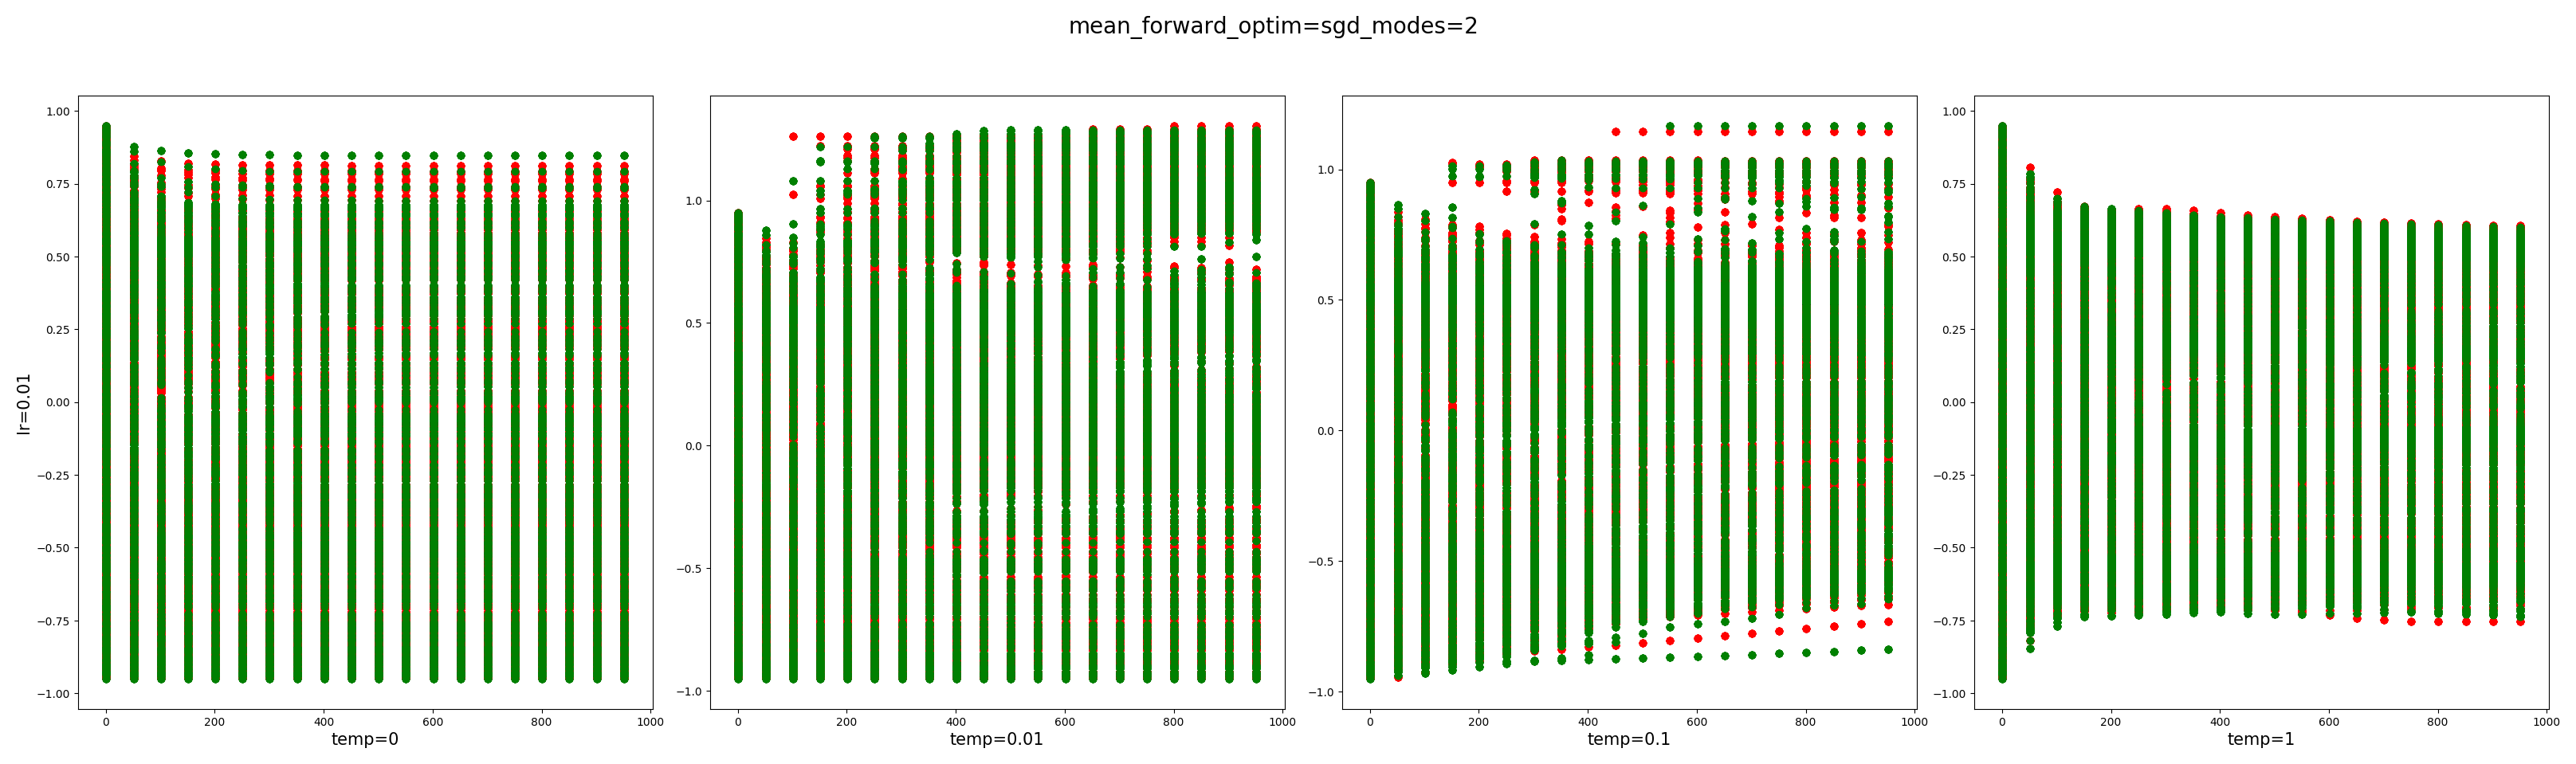
\includegraphics[width=1\columnwidth]{figs/bandit/notlearnQ/modes=2/sgd/mean_forward_optim=sgd_modes=2.png}
%     \caption{Forward KL, SGD.}
%     \label{fig:bandit-mean-forward-sgd-bimodal}
%   \end{subfigure}%
%   \begin{subfigure}[b]{0.4\linewidth}
%     \centering
%     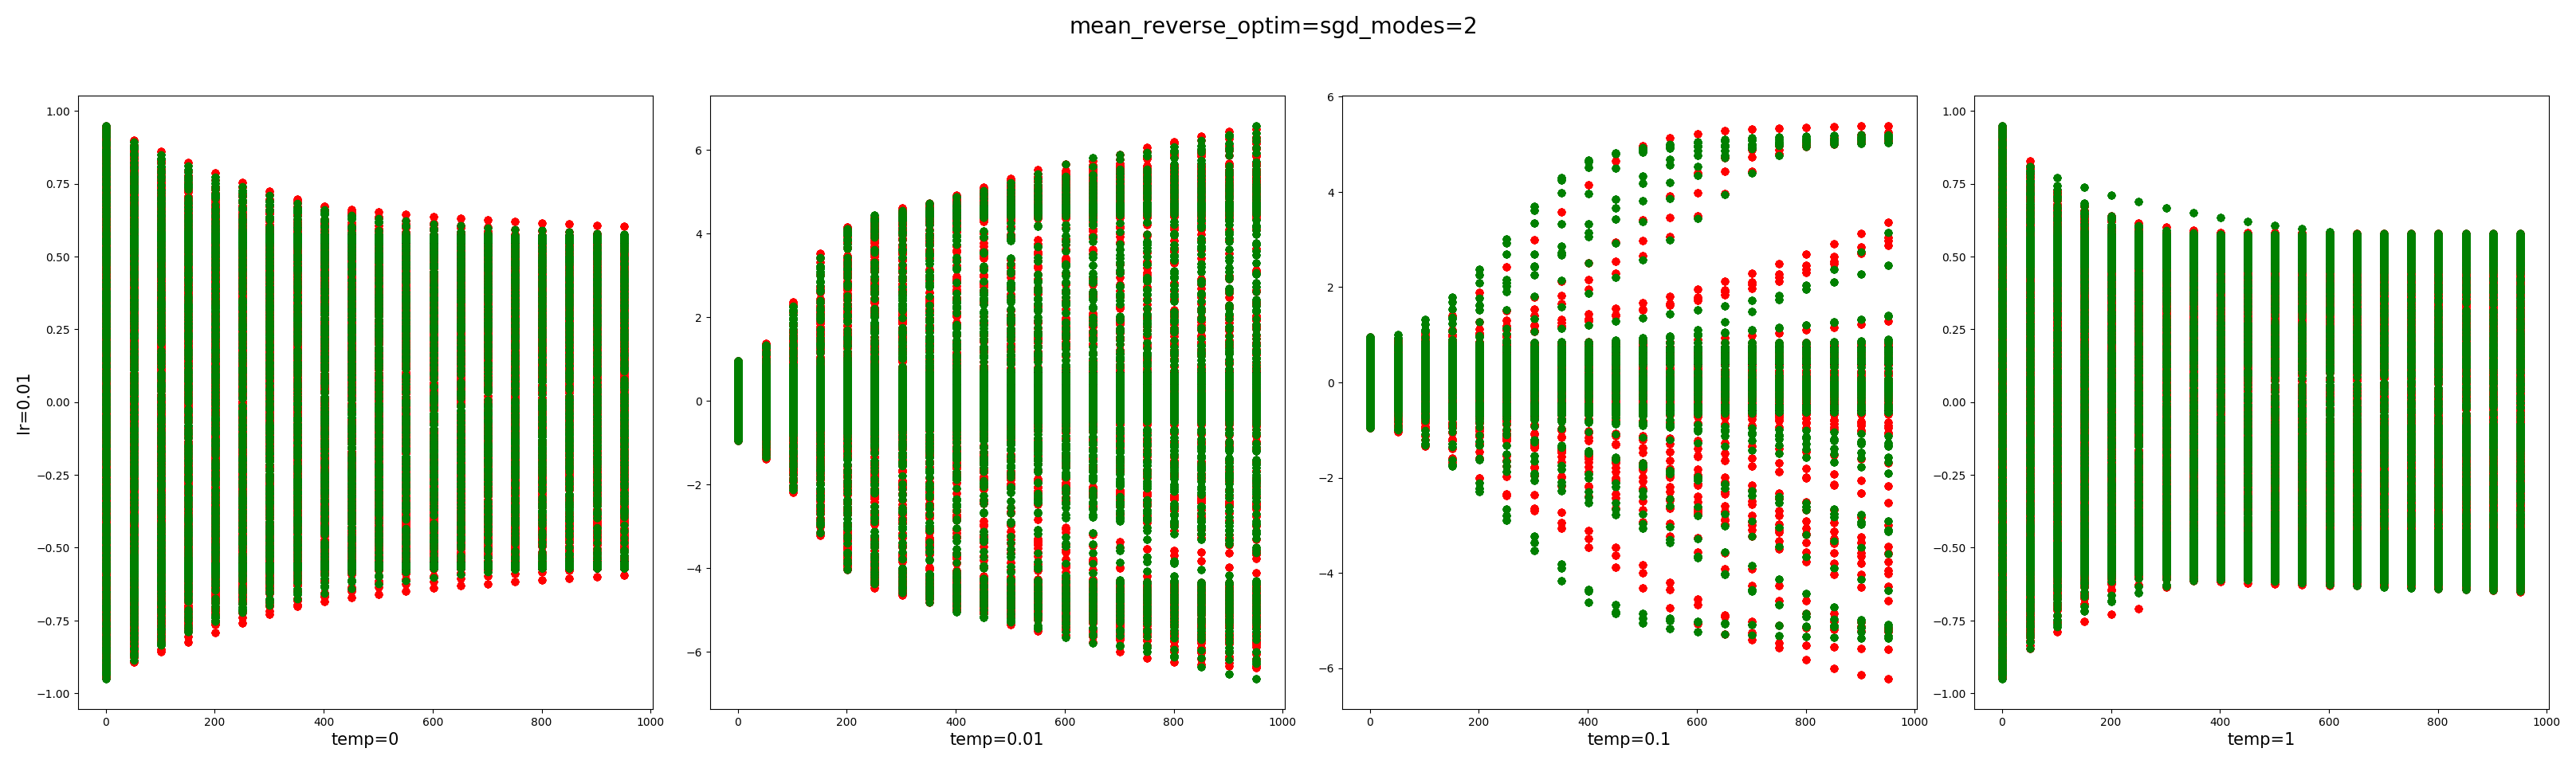
\includegraphics[width=1\columnwidth]{figs/bandit/notlearnQ/modes=2/sgd/mean_reverse_optim=sgd_modes=2.png}
%     \caption{Reverse KL, SGD.}
%     \label{fig:bandit-mean-reverse-sgd-bimodal}
%   \end{subfigure}
%   \caption{Mean over time with bimodal policy. Different colours are different modes.}
% \end{figure}


% \begin{figure}[!ht]
%   \centering
%   \begin{subfigure}[b]{0.4\linewidth}
%     \centering
%     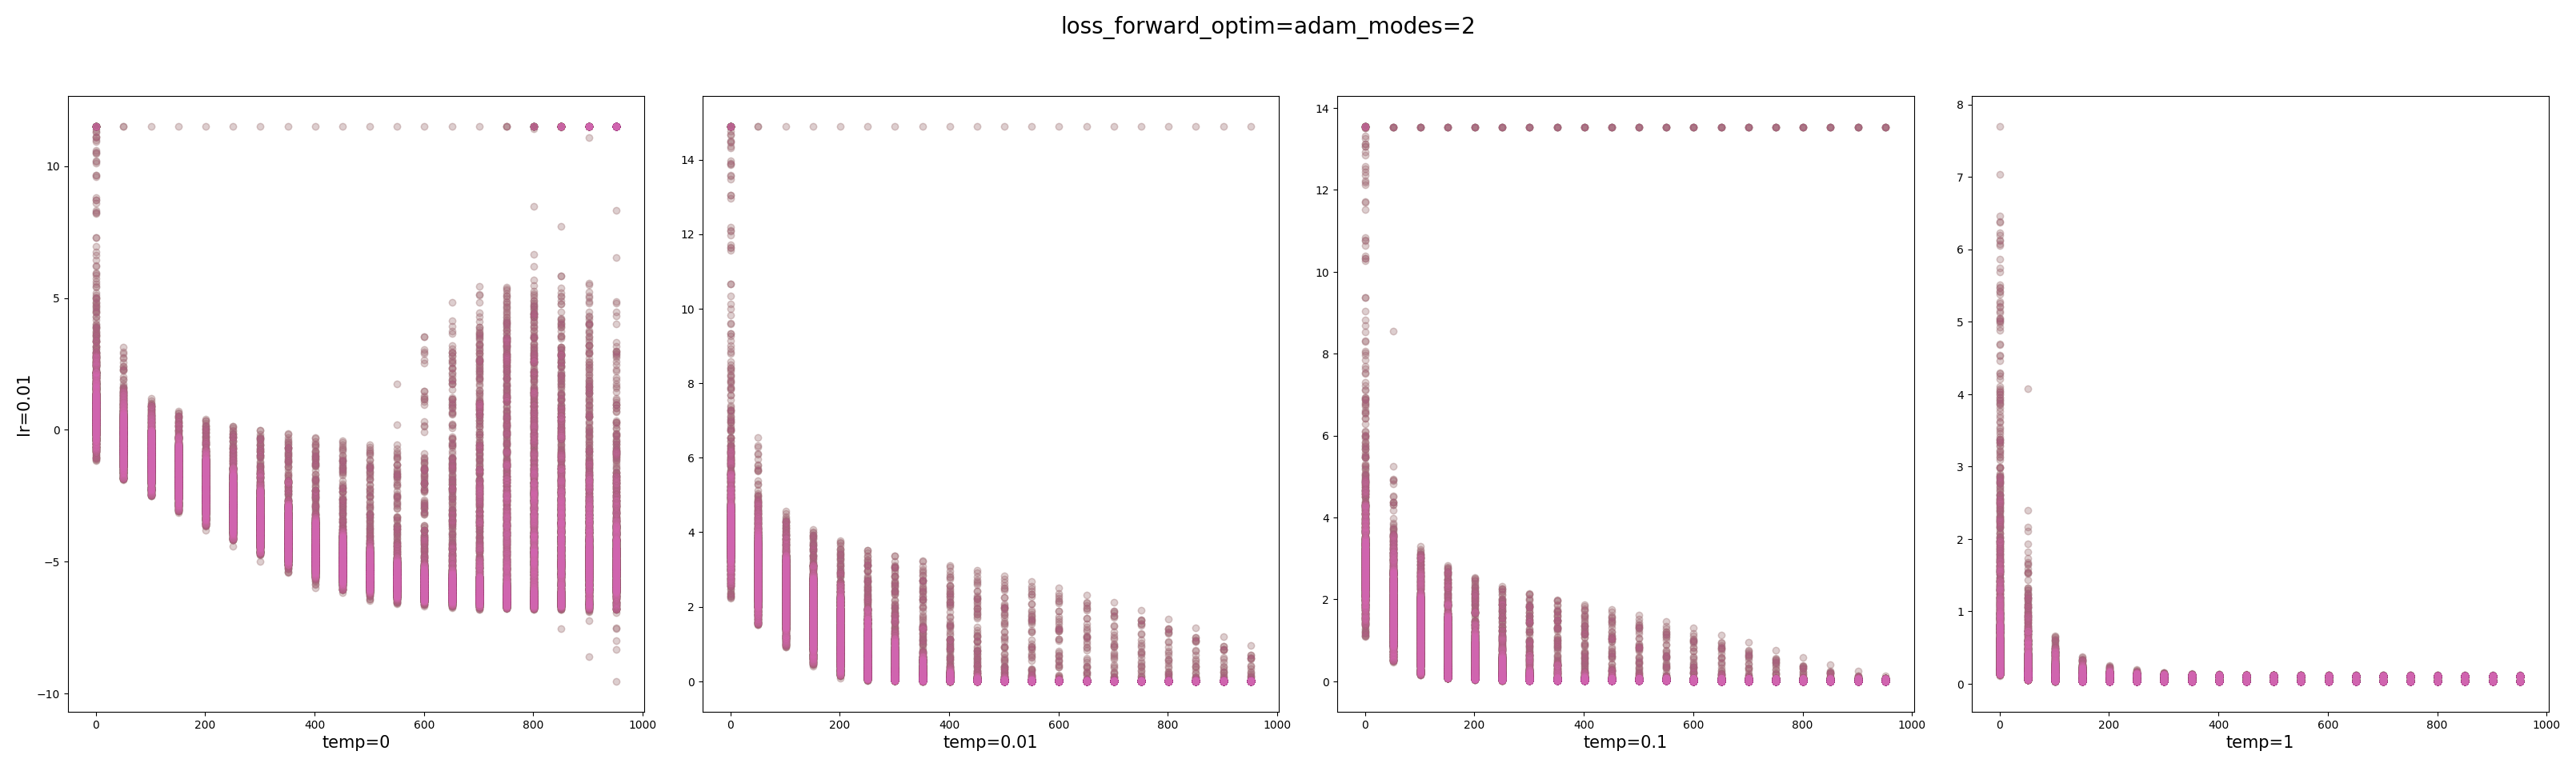
\includegraphics[width=1\columnwidth]{figs/bandit/notlearnQ/modes=2/adam/loss_forward_optim=adam_modes=2.png}
%     \caption{Forward KL, Adam.}
%     \label{fig:bandit-loss-forward-adam-bimodal}
%   \end{subfigure}%
%   \begin{subfigure}[b]{0.4\linewidth}
%     \centering
%     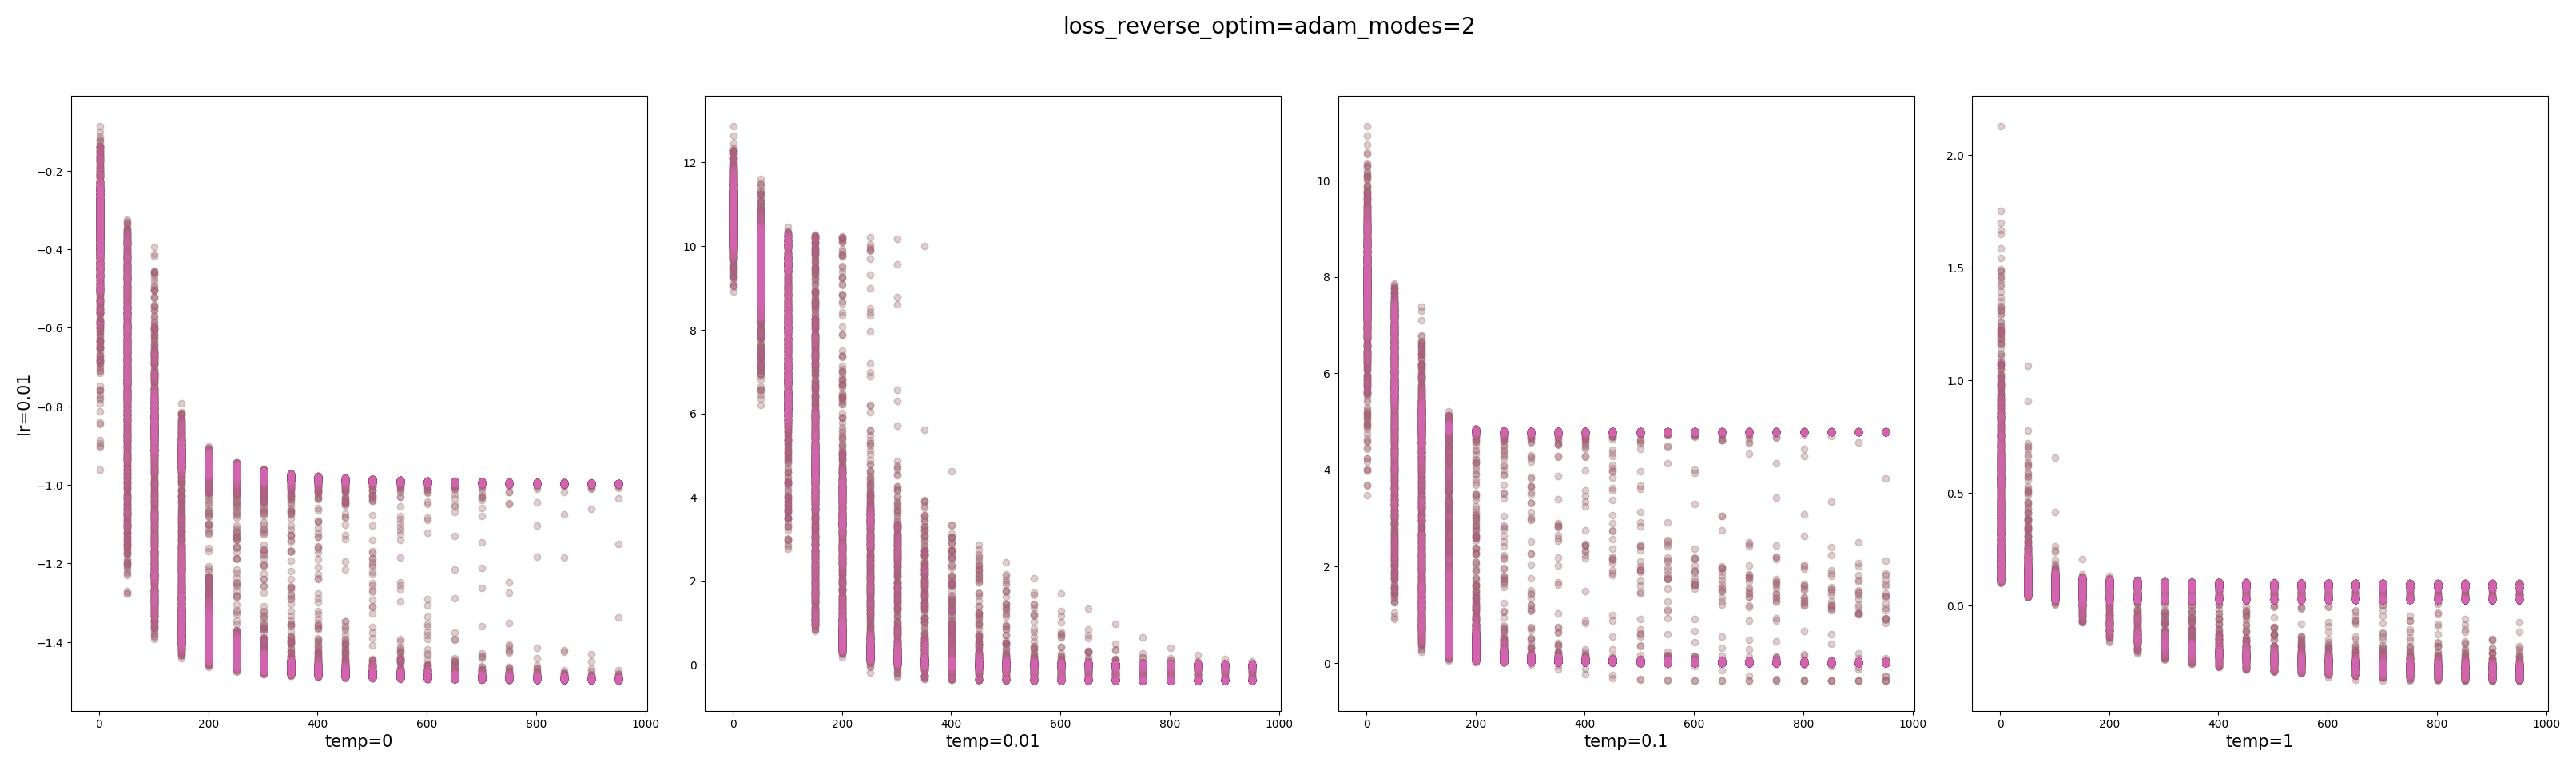
\includegraphics[width=1\columnwidth]{figs/bandit/notlearnQ/modes=2/adam/loss_reverse_optim=adam_modes=2.png}
%     \caption{Reverse KL, Adam. }
%     \label{fig:bandit-loss-reverse-adam-bimodal}
%   \end{subfigure}
  
%   \begin{subfigure}[b]{0.4\linewidth}
%     \centering
%     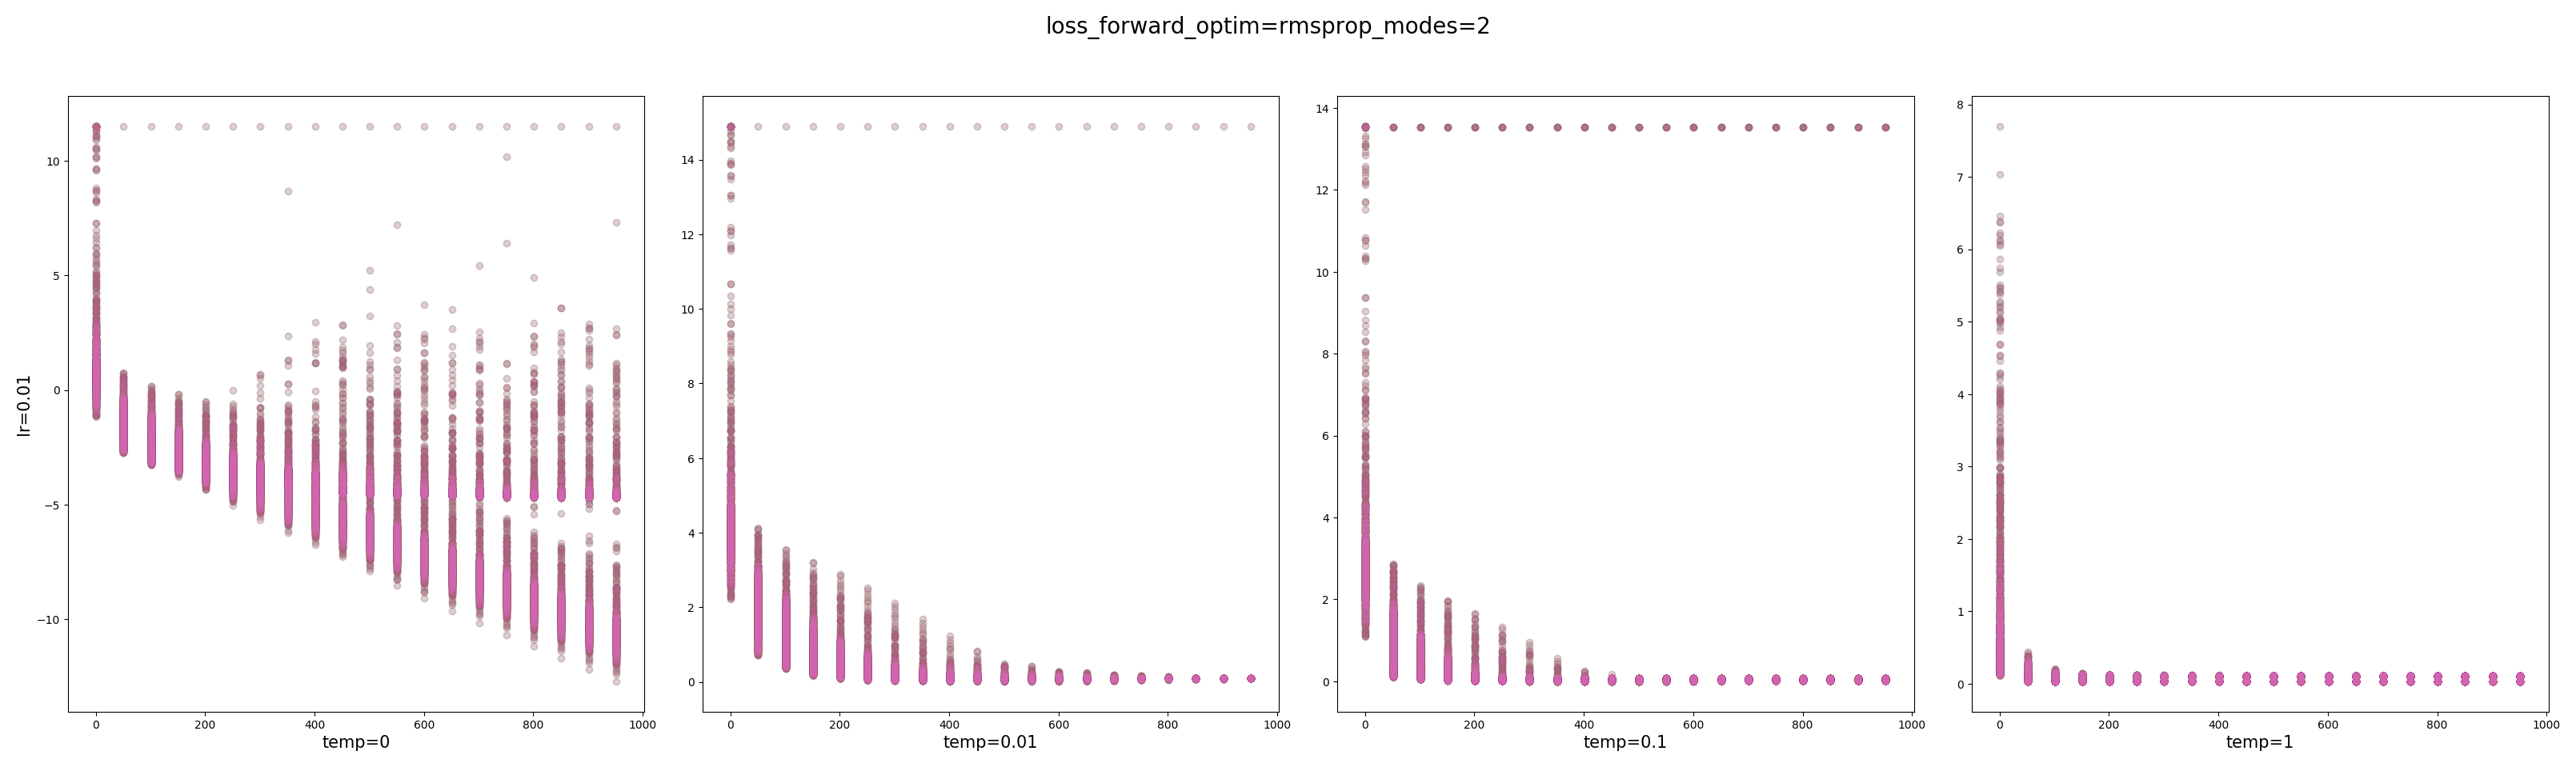
\includegraphics[width=1\columnwidth]{figs/bandit/notlearnQ/modes=2/rmsprop/loss_forward_optim=rmsprop_modes=2.png}
%     \caption{Forward KL, RMSprop.}
%     \label{fig:bandit-loss-forward-rmsprop-bimodal}
%   \end{subfigure}%
%   \begin{subfigure}[b]{0.4\linewidth}
%     \centering
%     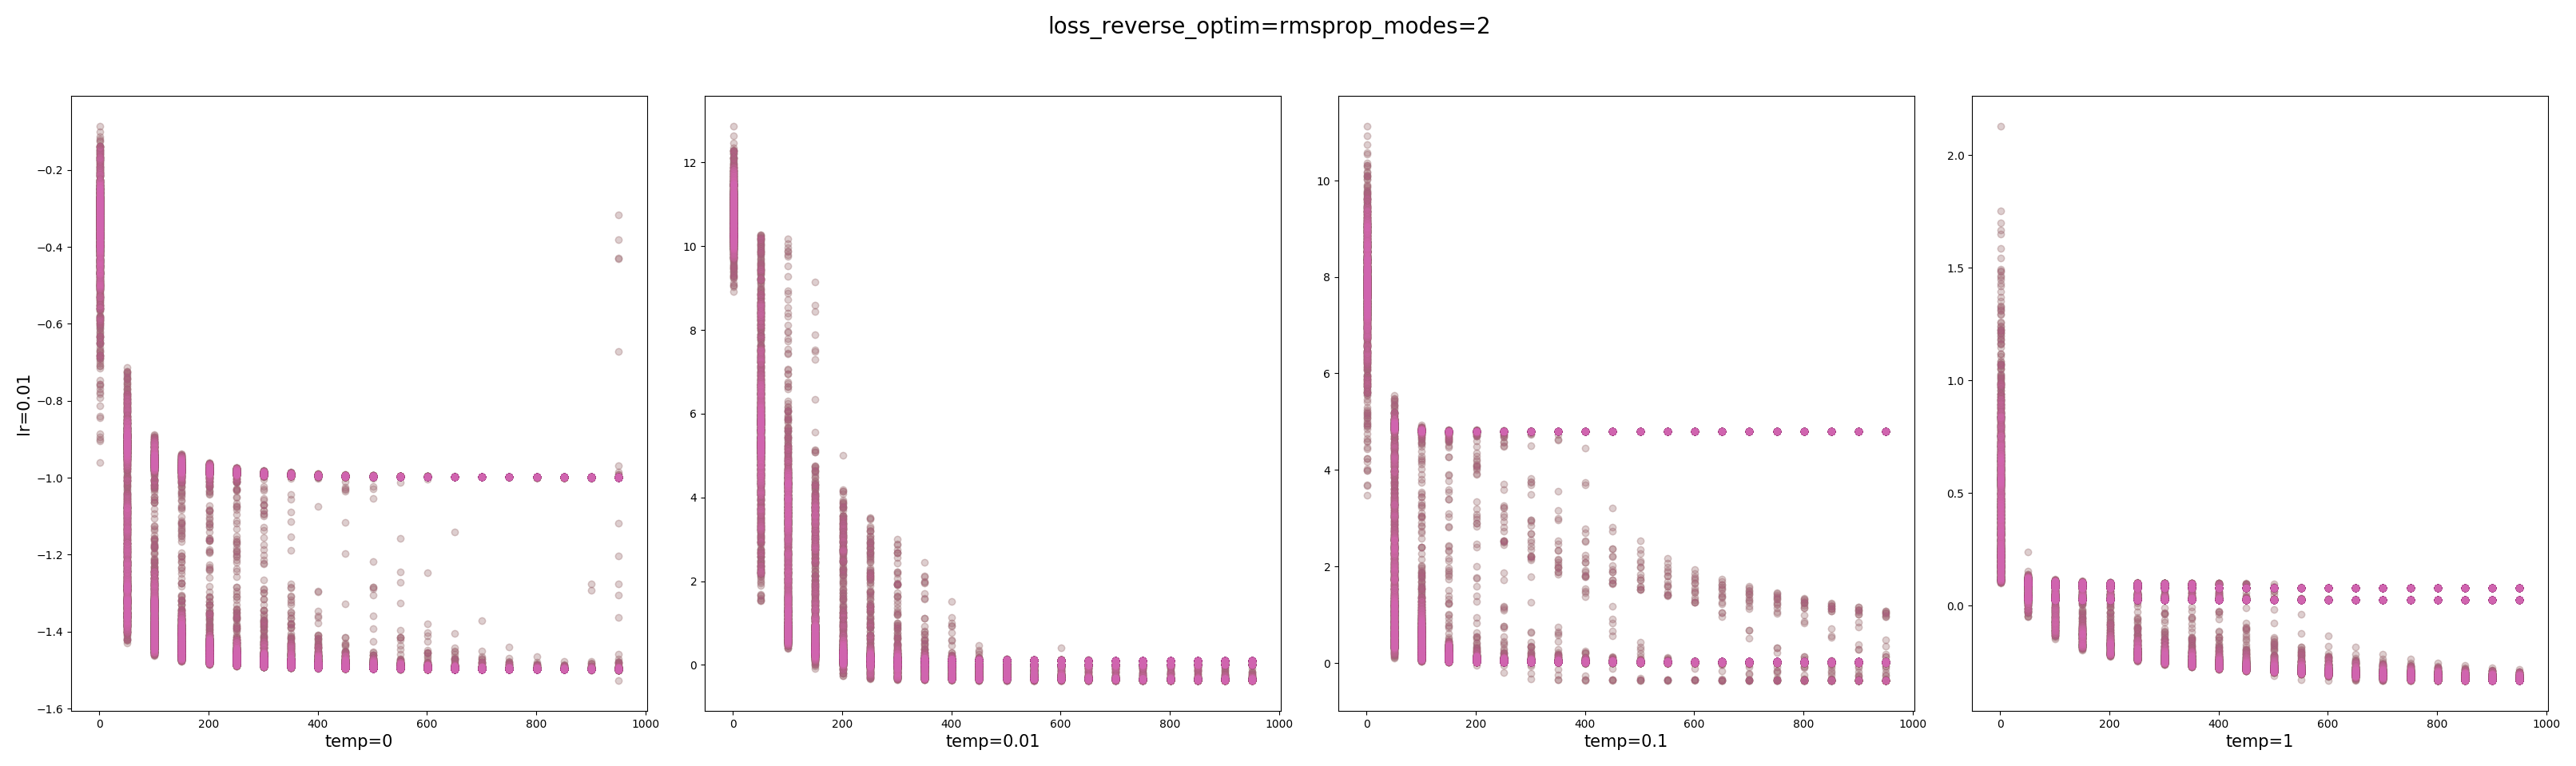
\includegraphics[width=1\columnwidth]{figs/bandit/notlearnQ/modes=2/rmsprop/loss_reverse_optim=rmsprop_modes=2.png}
%     \caption{Reverse KL, RMSprop. }
%     \label{fig:bandit-loss-reverse-rmsprop-bimodal}
%   \end{subfigure}
  
%   \begin{subfigure}[b]{0.4\linewidth}
%     \centering
%     \includegraphics[width=1\columnwidth]{figs/bandit/notlearnQ/modes=2/sgd/loss_forward_optim=sgd_modes=2.png}
%     \caption{Forward KL, SGD.}
%     \label{fig:bandit-loss-forward-sgd-bimodal}
%   \end{subfigure}%
%   \begin{subfigure}[b]{0.4\linewidth}
%     \centering
%     \includegraphics[width=1\columnwidth]{figs/bandit/notlearnQ/modes=2/sgd/loss_reverse_optim=sgd_modes=2.png}
%     \caption{Reverse KL, SGD.}
%     \label{fig:bandit-loss-reverse-sgd-bimodal}
%   \end{subfigure}
%   \caption{Loss over time with bimodal policy. Different colours are different modes.}
% \end{figure}


% \begin{figure}[!ht]
%   \centering
%   \begin{subfigure}[b]{0.4\linewidth}
%     \centering
%     \includegraphics[width=1\columnwidth]{figs/bandit/notlearnQ/modes=2/adam/std_forward_optim=adam_modes=2.png}
%     \caption{Forward KL, Adam.}
%     \label{fig:bandit-std-forward-adam-bimodal}
%   \end{subfigure}%
%   \begin{subfigure}[b]{0.4\linewidth}
%     \centering
%     \includegraphics[width=1\columnwidth]{figs/bandit/notlearnQ/modes=2/adam/std_reverse_optim=adam_modes=2.png}
%     \caption{Reverse KL, Adam. }
%     \label{fig:bandit-std-reverse-adam-bimodal}
%   \end{subfigure}
  
%   \begin{subfigure}[b]{0.4\linewidth}
%     \centering
%     \includegraphics[width=1\columnwidth]{figs/bandit/notlearnQ/modes=2/rmsprop/std_forward_optim=rmsprop_modes=2.png}
%     \caption{Forward KL, RMSprop.}
%     \label{fig:bandit-std-forward-rmsprop-bimodal}
%   \end{subfigure}%
%   \begin{subfigure}[b]{0.4\linewidth}
%     \centering
%     \includegraphics[width=1\columnwidth]{figs/bandit/notlearnQ/modes=2/rmsprop/std_reverse_optim=rmsprop_modes=2.png}
%     \caption{Reverse KL, RMSprop. }
%     \label{fig:bandit-std-reverse-rmsprop-bimodal}
%   \end{subfigure}
  
%   \begin{subfigure}[b]{0.4\linewidth}
%     \centering
%     \includegraphics[width=1\columnwidth]{figs/bandit/notlearnQ/modes=2/sgd/std_forward_optim=sgd_modes=2.png}
%     \caption{Forward KL, SGD.}
%     \label{fig:bandit-std-forward-sgd-bimodal}
%   \end{subfigure}%
%   \begin{subfigure}[b]{0.4\linewidth}
%     \centering
%     \includegraphics[width=1\columnwidth]{figs/bandit/notlearnQ/modes=2/sgd/std_reverse_optim=sgd_modes=2.png}
%     \caption{Reverse KL, SGD.}
%     \label{fig:bandit-std-reverse-sgd-bimodal}
%   \end{subfigure}
%   \caption{Standard deviation over time with bimodal policy. Different colours are different modes.}
% \end{figure}

% \begin{figure}[!ht]
%   \centering
%   \begin{subfigure}[b]{0.4\linewidth}
%     \centering
%     \includegraphics[width=1\columnwidth]{figs/bandit/notlearnQ/modes=2/adam/pdf_forward_optim=adam_modes=2.png}
%     \caption{Forward KL, Adam.}
%     \label{fig:bandit-pdf-forward-adam-bimodal}
%   \end{subfigure}%
%   \begin{subfigure}[b]{0.4\linewidth}
%     \centering
%     \includegraphics[width=1\columnwidth]{figs/bandit/notlearnQ/modes=2/adam/pdf_reverse_optim=adam_modes=2.png}
%     \caption{Reverse KL, Adam. }
%     \label{fig:bandit-pdf-reverse-adam-bimodal}
%   \end{subfigure}
  
%   \begin{subfigure}[b]{0.4\linewidth}
%     \centering
%     \includegraphics[width=1\columnwidth]{figs/bandit/notlearnQ/modes=2/rmsprop/pdf_forward_optim=rmsprop_modes=2.png}
%     \caption{Forward KL, RMSprop.}
%     \label{fig:bandit-pdf-forward-rmsprop-bimodal}
%   \end{subfigure}%
%   \begin{subfigure}[b]{0.4\linewidth}
%     \centering
%     \includegraphics[width=1\columnwidth]{figs/bandit/notlearnQ/modes=2/rmsprop/pdf_reverse_optim=rmsprop_modes=2.png}
%     \caption{Reverse KL, RMSprop. }
%     \label{fig:bandit-pdf-reverse-rmsprop-bimodal}
%   \end{subfigure}
  
%   \begin{subfigure}[b]{0.4\linewidth}
%     \centering
%     \includegraphics[width=1\columnwidth]{figs/bandit/notlearnQ/modes=2/sgd/pdf_forward_optim=sgd_modes=2.png}
%     \caption{Forward KL, SGD.}
%     \label{fig:bandit-pdf-forward-sgd-bimodal}
%   \end{subfigure}%
%   \begin{subfigure}[b]{0.4\linewidth}
%     \centering
%     \includegraphics[width=1\columnwidth]{figs/bandit/notlearnQ/modes=2/sgd/pdf_reverse_optim=sgd_modes=2.png}
%     \caption{Reverse KL, SGD.}
%     \label{fig:bandit-pdf-reverse-sgd-bimodal}
%   \end{subfigure}
%   \caption{Final policy PDFs with bimodal policy. Green is learned policy and red is target policy.}
% \end{figure}


% \clearpage
% \textbf{Trimodal Policy}

% \begin{figure}[!ht]
%   \centering
%   \begin{subfigure}[b]{0.4\linewidth}
%     \centering
%     \includegraphics[width=1\columnwidth]{figs/bandit/notlearnQ/modes=3/adam/mean_forward_optim=adam_modes=3.png}
%     \caption{Forward KL, Adam.}
%     \label{fig:bandit-mean-forward-adam-trimodal}
%   \end{subfigure}%
%   \begin{subfigure}[b]{0.4\linewidth}
%     \centering
%     \includegraphics[width=1\columnwidth]{figs/bandit/notlearnQ/modes=3/adam/mean_reverse_optim=adam_modes=3.png}
%     \caption{Reverse KL, Adam. }
%     \label{fig:bandit-mean-reverse-adam-trimodal}
%   \end{subfigure}
  
%   \begin{subfigure}[b]{0.4\linewidth}
%     \centering
%     \includegraphics[width=1\columnwidth]{figs/bandit/notlearnQ/modes=3/rmsprop/mean_forward_optim=rmsprop_modes=3.png}
%     \caption{Forward KL, RMSprop.}
%     \label{fig:bandit-mean-forward-rmsprop-trimodal}
%   \end{subfigure}%
%   \begin{subfigure}[b]{0.4\linewidth}
%     \centering
%     \includegraphics[width=1\columnwidth]{figs/bandit/notlearnQ/modes=3/rmsprop/mean_reverse_optim=rmsprop_modes=3.png}
%     \caption{Reverse KL, RMSprop. }
%     \label{fig:bandit-mean-reverse-rmsprop-trimodal}
%   \end{subfigure}
  
%   \begin{subfigure}[b]{0.4\linewidth}
%     \centering
%     \includegraphics[width=1\columnwidth]{figs/bandit/notlearnQ/modes=3/sgd/mean_forward_optim=sgd_modes=3.png}
%     \caption{Forward KL, SGD.}
%     \label{fig:bandit-mean-forward-sgd-trimodal}
%   \end{subfigure}%
%   \begin{subfigure}[b]{0.4\linewidth}
%     \centering
%     \includegraphics[width=1\columnwidth]{figs/bandit/notlearnQ/modes=3/sgd/mean_reverse_optim=sgd_modes=3.png}
%     \caption{Reverse KL, SGD.}
%     \label{fig:bandit-mean-reverse-sgd-trimodal}
%   \end{subfigure}
%   \caption{Mean over time with trimodal policy. Different colours are different modes.}
% \end{figure}


% \begin{figure}[!ht]
%   \centering
%   \begin{subfigure}[b]{0.4\linewidth}
%     \centering
%     \includegraphics[width=1\columnwidth]{figs/bandit/notlearnQ/modes=3/adam/loss_forward_optim=adam_modes=3.png}
%     \caption{Forward KL, Adam.}
%     \label{fig:bandit-loss-forward-adam-trimodal}
%   \end{subfigure}%
%   \begin{subfigure}[b]{0.4\linewidth}
%     \centering
%     \includegraphics[width=1\columnwidth]{figs/bandit/notlearnQ/modes=3/adam/loss_reverse_optim=adam_modes=3.png}
%     \caption{Reverse KL, Adam. }
%     \label{fig:bandit-loss-reverse-adam-trimodal}
%   \end{subfigure}
  
%   \begin{subfigure}[b]{0.4\linewidth}
%     \centering
%     \includegraphics[width=1\columnwidth]{figs/bandit/notlearnQ/modes=3/rmsprop/loss_forward_optim=rmsprop_modes=3.png}
%     \caption{Forward KL, RMSprop.}
%     \label{fig:bandit-loss-forward-rmsprop-trimodal}
%   \end{subfigure}%
%   \begin{subfigure}[b]{0.4\linewidth}
%     \centering
%     \includegraphics[width=1\columnwidth]{figs/bandit/notlearnQ/modes=3/rmsprop/loss_reverse_optim=rmsprop_modes=3.png}
%     \caption{Reverse KL, RMSprop. }
%     \label{fig:bandit-loss-reverse-rmsprop-trimodal}
%   \end{subfigure}
  
%   \begin{subfigure}[b]{0.4\linewidth}
%     \centering
%     \includegraphics[width=1\columnwidth]{figs/bandit/notlearnQ/modes=3/sgd/loss_forward_optim=sgd_modes=3.png}
%     \caption{Forward KL, SGD.}
%     \label{fig:bandit-loss-forward-sgd-trimodal}
%   \end{subfigure}%
%   \begin{subfigure}[b]{0.4\linewidth}
%     \centering
%     \includegraphics[width=1\columnwidth]{figs/bandit/notlearnQ/modes=3/sgd/loss_reverse_optim=sgd_modes=3.png}
%     \caption{Reverse KL, SGD.}
%     \label{fig:bandit-loss-reverse-sgd-trimodal}
%   \end{subfigure}
%   \caption{Loss over time with trimodal policy. Different colours are different modes.}
% \end{figure}


% \begin{figure}[!ht]
%   \centering
%   \begin{subfigure}[b]{0.4\linewidth}
%     \centering
%     \includegraphics[width=1\columnwidth]{figs/bandit/notlearnQ/modes=3/adam/std_forward_optim=adam_modes=3.png}
%     \caption{Forward KL, Adam.}
%     \label{fig:bandit-std-forward-adam-trimodal}
%   \end{subfigure}%
%   \begin{subfigure}[b]{0.4\linewidth}
%     \centering
%     \includegraphics[width=1\columnwidth]{figs/bandit/notlearnQ/modes=3/adam/std_reverse_optim=adam_modes=3.png}
%     \caption{Reverse KL, Adam. }
%     \label{fig:bandit-std-reverse-adam-trimodal}
%   \end{subfigure}
  
%   \begin{subfigure}[b]{0.4\linewidth}
%     \centering
%     \includegraphics[width=1\columnwidth]{figs/bandit/notlearnQ/modes=3/rmsprop/std_forward_optim=rmsprop_modes=3.png}
%     \caption{Forward KL, RMSprop.}
%     \label{fig:bandit-std-forward-rmsprop-trimodal}
%   \end{subfigure}%
%   \begin{subfigure}[b]{0.4\linewidth}
%     \centering
%     \includegraphics[width=1\columnwidth]{figs/bandit/notlearnQ/modes=3/rmsprop/std_reverse_optim=rmsprop_modes=3.png}
%     \caption{Reverse KL, RMSprop. }
%     \label{fig:bandit-std-reverse-rmsprop-trimodal}
%   \end{subfigure}
  
%   \begin{subfigure}[b]{0.4\linewidth}
%     \centering
%     \includegraphics[width=1\columnwidth]{figs/bandit/notlearnQ/modes=3/sgd/std_forward_optim=sgd_modes=3.png}
%     \caption{Forward KL, SGD.}
%     \label{fig:bandit-std-forward-sgd-trimodal}
%   \end{subfigure}%
%   \begin{subfigure}[b]{0.4\linewidth}
%     \centering
%     \includegraphics[width=1\columnwidth]{figs/bandit/notlearnQ/modes=3/sgd/std_reverse_optim=sgd_modes=3.png}
%     \caption{Reverse KL, SGD.}
%     \label{fig:bandit-std-reverse-sgd-trimodal}
%   \end{subfigure}
%   \caption{Standard deviation over time with trimodal policy. Different colours are different modes.}
% \end{figure}

% \begin{figure}[!ht]
%   \centering
%   \begin{subfigure}[b]{0.4\linewidth}
%     \centering
%     \includegraphics[width=1\columnwidth]{figs/bandit/notlearnQ/modes=3/adam/pdf_forward_optim=adam_modes=3.png}
%     \caption{Forward KL, Adam.}
%     \label{fig:bandit-pdf-forward-adam-trimodal}
%   \end{subfigure}%
%   \begin{subfigure}[b]{0.4\linewidth}
%     \centering
%     \includegraphics[width=1\columnwidth]{figs/bandit/notlearnQ/modes=3/adam/pdf_reverse_optim=adam_modes=3.png}
%     \caption{Reverse KL, Adam. }
%     \label{fig:bandit-pdf-reverse-adam-trimodal}
%   \end{subfigure}
  
%   \begin{subfigure}[b]{0.4\linewidth}
%     \centering
%     \includegraphics[width=1\columnwidth]{figs/bandit/notlearnQ/modes=3/rmsprop/pdf_forward_optim=rmsprop_modes=3.png}
%     \caption{Forward KL, RMSprop.}
%     \label{fig:bandit-pdf-forward-rmsprop-trimodal}
%   \end{subfigure}%
%   \begin{subfigure}[b]{0.4\linewidth}
%     \centering
%     \includegraphics[width=1\columnwidth]{figs/bandit/notlearnQ/modes=3/rmsprop/pdf_reverse_optim=rmsprop_modes=3.png}
%     \caption{Reverse KL, RMSprop. }
%     \label{fig:bandit-pdf-reverse-rmsprop-trimodal}
%   \end{subfigure}
  
%   \begin{subfigure}[b]{0.4\linewidth}
%     \centering
%     \includegraphics[width=1\columnwidth]{figs/bandit/notlearnQ/modes=3/sgd/pdf_forward_optim=sgd_modes=3.png}
%     \caption{Forward KL, SGD.}
%     \label{fig:bandit-pdf-forward-sgd-trimodal}
%   \end{subfigure}%
%   \begin{subfigure}[b]{0.4\linewidth}
%     \centering
%     \includegraphics[width=1\columnwidth]{figs/bandit/notlearnQ/modes=3/sgd/pdf_reverse_optim=sgd_modes=3.png}
%     \caption{Reverse KL, SGD.}
%     \label{fig:bandit-pdf-reverse-sgd-trimodal}
%   \end{subfigure}
%   \caption{Final policy PDFs with trimodal policy. Green is learned policy and red is target policy.}
% \end{figure}


\clearpage

\subsection{Discrete Bandits - Optimization Path}\label{sec:discrete-bandit-plots}
Note that the maximum action for Hard FKL was set to be the third arm. 
\begin{figure}[!ht]
  \centering
  \begin{subfigure}[b]{0.4\linewidth}
    \centering
    \includegraphics[width=1\columnwidth]{figs/discrete-bandit/notlearnQ/adam/prob-adam.png}
    \caption{Forward KL, Adam.}
    \label{fig:discrete-bandit-prob-forward-adam}
  \end{subfigure}%
  \begin{subfigure}[b]{0.4\linewidth}
    \centering
    \includegraphics[width=1\columnwidth]{figs/discrete-bandit/notlearnQ/adam/prob-rev-adam.png}
    \caption{Reverse KL, Adam. }
    \label{fig:discrete-bandit-prob-reverse-adam}
  \end{subfigure}
  
  \begin{subfigure}[b]{0.4\linewidth}
    \centering
    \includegraphics[width=1\columnwidth]{figs/discrete-bandit/notlearnQ/rmsprop/prob_forward_optim=rmsprop.png}
    \caption{Forward KL, RMSprop.}
    \label{fig:discrete-bandit-prob-forward-rmsprop}
  \end{subfigure}%
  \begin{subfigure}[b]{0.4\linewidth}
    \centering
    \includegraphics[width=1\columnwidth]{figs/discrete-bandit/notlearnQ/rmsprop/prob_reverse_optim=rmsprop.png}
    \caption{Reverse KL, RMSprop.}
    \label{fig:discrete-bandit-prob-reverse-rmsprop}
  \end{subfigure}
  
  \begin{subfigure}[b]{0.4\linewidth}
    \centering
    \includegraphics[width=1\columnwidth]{figs/discrete-bandit/notlearnQ/sgd/prob_forward_optim=sgd.png}
    \caption{Forward KL, SGD.}
    \label{fig:discrete-bandit-prob-forward-sgd}
  \end{subfigure}%
  \begin{subfigure}[b]{0.4\linewidth}
    \centering
    \includegraphics[width=1\columnwidth]{figs/discrete-bandit/notlearnQ/sgd/prob_reverse_optim=sgd.png}
    \caption{Reverse KL, SGD.}
    \label{fig:discrete-bandit-prob-reverse-sgd}
  \end{subfigure}
  \caption{Probability of each arm over time with softmax policy. Different colours are different modes. }
\end{figure}

% \begin{figure}[!ht]
%   \centering
%   \begin{subfigure}[b]{0.4\linewidth}
%     \centering
%     \includegraphics[width=1\columnwidth]{figs/discrete-bandit/notlearnQ/adam/loss_forward_optim=adam.png}
%     \caption{Forward KL, Adam.}
%     \label{fig:discrete-bandit-loss-forward-adam}
%   \end{subfigure}%
%   \begin{subfigure}[b]{0.4\linewidth}
%     \centering
%     \includegraphics[width=1\columnwidth]{figs/discrete-bandit/notlearnQ/adam/loss_reverse_optim=adam.png}
%     \caption{Reverse KL, Adam. }
%     \label{fig:discrete-bandit-loss-reverse-adam}
%   \end{subfigure}
  
%   \begin{subfigure}[b]{0.4\linewidth}
%     \centering
%     \includegraphics[width=1\columnwidth]{figs/discrete-bandit/notlearnQ/rmsprop/loss_forward_optim=rmsprop.png}
%     \caption{Forward KL, RMSprop.}
%     \label{fig:discrete-bandit-loss-forward-rmsprop}
%   \end{subfigure}%
%   \begin{subfigure}[b]{0.4\linewidth}
%     \centering
%     \includegraphics[width=1\columnwidth]{figs/discrete-bandit/notlearnQ/rmsprop/loss_reverse_optim=rmsprop.png}
%     \caption{Reverse KL, RMSprop.}
%     \label{fig:discrete-bandit-loss-reverse-rmsprop}
%   \end{subfigure}
  
%   \begin{subfigure}[b]{0.4\linewidth}
%     \centering
%     \includegraphics[width=1\columnwidth]{figs/discrete-bandit/notlearnQ/sgd/loss_forward_optim=sgd.png}
%     \caption{Forward KL, SGD.}
%     \label{fig:discrete-bandit-loss-forward-sgd}
%   \end{subfigure}%
%   \begin{subfigure}[b]{0.4\linewidth}
%     \centering
%     \includegraphics[width=1\columnwidth]{figs/discrete-bandit/notlearnQ/sgd/loss_reverse_optim=sgd.png}
%     \caption{Reverse KL, SGD.}
%     \label{fig:discrete-bandit-loss-reverse-sgd}
%   \end{subfigure}
%   \caption{Loss over time with softmax policy. Different colours are different modes. }
% \end{figure}

\begin{figure}[!ht]
  \centering
  \begin{subfigure}[b]{0.4\linewidth}
    \centering
    \includegraphics[width=1\columnwidth]{figs/discrete-bandit/notlearnQ/adam/pdf-adam.png}
    \caption{Forward KL, Adam.}
    \label{fig:discrete-bandit-pdf-forward-adam}
  \end{subfigure}%
  \begin{subfigure}[b]{0.4\linewidth}
    \centering
    \includegraphics[width=1\columnwidth]{figs/discrete-bandit/notlearnQ/adam/pdf_reverse_optim=adam.png}
    \caption{Reverse KL, Adam. }
    \label{fig:discrete-bandit-pdf-reverse-adam}
  \end{subfigure}
  
  \begin{subfigure}[b]{0.4\linewidth}
    \centering
    \includegraphics[width=1\columnwidth]{figs/discrete-bandit/notlearnQ/rmsprop/pdf_forward_optim=rmsprop.png}
    \caption{Forward KL, RMSprop.}
    \label{fig:discrete-bandit-pdf-forward-rmsprop}
  \end{subfigure}%
  \begin{subfigure}[b]{0.4\linewidth}
    \centering
    \includegraphics[width=1\columnwidth]{figs/discrete-bandit/notlearnQ/rmsprop/pdf_reverse_optim=rmsprop.png}
    \caption{Reverse KL, RMSprop.}
    \label{fig:discrete-bandit-pdf-reverse-rmsprop}
  \end{subfigure}
  
  \begin{subfigure}[b]{0.4\linewidth}
    \centering
    \includegraphics[width=1\columnwidth]{figs/discrete-bandit/notlearnQ/sgd/pdf_forward_optim=sgd.png}
    \caption{Forward KL, SGD.}
    \label{fig:discrete-bandit-pdf-forward-sgd}
  \end{subfigure}%
  \begin{subfigure}[b]{0.4\linewidth}
    \centering
    \includegraphics[width=1\columnwidth]{figs/discrete-bandit/notlearnQ/sgd/pdf_reverse_optim=sgd.png}
    \caption{Reverse KL, SGD.}
    \label{fig:discrete-bandit-pdf-reverse-sgd}
  \end{subfigure}
  \caption{Final PDF with softmax policy. Red is the target PDF and green is the policy PDF. }
\end{figure}


\clearpage

\subsection{Switch-Stay}\label{sec:switch-stay}
We include plots for other optimizers and for the discrete version of switch-stay. 

\textbf{Continuous Switch-Stay}
\begin{figure}[!htb]
  \centering
  \begin{subfigure}[b]{0.5\linewidth}
    \centering
    \includegraphics[width=0.8\columnwidth]{figs/continuous-switch-stay/notlearnQ/polytope_forward_optim=rmsprop_lr=0.005.png}
    \caption{Forward KL.}
    \label{fig:cont-switch-stay-forward-rmsprop}
  \end{subfigure}%
  \begin{subfigure}[b]{0.5\linewidth}
        \centering
        \includegraphics[width=0.8\columnwidth]{figs/continuous-switch-stay/notlearnQ/polytope_reverse_optim=rmsprop_lr=0.005.png}
        \caption{Reverse KL.}
        \label{fig:cont-switch-stay-reverse-rmsprop}
  \end{subfigure}
  \caption{Final value functions on continuous version of switch-stay after 500 gradient steps, $\gamma = 0.9$. Using RMSprop.}
\end{figure}

\begin{figure}[!htb]
  \centering
  \begin{subfigure}[b]{0.5\linewidth}
    \centering
    \includegraphics[width=0.8\columnwidth]{figs/continuous-switch-stay/notlearnQ/polytope_forward_optim=sgd_lr=0.005.png}
    \caption{Forward KL.}
    \label{fig:cont-switch-stay-forward-sgd}
  \end{subfigure}%
  \begin{subfigure}[b]{0.5\linewidth}
        \centering
        \includegraphics[width=0.8\columnwidth]{figs/continuous-switch-stay/notlearnQ/polytope_reverse_optim=sgd_lr=0.005.png}
        \caption{Reverse KL.}
        \label{fig:cont-switch-stay-reverse-sgd}
  \end{subfigure}
  \caption{Final value functions on continuous version of switch-stay after 500 gradient steps, $\gamma = 0.9$. Using SGD.}
\end{figure}

\clearpage 
\textbf{Discrete Switch-Stay}

\begin{figure}[!htb]
  \centering
  \begin{subfigure}[b]{0.5\linewidth}
    \centering
    \includegraphics[width=0.8\columnwidth]{figs/switch-stay/notlearnQ/polytope_forward_optim=adam.png}
    \caption{Forward KL.}
    \label{fig:switch-stay-forward-adam}
  \end{subfigure}%
  \begin{subfigure}[b]{0.5\linewidth}
        \centering
        \includegraphics[width=0.8\columnwidth]{figs/switch-stay/notlearnQ/polytope_reverse_optim=adam.png}
        \caption{Reverse KL.}
        \label{fig:switch-stay-reverse-adam}
  \end{subfigure}
  \caption{Final value functions on discrete version of switch-stay after 500 gradient steps, $\gamma = 0.9$. Using Adam.}
\end{figure}


\begin{figure}[!htb]
  \centering
  \begin{subfigure}[b]{0.5\linewidth}
    \centering
    \includegraphics[width=0.8\columnwidth]{figs/switch-stay/notlearnQ/polytope_forward_optim=rmsprop.png}
    \caption{Forward KL.}
    \label{fig:switch-stay-forward-rmsprop}
  \end{subfigure}%
  \begin{subfigure}[b]{0.5\linewidth}
        \centering
        \includegraphics[width=0.8\columnwidth]{figs/switch-stay/notlearnQ/polytope_reverse_optim=rmsprop.png}
        \caption{Reverse KL.}
        \label{fig:switch-stay-reverse-rmsprop}
  \end{subfigure}
  \caption{Final value functions on discrete version of switch-stay after 500 gradient steps, $\gamma = 0.9$. Using RMSprop.}
\end{figure}

\begin{figure}[!htb]
  \centering
  \begin{subfigure}[b]{0.5\linewidth}
    \centering
    \includegraphics[width=0.8\columnwidth]{figs/switch-stay/notlearnQ/polytope_forward_optim=sgd.png}
    \caption{Forward KL.}
    \label{fig:switch-stay-forward-sgd}
  \end{subfigure}%
  \begin{subfigure}[b]{0.5\linewidth}
        \centering
        \includegraphics[width=0.8\columnwidth]{figs/switch-stay/notlearnQ/polytope_reverse_optim=sgd.png}
        \caption{Reverse KL.}
        \label{fig:switch-stay-reverse-sgd}
  \end{subfigure}
  \caption{Final value functions on discrete version of switch-stay after 500 gradient steps, $\gamma = 0.9$. Using SGD.}
\end{figure}

\subsection{The Effect of Monte Carlo Integration}
We repeated the continuous-action microworld experiments to understand any differences induced by using Monte Carlo integration (i.e., sampling) instead of Clenshaw-Curtis quadrature to calculate the losses. Overall, we partially recover the results in the main body, with Clenshaw-Curtis quadrature, as we increase the number of sample points. However, for lower numbers of sample points, we observe that RKL iterates converge to worse minima more often than for larger numbers of sample points. We also note that for Switch-Stay, many RKL iterates converged to a non-optimal value function, even in the large-sample regime.    

Since Hard FKL only depends upon the maximum action, we do not modify the algorithm in this regime. Hard and soft RKL are modified to used sampled actions from the current policy $\pi$. To derive a sampling-based version of soft FKL, we use weighted importance sampling to approximate the integral $-\int_\actionspace \boltzmannQ(s, a) \log \pi(a \mid s)\, da$ when calculating the FKL loss, noting that the omitted term $\entropy(\boltzmannQ)$ does not depend on $\pi$. Weighted importance sampling lets us avoid calculating the partition function in $\boltzmannQ$, and may be a fruitful avenue to explore in making FKL practical for high-dimensional action spaces. 

We set the learning rate to be $0.005$ and use Adam.

\textbf{Continuous Bandit}

\begin{figure}[!htb]
  \centering
  \begin{subfigure}[b]{0.5\linewidth}
    \centering
    \includegraphics[width=0.8\columnwidth]{figs/bandit/monte-carlo/10/mean_forward_optim=adam_modes=1_lr=0.005.png}
    \caption{Forward KL.}
    \label{fig:10-sample-cont-bandit-forward}
  \end{subfigure}%
  \begin{subfigure}[b]{0.5\linewidth}
        \centering
        \includegraphics[width=0.8\columnwidth]{figs/bandit/monte-carlo/10/mean_reverse_optim=adam_modes=1_lr=0.005.png}
        \caption{Reverse KL.}
        \label{fig:10-sample-cont-bandit-reverse}
  \end{subfigure}
  \caption{Continuous bandit with 10 sample points.}
\end{figure}

\begin{figure}[!htb]
  \centering
  \begin{subfigure}[b]{0.5\linewidth}
    \centering
    \includegraphics[width=0.8\columnwidth]{figs/bandit/monte-carlo/100/mean_forward_optim=adam_modes=1_lr=0.005.png}
    \caption{Forward KL.}
    \label{fig:100-sample-cont-bandit-forward}
  \end{subfigure}%
  \begin{subfigure}[b]{0.5\linewidth}
        \centering
        \includegraphics[width=0.8\columnwidth]{figs/bandit/monte-carlo/100/mean_reverse_optim=adam_modes=1_lr=0.005.png}
        \caption{Reverse KL.}
        \label{fig:100-sample-cont-bandit-reverse}
  \end{subfigure}
  \caption{Continuous bandit with 100 sample points.}
\end{figure}

\begin{figure}[!htb]
  \centering
  \begin{subfigure}[b]{0.5\linewidth}
    \centering
    \includegraphics[width=0.8\columnwidth]{figs/bandit/monte-carlo/500/mean_forward_optim=adam_modes=1_lr=0.005.png}
    \caption{Forward KL.}
    \label{fig:500-sample-cont-bandit-forward}
  \end{subfigure}%
  \begin{subfigure}[b]{0.5\linewidth}
        \centering
        \includegraphics[width=0.8\columnwidth]{figs/bandit/monte-carlo/500/mean_reverse_optim=adam_modes=1_lr=0.005.png}
        \caption{Reverse KL.}
        \label{fig:500-sample-cont-bandit-reverse}
  \end{subfigure}
  \caption{Continuous bandit with 500 sample points.}
\end{figure}


\textbf{Switch-Stay}

\begin{figure}[!htb]
  \centering
  \begin{subfigure}[b]{0.5\linewidth}
    \centering
    \includegraphics[width=0.8\columnwidth]{figs/continuous-switch-stay/monte-carlo/10/polytope_forward_adam_lr=0.005.png}
    \caption{Forward KL.}
    \label{fig:10-sample-switch-stay-forward}
  \end{subfigure}%
  \begin{subfigure}[b]{0.5\linewidth}
        \centering
        \includegraphics[width=0.8\columnwidth]{figs/continuous-switch-stay/monte-carlo/10/polytope_reverse_adam_lr=0.005.png}
        \caption{Reverse KL.}
        \label{fig:10-sample-switch-stay-reverse}
  \end{subfigure}
  \caption{Switch-stay with 10 sample points.}
\end{figure}

\begin{figure}[!htb]
  \centering
  \begin{subfigure}[b]{0.5\linewidth}
    \centering
    \includegraphics[width=0.8\columnwidth]{figs/continuous-switch-stay/monte-carlo/100/polytope_forward_optim=adam_lr=0.005.png}
    \caption{Forward KL.}
    \label{fig:100-sample-switch-stay-forward}
  \end{subfigure}%
  \begin{subfigure}[b]{0.5\linewidth}
        \centering
        \includegraphics[width=0.8\columnwidth]{figs/continuous-switch-stay/monte-carlo/100/polytope_reverse_optim=adam_lr=0.005.png}
        \caption{Reverse KL.}
        \label{fig:100-sample-switch-stay-reverse}
  \end{subfigure}
  \caption{Switch-stay with 100 sample points.}
\end{figure}

\begin{figure}[!htb]
  \centering
  \begin{subfigure}[b]{0.5\linewidth}
    \centering
    \includegraphics[width=0.8\columnwidth]{figs/continuous-switch-stay/monte-carlo/500/polytope_forward_optim=adam_lr=0.005.png}
    \caption{Forward KL.}
    \label{fig:500-sample-switch-stay-forward}
  \end{subfigure}%
  \begin{subfigure}[b]{0.5\linewidth}
        \centering
        \includegraphics[width=0.8\columnwidth]{figs/continuous-switch-stay/monte-carlo/500/polytope_reverse_optim=adam_lr=0.005.png}
        \caption{Reverse KL.}
        \label{fig:500-sample-switch-stay-reverse}
  \end{subfigure}
  \caption{Switch-stay with 500 sample points.}
\end{figure}




\clearpage 

\bibliography{refs}
\end{document}


% 
